% To compile:
%   pdflatex brisk.tex
%   makeindex brisk.idx
%   pdflatex brisk.tex
%
% The content and cover files, explained:
% - cover.xcf: Gimp file of full cover (front/back/spine)
% - cover.pdf: full cover (front/back/spine)
% - brisk_cover.xcf DOES NOT EXIST (probably should)
% - brisk_cover.pdf just front
% - blank.pdf a blank PDF page
% - brisk.pdf: content only, entire book
% - brisk_wcover.pdf: front cover and content, for electronic posting.
%   To make this:
%   $ pdftk brisk_cover.pdf blank.pdf brisk.pdf output brisk_wcover.pdf
%
% version 1.4 cover: left spine at 6.12in, right at 6.64in. (Total: .52in)
% version 2.0 cover: left spine at 6.109in, right at 6.651in. (Total: .542in)
% version 2.0 has 254 pages; version 1.4 had 236.
% 
\documentclass[11pt]{memoir}
\usepackage[monochrome]{color}
\usepackage{paralist}
\usepackage{array}           % For double-column exercises.
\usepackage{longtable}       % For double-column exercises.
\usepackage[normalem]{ulem}  % For strikethrough.
\usepackage{enumitem}        % To "resume" enumerated lists.
\usepackage{epsfig}       
\usepackage{afterpage}       
\usepackage{multicol}
\usepackage{multirow}
\usepackage{fancybox}       
\usepackage{makeidx}
\usepackage{footnote}
\makesavenoteenv{tabular}
\usepackage[hidelinks]{hyperref}
%%%%% TikZ and fam
% TikZ and all the sub-libraries therein, for 'native' pictures
% Consult the following for reference/information:
% https://en.wikipedia.org/wiki/PGF/TikZ
% https://tikz.dev/
\usepackage{tikz}
% for trees
\usetikzlibrary{graphdrawing}
\usegdlibrary{trees}
% for 'ellipse' nodes
\usetikzlibrary{shapes.geometric}
% for graph syntax
\usetikzlibrary{graphs}
% for graph edge weights: 'A --["weight"] B'
\usetikzlibrary{quotes}
% for circular graphs
\usegdlibrary{circular}
%%%%% end of TikZ and fam
%\usepackage{enumerate}       

% Lulu.com
%\setstocksize{23.389cm}{15.593cm}
%\settrimmedsize{\stockheight}{\stockwidth}{*}
%\settrims{0pt}{0pt}

% Blurb.com
\setstocksize{9.25in}{6.125in}
\settrimmedsize{9in}{6in}{*}
\settrims{.125in}{.125in}

\setlxvchars
\settypeblocksize{*}{\lxvchars}{1.618}

%\setlrmargins{*}{*}{.618}
\setlrmargins{*}{1.2cm}{.618}

% Lulu.com
%\setulmargins{110pt}{*}{*}

% Blurb.com
\setulmargins{75pt}{*}{*}
\setheaderspaces{*}{*}{*}


\checkandfixthelayout

\makeindex 

\newenvironment{custommargins}[2]%
  {\addtolength{\leftskip}{#1}\addtolength{\rightskip}{#2}}{\par}

%% Set left margin - The default is 1 inch, so the following
%% command sets a 2-inch left margin.
%\setlength{\oddsidemargin}{1in}
%\setlength{\evensidemargin}{0in}
%% Set width of the text - What is left will be the right margin.
%% In this case, right margin is 8.5in - 1.25in - 6in = 1.25in.
%\setlength{\textwidth}{5.5in}
%
%% Set top margin - The default is 1 inch, so the following
%% command sets a 0.75-inch top margin.
%\setlength{\topmargin}{-.25in}
%
%% Set height of the text - What is left will be the bottom margin.
%% In this case, bottom margin is 11in - 0.75in - 9.5in = 0.75in
%\setlength{\textheight}{7.25in}
\usepackage{amsmath,amsthm,amsfonts,amssymb,latexsym}

\setlength{\parindent}{0pt}
\setlength{\baselineskip}{1.5pt}
\setlength{\parskip}{6pt}


\begin{document}

\title{A Cool Brisk Walk\\Through Discrete Mathematics\\{\small version
2.2}}
\author{Stephen Davies, Ph.D.\\Computer Science Department\\University of Mary Washington}
\date{}
\maketitle


\thispagestyle{empty}

Copyright \textcopyright \ 2023 Stephen Davies.

\bigskip

University of Mary Washington\\
Department of Computer Science\\
James Farmer Hall\\
1301 College Avenue\\
Fredericksburg, VA  22401

\vspace{.4in}

Permission is granted to copy, distribute, transmit and adapt this work under a
Creative Commons Attribution-ShareAlike 4.0 International License:

\begin{center}
\ccbysa \\
\smallskip
\url{http://creativecommons.org/licenses/by-sa/4.0/}
\end{center}

The accompanying materials at \url{www.allthemath.org} are also under this
license.

\vspace{.2in}
If you are interested in distributing a commercial version of this work, please
contact the author at \texttt{stephen@umw.edu}.

\vspace{.4in}
The \LaTeX source for this book is available from:
\url{https://github.com/rockladyeagles/cool-brisk-walk}.


\vspace{1.4in}
Cover art copyright \textcopyright \ 2014 Elizabeth M.~Davies.


\frontmatter

\pagebreak

\renewcommand{\contentsname}{Contents at a glance}
\setcounter{tocdepth}{0}
\tableofcontents

\vspace{.6in}
\begin{center}
\small
Also be sure to check out the forever-free-and-open-source instructional videos
that accompany this series, at \url{www.allthemath.org}!
\end{center}

\include{preface}
 
\chapter{Acknowledgements}

A hearty thanks to Karen Anewalt, Crystal Burson, Prafulla Giri, Tayyar
Hussain, Jennifer Magee, Veena Ravishankar, Jacob Shtabnoy, and a decade's
worth of awesome UMW Computer Science students for their many suggestions and
corrections to make this text better!


\mainmatter

\chapter{Meetup at the trailhead}

Before we set out on our ``cool, brisk walk," let's get oriented. What
\textit{is} discrete mathematics, anyway? Why is it called that? What does
it encompass? And what is it good for?

Let's take the two words of the subject, in reverse order. First,
\textit{math}. When most people hear ``math," they think ``numbers." After
all, isn't math the study of quantity? And isn't that the class where we
first learned to count, add, and multiply?

Mathematics certainly has its root in the study of numbers ---
specifically, the ``natural numbers" (the integers from 1 on up) that
fascinated the ancient Greeks. Yet math is broader than this, almost to the
point where numbers can be considered a special case of something deeper.
In this book, when we talk about trees, sets, or formal logic, there might
not be a number in sight.

Math is about \textbf{abstract, conceptual objects that have
properties, and the implications of those properties.} An ``object" can be
any kind of ``thought material" that we can define and reason about
precisely. Much of math deals with questions like, ``suppose we defined a
certain kind of thing that had certain attributes.  What would be the
implications of this, if we reasoned it all the way out?" The ``thing" may
or may not be numerical, whatever it turns out to be. Like a number,
however, it will be crisply defined, have certain known aspects to it, and
be capable of combining with other things in some way.

Fundamental to math is that it deals with the \textit{abstract}. Abstract,
which is the opposite of concrete, essentially means something that can't
be perceived with the senses. A computer chip is concrete: you can touch
it, you can see it. A number is not; nor is a function, a binary tree, or a
logical implication. The only way to perceive these things is with the
power of the mind. We will write expressions and draw pictures of many of
our mathematical structures in order to help visualize them, and nearly
everything we study will have practical applications whereby the
abstractness gets grounded in concreteness for some useful purpose. But the
underlying mathematical entity remains abstract and ethereal --- only
accessible to the mind's eye. We may use a pencil to form the figure ``5"
on a piece of paper, but that is only a concrete manifestation of the
underlying concept of ``five-ness." Don't mistake the picture or the symbol
for the thing itself, which always transcends any mere physical
representation.

The other word in the name of our subject is ``discrete" (not to be
confused with ``discreet," which means something else entirely). The best
way to appreciate what discrete means is to contrast it with its opposite,
continuous. Consider the following list:

\begin{center}
\begin{tabular}{c c}
Discrete & Continuous \\
\hline
whole numbers ($\mathbb{Z}$) & real numbers ($\mathbb{R}$) \\
\texttt{int} & \texttt{double} \\
digital & analog \\
quantum & continuum \\
counting & measuring \\
number theory & analysis \\
$\Sigma$ & $\int$ \\
-- & $\frac{d}{dx}$ \\
\end{tabular}
\end{center}

What do the left-hand entries have in common? They describe things that are
measured in crisp, distinct intervals, rather than varying smoothly over a
range. Discrete things jump suddenly from position to position, with rigid
precision.  If you're 5 feet tall, you might some day grow to 5.3 feet; but
though there might be 5 people in your family, there will never be 5.3
of them (although there could be 6 someday).

The last couple of entries on this list are worth a brief comment. They are
math symbols, some of which you may be familiar with. On the right side ---
in the continuous realm --- are $\int$ and $\frac{d}{dx}$, which you'll
remember if you've taken calculus. They stand for the two fundamental
operations of integration and differentiation. Integration, which can be
thought of as finding ``the area under a curve," is basically a way of
adding up a whole infinite bunch of numbers over some range. When you
``integrate the function $x^2$ from 3 to 5," you're really adding up all
the tiny, tiny little vertical slivers that comprise the area from $x=3$ on
the left to $x=5$ on the right. Its corresponding entry in the left-column
of the table is $\Sigma$, which is just a short-hand for ``sum up a bunch
of things." Integration and summation are equivalent operations, it's just
that when you integrate, you're adding up all the (infinitely many) slivers
across the real-line continuum. When you sum, you're adding up a fixed
sequence of entries, one at a time, like in a loop. $\Sigma$ is just the
discrete ``version" of $\int$. 

The same sort of relationship holds between ordinary subtraction (``--")
and differentiation ($\frac{d}{dx}$). If you've plotted a bunch of discrete
points on $x$-$y$ axes, and you want to find the slope between two of them,
you just subtract their $y$ values and divide by the ($x$) distance between
them. If you have a smooth continuous function, on the other hand, you use
differentiation to find the slope at a point: this is essentially
subtracting the tiny tiny difference between two supremely close points and
then dividing by the distance between them. Thus subtraction is just the
discrete ``version" of $\frac{d}{dx}$.

Don't worry, you don't need to have fully understood any of the integration
or differentiation stuff I just talked about, or even to have taken
calculus yet. I'm just trying to give you some feel for what ``discrete"
means, and how the dichotomy between discrete and continuous really runs
through all of math and computer science. In this book, we will mostly be
focusing on discrete values and structures, which turn out to be of more
use in computer science.  That's partially because as you probably know,
computers themselves are discrete, and can only store and compute discrete
values. There can be many of them --- megabytes, gigabytes, terabytes ---
but each value stored is fundamentally comprised of bits, each of which has
a value of either 0 or 1. This is unlike the human brain, by the way, whose
neuronal synapses communicate based on the \textit{continuous} quantities
of chemicals present in their axons. So I guess ``computer" and ``brain"
are another pair of entries we could add to our discrete vs. continuous
list.

There's another reason, though, why discrete math is of more use to
computer scientists than continuous math is, beyond just the bits-and-bytes
thing. Simply put, computers operate algorithmically. They carry out
programs in step-by-step, iterative fashion. First do this, then do that,
then move on to something else. This mechanical execution, like the ticking
of a clock, permeates everything the computer can do, and everything we can
tell it to do. At a given moment in time, the computer \textit{has}
completed step 7, but \textit{not} step 8; it has accumulated 38 values,
but not yet 39; its database has exactly 15 entries in it, no more and no
less; it knows that after accepting this friend request, there will be
exactly 553 people in your set of friends. The whole paradigm behind
reasoning about computers and their programs is discrete, and that's why we
computer scientists find different problems worth thinking about than most
of the world did a hundred years ago.

But it's still math. It's just \textit{discrete} math. There's a lot to
come, so limber up and let me know when you're ready to hit the road.

\section{Exercises}

Use an index card or a piece of paper folded lengthwise, and cover up the
right-hand column of the exercises below. Read each exercise in the
left-hand column, answer it in your mind, then slide the index card down to
reveal the answer and see if you're right! For every exercise you missed,
figure out why you missed it before moving on.

\begin{small}
\begin{enumerate}
\newcolumntype{Q}{>{\arraybackslash}m{.3\textwidth}}
\newcolumntype{A}{>{\arraybackslash}m{.6\textwidth}}
%\begin{longtable}{m{0.3\textwidth} || m{0.6\textwidth}}
\begin{longtable}{Q || A}
\hline
\item 
What's the opposite of concrete?
&
Abstract.
\\
\hline
\item 
What's the opposite of discrete?
& 
Continuous.
\\
\hline
\item 
Consider a quantity of water in a glass. Would you call it abstract, or concrete?
Discrete, or continuous?
& 
Concrete, since it's a real entity you can experience with the senses.
Continuous, since it could be any number of ounces (or liters, or
tablespoons, or whatever). The amount of water certainly doesn't have to be
an integer. (Food for thought: since all matter is ultimately comprised of
atoms, are even substances like water discrete?)
\\
\hline
\item 
Consider the number 27. Would you call it abstract, or concrete?
Discrete, or continuous?
& 
Abstract, since you can't see or touch or smell ``twenty-seven." Probably
discrete, since it's an integer, and when we think of whole numbers we
think ``discrete." (Food for thought: in real life, how would you know
whether I meant the integer ``27" or the decimal number ``27.0?" And does
it matter?)
\\
\hline
\item 
Consider a bit in a computer's memory. Would you call it abstract, or
concrete?  Discrete, or continuous?
& 
Clearly it's discrete. Abstract vs. concrete, though, is a little tricky.
If we're talking about the actual transistor and capacitor that's
physically present in the hardware, holding a tiny charge in some little
chip, then it's concrete. But if we're talking about the value ``1" that is
conceptually part of the computer's currently executing state, then it's
really abstract just like 27 was. In this book, we'll always be talking
about bits in this second, abstract sense.
\\
\hline
\item 
If math isn't just about numbers, what else is it about?
& 
Any kind of abstract object that has properties we can reason about.
\\
\hline

\end{longtable}
\end{enumerate}
\end{small}


\chapter{Sets}
\label{chap:sets}

\index{Cantor, Georg}
The place from which we'll start our walk is a body of mathematics called
``set theory." Set theory has an amazing property: it's so simple and
applicable that almost all the rest of mathematics can be based on it! This
is all the more remarkable because set theory itself came along pretty late
in the game (as things go) --- it was singlehandedly invented by one
brilliant man, Georg Cantor, in the 1870's. That may seem like a long time
ago, but consider that by the time Cantor was born, mankind had already
accumulated an immense wealth of mathematical knowledge: everything from
geometry to algebra to calculus to prime numbers. Set theory was so elegant
and universal, though, that after it was invented, nearly everything in
math was redefined from the ground up to be couched in the language of
sets. It turns out that this simple tool is an amazingly powerful way to
reason about mathematical concepts of all flavors. Thus everything else in
this book stands on set theory as a foundation.

Cantor, by the way, went insane as he tried to extend set theory to fully
encompass the concept of infinity. Don't let that happen to you.



\section{The idea of a set}

A \textbf{set} \index{sets} is a selection of certain things out of a
(normally larger) group.  When we talk about a set, we're declaring that
certain specific items from that group are \textit{in} the set, and certain
items are \textit{not} in the set. There's no shades of gray: every element
is either in or out. \index{elements (of sets)}

For instance, maybe the overall group I'm considering is my family, which
consists of five people: Dad, Mom, Lizzy, T.J., and Johnny. We could
define one set --- call it $A$ --- that contains Dad and Lizzy, but not
the other three. Another set $B$ might have Lizzy, T.J., and Johnny in it,
but not the two parents. The set $C$ might have Dad and \textit{only}
Dad in it.  The set $D$ might have all five Davieses, \index{Davies
family} and the set $E$
might have nobody at all. \textit{Etc.} You can see that every set is just
a way of specifying which elements are in and which are out.

Normally a set will be based on some property of its members, rather than
just being some random assortment of elements. That's what makes it worth
thinking about.  For example, the set $P$ (for ``parents") might be ``all
the Davieses who are parents": this set would contain Dad and Mom, and
no one else. The set $F$ (for ``female") might be declared as the female
members, and contain Mom and Lizzy. The set $H$ (for ``humans") would
contain all five elements of the group. And so on.

As with most of math, it turns out to be useful to define symbols for these
concepts, because then we can talk about them more precisely and concisely.
We normally list the members of a set using curly braces, like this:
\[
A = \{~\text{Dad}, \text{Lizzy}~\}
\]
or
\[
B = \{~\text{Lizzy}, \text{T.J.}, \text{Johnny}~\}
\]
Note that it doesn't matter what order you list the members in. The set
$F$ of females contains Mom and Lizzy, but it's not like Mom is the
``first" female or anything. That doesn't even make any sense. There is no
``first." A set's members are all equally members. So $P$ is the same
whether we write it like this:
\[
P = \{~\text{Dad}, \text{Mom}~\}
\]
or this:
\[
P = \{~\text{Mom}, \text{Dad}~\}.
\]
Those are just two different ways of writing the same thing.

The set $E$ that had nobody in it can be written like this, of course:
\[
E = \{~\}
\]
but we sometimes use this special symbol instead:
\[
E = \varnothing.
\]
However you write it, this kind of set (one that has no elements) is
referred to as an \textbf{empty set}.\index{empty set}

The set $H$, above, contained \textit{all} the members of the group under
consideration. Sometimes we'll refer to ``the group under consideration" as
the ``domain of discourse." \index{domain of discourse ($\Omega$)} It too is a set, and we usually use the symbol
$\Omega$ to refer to it.\footnote{Some authors use the symbol $U$ for this,
and call it the ``universal set."\index{universal set}} So in this case,
\[
\Omega = \{~\text{Mom}, \text{Johnny}, \text{T.J.}, \text{Dad},
\text{Lizzy}~\}.
\]
Another symbol we'll use a lot is ``$\in$", which means ``is a member
of." \index{member (of set)} Since Lizzy is a female, we can write:
\[
\text{Lizzy} \in F
\]
to show that Lizzy is a member of the $F$ set. Conversely, we write:
\[
\text{T.J.} \notin F
\]
to show that T.J. is not. 

As an aside, I mentioned that every item is either in, or not in, a set:
there are no shades of gray. Interestingly, researchers have developed
another body of mathematics called (I kid you not) ``fuzzy set theory."
\index{sets, fuzzy} Fuzzy sets change this membership assumption: items can
indeed be ``partially in" a set. One could declare, for instance, that
Dad is ``10\% female," which means he's only 10\% in the $F$ set. That
might or might not make sense for gender, but you can imagine that if we
defined a set $T$ of ``the tall people," such a notion might be useful. At
any rate, this example illustrates a larger principle which is important to
understand: in math, things are the way they are simply because we've
decided it's useful to think of them that way. If we decide there's a
different useful way to think about them, we can define new assumptions and
proceed according to new rules. It doesn't make any sense to say ``sets are
(or aren't) \textit{really} fuzzy": because there is no ``really." All
mathematics proceeds from whatever mathematicians have decided is useful to
define, and any of it can be changed at any time if we see fit.

\section{Defining sets}

\index{extensional} 
\index{intensional}
There are two ways to define a set: \textbf{extensionally} and
\textbf{intensionally}\footnote{Spelling nit: ``inten\textbf{s}ionally" has
an `s' in it. ``Inten\textbf{t}ionally," meaning ``deliberately," is a
completely different word.}. I'm not saying there are two kinds of sets:
rather, there are simply two \textit{ways to specify} a set.

To define a set extensionally is to list its actual members. That's what we
did when we said $P = \{~\text{Dad}, \text{Mom}~\}$, above. In this
case, we're not giving any ``meaning" to the set; we're just mechanically
spelling out what's in it. The elements Dad and Mom are called the
\textit{extension} \index{extensional} of the set $P$.

The other way to specify a set is intensionally, which means to describe
its meaning. Another way to think of this is specifying a rule by which it
can be determined whether or not a given element is in the set. If I say
``Let $P$ be the set of all parents," I am defining $P$ intensionally. I
haven't explicitly said which specific elements of the set are in $P$. I've
just given the meaning of the set, from which you can figure out the
extension. We call ``parent-ness" the \textit{intension} \index{intensional}
of $P$.

Note that two sets with different intensions might nevertheless have
the same extension. Suppose $O$ is ``the set of all people over 25 years
old" and $R$ is ``the set of all people who wear wedding rings." If our
$\Omega$ is the Davies family, then $O$ and $R$ have the same extension
(namely, Mom and Dad). They have different intensions, though:
conceptually speaking, they're describing different things. One could
imagine a world in which older people don't all wear wedding rings, or one
in which some younger people do. Within the domain of discourse of the
Davies family, however, the extensions happen to coincide.

Fact: we say two sets are equal \textit{if they have the same extension.}
\index{equality (for sets)} This might seem unfair to intensionality, but
that's the way it is. So it is totally legit to write:
\[
O = R
\]
since by the definition of set equality, they are in fact equal. I thought
this was weird at first, but it's really no weirder than saying ``the
number of years the Civil War lasted = Brett Favre's jersey number when he
played for the Packers." The things on the left and right side of that
equals sign refer conceptually to two very different things, but that
doesn't stop them from both having the value 4, and thus being equal.

\index{curly brace notation} 
\index{set-builder notation}
By the way, we sometimes use the curly brace notation in combination with a
colon to define a set intensionally. Consider this:
\[
M = \{~k : \text{$k$ is between 1 and 20, and a multiple of 3}~\}.
\]
When you reach a colon, pronounce it as ``such that." So this says ``$M$ is
the set of all numbers $k$ such that $k$ is between 1 and 20, and a
multiple of 3." (There's nothing special about $k$, here; I could have
picked any letter.) This is an intensional definition, since we haven't listed
the specific numbers in the set, but rather given a rule for finding them.
Another way to specify this set would be to write
\[
M = \{~3,6,9,12,15,18~\}
\]
which is an extensional definition of the same set.

\index{intensional} 
\index{extensional} 
Interesting thought experiment: what happens if you enlarge the intension
of a set by adding conditions to it?  Answer: increasing the intension
\textit{decreases} the extension. For example, suppose $M$ is initially
defined as the set of all males (in the Davies family). Now suppose I
decide to add to that intension by making it the set of all \textit{adult}
males. By adding to the intension, I have now reduced the extension from 
\{~Dad, T.J., Johnny~\} to just \{~Dad~\}.  The reverse is true as well:
trimming down the intension by removing conditions effectively increases
the extension of the set. Changing ``all male persons" to just ``all
persons" includes Mom and Lizzy in the mix.


\section{Finite and infinite sets}

\index{sets, infinite} \index{sets, finite} Sets can have an infinite
number of members. That doesn't make sense for the Davies family example,
but for other things it does, of course, like:
\[
I = \{~k : \text{$k$ is a multiple of 3}~\}.
\]
\index{Cantor, Georg}

Obviously there are infinitely many multiples of 3, and so $I$ has an
unlimited number of members. Not surprisingly, we call $I$ an \textbf{infinite
set}. More surprisingly, it turns out that there are different \textit{sizes}
of infinite sets, and hence different \textit{kinds} of infinity. For
instance, even though there are infinitely many whole numbers, and also
infinitely many real (decimal) numbers, there are nevertheless \textit{more}
real numbers than whole numbers. This is the thing that drove Cantor insane,
so we won't discuss it more here. For now, just realize that every set is
either finite or infinite. \index{infinity}

You might think, by the way, that there's no way to define an infinite set
extensionally, since that would require infinite paper. This isn't true,
though, if we creatively use an ellipsis: \index{ellipsis}
\[
I = \{~3,6,9,12,15,\dots~\}
\]
This is an extensional definition of $I$, since we're explicitly listing
all the members. It could be argued, though, that it's really intensional,
since the interpretation of ``\dots" requires the reader to figure out the
rule and mentally apply it to all remaining numbers. Perhaps in reality we
are giving an intensional definition, cloaked in an extensional-looking
list of members. I'm on the fence here.


\section{Sets are not arrays}

If you've done some computer programming, you might see a resemblance
between sets and the collections of items often used in a program: arrays,
perhaps, or linked lists. \index{arrays} \index{linked lists} To be sure,
there are some similarities. But there are also some very important
differences, which must not be overlooked:

\begin{itemize}

\item \textbf{No order.} \index{order (in sets)} As previously mentioned,
there is no order to the members of a set. ``\{Dad, Mom\}" is the same
set as ``\{Mom, Dad\}". In a computer program, of course, most arrays
or lists have first, second, and last elements, and an index number
assigned to each.

\item \textbf{No duplicates.} \index{duplicates (in sets)} Suppose $M$ is
the set of all males. What would it possibly mean to say $M$ = \{T.J.,
T.J., Johnny\}?  Would that mean that ``T.J. is twice the man that Johnny
is"? This is obviously nonsensical. The set $M$ is based on a property:
maleness. Each element of $\Omega$ is either male, or it isn't. It can't be
``male three times." Again, in an array or linked list, you could certainly
have more than one copy of the same item in different positions.

\item \textbf{Infinite sets.} 'Nuff said. I've never seen an array with
infinitely many elements, and neither will you. \index{sets, infinite}

\item \textbf{Untyped.} \index{typed} \index{untyped} \index{heterogeneous}
Most of the time, an array or other collection in a computer program contains
elements of only a single \textit{type}: it's an array of integers, or a
linked list of \texttt{Customer} objects, for example. This is important
because the program often needs to treat all elements in the collection the
same way. Perhaps it needs to loop over the array to add up all the numbers,
or iterate through a customer list and search for customers who have not
placed an order in the last six months. The program would run into problems if
it tried to add a string of text to its cumulative total, or encountered a
\texttt{Product} object in the middle of its list of \texttt{Customer}s. Sets,
though, can be \textbf{heterogeneous}, meaning they can contain different
kinds of things. The Davies family example had all human beings, but nothing
stops me from creating a set $X$ = \{~Jack Nicholson, Kim Kardashian,
Universal Studios, 5786, $\bigstar$~\}.

I don't press this point too hard for a couple of reasons. First, most
programming languages do allow heterogeneous collections of some sort, even if
they're not the most natural thing to express. In Java, you can define an
\texttt{ArrayList} as a non-generic so that it simply holds items of class
``\texttt{Object}." In C, you can have an array of \texttt{void *}'s ---
pointers to some unspecified type --- which allows your array to point to
different kinds of things. Unless it's a loosely-typed language,
\index{loosely-typed languages} though (like Perl or JavaScript), it sort of
feels like you're bending over backwards to do this. The other reason I make
this distinction lightly is that when we're dealing with sets, we often
\textit{do} find it useful to deal with things of only one type, and so our
$\Omega$ ends up being \textbf{homogeneous} \index{homogeneous} anyway.

\end{itemize}

Perhaps the biggest thing to remember here is that a set is a purely
abstract concept, whereas an array is a concrete, tangible, explicit list.
When we talk about sets, we're reasoning in general about large conceptual
things, whereas when we deal with arrays, we're normally iterating through
them for some specific purpose. You can't iterate through a set very easily
because (1) there's no order to the members, and (2) there might well be
infinitely many of them anyway.


\section{Sets are not ordered pairs (or tuples)}

You'll remember from high school algebra the notion of an \textbf{ordered
pair} $(x,y)$. \index{ordered pairs} We dealt with those when we wanted to
specify a point to plot on a graph: the first coordinate gave the distance
from the origin on the x-axis, and the second coordinate on the y-axis.
Clearly an ordered pair is not a set, because as the name implies it is
ordered: $(3,-4) \neq (-4,3)$. For this reason, we'll be very careful to
use curly braces to denote sets, and parentheses to denote ordered pairs.

By the way, although the word ``coordinate" is often used to describe the
elements of an ordered pair, that's really a geometry-centric word that
implies a visual plot of some kind. Normally we won't be plotting elements
like that, but we will still have use to deal with ordered pairs. I'll just
call the constituent parts ``elements" to make it more general.
\index{coordinates} \index{elements (of sets)}

Three-dimensional points need \textbf{ordered triple}s $(x,y,z)$,
\index{ordered triples} and it doesn't take a rocket scientist to deduce
that we could extend this to any number of elements. The question is what
to call them, and you \textit{do} sort of sound like a rocket scientist (or
other generic nerd) when you say \textbf{tuple}. \index{tuples} (Some
people rhyme this word with ``Drupal," and others with ``couple," by the
way, and there seems to be no consensus). If you have an ordered-pair-type
thing with 5 elements, therefore, it's a 5-tuple (or a quintuple). If it
has 117 elements, it's a 117-tuple, and there's really nothing else to call
it. The general term (if we don't know or want to specify how many
elements) is \textbf{n-tuple}. \index{n-tuples} In any case, it's an
ordered sequence of elements that may contain duplicates, so it's very
different than a set.


\section{Sets of sets}

Sets are heterogeneous \index{heterogeneous} --- a single set can contain four
universities, seven integers, and an ahi tuna --- and so it might occur to you
that they can contain other \textit{sets} as well. This is indeed true, but
let me issue a stern warning: you can get in deep water very quickly when you
start thinking about ``sets of sets." \index{sets of sets} In 1901, in fact,
the philosopher Bertrand Russell pointed out that this idea can lead to
unresolvable contradictions unless you put some constraints on it. What became
known as ``Russell's Paradox" \index{Russell's paradox} famously goes as
follows: consider the set $R$ of all sets that do \textit{not} have themselves
as members\footnote{For instance, the set $Z$ of all zebras is a member of
$R$, since $Z$ itself is a set (not a zebra) and so $Z \notin Z$. The set $S$,
on the other hand, defined as ``the set of all sets mentioned in this book,"
is \textit{not} a member of $R$, since $S$ contains itself as a member.}. Now
is $R$ a member of itself, or isn't it? Either way you answer turns out to be
wrong (try it!) which means that this whole setup must be flawed at some
level.

The good news is that as long as you don't deal with this kind of
self-referential loop (``containing yourself as a member") then it's pretty
safe to try at home. Consider this set:
\[
V = \{~3, 5, \{~5, 4~\}, 2~\}.
\]
This set has \textit{four} (not five) members. Three of $V$'s members are
integers: 2, 3, and 5. The other one is a set (with no name given). That
other set, by the way, has two members of its own: 4 and 5. If you were
asked, ``is $4 \in V$"? the answer would be \textit{no}.

As a corollary to this, there's a difference between \index{empty set}
\[
\varnothing
\]
and
\[
\{~\varnothing~\}.
\]

The former is a set with no elements. The latter is a set with \textit{one}
element: and that element just happens to be a set with nothing in it.


\section{Cardinality}

\index{cardinality (of sets)}

When we talk about the number of elements in a set, we use the word
\textbf{cardinality}. You'd think we could just call it the ``size" of the
set, but mathematicians sometimes like words that sound cool. The
cardinality of $M$ (the set of males, where the Davies family is the domain
of discourse) is 3, because there are three elements in it. The cardinality
of the empty set \index{empty set} $\varnothing$ is 0. The cardinality of
the set of all integers is $\infty$. \index{infinity} Simple as that.

The notation we use for cardinality is vertical bars, like with absolute
value. So we write: $|M| = 3$.

To restate the example immediately above, $|\varnothing| = 0$, but
$|\{\varnothing\}| = 1$.


\section{Some special sets}

In addition to the empty set, there are symbols for some other common sets,
including:

\begin{itemize}
\item $\mathbb{Z}$ --- \index{integers ($\mathbb{Z}$)} the integers (positive, negative, and zero)
\item $\mathbb{N}$ --- \index{natural numbers ($\mathbb{N}$)} the natural numbers (positive integers and zero)
\item $\mathbb{Q}$ --- \index{rational numbers ($\mathbb{Q}$)} the rational numbers (all numbers that can be
expressed as an integer divided by another integer)
\item $\mathbb{R}$ --- \index{real numbers ($\mathbb{R}$)} the real numbers
(all numbers that aren't imaginary, \index{imaginary numbers}
even decimal numbers that aren't rational) 
\end{itemize}

\index{Cantor, Georg}
The cardinality of all these sets is infinity, \index{infinity} although as I alluded to
previously, $|\mathbb{R}|$ is in some sense ``greater than" $|\mathbb{N}|$.
For the curious, we say that $\mathbb{N}$ is a \textbf{countably infinite}\index{infinite, countably}\index{infinite, uncountably} set, whereas $|\mathbb{R}|$ is \textbf{uncountably infinite}. Speaking very
loosely, this can be thought of this way: if we start counting up all the
natural numbers 0, 1, 2, 3, 4, \dots, we will never get to the end of them.
But \textit{at least we can start counting}. With the real numbers, we
can't even get off the ground. Where do you begin? Starting with 0 is fine,
but then what's the ``next" real number? Choosing anything for your second
number inevitably skips a lot in between. Once you've digested this, I'll
spring another shocking truth on you: $|\mathbb{Q}|$ is actually
\textit{equal} to
$|\mathbb{N}|$, not greater than it as $|\mathbb{R}|$ is. Cantor came up
with an ingenious numbering scheme whereby all the rational numbers ---
including 3, $-9$, $\frac{4}{17}$, and $-\frac{1517}{29}$ --- can be listed
off regularly, in order, just like the integers can. And so
$|\mathbb{Q}|=|\mathbb{N}|\neq|\mathbb{R}|$. This kind of stuff can
blow your mind.


\section{Combining sets}

Okay, so we have sets. Now what can we do with them? When you first learn
about numbers back before kindergarten, the next thing you learn is how to
combine numbers using various operations to produce other numbers. These
include $+, -, \times, \div,$ exponents, roots, \textit{etc.} Sets, too,
have operations that are useful for combining to make other sets. These
include:

\begin{itemize}

\index{set operators}
\index{or (logical operator)}
\item \textbf{Union} ($\cup$). \index{union (of sets)} The union of two
sets is a set that includes the elements that \textit{either (or both)} of
them have as members.  For instance, if $A$ = \{~Dad, Lizzy~\}, and $B$ =
\{~Lizzy, T.J., Johnny \}, then $A \cup B$ = \{~Dad, Lizzy, T.J.,
Johnny~\}. Note that an element is in the union if it is in $A$ \textit{or}
$B$. For this reason, there is a strong relationship between the union
operator of sets and the ``or" ($\vee$) operator of boolean logic that
we'll see later.

\index{and (logical operator)}
\item \textbf{Intersection} ($\cap$). \index{intersection (of sets)} The
intersection of two sets is a set that includes the elements that
\textit{both} of them have as members. In the above example, $A \cap B$ =
\{~Lizzy~\}. There is a strong connection between intersection and the
``and" ($\wedge$) boolean logic operator.

\item \textbf{(Partial) complement} ($-$). \index{complement, partial (of
sets)} Looks like subtraction, but significantly different. $A - B$
contains \textit{the elements from A that are not also in B}. So you start
with $A$, and then ``subtract off" the contents of $B$, if they occur. In
the above example, $A-B$ = \{~Dad~\}.  (Note that T.J.  and Johnny didn't
really enter in to the calculation.) Unlike $\cup$ and $\cap$, $-$ is not
\textbf{commutative}. \index{commutative} This means it's not symmetrical:
$A-B$ doesn't (normally) give the same answer as $B-A$. In this example,
$B-A$ is \{~T.J., Johnny~\}, whereas if you ever reverse the operands with
union or intersection, you'll always get the same result as before.

\item \label{complement} \textbf{(Total) complement} ($\overline{X}$).
\index{complement, total (of sets)} Same as the partial complement, above,
except that the implied first operand is $\Omega$. In other words, $A-B$ is
``all the things in $A$ that aren't in $B$," whereas $\overline{B}$ is
``all the things \textit{period} that aren't in $B$." Of course, ``all the
things period" means ``all the things that we're currently talking about."
The domain of discourse $\Omega$ \index{domain of discourse ($\Omega$)} is
very important here. If we're talking about the Davies family,
\index{Davies family} we would say that $\overline{M}$ = \{~Mom,
Lizzy~\}, because those are all the Davieses who aren't male. If, on the
other hand, $\Omega$ is ``the grand set of absolutely everything," then not
only is Mom a member of $\overline{M}$, but so is the number 12, the
French Revolution, and my nightmare last Tuesday about a rabid platypus.

\item \textbf{Cartesian product} ($\times$). \index{Cartesian product (of
sets)} Looks like multiplication, but \textit{very} different. When
you take the Cartesian product of two sets $A$ and $B$, you don't even get
the elements from the sets in the result. Instead, you get \textit{ordered
pairs} \index{ordered pairs} of elements. These ordered pairs represent
each combination of an element from A and an element from B. For instance,
suppose $A$ = \{~Bob, Dave~\} and $B$ = \{~Jenny, Gabrielle, and
Tiffany~\}. Then:

\begin{center}
$A \times B$ = \{
(Bob, Jenny), (Bob, Gabrielle), (Bob, Tiffany),\\
(Dave, Jenny), (Dave, Gabrielle), (Dave, Tiffany)~\}.
\end{center}

Study that list. The first thing to realize is that it consists of neither
guys nor girls, but of ordered pairs. (Clearly, for example, Jenny $\notin
A\times B$.) Every guy appears exactly once with every girl, and the guy is
always the first element of the ordered pair.  Since we have two guys and
three girls, there are six elements in the result, which is an easy way to
remember the $\times$ sign that represents Cartesian product. (Do not,
however, make the common mistake of thinking that $A \times B$ \textit{is}
6. $A \times B$ is a set, not a number. The cardinality of the set, of
course, is 6, so it's appropriate to write $|A \times B| = 6$.)

\end{itemize}

\subsection{Laws of combining sets}

There are a bunch of handy facts that arise when combining sets using the
above operators. The important thing is that these are all easily seen just
by thinking about them for a moment. Put another way, \textit{these aren't
facts to memorize; they're facts to look at and see for yourself.} They're
just a few natural consequences of the way we've defined sets and
operations, and there are many others.

\begin{itemize}

\item \textbf{Union and intersection are commutative.} \index{commutative}
As noted above, it's easy to see that $A \cup B$ will always give the same
result as $B \cup A$.  Same goes for $\cap$. (Not true for $-$, though.)

\item \textbf{Union and intersection are associative.} \index{associative}
``Associative" means that if you have an operator repeated several times,
left to right, it doesn't matter which order you evaluate them in. $(A \cup
B) \cup C$ will give the same result as $A \cup (B \cup C)$. This means we
can freely write expressions like ``$X \cup Y \cup Z$" and no one can
accuse us of being ambiguous. This is also true if you have three (or more)
intersections in a row. Be careful, though: associativity does \textit{not}
hold if you have unions and intersections mixed together. If I write $A
\cup B \cap C$ it matters very much whether I do the union first or the
intersection first. This is just how it works with numbers: $4 + 3 \times
2$ gives either 10 or 14 depending on the order of operations. In algebra,
we learned that $\times$ has precedence over +, and you'll always do that
one first in the absence of parentheses. We could establish a similar order
for set operations, but we won't: we'll always make it explicit with
parens.

\item \textbf{Union and intersection are distributive.}
\index{distributive}
\label{distributivelaw} You'll recall from basic algebra that $a \cdot
(b+c) = ab + ac$. Similarly with sets,
\[
X \cap (Y \cup Z) = (X \cap Y) \cup (X \cap Z).
\]
It's important to work this out for yourself rather than just memorize it
as a rule. Why does it work? Well, take a concrete example. Suppose $X$ is
the set of all female students, $Y$ is the set of all computer science
majors, and $Z$ is the set of all math majors. (Some students, of course,
double-major in both.) The left-hand side of the equals sign says ``first
take all the math and computer science majors and put them in a group.
Then, intersect that group with the women to extract only the female
students." The result is ``women who are either computer science majors or
math majors (or both)." Now look at the right-hand side. The first pair of
parentheses encloses only female computer science majors. The right pair
encloses female math majors. Then we take the union of the two, to get a
group which contains only females, and specifically only the females who
are computer science majors or math majors (or both). Clearly, the two
sides of the equals sign have the same extension.

The distributive property in basic algebra doesn't work if you flip the
times and plus signs (normally $a+b\cdot c \neq (a+b)\cdot (a+c)$), but
remarkably it does here:
\[
X \cup (Y \cap Z) = (X \cup Y) \cap (X \cup Z).
\]
Using the same definitions of $X$, $Y$, and $Z$, work out the meaning of
this one and convince yourself it's always true.

\item \textbf{Identity laws.} \index{identity laws (of sets)} Simplest thing you've learned all day: $X
\cup \varnothing = X$ and $X \cap \Omega = X$. You don't change $X$ by
adding nothing to it, or taking nothing away from it.

\item \textbf{Domination laws.} \index{domination laws (of sets)} The flip side of the above is that $X \cup
\Omega = \Omega$ and $X \cap \varnothing = \varnothing$. If you take $X$,
and then add everything and the kitchen sink to it, you get everything and
the kitchen sink. And if you restrict $X$ to having nothing, it of course
has nothing.

\item \textbf{Complement laws.} $X \cup \overline{X}  = \Omega$.
\index{complement laws (of sets)} This is another
way of saying ``everything (in the domain of discourse) \index{domain of
discourse ($\Omega$)} is either in, or
not in, a set." So if I take $X$, and then I take everything \textit{not}
in $X$, and smoosh the two together, I get everything. In a similar vein,
$X \cap \overline{X} = \varnothing$, \index{empty set} because there can't be any element that's
both in $X$ and not in $X$: that would be a contradiction. Interestingly,
the first of these two laws has become controversial in modern philosophy.
It's called ``the law of the excluded middle," \index{law of the excluded
middle} and is explicitly repudiated in many modern logic systems.

\item \textbf{De Morgan's laws.} \label{demorganslaws} \index{De Morgan's
laws} Now these are worth
memorizing, if only because (1) they're incredibly important, and (2) they
may not slip right off the tongue the way the previous properties do. The
first one can be stated this way:

\[
\overline{X \cup Y} = \overline{X} \cap \overline{Y}.
\]

Again, it's best understood with a specific example. Let's say you're
renting a house, and want to make sure you don't have any surly characters
under the roof. Let $X$ be the set of all known thieves. Let $Y$ be the set
of all known murderers. Now as a landlord, you don't want any thieves or
murderers renting your property. So who are you willing to rent to? Answer:
if $\Omega$ is the set of all people, you are willing to rent to $\overline{X
\cup Y}$.

Why that? Because if you take $X \cup Y$, that gives you all the
undesirables: people who are either murderers or thieves (or both). You
don't want to rent to any of them. In fact, you want to rent to the
\textit{complement} of that set; namely, ``anybody else." Putting an
overbar on that expression gives you all the non-thieves and non-murderers.

Very well. But now look at the right hand side of the equation. $\overline{X}$
gives you the non-thieves. $\overline{Y}$ gives you the non-murderers. Now in
order to get acceptable people, you want to rent only to someone who's
\textit{in both groups.} Put another way, they have to be both a non-thief
and a non-murderer in order for you to rent to them. Therefore, they must
be in the intersection of the non-thief group and the non-murderer group.
Therefore, the two sides of this equation are the same.

The other form of De Morgan's law is stated by flipping the intersections
and unions: \index{De Morgan's laws}
 
\[
\overline{X \cap Y} = \overline{X} \cup \overline{Y}.
\]

Work this one out for yourself using a similar example, and convince
yourself it's always true.

Augustus De Morgan, by the way, was a brilliant 19$^\text{th}$ century
mathematician with a wide range of interests. His name will come up again
when we study logic and mathematical induction.

\end{itemize}


\section{Subsets}

We learned that the ``$\in$" symbol is used to indicate set membership: the
element on the left is a member of the set on the right. A related but
distinct notion is the idea of a \textbf{subset}. \index{subsets} When we
say $X \subseteq Y$ (pronounced ``$X$ is a subset of $Y$"), it means that
\textit{every member of $X$ is also a member of $Y$.} The reverse is not
necessarily true, of course, otherwise ``$\subseteq$" would just mean
``$=$". So if $A$ = \{~Dad, Lizzy~\} and $K$ = \{~Dad, Mom, Lizzy~\},
then we can say $A \subseteq K$.

Be careful about the distinction between ``$\in$" and ``$\subseteq$", which
are often confused. With $\in$, the thing on the left is an
\textit{element}, \index{elements (of sets)} whereas with $\subseteq$, the thing on the left is a set.
This is further complicated by the fact that the element on the left-hand
side of $\in$ might well \textit{be} a set.

Let's give some examples. Suppose that $Q$ is the set \{~4, \{~9, 4~\}, 2
\}. $Q$ has three elements here, one of which is itself a set. Now suppose
that we let $P$ be the set \{~4, 9~\}. Question: is $P \in Q$? The answer
is yes: the set \{~4, 9~\} (which is the same as the set \{~9, 4~\}, just
written a different way) is in fact an element of the set $Q$. Next
question: is $P \subseteq Q$? The answer is no, $P \not\subseteq Q$. If $P$
were a subset of $Q$, that would imply that every member of $P$ (there are
two of them: 9 and 4) is also an element of $Q$, whereas in fact, only 4
is a member of $Q$, not 9. Last question: if $R$ is defined to be \{~2, 4
\}, is $R \subseteq Q$? The answer is yes, since both 2 and 4 are also
members of $Q$.

Notice that by the definition, every set is a subset of itself. Sometimes,
though, it's useful to talk about whether a set is really a \textit{sub}set
of another, and you don't want it to ``count" if the two sets are actually
equal. This is called a \textbf{proper subset}, \index{subsets, proper} and
the symbol for it is $\subset$. You can see the rationale for the choice of
symbol, because ``$\subseteq$" is kind of like ``$\leq$" for numbers, and
``$\subset$" is like ``$<$".

Every set is a subset (not necessarily a proper one) of $\Omega$, because
our domain of discourse \index{domain of discourse ($\Omega$)} by
definition contains everything that can come up in conversation. Somewhat
less obviously, the empty set \index{empty set} is a subset of every set.
It's weird to think that $\varnothing \subseteq Q$ when $Q$ has several
things in it, but the definition does hold. ``Every" member of
$\varnothing$ (there are none) is in fact also a member of $Q$.

One note about reading this notation that I found confusing at first.
Sometimes the expression ``$a \in X$" is pronounced ``$a$ is an element of
$X$," but other times it is read ``$a$, \textit{which is} an element of
$X$". This may seem like a subtle point, and I guess it is, but if you're
not ready for it it can be a extra stumbling block to understanding the
math (which is the last thing we need). Take this hypothetical (but quite
typical) excerpt from a mathematical proof:

\begin{center}
``Suppose $k \in \mathbb{N} < 10\dots$"
\end{center}

If you read this as ``Suppose $k$ \textit{is} a natural number \textit{is}
less than 10," it's ungrammatical. It really should be understood as
``Suppose $k$ (which is a natural number) is less than 10." This is
sometimes true of additional clauses as well. For instance, the phrase
``Suppose $k \in \mathbb{R} > 0$ is the x-coordinate of the first
point" should be read ``Suppose $k$, \textit{which is a real number
greater than zero}, is the x-coordinate of the first point."

I'll leave you with a statement about numbers worth pondering and
understanding:

\[
\varnothing \subset 
\mathbb{N} \subset
\mathbb{Z} \subset
\mathbb{Q} \subset
\mathbb{R} \subset
\Omega.
\]
\index{natural numbers ($\mathbb{N}$)}
\index{integers ($\mathbb{Z}$)}
\index{rational numbers ($\mathbb{Q}$)}
\index{real numbers ($\mathbb{R}$)}
\index{empty set}
\index{domain of discourse ($\Omega$)}


\section{Power sets}

\index{power sets}
\textbf{Power set} is a curious name for a simple concept. We talk about
the power set ``of" another set, which is \textit{the set of all subsets of
that other set.} Example: suppose $A$ = \{~Dad, Lizzy~\}. Then the power
set of $A$, which is written as ``$\mathbb{P}(A)$" is: \{~\{~Dad, Lizzy
\}, \{~Dad~\}, \{~Lizzy~\}, $\varnothing$~\}. Take a good look at all
those curly braces, and don't lose any. There are four elements to the
power set of $A$, each of which is one of the possible subsets. It might
seem strange to talk about ``\textit{all} of the possible subsets" --- when
I first learned this stuff, I remember thinking at first that there would
be no limit to the number of subsets you could make from a set. But of
course there is.  To create a subset, you can either include, or exclude,
each one of the original set's members. In $A$'s case, you can either (1)
include both Dad and Lizzy, or (2) include Dad but not Lizzy, or (3)
include Lizzy but not Dad, or (4) exclude both, in which case your subset
is $\varnothing$. Therefore, $\mathbb{P}(A)$ includes all four of those
subsets.

\index{cardinality (of sets)} 
Now what's the cardinality of $\mathbb{P}(X)$ for some
set $X$? That's an interesting question, and one well worth pondering. The
answer ripples through the heart of a lot of combinatorics
\index{combinatorics} and the binary number system, \index{binary numbers}
topics we'll cover later. And the answer is right at our fingertips, if we
just extrapolate from the previous example. To form a subset of $X$, we
have a choice to either \textit{in}clude, or else \textit{ex}clude, each of
its elements. So there's two choices for the first element\footnote{I know
there's really no ``first" element, but work with me here.}, and then
whether we choose to include or exclude that first element, there are two
choices for the second. Regardless of what we choose for those first two,
there are two choices for the third, \textit{etc.} So if $|X|=2$ (recall
that this notation means ``$X$ has two elements" or ``$X$ has a cardinality
of 2"), then its power set has $2 \times 2$ members. If $|X|=3$, then its
power set has $2 \times 2 \times 2$ members.  In general:

\[
|\mathbb{P}(X)| = 2^{|X|}.
\]

As a limiting case (and a brain-bender) notice that if $X$ is the empty
set, \index{empty set} then $\mathbb{P}(X)$ has \textit{one} (not zero)
members, because there is in fact \textit{one} subset of the empty set:
namely, the empty set itself. So $|X|=0$, and $|\mathbb{P}(X)|=1$. And that
jives with the above formula.


\section{Partitions}
\label{partitions}
\index{partitions}

\index{collectively exhaustive} 
\index{mutually exclusive}

Finally, there's a special variation on the subset concept called a
\textbf{partition}. A partition is a group of subsets of another set that
together are both \textbf{collectively exhaustive} and \textbf{mutually
exclusive}. This means that every element of the original set is in
\textit{one and only one} of the sets in the partition. Formally, a
partition of $X$ is a group of sets $X_1, X_2, \dots, X_n$ such that:

\[
X_1 \cup X_2 \cup \cdots \cup X_n = X,
\]
\text{and} 
\[
X_i \cap X_j = \varnothing \quad \text{for all $i$, $j$}.
\]

So let's say we've got a group of subsets that are supposedly a partition
of $X$. The first line, above, says that if we combine the contents of all
of them, we get everything that's in $X$ (and nothing more). This is called
being collectively exhaustive. The second line says that no two of the sets
have anything in common: they are mutually exclusive.

As usual, an example is worth a thousand words. \index{Davies family}
Suppose the set $D$ is \{ Dad, Mom, Lizzy, T.J., Johnny.~\} A
partition is any way of dividing $D$ up into subsets that meet the above
conditions. One such partition is:

\begin{center}
\{~Lizzy, T.J.~\},
\{~Mom, Dad~\}, and
\{~Johnny~\}.
\end{center}

Another one is:

\begin{center}
\{~Lizzy~\},
\{~T.J.~\},
\{~Mom~\}, and
\{~Johnny, Dad~\}.
\end{center}

Yet another is:

\begin{center}
$\varnothing$,
$\varnothing$,
\{~Lizzy, T.J., Johnny, Mom, Dad~\}, and
$\varnothing$.
\end{center}

All of these are ways of dividing up the Davies family into groups so that
no one is in more than one group, and everyone is in some group. The
following is \textit{not} a partition:

\begin{center}
\{~Mom, Lizzy, T.J.~\}, and
\{~Dad~\}
\end{center}

because it leaves out Johnny. This, too, is \textit{not} a partition:

\begin{center}
\{~Dad~\}, 
\{~Mom, T.J.~\}, and
\{~Johnny, Lizzy, Dad~\}
\end{center}

because Dad appears in two of the subsets.

By the way, realize that every set ($S$) together with its (total)
complement ($\overline{S}$) forms a partition of the entire domain of
discourse $\Omega$. \index{domain of discourse ($\Omega$)} This is because
every element either is, or is not, in any given set. The set of males and
non-males are a partition of $\Omega$ because everything is either a male
or a non-male, and never both (inanimate objects and other nouns are
non-males, just as women are). The set of prime numbers and the set of
everything-except-prime-numbers are a partition. The set of underdone
cheeseburgers and the set of everything-except-underdone-cheeseburgers form
a partition of $\Omega$.  By pure logic, this is true no matter what the
set is.

You might wonder why partitions are an important concept. The answer is
that they come up quite a bit, and when they do, we can make some important
simplifications. Take $S$, the set of all students at UMW. We can partition
it in several different ways. If we divide $S$ into the set of freshmen,
sophomores, juniors, and seniors, we have a partition: every student is one of
those grade levels, and no student is more than one.\footnote{Apologies to
fifth-year (or sixth-year, or...) ``super seniors.''} If we group them into
in-state and out-of-state students, we again have a partition. And if we divide
them into those who live on-campus and those who live off, we again have a
partition.

Note that dividing $S$ into computer science majors and English majors does
\textit{not} give us a partition. For one thing, not everyone is majoring in
one of those two subjects. For another, some students might be double-majoring
in both. Hence this group of subsets is neither mutually exclusive nor
collectively exhaustive. It's interesting to think about gender and partitions:
when I grew up, I was taught that males and females were a partition of the
human race. But now I've come to realize that there are non-binary persons who
do not identify with either of those genders, and so it's not a partition after
all.

\index{cardinality (of sets)}

Question: is the number of students $|S|$  equal to the number of off-campus
students plus the number of on-campus students? Obviously yes. But why? The
answer: because the off-campus and on-campus students form a partition. If we
added up the number of freshmen, sophomores, juniors, and seniors, we would
also get $|S|$. But adding up the number of computer science majors and English
majors would almost certainly \textit{not} be equal to $|S|$, because some
students would be double-counted and others counted not at all. This is an
example of the kind of beautiful simplicity that partitions provide.


\include{setsEx}

\chapter{Relations}
\label{chap:relations}

Sets are fundamental to discrete math, both for what they represent in
themselves and for how they can be combined to produce other sets. In this
chapter, we're going to learn a new way of combining sets, called
relations.

\section{The idea of a relation}

% This example is used in function section, so don't change it without the
% other
\index{relations}
\index{subsets}
\index{Cartesian product (of sets)}
\index{ordered pairs}
\index{Harry Potter}
A \textbf{relation} between a set $X$ and $Y$ is \textit{a subset of the
Cartesian product}. That one sentence packs in a whole heck of a lot, so
spend a moment thinking deeply about it. Recall that $X \times Y$ yields a
set of ordered pairs, one for each combination of an element from $X$ and
an element from $Y$. If $X$ has 5 elements and $Y$ has 4, then $X \times Y$
is a set of 20 ordered pairs. To make it concrete, if $X$ is the set \{
Harry, Ron, Hermione~\}, and $Y$ is the set \{~Dr.~Pepper, Mt.~Dew~\}, then
$X \times Y$ is \{~(Harry, Dr.~Pepper), (Harry, Mt.~Dew), (Ron, Dr.
Pepper), (Ron, Mt.~Dew), (Hermione, Dr.~Pepper), (Hermione, Mt.~Dew)~\}.
Convince yourself that every possible combination is in there. I listed
them out methodically to make sure I didn't miss any (all the Harry's
first, with each drink in order, then all the Ron's, \textit{etc.}) but of
course there's no order to the members of a set, so I could have listed
them in any order.

Now if I define a relation between $X$ and $Y$, I'm simply specifying that
certain of these ordered pairs are in the relation, and certain ones are
not. For example, I could define a relation $R$ that contains only \{
(Harry, Mt.~Dew), (Ron, Mt.~Dew)~\}. I could define another relation $S$
that contains \{~(Hermione, Mt.~Dew), (Hermione, Dr.~Pepper), (Harry,
Dr.~Pepper)~\}. I could define another relation $T$ that has \textit{none}
of the ordered pairs; in other words, $T = \varnothing$. \index{empty set}

A question that should occur to you is: how many different relations are
there between two sets $X$ and $Y$? Think it out: every one of the ordered
pairs in $X \times Y$ either is, or is not, in a particular relation
between $X$ and $Y$. Very well. Since there are a total of $|X|\cdot|Y|$
ordered pairs, and each one of them can be either present or absent from
each relation, there must be a total of

\[
2^{|X|\cdot|Y|}
\]

different relations between them. Put another way, the set of all relations
between $X$ and $Y$ is the power set of $X \times Y$. I told you that would
come up a lot. \index{power sets}

In the example above, then, there are a whopping $2^6$, or 64 different
relations between those two teensey little sets. One of those relations is
the empty set. Another one has all six ordered pairs in it. The rest fall
somewhere in the middle. (Food for thought: how many of these relations
have exactly one ordered pair? How many have exactly five?)

\subsection{Notation}

I find the notation for expressing relations somewhat awkward. But here it
is. When we defined the relation $S$, above, we had the ordered pair
(Harry, Dr.~Pepper) in it. To explicitly state this fact, we could simply
say
\[
\text{(Harry, Dr.~Pepper)} \in S
\]
and in fact we can do so. More often, though, mathematicians write:
\begin{center}
Harry $S$ Dr.~Pepper.
\end{center}
which is pronounced ``Harry is $S$-related-to Dr.~Pepper." Told you it was
awkward.

If we want to draw attention to the fact that (Harry, Mt.~Dew) is
\textit{not} in the relation $S$, we could strike it through to write

\begin{center}
Harry \sout{$S$} Mt.~Dew
\end{center}

%I personally like the following notation better, maybe because I'm a
%computer scientist:
%
%\[
%\text{S(Harry, Dr.~Pepper)}.
%\]
%
%It looks like a procedure call to a boolean-valued function, which is sort
%of what it is. If I call the function \texttt{S()} and give it the
%arguments \texttt{Harry} and \texttt{Dr.Pepper}, I'm asking, ``hey $S$, do
%you contain the ordered pair (Harry, Dr.~Pepper), or not?" The above
%expression indicates the answer is ``yes." If the answer were ``no," I
%would write this:
%
%\[
%\neg \text{S(Harry, Dr.~Pepper)}.
%\]
%
%where the ``$\neg$" means ``the following thing ain't true." We'll see
%that notation again when we take up boolean logic.


\section{Defining relations}

\index{extensional}
\index{intensional}
Just as with sets, we can define a relation extensionally or intensionally.
To do it extensionally, it's just like the examples above --- we simply
list the ordered pairs: \{~(Hermione, Mt.~Dew), (Hermione, Dr.~Pepper),
(Harry, Dr.~Pepper)~\}.

Most of the time, however, we want a relation to \textit{mean} something.
In other words, it's not just some arbitrary selection of the possible
ordered pairs, but rather reflects some larger notion of how the elements
of the two sets are related. For example, suppose I wanted to define a
relation called ``hasTasted" between the sets $X$ and $Y$, above. This
relation might have the five of the possible six ordered pairs in it:

\begin{center}
(Harry, Dr.~Pepper) \\
(Ron, Dr.~Pepper) \\
(Ron, Mt.~Dew) \\
(Hermione, Dr.~Pepper) \\
(Hermione, Mt.~Dew)
\end{center}

Another way of expressing the same information would be to write:

\begin{center}
Harry hasTasted Dr.~Pepper \\
Harry \sout{hasTasted} Mt.~Dew \\
Ron hasTasted Dr.~Pepper \\
Ron hasTasted Mt.~Dew \\
Hermione hasTasted Dr.~Pepper \\
Hermione hasTasted Mt.~Dew \\
\end{center}

Both of these are extensional definitions. But of course the
\textit{meaning} behind the relation ``hasTasted" is that if $x$ hasTasted
$y$, then in real life, the person $x$ has given a can of $y$ a try.  We're
using this relation to state that although Ron and Hermione have sampled
both drinks, Harry (perhaps because of his persecuted childhood at the
Dursleys) has not. 

We can of course define other relations on the same two sets. Let's define
a relation ``likes" to contain \{~(Harry, Dr.~Pepper), (Ron, Dr.~Pepper),
(Hermione, Dr.~Pepper), (Hermione, Mt.~Dew)~\}. This states that while
everybody likes Dr.~Pepper, Hermione herself has broad tastes and also
likes Mt.~Dew.

Another relation, ``hasFaveDrink," might indicate which drink is each
person's \textit{favorite}. Maybe the extension is \{~(Harry,
Dr.~Pepper), (Ron, Dr.~Pepper)~\}. There's no ordered pair with Hermione
in it, perhaps because she actually prefers iced tea.

Yet another relation, ``ownsStockIn," represents which people own stock in
which beverage companies. In this case, ownsStockIn $=\varnothing$ since
all of the members of $X$ are too busy studying potions to be stock owners
in anything.

Bottom line is: when we talk about a relation, we're simply designating
certain elements of one set to ``go with" or ``be associated with"
certain elements of another set. Normally this corresponds to something
interesting in the real world --- like which people have tasted which
drinks, or which people own stock in which companies. Even if it doesn't,
though, it still ``counts" as a relation, and we can simply list the
ordered pairs it contains, one for each association.


\section{Relations between a set and itself}

\index{endorelations}
In the above example, the two sets contained different kinds of things:
people, and drinks. But many relations are defined in which the left and
right elements are actually drawn from the same set. Such a relation is
called (don't laugh) an \textbf{endorelation}.

Consider the relation ``hasACrushOn" between $X$ and $X$, whose intensional
meaning is that if $(x,y)\in \text{hasACrushOn}$, then in real life $x$ is
romantically attracted to $y$. The extension is probably only \{~(Ron,
Hermione), (Hermione, Ron)~\}, although who knows what goes through
teenagers' minds.

Another example would be the relation ``hasMoreCaloriesThan" between $Y$
and $Y$: this relation's extension is \{~(Mt.~Dew, Dr.~Pepper)~\}. (Fun
fact: Dr.~Pepper has only 150 calories per can, whereas Mt.~Dew has 170.) 

Note that just because a relation's two sets are the same, that doesn't
necessarily imply that the two \textit{elements} are the same for any of
its ordered pairs. Harry clearly doesn't have a crush on himself, nor does
anyone else have a self-crush. And no soda has more calories than itself,
either --- that's impossible. That being said, though, an ordered pair
\textit{can} have the same two elements. Consider the relation ``hasSeen"
between $X$ and $X$. Surely all three wizards have looked in a mirror at
some point in their lives, so in addition to ordered pairs like (Ron,
Harry) the hasSeen relation also contains ordered pairs like (Ron, Ron) and
(Hermione, Hermione).


\section{Finite and infinite relations}

\index{relations, infinite}
\index{relations, finite}
Sets can be infinite, and relations can be too. An \textbf{infinite
relation} is simply a relation with infinitely many ordered pairs in it.
This might seem strange at first, since how could we ever hope to specify
all the ordered pairs? But it's really no different than with sets: we
either have to do it intensionally, or else have a rule for systematically
computing the extension.

As an example of the first, consider the relation ``isGreaterThan" between
$\mathbb{Z}$ and $\mathbb{Z}$. (Recall that ``$\mathbb{Z}$" is just a way
of writing ``the set of integers.") This relation contains ordered pairs
like (5, 2) and (17, --13), since 5 isGreaterThan 2 and 17 isGreaterThan
--13, but not (7, 9) or (11, 11). Clearly it's an infinite relation. We
couldn't list all the pairs, but we don't need to, since the name implies
the underlying meaning of the relation.

As an example of the second, consider the relation ``isLuckierThan" between
$\mathbb{N}$ and $\mathbb{N}$. (The ``$\mathbb{N}$" means ``the natural
numbers.") We specify it extensionally as follows:

\begin{center}
\small
\{~(1, 13), (2, 13), (3, 13), \dots (12, 13), (14, 13), (15, 13),
(16, 13), \dots~\}
\normalsize
\end{center}

Here we're just saying ``every number is luckier than 13 (except for 13
itself, of course)."


\section{Properties of endorelations}

As I mentioned, lots of the relations we care about are endorelations
(relations between a set and itself). Some endorelations have one or more
of the following simple properties which are useful to talk about.
Throughout this section, assume that $R$ is the relation in question, and
it's defined from set $A$ to set $A$.

\begin{itemize}

\index{reflexive (relation)}
\item \textbf{Reflexivity}. A relation $R$ is reflexive if $x R x$ for
every $x \in A$. Other ordered pairs can also be in the relation, of
course, but if we say it's reflexive we're guaranteeing that every element
is in there with itself. ``hasSeen" is almost certainly a reflexive
relation, presuming that mirrors are relatively widespread in the world.
``thinksIsBeautiful" is not reflexive, however: some people think
themselves beautiful, and others do not.

\index{symmetric (relation)}
\item \textbf{Symmetry}. A relation is symmetric if $x R y$ whenever $y R
x$ and vice versa. This doesn't mean that $(x,y)$ is in the relation for
every $x$ and $y$ --- only that \textit{if} $(x,y)$ is in the relation,
then $(y,x)$ is guaranteed to also be in the relation. An example would be
``hasShakenHandsWith." If I've shaken hands with you, then you've shaken
hands with me, period. It doesn't make sense otherwise.

\index{antisymmetric (relation)}
\item \textbf{\textit{Anti}symmetry}. A relation is \textit{anti}symmetric
if $x$\sout{$R$}$y$ whenever $y R x$ and vice versa (unless $x$ and $y$ are
the same.) Put another way, if $(x,y)$ is in the relation, fine, but then
$(y,x)$ \textit{can't} be. An example would be ``isTallerThan." If I'm
taller than you, then you can't be taller than me. We could in fact be the
same height, in which case neither the pair (you, me) nor (me, you) would
be in the relation, but in any event the two cannot co-exist.

\index{asymmetric (relation)}
Note that \textit{anti}symmetric is very different from
\textit{a}symmetric. An \textit{a}symmetric relation is simply one that's
not symmetric: in other words, there's some $(x,y)$ in there without a
matching $(y,x)$. An \textit{anti}symmetric relation, on the other hand, is
one in which there are guaranteed to be \textit{no} matching $(y,x)$'s for
\textit{any} $(x,y)$.

If you have trouble visualizing this, here's another way to think about it:
realize that most relations are \textit{neither} symmetric \textit{nor}
\textit{anti}symmetric. It's kind of a coincidence for a relation to be
symmetric: that would mean for every single $(x,y)$ it contains, it also
contains a $(y,x)$. (What are the chances?) Similarly, it's kind of a
coincidence for a relation to be \textit{anti}symmetric: that would mean
for every single $(x,y)$ it contains, it \textit{doesn't} contain a
$(y,x)$. (Again, what are the chances?) Your average Joe relation is going
to contain some $(x,y)$ pairs that have matching $(y,x)$ pairs, and some
that don't have matches. Such relations (the vast majority) are simply
\textit{a}symmetric: that is, neither symmetric nor antisymmetric.

Shockingly, it's actually possible for a relation to be \textit{both}
symmetric \textit{and} antisymmetric! (but not asymmetric.) For instance,
the empty relation (with no ordered pairs) is both symmetric and
antisymmetric. It's symmetric because for every ordered pair $(x,y)$ in it
(of which there are zero), there's also the corresponding
$(y,x)$.\footnote{Wait --- how can I say that?  How can there be "the
corresponding" ordered pair in a relation that has \textit{no} ordered
pairs?! The answer has to do with the first clause: \textit{for every
ordered pair $(x,y)$ in it.} There are none of these, therefore, no
$(y,x)$'s are required. The condition is trivially satisfied. This is
common in mathematics: we say that A requires B, but this means that if A
is \textit{not} true, then B is not forced.} And similarly, for every
ordered pair $(x,y)$, the corresponding $(y,x)$ is \textit{not} present.
Another example is a relation with only ``doubles" in it --- say, \{~(3,3),
(7,7), (Fred, Fred)~\}. This, too, is both symmetric and antisymmetric
(work it out!)

\index{transitive (relation)}
\item \textbf{Transitivity}. A relation is transitive if whenever $x R y$
and $y R z$, then it's guaranteed that $x R z$. The ``isTallerThan"
relation we defined is transitive: if you tell me that Bob is taller than
Jane, and Jane is taller than Sue, then I \textit{know} Bob must be taller
than Sue, without you even having to tell me that. That's just how ``taller
than" works. An example of a \textit{non}-transitive relation would be
``hasBeaten" with NFL teams. Just because the Patriots beat the Steelers
this year, and the Steelers beat the Giants, that does not imply that the
Patriots necessarily beat the Giants. The Giants might have actually beaten
the-team-who-beat-the-team-who-beat-them (such things happen), or heck,
the two teams might not even have played each other this year.

\end{itemize}

All of the above examples were defined intensionally. Just for practice,
let's look at some extensionally defined relations as well. Using our
familiar Harry Potter set as $A$, consider the following relation:

\begin{center}
(Harry, Ron) \\
(Ron, Hermione) \\
(Ron, Ron) \\
(Hermione, Ron) \\
(Ron, Harry) \\
(Hermione, Hermione)
\end{center}

Consider: is this relation reflexive? \textbf{No.} It has (Ron, Ron) and
(Hermione, Hermione), but it's missing (Harry, Harry), so it's not
reflexive. Is it symmetric? \textbf{Yes.} Look carefully at the ordered
pairs. We have a (Harry, Ron), but also a matching (Ron, Harry). We have a
(Hermione, Ron), but also a matching (Ron, Hermione). So every time we have
a $(x,y)$ we also have the matching $(y,x)$, which is the definition of
symmetry. Is it antisymmetric? \textbf{No,} because (among other things)
both (Harry, Ron) and (Ron, Harry) are present. Finally, is it transitive?
\textbf{No.} We have (Harry, Ron) and (Ron, Hermione), which means that if
it's transitive we would have to also have (Harry, Hermione) in there,
which we don't. So it's not transitive. Remember: to meet any of these
properties, they have to \textit{fully} apply. ``Almost" only counts in
horseshoes.

Let's try another example:

\begin{center}
(Ron, Harry) \\
(Ron, Ron) \\
(Harry, Harry) \\
(Hermione, Hermione) \\
(Harry, Hermione) \\
(Hermione, Harry)
\end{center}

Is this one reflexive? \textbf{Yes.} We've got all three wizards appearing
with themselves. Is it symmetric? \textbf{No,} since (Ron, Harry) has no
match. Is it antisymmetric? \textbf{No,} since (Harry, Hermione)
\textit{does} have a match. Is it transitive? \textbf{No,} since the
presence of (Ron, Harry) and (Harry, Hermione) implies the necessity of
(Ron, Hermione), which doesn't appear, so no dice.

\subsection{Partial orders and posets}

\index{partial orders}
\index{posets}
\index{transitive (relation)}
\index{reflexive (relation)}
\index{antisymmetric (relation)}
A couple of other fun terms: an endorelation which is (1) reflexive,
(2) \textit{anti}symmetric, and (3) transitive is called a \textbf{partial
order}. And a set together with a partial order is called a
\textbf{partially ordered set}, or ``\textbf{poset}" for short. The name
``partial order" makes sense once you think through an example.

You may have noticed that when dogs meet each other (especially male dogs)
they often circle each other and take stock of each other and try to
establish dominance as the so-called ``alpha dog." This is a pecking order
of sorts that many different species establish. Now suppose I have the set
$D$ of all dogs, and a relation ``isAtLeastAsToughAs" between them. The
relation starts off with every reflexive pair in it: (Rex, Rex), (Fido,
Fido), \textit{etc.} This is because obviously every dog is at least as
tough as itself. Now every time two dogs $x$ and $y$ encounter each other,
they establish dominance through eye contact or physical intimidation, and
then one of the following ordered pairs is added to the relation: either
$(x,y)$ or $(y,x)$, but never both.

I contend that in this toy example, ``isAtLeastAsToughAs" is a partial
order, and $D$ along with isAtLeastAsToughAs together form a poset.  I
reason as follows. It's reflexive, since we started off by adding every dog
with itself. It's antisymmetric, since we never add both $(x,y)$ and
$(y,x)$ to the relation. And it's transitive, because if Rex is tougher
than Fido, and Fido is tougher than Cuddles, this means that if Rex and
Cuddles ever met, Rex would quickly establish dominance. (I'm no zoologist,
and am not sure if the last condition truly applies with real dogs. But
let's pretend it does.)

It's called a ``\textit{partial} order" because it establishes a partial,
but incomplete, hierarchy among dogs. If we ask, ``is dog X tougher than
dog Y?" the answer is never ambiguous. We're never going to say, ``well, dog
X was superior to dog A, who was superior to dog Y \dots but then again,
dog Y was superior to dog B, who was superior to dog X, so there's no
telling which of X and Y is truly toughest." No. A partial order, because
of its transitivity and antisymmetry, guarantees we never have such an
unreconcilable conflict. 

However, we could have a lack of information. Suppose Rex has never met
Killer, and nobody Rex has met has ever met anyone Killer has met. There's
no chain between them. They're in two separate universes as far as we're
concerned, and we'd have no way of knowing which was toughest. It doesn't
have to be that extreme, though: Suppose Rex established dominance over
Cuddles, and Killer \textit{also} established dominance over Cuddles, but
those are the only ordered pairs in the relation. Again, there's no way to
tell whether Rex or Killer is the tougher dog. They'd either need to
encounter a common opponent that only one of them can beat, or else get
together for a throw-down.

\index{total orders}
So a partial order gives us some semblance of structure --- the relation
establishes a directionality, and we're guaranteed not to get wrapped up in
contradictions --- but it doesn't \textit{completely} order all the
elements. If it does, it's called a \textbf{total order}.


\section{Functions}

\index{functions}
One very, very important type of relation is called a \textbf{function}.
Some mathematicians treat functions totally separately from relations, but
I think it's more useful to think of a function as a special \textit{kind}
of relation. Many of the ideas are the same, as you'll see.

% Refers to relation example
Think back to the relations between wizards and soft drinks. One such
relation (we called it $R$) had (Harry, Mt.~Dew) and (Ron, Mt.~Dew) in it.
Another one ($S$) contained (Hermione, Mt.~Dew), (Hermione, Dr.~Pepper),
and (Harry, Dr.~Pepper). Since there were three wizards and two soft
drinks, we calculated that there were $2^6$ such relations.

\index{ordered pairs}
Now some of those relations have \textit{exactly one ordered pair for each
wizard}. For instance, the relation $F$ which contains \{~(Harry,
Dr.~Pepper), (Ron, Mt.~Dew), (Hermione, Mt.~Dew)~\}. This kind of relation
is a \textbf{function}. It associates each element of the first set with
\textit{exactly one} element of the second set. Obviously not all relations
are functions: $R$, for example, is not (there's no pair with Hermione) and
neither is $S$ (there's more than one pair with Hermione). But those that
do form a very special class of interest, and warrant a whole new
terminology.

\index{domain (of a function)}
\index{codomain (of a function)}
When we have a function $F$ between a set $X$ and $Y$, we write $F : X
\rightarrow Y$ to indicate this. The set $X$ is called the \textbf{domain}
of the function, and the set $Y$ is called the \textbf{codomain}. The colon
and the arrow are just there to complete the syntax. The rule with
functions is very simple: every element of the domain is related to
\textit{exactly one} element of the codomain. Sometimes we say that a
domain element is ``\textbf{mapped}" to its corresponding codomain element.
Note very carefully that the reverse is not necessarily true. In fact, with
the wizards-and-drinks example, it \textit{can't} possibly be true: there
are fewer drinks than wizards, so some drink is bound to be related to more
than one wizard.  (Think about it.) It's also perfectly legit to have a
function like \{~(Harry, Dr.~Pepper), (Ron, Dr.~Pepper), (Hermione,
Dr.~Pepper)~\}, where some element(s) of the codomain are left out
altogether.

One of the things that makes functions useful is that we can ask
``\textit{which} element of $Y$ goes with $X$?" and we will always get back
a well-defined answer. We can't really do that with relations in general,
because the answer might be ``none" or ``several." Take a look back at the
$R$ and $S$ examples, above: what answer would we get if we asked ``which
drink goes Hermione map to?" for either relation?  Answer: there is no
answer.

But with functions, I can freely ask that question because I know I'll get
a kosher answer. With $F$, I can ask, ``which drink does Hermione map to?"
and the answer is ``Mt.~Dew." In symbols, we write this as follows:

\begin{center}
$F$(Hermione) = Mt.~Dew
\end{center}

\index{function calls}
This will look familiar to computer programmers, since it resembles a
function call. In fact, it \textit{is} a function call. That's exactly what
it is. ``Functions" in languages like C++ and Java were in fact named after
this discrete math notion. And if you know anything about programming, you
know that in a program I can ``call the \texttt{F()} function" and ``pass
it the argument `\texttt{Hermione}'" and ``get the return value
`\texttt{Mt.Dew}.'" I never have to worry about getting more than one value
back, or getting none at all.

You might also remember discussing functions in high school math, and the
so-called ``vertical line test." When you plotted the values of a numerical
function on a graph, and there was no vertical (up-and-down) line that
intersected more than one point, you could safely call the plot a
``function." That's really exactly the same thing as the condition I just
gave for functions, stated graphically. If a plot passes the vertical line
test, then there is no $x$ value for which there's more than one $y$ value.
This means it makes sense to ask ``which is \textit{the} value of $y$ for a
particular value of $x$?" You'll always get one and only one answer.
(There's no such thing, of course, as a ``horizontal line test," since
functions are free to map more than one $x$ value to the same $y$ value.
They just can't do the reverse.)

The difference between the functions of high school math and the functions
we're talking about here, by the way, is simply that our functions aren't
necessarily numeric. Sometimes we do draw ``plots" of sorts, though, like
this one:

\begin{figure}[ht]
\centering
  \begin{tikzpicture}[
      elem/.style={fill=black,circle,inner sep=1pt},
      every fit/.style={inner sep=2pt},
      every label/.style={inner sep=3pt}
    ]
    \node (a) [elem,label={[name=La,above]:Harry}] {};
    \node (b) [below=of a,elem,label=left:Ron] {};
    \node (c) [below=of b,elem,label={[name=Lc,below]:Hermione}] {};
    \node (d) [right=200pt of a,elem,label={[name=Ld,above]:Mt. Dew}] {};
    \node (pad) [below=of d] {};
    \node (e) [below=of pad,elem,label={[name=Le,below]:Dr. Pepper}] {};
    \node[draw,ellipse,fit=(a) (La) (b) (c) (Lc)] {};
    \node[draw,ellipse,fit=(d) (Ld) (e) (Le)] {} ;
    \foreach \i/\j in {a/e,b/e,c/d} \draw [-latex] (\i) -- (\j);
  \end{tikzpicture}
\caption{A function represented graphically.}
\label{function}
\end{figure}

This simply shows which elements of the domain map to which elements of the
codomain. The left blob is the domain, the right blob is the codomain, and
there's an arrow representing each mapping.

Now as with relations, functions normally have ``meaning." We could define
a function called ``firstTasted" that associates each wizard with the soft
drink he or she \textit{first} sampled as a child. We could define another
called ``faveDrink" that maps each wizard to his or her favorite ---
presuming that every wizard has a favorite drink in the set (Hermione will
have to overlook her iced tea and choose among the options provided).  A
third function called ``wouldChooseWithMexicanFood" provides information
about which drink each wizard provides with that type of cuisine. Here are
Ron's values for each of the three functions:

\begin{center}
firstTasted(Ron) = Mt.~Dew \\
faveDrink(Ron) = Mt.~Dew \\
wouldChooseWithMexicanFood(Ron) = Dr.~Pepper
\end{center}

These values indicate that Mt.~Dew was the soda pop that Ron first sipped,
and it has been his favorite ever since, although at \textit{La Estrellita}
he prefers a Pepper.

\index{intensional}
\index{extensional}
Functions can be defined intensionally or extensionally, just as with
relations. Intensionally, we provide the conceptual meaning of what the
function represents. Extensionally, we list the values for each element of
the domain.

\index{range (of a function)}
One other term that applies to every function is its \textbf{range}. A
function's range is the subset of the codomain that at least one element
the domain actually maps to. It's the part of the codomain that's
``reachable." For instance, if the function $G : X \rightarrow Y$ is \{
(Harry, Dr.~Pepper), (Ron, Dr.~Pepper), (Hermione, Dr.~Pepper)~\}, then
even though the codomain is \{~Dr.~Pepper, Mt.~Dew~\} the \textit{range} is
merely \{~Dr.~Pepper~\}.  That's because there isn't any ordered pair that
contains Mt.~Dew, so it's left out of the range. You can't ``reach" Mt.~Dew
via the $G$ function by starting with any of its inputs, so it's left out
in the cold.

\index{image (of a function)}
By the way, a function's range is sometimes called its \textbf{image}.
These terms are synonymous.


\section{Properties of functions}

As with relations, there are certain simple properties that some (not all)
functions have, and it's useful to reason about them. A function can be:

\begin{itemize}

\index{injective (function)}
\item \textbf{Injective}. An injective function is not only a function, but
also kind of a ``function in reverse": \textit{i.e.}, not only does no $x$
map to two different $y$'s (which is the case for all functions), but no
two $x$'s map to the same $y$. In graphical terms, it \textit{does} pass a
``horizontal line test" in addition to the vertical. Note that this can't
happen if the domain is larger than the codomain (as with wizards \& soft
drinks), since there aren't enough $y$ values to accommodate all the $x$
values uniquely. So there is no injective function between wizards and soft
drinks to be found, no matter how hard we try.

The function phoneExtension --- with employees as the domain and four-digit
numbers as the codomain --- is an example of an injective function. One
mapping of this function would be ``phoneExtension(Sally) = 1317",
indicating that Sally can be reached at x1317. Some of the available
extensions may be currently unused, but every employee does have one (and
only one) which makes it a function. But since no two employees have the
\textit{same} extension, it is also an injective function.

\index{one-to-one (function)}
Injective functions are sometimes called \textbf{one-to-one} functions.
(One-to-one and injective are exact synonyms.)

\index{surjective (function)}
\item \textbf{Surjective}. A surjective function is one that reaches all
the elements of its codomain: some $x$ does in fact reach every $y$.
Another way of saying this is: for a surjective function, the range equals
the entire codomain. You can see that this is impossible if the domain is
smaller than the codomain, since there wouldn't be enough $x$ values to
reach all the $y$ values. If we added Pepsi and Barq's Root Beer to our $Y$
set, we would thereby eliminate the possibility of any surjective functions
from $X$ to $Y$ (unless we also added wizards, of course).

The function worksIn --- with employees as the domain and departments as
the codomain --- is an example of an surjective function. One mapping of
this function would be ``worksIn(Sid) = Marketing", indicating that
Sid works in the Marketing department. Each employee works for one
department, which makes it a function. But at least \textit{one} employee
works in \textit{every} department (\textit{i.e.}, there are no empty
departments with no people in them) which makes it surjective.

\index{onto (function)}
Surjective functions are sometimes called ``\textbf{onto}" functions.
(Onto and surjective are exact synonyms.)

\index{bijective (function)}
\item \textbf{Bijective}. Finally, a bijective function is simply one that
is both injective and surjective. With an injective function, every $y$ is
mapped to by \textit{at most} one $x$; with a surjective function, every
$y$ is mapped to by \textit{at least} one $x$; so with a bijective
function, every $y$ is mapped to by \textit{exactly} one $x$. Needless to
say, the domain and the codomain must have the same cardinality for this to
be possible.

The function employeeNumber --- with employees as the domain and employee
numbers as the codomain --- is a bijective function. Every employee has an
employee number, and every employee number goes with exactly one employee.
As a corollary of this, there are the same number of employees as employee
numbers.

\end{itemize}

Finally, a few extensionally-defined examples. With $X$ = \{~Harry, Ron,
Hermione~\} and $Y$ = \{~Dr.~Pepper, Mt.~Dew~\}, consider the function
$f_1$:

\begin{center}
$f_1$(Harry) = Mt.~Dew \\
$f_1$(Ron) = Mt.~Dew \\
$f_1$(Hermione) = Mt.~Dew
\end{center}

Is $f_1$ injective? \textbf{No}, since more than one wizard (all of them,
in fact) map to Mt.~Dew. Is it surjective? \textbf{No}, since \textit{no}
wizard maps to Dr.~Pepper. Is it bijective? \textbf{No}, duh, since
to be bijective it must be both injective and surjective.

Now for $f_2$, change Ron to map to Dr.~Pepper instead:

\begin{center}
$f_2$(Harry) = Mt.~Dew \\
$f_2$(Ron) = Dr.~Pepper \\
$f_2$(Hermione) = Mt.~Dew
\end{center}

Is $f_2$ injective? Still \textbf{no}, since more than one wizard maps to
Mt.~Dew. (And of course \textit{no} function between these two sets can be
injective, since there aren't enough soft drinks for each wizard to have
his/her own.) But is it surjective?  \textbf{Yes}, it is now surjective, since
\textit{every} soft drink has at least one wizard mapping to it. (Still not
bijective for obvious reasons.)

Now let's add Pepsi and Barqs Root Beer to our set
of soft drinks $Y$, so that it now has four elements: \{~Dr.~Pepper,
Mt.~Dew, Pepsi, Barqs Root Beer~\}. Consider the function $f_3$:

\begin{center}
$f_3$(Harry) = Pepsi \\
$f_3$(Ron) = Pepsi \\
$f_3$(Hermione) = Mt.~Dew
\end{center}

Is $f_3$ injective? \textbf{No}, since more than one wizard maps to
Pepsi. Is it surjective? \textbf{No}, since \textit{no} wizard maps to
Dr.~Pepper or Barqs. (And of course \textit{no} function between these two
sets can be surjective, since there aren't enough wizards for each drink to
have one.) And of course not bijective.

Now for $f_4$, change Ron to map to Dr.~Pepper instead:

\begin{center}
$f_4$(Harry) = Pepsi \\
$f_4$(Ron) = Dr.~Pepper \\
$f_4$(Hermione) = Mt.~Dew
\end{center}

Still not surjective, of course, but now it \textit{is} injective, since
no drink has more than one wizard. (Still of course not bijective.)

Finally, let's add one more wizard (Neville) to the mix for two more
examples. Let $f_5$ be:

\begin{center}
$f_5$(Harry) = Barqs Root Beer \\
$f_5$(Ron) = Dr.~Pepper \\
$f_5$(Hermione) = Mt.~Dew \\
$f_5$(Neville) = Dr.~Pepper
\end{center}

Is $f_5$ injective? \textbf{No}, since Dr.~Pepper has two wizards. Is it
surjective? \textbf{No}, since Pepsi has none. Struck out on all counts.
However, one small change and everything falls into place:

\begin{center}
$f_6$(Harry) = Barqs Root Beer \\
$f_6$(Ron) = Pepsi \\
$f_6$(Hermione) = Mt.~Dew \\
$f_6$(Neville) = Dr.~Pepper
\end{center}

Is this last function injective, surjective, bijective? \textbf{Yes} to all
three! Every wizard gets his/her own soft drink, every soft drink gets its
own wizard, and no soft drinks (or wizards) are left out. How exciting.
This is a perfectly bijective function, also called a \textbf{bijection}.
Again, the only way to get a bijection is for the domain and codomain to be
the same size (although that alone does not \textit{guarantee} a bijection;
witness $f_5$, above). Also observe that if they \textit{are} the same
size, then injectivity and surjectivity go hand-in-hand. Violate one, and
you're bound to violate the other. Uphold the one, and you're bound to
uphold the other. There's a nice, pleasing, symmetrical elegance to the
whole idea.


\include{relationsEx}

\chapter{Probability}

Probability is the study of \textit{uncertainty}. This may seem like a
hopeless endeavor, sort of like knowing the unknowable, but it's not. The
study of probability gives us tools for taming the uncertain world we live
and program in, and for reasoning about it in a precise and helpful way.

We may not know exactly how long a particular visitor is willing to wait
for our webpage to load in their browser, but we can use probability to
estimate how much traffic we'll lose if this takes longer than a certain
average duration. We may not know which specific passwords a hacker will
try as he attempts to break our security protocol, but we can use
probability to estimate how feasible this approach will be for him. We may
not know exactly when a certain program will run out of RAM and have to
swap its data out to virtual memory, but we can predict how often this is
likely to occur --- and how painful it will be for us --- given a certain
system load and user behavior.

The trick is to use the tools we've already built --- sets, relations,
functions --- to characterize and structure our notions of the relative
likelihood of various outcomes. Once those underpinnings are secured, a
layer of deductive reasoning will help us make good use of that information
to begin to predict the future.

\section{Outcomes and events}

Since life is uncertain, we don't know for sure what is going to happen.
But let's start by assuming we know what things \textit{might} happen.
Something that might happen is called an \textbf{outcome}. You can think of
this as the result of an experiment if you want to, although normally we
won't be talking about outcomes that we have explicitly manipulated and
measured via scientific means. It's more like we're just curious how some
particular happening is going to turn out, and we've identified the
different ways it can turn out and called them outcomes.

\index{domain of discourse ($\Omega$)}
\index{sample space ($\Omega$)}
\index{outcomes}
Now we've been using the symbol $\Omega$ to refer to ``the domain of
discourse" or ``the universal set" or ``all the stuff we're talking about."
We're going to give it yet another name now: the \textbf{sample space}.
$\Omega$, the sample space, is simply \textit{the set of all possible
outcomes.} Any particular outcome --- call it $O$ --- is an element of this
set, just like in chapter 1 every conceivable element was a member of the
domain of discourse.

If a woman is about to have a baby, we might define $\Omega$ as \{~boy,
girl~\}. Any particular outcome $o$ is either boy or girl (not both),
but both outcomes are in the sample space, because both are possible. If we
roll a die, we'd define $\Omega$ as \{~1, 2, 3, 4, 5, 6~\}. If we're
interested in motor vehicle safety, we might define $\Omega$ for a
particular road trip as \{~safe, accident~\}. The outcomes don't have to be
equally likely, an important point we'll return to soon.

\index{events}
In probability, we define an \textbf{event} as \textit{a subset of the
sample space}. In other words, an event is a \textit{group} of related
outcomes (though an event might contain just one outcome, or even zero). I
always thought this was a funny definition for the word ``event": it's not
the first thing that word brings to mind. But it turns out to be a useful
concept, because sometimes we're not interested in any \textit{particular}
outcome necessarily, but rather in whether the outcome --- whatever it is
--- has a certain property. For instance, suppose at the start of some
game, my opponent and I each roll the die, agreeing that the highest roller
gets to go first. Suppose he rolls a 2. Now it's my turn. The $\Omega$ for
my die roll is of course \{~1, 2, 3, 4, 5, 6~\}. But in this case, it
doesn't necessarily matter what my specific outcome is; only whether I beat
a 2. So I could define the \textit{event} $M$ (for ``me first") to be the
set \{~3, 4, 5, 6~\}. I could define the event $H$ (``him first") to be the
set \{~1~\} (notice $H$ is still a set, even though it has only one
element.) Then I could define the event $T$ (``tie") as the set \{~2~\}.
I've now effectively collapsed a larger set of outcomes into only the
groups of outcomes I'm interested in. Now I'm all ready to reason about the
likelihood that each of these events actually occurs.

By the way, ``the set of all outcomes" is simply $\Omega$, since an outcome
is an element of $\Omega$. But an event is a \textit{subset} of $\Omega$,
not a single element. What, then, is ``the set of all events?" If you think
it through, you'll realize that it's $\mathbb{P}(\Omega)$ (the
\textit{power set} of the sample space). Put another way, when defining an
event, I can choose any subset of the possible outcomes, and so I can
choose any set from $\mathbb{P}(\Omega)$.

\section{Probability measures}

\index{probability measures}
\index{functions}
\index{interval}
\index{closed interval}
\index{events}

Okay, we've defined sample spaces and events, but when do quantitative
notions like ``the odds of" and ``percent chance" come into play? They
enter the scene when we define a \textbf{probability measure}. A
probability measure is simply \textit{a function from the domain of events
to the codomain of real numbers.} We'll normally use the letters ``Pr" for
our probability measure. In symbols, $\text{Pr}:\mathbb{P}(\Omega) \to
\mathbb{R}$ (since the set of all events is the power set of the sample
space, as per above). There's actually another constraint, though, which is
that Pr's values must be in the range 0 to 1, inclusive. So it's more
correct to write: $\text{Pr}:\mathbb{P}(\Omega)\to [0,1]$. (You may recall
from a previous math course that `[' and `]' are used to describe a closed
interval in which the endpoints are included in the interval.)

The ``meaning" of the probability measure is intuitive enough: it indicates
how likely we think each event is to occur. In the baby example, if we say
Pr(\{boy\}) = .5, it means there's a .5 probability (a.k.a., a 50\% chance)
that a male child will be born. In the game example, if we say Pr($M$) =
.667, if means there's a two-thirds chance of me winning the right to go
first. In all cases, a probability of 0 means ``impossible to occur" and a
probability of 1 means ``absolutely certain to occur." In colloquial
English, we most often use percentages to talk about these things: we'll
say ``there's a 60\% chance Obama will win the election" rather than
``there's a .6 probability of Obama winning." The math's a bit clumsier
if we deal with percentages, though, so from now on we'll get in the
habit of using probabilities rather than `percent chances,' and we'll use
values in the 0 to 1 range rather than 0 to 100.

\index{outcomes}
I find the easiest way to think about probability measures is to start with
the probabilities of the \textit{outcomes}, not events. Each outcome has a
specific probability of occuring. The probabilities of events logically
flow from that just by using addition, as we'll see in a moment. 

\index{American Idol}
For example, let's imagine that Fox Broadcasting is producing a worldwide
television event called \textit{All-time Idol}, in which the yearly winners
of \textit{American Idol} throughout its history all compete against each
other to be crowned the ``All-time American Idol champion." The four
contestants chosen for this competition, along with their musical genres,
and age when originally appearing on the show, are as follows:

\begin{minipage}{\textwidth}
\begin{center}
Kelly Clarkson (20): pop, rock, R\&B \\
Fantasia Barrino (20): pop, R\&B \\
Carrie Underwood (22): country \\
David Cook (26): rock
\end{center}
\end{minipage}

Entertainment shows, gossip columns, and \textit{People} magazine are all
abuzz in the weeks preceding the competition, to the point where a shrewd
analyst can estimate the probabilities of each contestant winning. Our
current best estimates are: Kelly .2, Fantasia .2, Carrie .1, and David .5.

Computing the probability for a specific event is just a matter of adding
up the probabilities of its outcomes. Define $F$ as the event that a woman
wins the competition. Clearly Pr($F$) = .5, since Pr(\{Kelly\}) = .2,
Pr(\{Fantasia\}) = .2, and Pr(\{Carrie\}) = .1. If $P$ is the event that a
rock singer wins, Pr($P$) = .7, since this is the sum of Kelly's and
David's probabilities.

Now it turns out that not just \textit{any} function will do as a
probability measure, even if the domain (events) and codomain (real numbers
in the range[0,1]) are correct. In order for a function to be a ``valid"
probability measure, it must satisfy several other rules:
\index{probability measures}
\begin{enumerate}
\item \label{somethinghappens} $\text{Pr}(\Omega) = 1$
\item \label{nonegs} $\text{Pr}(A) \geq 0$ for all $A \subseteq \Omega$
\item \label{probunion} $\text{Pr}(A \cup B) = \text{Pr}(A) + \text{Pr}(B) -
    \text{Pr}(A \cap B)$
\end{enumerate}

Rule~\ref{somethinghappens} basically means ``\textit{something} has to
happen." If we create an event that includes every possible outcome, then
there's a probability of 1 (100\% chance) the event will occur, because
after all \textit{some} outcome has got to occur. (And of course
Pr($\Omega$) can't be \textit{greater} than 1, either, because it doesn't
make sense to have any probability over 1.) Rule~\ref{nonegs} says there's
no negative probabilities: you can't define any event, no matter how
remote, that has a less than zero chance of happening.

\index{additivity property}
\index{Venn diagrams}
Rule~\ref{probunion} is called the ``additivity property," and is a bit
more difficult to get your head around. A diagram works wonders. Consider
Figure~\ref{venn}, called a ``Venn diagram," which visually depicts sets
and their contents. Here we have defined three events: $F$ (as above) is
the event that the winner is a woman; $R$ is the event that the winner is a
rock musician (perhaps in addition to other musical genres); and $U$ is the
event that the winner is underage (\textit{i.e.}, becomes a multimillionare
before they can legally drink). Each of these events is depicted as a
closed curve which encloses the outcomes that belong to it. There is
obviously a great deal of overlap.

\begin{figure}[ht]
\centering
\includegraphics[width=0.7\textwidth]{idol.png}
\caption{Various events, and their overlap.}
\label{venn}
\end{figure}

\index{inclusive or}
\index{exclusive or}
Now back to rule~\ref{probunion}. Suppose I ask ``what's the probability
that the All-time Idol winner is underage or a rock star?" Right
away we face an irritating ambiguity in the English language: does ``or"
mean ``\textit{either} underage \textit{or} a rock star, but not both?" Or
does it mean ``underage \textit{and/or} rock star?" The former
interpretation is called an \textbf{exclusive or} and the latter an
\textbf{inclusive or}. In computer science, we will almost always be
assuming an \textit{inclusive} or, unless explicitly noted otherwise.

Very well then. What we're really asking here is ``what's Pr($U \cup R$)?"
We want the union of the two events, since we're asking for the probability
that \textit{either} (or both) of them occurs. You might first think that
we'd add the two probabilities for the two events and be done with it, but
a glance at the diagram tells you this means trouble. Pr($U$) is .4, and
Pr($R$) is .7. Even if we weren't very smart, we'd know something was wrong
as soon as we added $.4 + .7 = 1.1$ to get a probability of over 1 and
violate rule~\ref{somethinghappens}. But we are smart, and looking at the
diagram it's easy to see what happened: \textit{we double-counted Kelly's
probability.} Kelly was a member of both groups, so her .2 got counted in
there twice. Now you can see the rationale for rule~\ref{probunion}. To get
Pr($U \cup R$) we add Pr($U$) and Pr($R$), but then we have to subtract
back out the part we double-counted. And what did we double-count?
Precisely the intersection $U \cap R$.

As a second example, suppose we want the probability of an underage or
female winner? Pr($U$) = .4, and Pr($F$) = .5, so the first step is to just
add these. Then we subtract out the intersection, which we double counted.
In this case, the intersection $U \cap F$ is just $U$ (check the diagram),
and so subtract out the whole .4. The answer is .5, as it should be.

By the way, you'll notice that if the two sets in question are mutually
exclusive, then there is no intersection to subtract out. That's a special
case of rule~\ref{probunion}. For example, suppose I defined the event $C$
as a country singer winning the competition. In this case, $C$ contains
only one outcome: Carrie. Therefore $U$ and $C$ are mutually exclusive. So
if I asked ``what's the probability of an underage or country winner?" we'd
compute Pr($U \cup C$) as 

\begin{align*}
\text{Pr}(U \cup C) &= \text{Pr}(U) + \text{Pr}(C) - \text{Pr}(U \cap C) \\
&= .4 + .1 - 0 \\
&= .5.
\end{align*}

We didn't double-count anything, so there was no correction to make.

Here are a few more pretty obvious rules for probability measures, which
follow logically from the first \ref{probunion}:

\index{probability measures}
\begin{enumerate}[resume]
\item Pr($\varnothing$) = 0 
\index{complement, total (of sets)}
\item Pr($\overline{A}$) = $1-$Pr($A$) \quad (recall the ``total complement"
operator from p.~\pageref{complement}.)
\item Pr($A$) $\leq$ Pr($B$) if $A \subseteq B$
\end{enumerate}

Finally, let me draw attention to a common special case of the above rules,
which is the situation in which all outcomes are equally likely. This
usually happens when we roll dice, flip coins, deal cards, \textit{etc.}
since the probability of rolling a 3 is (normally) the same as rolling a 6,
and the probability of being dealt the 10$\spadesuit$ is the same as the
Q$\diamondsuit$. It may also happen when we generate encryption keys,
choose between alternate network routing paths, or determine the initial
positions of baddies in a first-person shooter level.

In this case, if there are $N$ possible outcomes (note $N=|\Omega|$) then
the probability of any event A is:

\begin{center}
Pr($A$) = $\dfrac{|A|}{N}$.
\end{center}

\index{cardinality (of sets)}
It's the size (cardinality) of the event set that matters, and the ratio of
this number to the total number of events is the probability. For example,
if we deal a card from a fair deck, the probability of drawing a face card
is

\begin{align*}
\text{Pr}(F) &= \frac{|F|}{N} \\[.1in]
&= \frac{|\{K\spadesuit,K\heartsuit,K\diamondsuit,\cdots,J\clubsuit\}|}{52} \\[.1in]
&= \frac{12}{52} = .231.
\end{align*}

Please realize that this shortcut \textit{only} applies when the
probability of each outcome is the same. We certainly couldn't say, for
example, that the probability of a user's password starting with the letter
\texttt{q} is just $\frac{1}{26}$, because passwords surely don't contain
all letters with equal frequency. (At least, I'd be very surprised if that
were the case.) The only way to solve a problem like this is to know how
often each letter of the alphabet occurs.

\section{Philosophical interlude}

Which brings me to an important question. How do we get these probability
numbers, anyway? Everything so far has assumed that the numbers have been
dropped into our lap.

\index{frequentist}
\index{Bayesian}
The answer depends somewhat on your interpretation of what probability
\textit{means}. If we say ``the probability of getting heads on a coin flip
is .5," what are we really saying? There have traditionally been two
opposing answers to this question, called the \textbf{frequentist} view and
the \textbf{Bayesian} view. It's interesting to compare their claims.

The frequentist view is that we derive probabilities by simply running many
trials, and counting the results. The proportions of various outcomes yield
a good idea of their probabilities, particularly if the sample size is
large. Consider flipping a coin. If we flip a coin ten times and count
three heads, we might not have a great idea of how often heads will occur
in the long run. But if we flip it a million times and get 500,372 heads,
we can confidently say that the probability of getting a head on a single
flip is approximately .500.

\index{Venn, John}
\index{Fisher, Ronald}
This much isn't controversial: it's more like common sense. But the
frequentist philosophy states that this is really the \textit{only} way
that probability can be defined. It's what probability \textit{is}: the
frequency with which we can expect certain outcomes to occur, based on our
observations of their past behavior. Probabilities only make sense for
things that are repeatable, and reflect a known, reliable trend in how
often they produce certain results. Historical proponents of this
philosophy include John Venn, the inventor of the aforementioned Venn
diagram, and Ronald Fisher, one of the greatest biologists and
statisticians of all time.

If frequentism is thus on a quest for experimental objectivity, Bayesianism
might be called ``subjective." This isn't to say it's arbitrary or sloppy.
It simply has a different notion of what probability ultimately means.
Bayesians interpret probability as a quantitative personal assessment of
the likelihood of something happening. They point out that for many (most)
events of interest, trials are neither possible nor sensible. Suppose I'm
considering asking a girl out to the prom, and I'm trying to estimate how
likely it is she'll go with me. It's not like I'm going to ask her a
hundred times and count how many times she says yes, then divide by 100 to
get a probability. There is in fact no way to perform a trial or use past
data to guide me, and at any rate she's only going to say yes or no once.
So based on my background knowledge and my assumptions about her, myself,
and the world, I form an opinion which could be quantified as a ``percent
chance."

\index{Laplace, Pierre-Simon}
\index{Newton, Isaac}
\index{Bayes, Thomas}
Once I've formed this opinion (which of course involves guesswork and
subjectivity) I can then reason about it mathematically, using all the
tools we've been developing. Of special interest to Bayesians is the notion
of \textit{updating} probabilities when new information comes to light, a
topic we'll return to in a moment. For the Bayesian, the probability of
some hypothesis being true is between 0 and 1, and when an agent (a human,
or a bot) makes decisions, he/she/it does so on the most up-to-date
information he/she/it has, always revising beliefs in various hypotheses
when confirming or refuting evidence is encountered. Famous Bayesians
include Pierre-Simon Laplace, sometimes called ``the French Isaac Newton"
for his scientific brilliance, and $18{^{\text{th}}}$ century theologian
Thomas Bayes, for whom the theory is named.

I won't try to conceal that my own thinking on this topic is pretty
Bayesian. But I find this whole topic fascinating because it shows how
brilliant people, who unanimously agree on the rules and equations, can
have such radically different interpretations of what it all means.


\section{Conditional probability}

\index{conditional probability}
I mentioned that Bayesians are especially concerned with the idea of
revising estimates about probability based on new information that may come
to light. This notion can be crystallized in the idea of
\textbf{conditional probability}. When we talk about the conditional
probability of an event $A$, we mean ``what's the probability that $A$
occurs, \textit{given} that I know some other event $K$ has also occurred?"
Think of $K$ as ``background knowledge": it's additional information which,
when known, may influence how likely we think $A$ is to have occurred. It
can be mathematically computed as follows:

\[
\text{Pr}(A|K) = \dfrac{\text{Pr}(A \cap K)}{\text{Pr}(K)}
\]

\index{prior probability}
\index{background knowledge}
\index{\textit{a priori}}
We pronounce Pr($A|K$) as ``the probability of $A$ given $K$." It is the
conditional probability of $A$, or ``the probability of $A$ conditioned on
$K$." We'll sometimes call plain old Pr($A$) the \textbf{\textit{a priori}
probability}, or the \textbf{prior} probability if we don't want to sound
Latin. The prior is simply the original unadjusted probability, if we
aren't privy to the background information $K$.

\index{American Idol}
Let's go back to \textit{American Idol}. We know that the probability of an
underage winner is only .4, because $U$ = \{~Kelly, Fantasia~\}, and we
estimate that each of them has a .2 probability of winning. So it seems
more likely than not that our winner will be over 21. But wait: suppose we
had some additional information. Just before the outcome is announced, news
is leaked through a Rupert Murdoch news source that the winner is a
\textit{woman}! If we believe this reporter, does that change our
expectation about how old the winner is likely to be?

Indeed it does. Knowing that the winner is female eliminates Dave from
consideration. Looking back at Figure~\ref{venn}, we can see that once we
know Dave is out of the running, the remaining pool consists of just $F$,
which includes Kelly, Fantasia, and Carrie. The question is, how do we
update our probability from .4 to reflect the fact that only these three
ladies are left?

In this case $F$ is the background knowledge: we know that the event $F$
has occurred. And we want to know how likely $U$ is to also have occurred.
This is found easily:

\begin{align*}
\text{Pr}(U|F) &= \dfrac{\text{Pr}(U \cap F)}{\text{Pr}(F)} \\
&= \dfrac{\text{Pr}(\{\text{Kelly,Fantasia}\})}{\text{Pr}(\{\text{Kelly,Fantasia,Carrie}\})}
\\
&= \dfrac{.4}{.5} = .8.
\end{align*}

Our estimated chance of an underage winner doubled once we found out she
was female (even though we don't yet know \textit{which} female).

If you stare at the equation and diagram, you'll see the rationale for this
formula. Kelly and Fantasia originally had only .4 of the entire
probability between them. But once David was axed, the question became:
``what percentage of the \textit{remaining} probability do Kelly and
Fantasia have?" The answer was no longer .4 out of 1, but .4 out of .5,
since only .5 of the whole was left post-David. This is why we divided by
Pr($F$): that's what we know remains given our background fact.

Now in this case, the conditional probability was higher than the original
probability. Could it ever be lower? Easily. Consider the probability of a
rock-star winner, Pr($R$). \textit{A priori}, it's .7. But again, let's say
we had information leaked to us that the winner, whoever she may be, is
female. We can now update our estimate:

\begin{align*}
\text{Pr}(R|F) &= \dfrac{\text{Pr}(R \cap F)}{\text{Pr}(F)} \\
&= \dfrac{\text{Pr}(\{\text{Kelly}\})}{\text{Pr}(\{\text{Kelly,Fantasia,Carrie}\})}
\\
&= \dfrac{.2}{.5} = .4.
\end{align*}

You see, once we find out that David is no longer a possibility, our only
remaining hope for a rock star is Kelly. And she has only 40\% of the
probability that's left over. Note that this is a higher chance for
her personally --- she's got to be excited by the press leak --- but it's
lower for \textit{rock stars}, of which she is only one (and evidently, not
the predicted strongest).

\index{background knowledge}
Background knowledge can even peg our probability estimate to an extreme:
all the way to 0, or to 1. What's Pr($U|C$), the probability of an underage
winner, given that he/she is a country singer? The intersection of $U$ and
$C$ is zero, so this makes Pr($U|C$) = 0. In words: a country winner
eliminates any possibility of an underage winner. And what's Pr($F|U$), the
probability that a woman wins, given that we know the winner to be
underage? Well, $F \cap U$ and $U$ are the same (check me), so
$\frac{\text{Pr}(F \cap U)}{\text{Pr}(U)} = \frac{.4}{.4} = 1$. Therefore,
an underage winner guarantees a female winner.

The way I think about conditional probability is this: look at the diagram,
consider the events known to have occurred, and then \textit{mentally block
out everything except that.} Once we know the background fact(s), we're
essentially dealing with a restricted world. Take the example of the known
female winner. Once we know that event $F$ in fact occurred, we can
visually filter out David, and look at the $F$ blob as though that were our
entire world. In this restricted female-only view, the underage elements
comprise a greater percentage of the total than they did before. And half
of the rock-star elements have now been obscured, leaving only Kelly as the
one-of-the-remaining-three.

\index{psychology}
Many psychologists, by the way, claim that we're constantly doing this sort
of thing in our minds: gathering facts, then revising our beliefs about the
world in light of those facts. We start by believing that Pr($X$) is
approximately some value. Then we learn $K_1$ has occurred, and we update
this to Pr($X|K_1$). Then we learn that $K_2$ has also occurred, and so now
we have Pr($X|K_1 \cap K_2$). (Can you see why it's the intersection?) The
more we learn, the more we revise our estimate up or down, presumably
getting more accurate as we go. Another way of looking at it is that every
time we learn something new is true, we also learn that its opposite is
\textit{not} true, and therefore we can eliminate some parts of the
theoretically-possible universe that we have now ruled out. The denominator
gets smaller and smaller as we eliminate possibilities.

\index{commutative}
Keep in mind, by the way, that unlike union and intersection, conditional
probability is not commutative. In other words, Pr($X|Y$) $\neq$ Pr($Y|X$)
in general. To take just one example, look again at the $F$ and $U$ sets
from \textit{All-time Idol}. Pr($F|U$), as we already computed, is equal to
1 since if $U$ has occurred, we automatically know that $F$ has also
occurred (there aren't any underage contestants \textit{except} females).
But the reverse is certainly not true: just because we have a female
winner doesn't mean we have an underage winner, since the winner might be
Carrie. Working it out, Pr($U|F$) = $\frac{\text{Pr}(U \cap
F)}{\text{Pr}(F)} = \frac{.4}{.5} = .8$. Higher than Pr($U$), but not 1.

\section{Total probability}
\label{totalprob}

\index{Law of Total Probability}
There's a very useful fact that goes by the grandiose name ``The Law of
Total Probability." It goes like this. If there's an event whose
probability we'd like to know, we can split it up into pieces and add up
their probabilities, as long as we do it in the right way.

\index{partitions}
``The right way" bit is the key, of course. And it has to do with
partitions. Recall from section~\ref{partitions} that a partition of a set
is a mutually exclusive and collectively exhaustive group of subsets. One
example is that \textit{every} set and its complement together form a
partition of $\Omega$. By the same token, for any sets $A$ and $B$, these
two sets together form a partition of $A$:

\begin{align*}
A \cap B \\
A \cap \overline{B}
\end{align*}

\index{WWE wrestling}
\index{southern states}
This is worth taking a moment to understand completely. Suppose $A$ is the
set of all WWE professional wrestling fans, and $B$ is the set of all
people born in southern states. The first set listed above, $A \cap B$
contains professional wrestling fans born in southern states, and the
second set, $A \cap \overline{B}$, the wrestling fans not born in southern
states.  Clearly, every wrestling fan is in one of these two sets, and no
fan is in both. So it's a partition of $A$. This works for \textit{any} two
sets $A$ and $B$: $A \cap B$ and $A \cap \overline{B}$ are a partition of
$A$. We're just dividing up the A's into the A's that are also B's, and the
A's that are not B's. Every A is in one (and just one) of those groups.

This idea can be extended to more than two sets. Let $C_1$ be the set of
all people born in southern states, $C_2$ the set of people born in western
states, and $C_3$ those not born in either region. (The set $C_3$ includes
lots of things: people born in Ohio, people born in Taiwan, and ham
sandwiches, among others.) The following three sets, then, together form
another partition of $A$: $A \cap C_1$, $A \cap C_2$, and $A \cap C_3$.
This is because every professional wrestling fan is either born in the
south, or born in the west, or neither one. 

Okay, now back to probability. In the two-set case, no matter what the
event $A$ is, we can divide up its probability like this:

\begin{align*}
\text{Pr}(A) &= \text{Pr}(A \cap B) + \text{Pr}(A \cap \overline{B}) \\
&= \text{Pr}(A|B) \text{Pr}(B) + \text{Pr}(A|\overline{B}) \text{Pr}(\overline{B})
\end{align*}

\index{conditional probability}
where $B$ is any other event. The last step makes use of the conditional
probability definition from above. We're dividing up A into the B's and the
non-B's, in a strategy to determine A's probability. In the general case,
if $N$ sets named $C_k$ (where $k$ is a number from 1 to $N$) make up a
partition of $\Omega$, then:

\begin{align*}
\text{Pr}(A) &= \text{Pr}(A \cap C_1) +
\text{Pr}(A \cap C_2) + 
\cdots +
\text{Pr}(A \cap C_N) \\
&= \text{Pr}(A|C_1) \text{Pr}(C_1) +
\text{Pr}(A|C_2) \text{Pr}(C_2) +
\cdots +
\text{Pr}(A|C_N) \text{Pr}(C_N) \\
&= \sum_{k=1}^N{\text{Pr}(A|C_k) \text{Pr}(C_k)}
\end{align*}

\index{summation operator ($\Sigma$)}
is the formula.\footnote{If you're not familiar with the notation in that
last line, realize that $\Sigma$ (a capital Greek ``sigma") just represents
a sort of loop with a counter. The ``$k=1$" under the sign means that the
counter is $k$ and starts at 1; the ``$N$" above the sign means the counter
goes up to $N$, which is its last value. And what does the loop do? It adds
up a cumulative sum. The thing being added to the total each time through
the loop is the expression to the right of the sign. The last line with the
$\Sigma$ is just a more compact way of expressing the preceding line.}

\index{movie theatre}
\index{Avengers, The}
\index{Black Swan}
\index{Dr. Seuss}
Let's take an example of this approach. Suppose that as part of a promotion
for Muvico Cinemas movie theatre, we're planning to give a door prize to
the $1000^{\text{th}}$ customer this Saturday afternoon. We want to know,
though, the probability that this person will be a minor. Figuring out how
many patrons overall will be under 18 might be difficult. But suppose we're
showing these three films on Saturday: The Avengers, Black Swan, and Dr.
Seuss's The Lorax. We can estimate the fraction of each movie's viewers
that will be minors: .6, .01, and .95, respectively. We can also predict
how many tickets will be sold for each film: 2,000 for the Avengers, 500
for Black Swan, and 1,000 for Lorax.

Applying frequentist principles, we can compute the probability that a
particular visitor will be seeing each of the movies:

\begin{center}
Pr(Avengers) = $\frac{2000}{2000+500+1000} = .571$ \\[.1in]
Pr(BlackSwan) = $\frac{500}{2000+500+1000} = .143$\\[.1in]
Pr(Lorax) = $\frac{1500}{2000+500+1000} = .286$
\end{center}

To be clear: this is saying that if we select a visitor at random on
Saturday, the probability that they will be seeing The Avengers is .571.

\index{conditional probability}
But (and this is the trick) we can also compute the \textit{conditional}
probability that an attendee of each of these films will be a minor:

\begin{align*}
\text{Pr(minor}|\text{Avengers)} &= .6 \\
\text{Pr(minor}|\text{BlackSwan)} &= .01 \\
\text{Pr(minor}|\text{Lorax)} &= .95
\end{align*}

In words: ``If we know that a visitor is coming to see The Avengers,
there's a .6 probability that they'll be a minor." We're using the
background knowledge to determine the conditional probability. It might be
hard to figure out the probability of minors in general, but easier to
figure out the probability of minors watching a specific movie.

Now, it's just a matter of stitching together the parts:

\begin{align*}
\text{Pr(minor)} = &\ \text{Pr(minor}|\text{Avengers) Pr(Avengers)} +  \\
&\ \text{Pr(minor}|\text{BlackSwan) Pr(BlackSwan)} +  \\
&\ \text{Pr(minor}|\text{Lorax) Pr(Lorax)}\\
= &\ .6 \cdot .571 + .01 \cdot .143 + .95 \cdot .286 \\
= &\ .343 + .00143 + .272 \approx .616
\end{align*}

In words, there are three different ways for a visitor to be a minor: they
could be an Avengers fan and a minor (pretty likely, since there's lots of
Avengers fans), or a Black Swan fan and a minor (not likely), or a Lorax
fan and a minor (fairly likely, since although there's not a ton of Lorax
fans overall, most of them are minors). Adding up these probabilities is
legit only \textit{because} the three movies form a partition of the
visitors (\textit{i.e.}, every visitor is there to see one and only one
movie).

The Law of Total Probability comes in handy in scenarios where there's more
than one ``way" for an event to occur. It lets you break that event apart
into the different ways, then apply your knowledge of the likelihood of
each of those ways in order to compute the grand, overall probability of
the event.


\section{Bayes' Theorem}
\index{Bayes' Theorem}

Another trick that helps compute probabilities in practice is
\textbf{Bayes' Theorem.} We've defined Pr($A|K$) as $\frac{\text{Pr}(A \cap
K)}{\text{Pr}(K)}$, and by swapping the letters we get Pr($K|A$) =
$\frac{\text{Pr}(K \cap A)}{\text{Pr}(A)}$. Combining these with a little
bit of algebra yields:

\begin{align*}
\text{Pr}(A|K) = \dfrac{\text{Pr}(K|A) \ \text{Pr}(A)}{\text{Pr}(K)}
\end{align*}

Now this is a very, very powerful equation that has a multitude of uses
throughout computer science and statistics. What makes it powerful is that
it allows us to express Pr($A|K$), a quantity often very difficult to
estimate, in terms of Pr($K|A$), which is often much easier.

\index{medical test}
A simple and commonly cited example is that of interpreting medical exam
results for the presence of a disease. If your doctor recommends that you
undergo a blood test to see if you have some rare condition, you might test
positive or negative. But suppose you do indeed test positive. What's the
probability that you actually have the disease? That, of course, is the key
point.

In symbols, we're looking for Pr($D|T$), where $D$ is the event that you
actually have the disease in question, and $T$ is the event that you test
positive for it. But this is hard to approximate with available data. For
one thing, most people who undergo this test \textit{don't} test positive,
so we don't have a ton of examples of event $T$ occurring whereby we could
count the times $D$ also occurred. But worse, it's hard to tell whether a
patient \textit{has} the disease, at least before advanced symptoms develop
--- that, after all, is the purpose of our test!

Bayes' Theorem, however, lets us rewrite this as:

\begin{align*}
\text{Pr}(D|T) = \dfrac{\text{Pr}(T|D) \ \text{Pr}(D)}{\text{Pr}(T)}.
\end{align*}

Now we have Pr($D|T$), the hard quantity to compute, in terms of three
things we \textit{can} get data for. To estimate Pr($T|D$), the probability
of a person who has the disease testing positive, we can administer the
test to unfortunate patients with advanced symptoms and count how many of
them test positive. To estimate Pr($D$), the prior probability of having
the disease, we can divide the number of known cases by the population as a
whole to find how prevalent it is. And getting Pr($T$), the probability of
testing positive, is easy since we know the results of the tests we've
administered.

In numbers, suppose our test is 99\% accurate --- \textit{i.e.}, if someone
actually has the disease, there's a .99 probability they'll test positive
for it, and if they don't have it, there's a .99 probability they'll test
negative. Let's also assume that this is a very rare disease: only one in a
thousand people contracts it.

When we interpret those numbers in light of the formula we're seeking to
populate, we realize that Pr($T|D$) = .99, and Pr($D$) = $\frac{1}{1000}$.
The other quantity we need is Pr($T$), and we're all set. But how do we
figure out Pr($T$), the probability of testing positive?

\index{Law of Total Probability}
Answer: use the Law of Total Probability. There are two different ``ways" to
test positive: (1) to actually have the disease, and (correctly) test
positive for it, or (2) to \textit{not} have the disease, but incorrectly
test positive for it anyway because the test was wrong. Let's compute this:

\begin{align}
\text{Pr}(T) &=
    \text{Pr}(T|D) \ \text{Pr}(D) + 
    \text{Pr}(T|\overline{D}) \ \text{Pr}({\overline{D}}) \notag \\
&= .99 \cdot \frac{1}{1000} + .01 \cdot \frac{999}{1000} \notag \\
&= .00099 + .00999 = .01098  \label{totalprobeq}
\end{align}

\index{mutually exclusive}
See how that works? If I \textit{do} have the disease (and there's a 1 in
1,000 chance of that), there's a .99 probability of me testing positive. On
the other hand, if I \textit{don't} have the disease (a 999 in 1,000 chance
of that), there's a .01 probability of me testing positive anyway. The sum
of those two mutually exclusive probabilities is .01098.

Now we can use our Bayes' Theorem formula to deduce:

\begin{align*}
\text{Pr}(D|T) &= \dfrac{\text{Pr}(T|D) \ \text{Pr}(D)}{\text{Pr}(T)} \\
&= \dfrac{.99 \cdot \frac{1}{1000}}{.01098} \approx .0902
\end{align*}

Wow. We tested positive on a 99\% accurate medical exam, yet we only have
about a 9\% chance of actually having the disease! Great news for the
patient, but a head-scratcher for the math student. How can we understand
this? Well, the key is to look back at that Total Probability calculation
in equation~\ref{totalprobeq}. Remember that there were two ways to test
positive: one where you had the disease, and one where you didn't. Look at
the contribution to the whole that each of those two probabilities
produced.  The first was .00099, and the second was .00999, over ten times
higher. Why? Simply because the disease is so rare. Think about it: the
test fails once every hundred times, but a random person only has the
disease once every \textit{thousand} times. If you test positive, it's far
more likely that the test screwed up than that you actually have the
disease, which is rarer than blue moons.

Anyway, all the stuff about diseases and tests is a side note. The main
point is that Bayes' Theorem allows us to recast a search for Pr($X|Y$)
into a search for Pr($Y|X$), which is often far easier to find numbers for.

\index{text mining}
\index{Federalist Papers}
\index{Hamilton, Alexander}
\index{Madison, James}
\index{Jay, John}
One of many computer science applications of Bayes' Theorem is in text
mining. In this field, we computationally analyze the words in documents in
order to automatically classify them or form summaries or conclusions about
their contents. One goal might be to identify the true author of a
document, given samples of the writing of various suspected authors.
Consider the \textit{Federalist Papers}, the group of highly influential
$18^{th}$ century essays that argued for ratifying the Constitution. These
essays were jointly authored by Alexander Hamilton, James Madison, and John
Jay, but it was uncertain for many years which of these authors wrote which
specific essays.

Suppose we're interested in determining which of these three Founding
Fathers actually wrote essay \#84 in the collection. To do this, the
logical approach is to find Pr(Hamilton$|$essay84), Pr(Madison$|$essay84),
and Pr(Jay$|$essay84), and then choose the author with the highest
probability.  But how can we possibly find out Pr(Hamilton$|$essay84)?
``Given that essay \#84 has these words in this order, what's the
probability that Hamilton wrote it?" Impossible to know.

But with Bayes' Theorem, we can restructure this in terms of
Pr(essay84$|$Hamilton) instead. That's a horse of a different color. We
have lots of known samples of Hamilton's writing (and Madison's, and
Jay's), so we can ask, ``given that Hamilton wrote an essay, what's the
probability that he would have chosen the words that appear in essay \#84?"
Perhaps essay \#84 has a turn of phrase that is very characteristic of
Hamilton, and contains certain vocabulary words that Madison never used
elsewhere, and has fewer sentences per paragraph than is typical of Jay's
writing. If we can identify the relevant features of the essay and compare
them to the writing styles of the candidates, we can use Bayes' Theorem to
estimate the relative probabilities that each of them would have produced
that kind of essay. I'm glossing over a lot of details here, but this trick
of exchanging one conditional probability for the other is the backbone of
this whole technique.


\section{Independence}

We've seen that a particular problem can involve multiple different events.
In the \textit{All-time Idol} example, we considered the probability of a
female winner, a country singer winner, and an underage winner, among other
things.

\index{independence (of events)}
\index{conditional probability}
Now one question that often arises concerns the \textit{independence} of
events. Two events $A$ and $B$ are called \textbf{independent} if the prior
probability is the same as the conditional probability; that is, if
Pr($A|B$) = Pr($A$).

If you reflect on what this means, you'll see that with independent events,
knowing that one of them occurred tells you \textit{nothing} (either for or
against) about whether the other one also occurred.

\index{Kentucky Derby}
For example, let $S$ be the event that Strike For Gold wins the Kentucky
Derby next May.  Let $R$ be the event that it rains that day. If I say that
$S$ and $R$ are independent, I'm claiming that rain (or the absence
thereof) would have no impact either way on the horse's chances. If you
were able to see the future, and reveal to me the weather on Derby Day,
that's fine but it wouldn't help me in my betting. Knowing Pr($R$) wouldn't
give me any helpful information, because Pr($S|R$) is the same as just
plain old Pr($S$) anyway.

\index{handedness}
That's a conceptual explanation. In the end, it boils down to numbers.
Suppose we have the following \textbf{contingency table} that shows the
results of a survey we conducted at UMW on dominant handedness:

\begin{center}
\begin{tabular}{|l|c|c|}
\hline
& \textbf{Male} & \textbf{Female} \\
\hline
\textbf{Left-handed} & 20 & 26 \\
\hline
\textbf{Right-handed} & 160 & 208 \\
\hline
\end{tabular}
\end{center}

The data is self-explanatory. Obviously there were a lot more right-handers
who took our survey than left, and slightly more women than men. Now
consider: if this data is reflective of the population as a whole, what's
Pr($L$), where $L$ is the event that a randomly chosen person is
left-handed? We surveyed 160+208=368 right-handers and only 20+26=46
southpaws, so we'll estimate that Pr($L$) = $\frac{46}{368+46} \approx$
.111. If you pick a random person on campus, our best guess is that there's
a .111 probability of them being left-handed.

Suppose I told you, however, before you knew anything about the randomly
chosen person's handedness, that she was a woman. Would that influence your
guess? In this case, you'd have extra information that the $F$ event had
occurred ($F$ being the event of a female selection), and so you want to
revise your estimate as Pr($L|F$). Considering only the women, then, you
compute Pr($L|F$) = $\frac{26}{234} \approx .111$ from the data in the
table.

Wait a minute. That's exactly what we had before. Learning that we had
chosen a woman told us \textit{nothing} useful about her handedness. That's
what we mean by saying that the $L$ and $F$ events are independent of each
other.

The shrewd reader may object that this was a startling coincidence: the
numbers worked out exactly perfectly to produce this result. The proportion
of left-handed females was precisely the same as that of left-handed males,
down to the penny. Is this really likely to occur in practice? And if not,
isn't independence so theoretical as to be irrelevant?

There are two ways of answering that question. The first is to admit that
in real life, of course, we're bound to get some noise in our data, just
because the sample is finite and there are random fluctuations in who we
happened to survey. For the same reason, if we flipped an ordinary coin
1,000 times, we aren't likely to get \textit{exactly} 500 heads. But that
doesn't mean we should rush to the conclusion that the coin is biased.
Statisticians have sophisticated ways of answering this question by
computing \textit{how much} the experimental data needs to deviate from
what we'd expect before we raise a red flag. Suffice to say here that even
if the contingency table we collect isn't picture perfect, we may still
conclude that two events are independent if they're ``close enough" to
independence.

The other response, though, is that yes, the burden of proof is indeed on
independence, rather than on non-independence. In other words, we shouldn't
start by cavalierly assuming all the events we're considering are in fact
independent, and only changing our mind if we see unexpected correlations
between them. Instead, we should always be suspicious that two events will
affect each other in some way, and only conclude they're independent if the
data we collect works out more or less ``evenly" as in the example above.
To say that Pr($A|B$) is the same as Pr($A$) is an aggressive statement,
outside the norm, and we shouldn't assume it without strong evidence.

\index{mutually exclusive}
One more point on the topic of independence: please don't make the mistake
that \textit{mutually exclusive} events are \textit{independent}! This is
by no means the case, and in fact, the opposite is true. If two events are
mutually exclusive, they are extremely \textit{de}pendent on each other!
Consider the most trivial case: I choose a random person on campus, and
define $M$ as the event that they're male, and $F$ as the event that
they're female. Clearly these events are mutually exclusive. But are they
\textit{independent}? Of course not! Think about it: if I told you a person was
male, would that tell you anything about whether they were female? Duh. In
a mutual exclusive case like this, event $M$ completely rules out $F$ (and
vice versa), which means that although Pr($M$) might be .435, Pr($M|F$) is
a big fat zero. Pr($A|B$) is most certainly not going to be equal to
Pr($A$) if the two events are mutually exclusive, because learning about
one event tells you \textit{everything} about the other.


% \subsection{Conditional probability in action: predicting the future}




\section{Exercises}

\begin{small}
\begin{enumerate}
\newcolumntype{Q}{>{\arraybackslash}m{.45\textwidth}}
\newcolumntype{A}{>{\arraybackslash}m{.5\textwidth}}
%\begin{longtable}{m{0.3\textwidth} || m{0.6\textwidth}}
\begin{longtable}{Q || A}
\hline
\vspace{-.2in}
\item At a swim meet, the competitors in the 100-m freestyle are Ben, Chad,
Grover, and Tim. These four swimmers make up our sample space $\Omega$ for
the winner of this heat. \\
\\
Is Chad $\in \Omega$?
&
Yes.
\\
\hline
\item Is Tim an outcome?
&
Yes.
\\
\hline
\item Is Ben an event?
&
No, since outcomes are \textit{elements} of the sample space, while events
are \textit{subsets} of the sample space.
\\
\hline
\item Is \{~Chad, Grover~\} an event?
&
Yes.
\\
\hline
\item Is \{~Ben~\} an event?
&
Yes.
\\
\hline
\item Suppose I told you that Pr(\{Ben\})=.1, Pr(\{Chad\})=.2, Pr(\{Grover\})=.3,
and Pr(\{Tim\})=.3. Would you believe me?
&
Better not. This is not a valid probability measure, since the sum of the
probabilities of all the outcomes, Pr($\Omega$), is not equal to 1. 
\\
\hline
\item Suppose I told you that Pr(\{Ben, Chad\})=.3, and Pr(\{Ben, Tim\})=.4, and
Pr(\{Grover\})=.4. Could you tell me the probability that Ben wins the
heat?
&
Yes. If Pr(\{Ben, Chad\})=.3 and Pr(\{Grover\})=.4, that leaves .3
probability left over for Tim. And if Pr(\{Ben, Tim\})=.4, this implies
that Pr(\{Ben\})=.1.
\\
\hline
\item And what's the probability that someone besides Chad wins?
&
Pr($\overline{\{\text{Chad}\}}$) = $1 - $Pr(\{Chad\}), so we just need to
figure out the probability that Chad wins, and take one minus that. Clearly
if Pr(\{Ben, Chad\})=.3 (as we were told), and Pr(\{Ben\})=.1 (as we
computed), then Pr(\{Chad\})=.2, and the probability of a non-Chad winner
is .8.
\\
\hline
\item Okay, so we have the probabilities of our four swimmers Ben, Chad,
Grover, and Tim each winning the heat at .1, .2, .4, and .3, respectively.\\
Now suppose Ben, Chad, and Grover are UMW athletes, Tim is from Marymount,
Ben and Tim are juniors, and Chad and Grover are sophomores. We'll
define $U$=\{Ben,Chad,Grover\}, $M$=\{Tim\}, $J$=\{Ben,Tim\}, and
$S$=\{Chad,Grover\}. \\
\\
What's Pr($U$)? \label{pru}
&
.7.
\\
\hline
\item What's Pr($J$)? \label{prj}
&
.4.
\\
\hline
\item What's Pr($\overline{U}$)? \label{prnotu}
&
.3. (1 - Pr($U$), of course.)
\\
\hline
\item What's Pr($J \cup S$)?
&
Exactly 1. All of the outcomes are represented in the two sets $J$ and $S$.
(Put another way, all competitors are juniors or seniors.)
\\
\hline
\item What's Pr($J \cap S$)?
&
Zero. Sets $J$ and $S$ have no elements in common, therefore their intersection
is a set with no outcomes, and the probability of a non-existent outcome
happening is 0. (Put another way, nobody is both a junior and a senior.)
\\
\hline
\item What's the probability of a UMW junior winning the heat?
&
This is Pr($U \cap J$), which is the probability that the winner is a junior
\textit{and} a UMW student. Since $U \cap J =$ \{ Ben \}, the answer is .1.
\\
\hline
\item What's the probability that the winner is from UMW or a junior (or both)?
&
This is Pr($U \cup J$), which is the probability that the winner is a junior
\textit{or} a UMW student (or both). This calls for computing Pr($U$) plus
Pr($J$), but don't forget to then subtract Pr($U \cap J$) so we don't
double-count Ben! The correct answer is .7 + .4 - .1, which is equal to
\textbf{1}. If this surprises you, look again at the data and realize that
\textit{every} swimmer is either a UMW student (Chad and Grover),
a junior (Tim), or both (Ben).
\\
\hline
\item What's Pr($J|U$)?
&
By the definition of conditional probability, $\textrm{Pr}(J|U) =
\frac{\textrm{Pr}(J \cap U)}{\textrm{Pr}(U)}$ or $\frac{.1}{.7} = \frac{1}{7}
\approx \textbf{.143}.$ This is quite a bit lower than the .4 we computed for Pr($J$) in
item \ref{prj}. So if you knew nothing about the winner other than the
swimmers' baseline probabilities, you'd estimate a 40\% chance of a junior
winning...but if you learned the winner was a UMW student, your estimate of a
junior winner would drop down to nearly 14\%.
\\
\hline
\item What's Pr($\overline{U}|J$)?
&
$\textrm{Pr}(\overline{U}|J) = \frac{\textrm{Pr}(\overline{U} \cap
J)}{\textrm{Pr}(J)}$ or $\frac{.3}{.4} = \frac{3}{4} = \textbf{.75}$, way higher than
the .3 from item \ref{prnotu}. Learning that the swimmer is a junior makes the
likelihood of a non-UMW winner leap sky high.\\
\\
\hline

\item Suppose 75\% of Twitter users vote, whereas only about half of people in
general vote. Now say that about one out of every three people are on Twitter.
If you see someone emerge from a voting booth, what's the probability
they have a Twitter account?

&
The relevant probabilities here are Pr(vote$|$Twitter) = .75, Pr(vote) = .5,
and Pr(Twitter) = $\frac{1}{3}$. By Bayes' Theorem, Pr(Twitter$|$vote) =
$\frac{\textrm{Pr(vote}|\textrm{Twitter)}\cdot\textrm{Pr(Twitter)}}{\textrm{Pr(vote)}} =
\frac{.75 \cdot .333}{.5} = \textbf{.5}.$ So although only a third of people tweet,
the chances are 50-50 that someone tweets once you see them coming out of a
voting booth.
\\
\hline
\end{longtable}
\end{enumerate}
\end{small}


\chapter{Structures}

Much of computer science deals with representing and manipulating
information. To do this, people have devised various \textbf{structures}
for organizing chunks of data in a way that makes it easy to store, search,
and retrieve. There's a whole course in most computer science curricula
called ``data structures" which covers how to implement these structures in
code. In this book, we won't be talking about the code, but rather the
abstract structures themselves. This chapter has a lot of pictures in it,
which depict examples of the various structures in a very general way. The
concepts here map directly to code when you need to put them into practice.

\index{data structures}
\index{graphs}
\index{trees}
There are all kinds of data structures --- arrays, linked lists, queues,
stacks, hashtables, and heaps, to name a few --- but they almost all boil
down to one of two fundamental kinds of things: graphs, and trees.  These
are the two structures we'll focus on in this chapter. A graph is just
about the most general structure you can envision: a bunch of scattered
data elements that are related to each other in some way. Almost every data
structure imaginable can be recast as a type of graph. Trees are sort of a
special case of graphs, but also sort of a topic in their own right, kind
of like functions were a special type of relation, but also kind of
different. A tree can be seen as a type of graph that imposes extra special
conditions which give some navigational benefit.

\section{Graphs}

\index{graphs}
\index{vertex/vertices}
\index{edges}
\index{Booth, John Wilkes}
\index{Lincoln, Abraham}
In many ways, the most elegant, simple, and powerful way of representing
knowledge is by means of a \textbf{graph}. A graph is composed of a bunch of
little bits of data, each of which may (or may not) be attached to each of the
others. An example is in Figure~\ref{graph}. Each of the labeled ovals is
called a \textbf{vertex} (plural: \textit{vertices}), and the lines between
them are called \textbf{edges}. Each vertex does, or does not, contain an edge
connecting it to each other vertex. One could imagine each of the vertices
containing various descriptive attributes --- perhaps the \textsl{John Wilkes
Booth} oval would have information about Booth's birthdate, and
\textsl{Washington, DC} information about its longitude, latitude, and
population --- but these are typically not shown on the diagram. All that
really matters, graph-wise, is what vertices it contains, and which ones are
joined to which others.

\begin{figure}[ht]
\centering
\begin{tikzpicture}[every node/.style={ellipse,draw}]
  \node (Abe) at (0,0) {Abraham Lincoln};
  \node (DC)  at (-2,-1.5) {Washington, DC};
  \node (Ford) at (1,-3) {Ford's Theatre};
  \node (Pres) at (3,1) {President};
  \node (JWB) at (4,-1) {John Wilkes Booth};
  \node (Actr) at (7,-2) {Actor};
  \node (CW) at (4.2,-2.5) {Civil War}; % Really tempted to change this to 'Vampire'
  \node (Getys) at (5,-4) {Gettysburg}; % and this to 'Vampire Hunter'
  \draw (Pres) -- (Abe) -- (DC) -- (Ford) -- (JWB) -- (Actr);
  \draw (Abe) -- (Ford);
  \draw (CW) -- (Getys);
\end{tikzpicture}
\caption{A graph (undirected).}
\label{graph}
\end{figure}

\index{psychology}
Cognitive psychologists, who study the internal mental processes of the
mind, have long identified this sort of structure as the principal way that
people mentally store and work with information. After all, if you step
back a moment and ask ``what is the `stuff' that's in my memory?" a
reasonable answer is ``well I know about a bunch of things, and the
properties of those things, and the relationships between those things." If
the ``things" are vertices, and the ``properties" are attributes of those
vertices, and the ``relationships" are the edges, we have precisely the
structure of a graph. Psychologists have given this another name: a
\index{semantic network}
\textit{semantic network}. It is thought that the myriad of concepts you
have committed to memory --- \textsl{Abraham Lincoln}, and \textsl{bar of
soap}, and \textsl{my fall schedule}, and perhaps millions of others ---
are all associated in your mind in a vast semantic network that links the
related concepts together. When your mind recalls information, or deduces
facts, or even drifts randomly in idle moments, it's essentially traversing
this graph along the various edges that exist between vertices.

\index{MapQuest}
\index{Facebook}
\index{World Wide Web}
\index{Internet}
That's deep. But you don't have to go near that deep to see the appearance
of graph structures all throughout computer science. What's MapQuest, if
not a giant graph where the vertices are travelable locations and the edges
are routes between them? What's Facebook, if not a giant graph where the
vertices are people and the edges are friendships? What's the World Wide
Web, if not a giant graph where the vertices are pages and the edges are
hyperlinks? What's the Internet, if not a giant graph where the vertices
are computers or routers and the edges are communication links between
them? This simple scheme of linked vertices is powerful enough to
accommodate a whole host of applications, which is why it's worth studying.

\subsection{Graph terms}

The study of graphs brings with it a whole bevy of new terms which are
important to use precisely:

\begin{description}

\index{vertex/vertices}
\index{nodes (of a graph)}
\index{empty graph}
\item[vertex.] Every graph contains zero or more vertices.\footnote{The
phrase ``zero or more" is common in discrete math. In this case, it
indicates that the \textbf{empty graph}, which contains no vertices at all,
is still a legitimate graph.} (These are also sometimes called nodes,
concepts, or objects.)

\index{edges}
\index{links (in a graph)}
\index{loops (in a graph)}
\item[edge.] Every graph contains zero or more edges. (These are also
sometimes called links, connections, associations, or relationships.) Each
edge connects exactly two vertices, unless the edge connects a vertex to
itself, which is possible, believe it or not. An edge that connects a
vertex to itself is called a \textbf{loop}.

\index{paths (in a graph)}
\item[path.] A path is a sequence of consecutive edges that takes you from
one vertex to the other. In Figure~\ref{graph}, there is a path between
\textsl{Washington, DC} and \textsl{John Wilkes Booth} (by means of
\textsl{Ford's Theatre}) even though there is no direct edge between the
two. By contrast, no path exists between \textsl{President} and
\textsl{Civil War}. Don't confuse the two terms edge and path: the former
is a single link between two nodes, while the second can be a whole
step-by-step traversal. (A single edge does count as a path, though.)

\index{directed graphs}
\index{undirected graphs}
\item[directed/undirected.] In some graphs, relationships between nodes are
inherently bidirectional: if $A$ is linked to $B$, then $B$ is linked
to $A$, and it doesn't make sense otherwise. Think of Facebook: friendship
always goes both ways. This kind of graph is called an \textbf{undirected}
graph, and like the Abraham Lincoln example in Figure~\ref{graph}, the
edges are shown as straight lines. In other situations, an edge from $A$ to
$B$ doesn't necessarily imply one in the reverse direction as well. In the
World Wide Web, for instance, just because webpage $A$ has a link on it to
webpage $B$ doesn't mean the reverse is true (it usually isn't). In this
kind of \textbf{directed} graph, we draw arrowheads on the lines to
indicate which way the link goes. An example is Figure~\ref{directedGraph}:
the vertices represent famous boxers, and the directed edges indicate which
boxer defeated which other(s). It is possible for a pair of vertices to
have edges in both directions --- Muhammad Ali and Joe Frazier each
defeated the other (in separate bouts, of course) --- but this is not the
norm, and certainly not the rule, with a directed graph.

\begin{figure}[ht]
\centering
  \begin{tikzpicture}[every node/.style={ellipse,draw}]
  \node (MA) at (0,0) {Muhammad Ali};
  \node (JF) at (0,-2) {Joe Frazier};
  \node (SL) at (3,1) {Sonny Liston};
  \node (GF) at (4,-1) {George Foreman};
  \graph [multi] {
    (MA) ->[bend left] (JF) ->[bend left] (MA);
    (MA) -> (SL);
    (MA) -> (GF);
    (GF) -> (JF);
  };
  \end{tikzpicture}
\caption{A directed graph.}
\label{directedGraph}
\end{figure}

\index{weighted graphs}
\index{weight (of an edge)}
\item[weighted.] Some graphs, in addition to merely containing the
\textit{presence} (or absence) of an edge between each pair of vertices,
also have a number on each edge, called the edge's \textbf{weight}.
Depending on the graph, this can indicate the distance, or cost, between
vertices. An example is in Figure~\ref{weightedGraph}: in true MapQuest
fashion, this graph contains locations, and the mileage between them. A
graph can be both directed and weighted, by the way. If a pair of vertices
in such a graph is attached ``both ways," then each of the two edges will
have its own weight.

\begin{figure}[ht]
\centering
  \begin{tikzpicture}
    \node[ellipse,draw] (DC) at (0,0) {Washington, DC};
    \node[ellipse,draw] (F) at (0,-2) {Fredericksburg};
    \node[ellipse,draw] (R) at (0,-4) {Richmond};
    \node[ellipse,draw] (V) at (5,-3) {Virginia Beach};
    \graph [multi] {
      (DC) --["50"] (F) --["60"] (R) --["100"'] (V);
      (F) --["150"] (V);
    };
  \end{tikzpicture}
\caption{A weighted (and undirected) graph.}
\label{weightedGraph}
\end{figure}

\index{adjacent (vertices)}
\item[adjacent.] If two vertices have an edge between them, they are said
to be adjacent.

\index{connected (vertices/graphs)}
\item[connected.] The word \textbf{connected} has two meanings: it applies
both to pairs of vertices and to entire graphs.

\index{reachable}
We say that two vertices are connected if there is at least one path
between them. Each vertex is therefore ``reachable" from the other.  In
Figure~\ref{graph}, \textsl{President} and \textsl{actor} are connected,
but \textsl{Ford's Theatre} and \textsl{Civil War} are not.

``Connected" is also used to describe entire graphs, if \textit{every}
node can be reached from all others. It's easy to see that
Figure~\ref{weightedGraph} is a connected graph, whereas Figure~\ref{graph}
is not (because \textsl{Civil War} and \textsl{Gettysburg} are isolated
from the other nodes). It's not always trivial to determine whether a graph
is connected, however: imagine a tangled morass of a million vertices, with
ten million edges, and having to figure out whether or not every vertex is
reachable from every other. (And if that seems unrealistically large,
consider Facebook, which has over a billion nodes.)

\index{degree (of a vertex)}
\item[degree.] A vertex's degree is simply the number of edges that connect
to it. \textsl{Virginia Beach} has degree 2, and \textsl{Fredericksburg} 3.
In the case of a directed graph, we sometimes distinguish between the
number of incoming arrows a vertex has (called its \textbf{in-degree}) and
the number of outgoing arrows (the \textbf{out-degree}). \textsl{Muhammad
Ali} had a higher out-degree (3) than in-degree (1) since he won most of
the time.

\index{cycles}
\item[cycle.] A cycle is a path that begins and ends at the same
vertex.\footnote{We'll also say that a cycle can't repeat any edges or
vertices along the way, so that it can't go back and forth repeatedly and
pointlessly between two adjacent nodes. Some mathematicians call this a
\textbf{simple cycle} to distinguish it from the more general
\textbf{cycle}, but we'll just say that no cycles can repeat like this.} In
Figure~\ref{weightedGraph}, \textsl{Richmond}--to--\textsl{Virginia
Beach}--to--\textsl{Fredericksburg}--to--\textsl{Richmond} is a cycle.  Any
loop is a cycle all by itself. For directed graphs, the entire loop must
comprise edges in the ``forward" direction: no fair going backwards. In
Figure~\ref{directedGraph},
\textsl{Frazier}--to--\textsl{Ali}--to--\textsl{Foreman}--to--\textsl{Frazier}
is a cycle, as is the simpler
\textsl{Ali}--to--\textsl{Frazier}--to--\textsl{Ali}.

\index{DAGs (directed acyclic graphs)}
\item[DAG (directed, acyclic graph).] One common use of graphs is to
represent flows of dependencies, for instance the prerequisites that
different college courses have for one another. Another example is project
management workflows: the tasks needed to complete a project become
vertices, and then the dependencies they have on one another become edges.
The graph in Figure~\ref{DAG} shows the steps in making a batch of
brownies, and how these steps depend on each other. The eggs have to be
cracked before the ingredients can be mixed, and the oven has to be
preheated before baking, but the pan can be greased any old time, provided
that it's done before pouring the brown goop into it.

\begin{figure}[ht]
\centering
  \begin{tikzpicture}
    \node[ellipse,draw] (Mix) at (2,0) {mix ingredients};
    \node[ellipse,draw] (Pour2Bowl) at (0,3.5) {pour brown stuff in bowl};
    \node[ellipse,draw] (Crack) at (-2,2) {crack two eggs};
    \node[ellipse,draw] (Measure) at (4,2) {measure 2 tbsp oil};
    \node[ellipse,draw] (Preheat) at (-3,0) {preheat oven};
    \node[ellipse,draw] (Bake) at (-1.7,-2) {bake for 30 mins};
    \node[ellipse,draw] (Grease) at (6,4) {grease pan};
    \node[ellipse,draw] (Pour2Pan) at (5,-1.5) {pour into pan};
    \node[ellipse,draw] (Cool) at (2,-3) {cool};
    \node[ellipse,draw] (Enjoy) at (5,-3.5) {enjoy!};
    \graph [multi] {
      (Crack) ->[bend right] (Mix);
      (Measure) ->[bend left] (Mix);
      (Pour2Bowl) -> (Mix) -> (Pour2Pan) -> (Bake);
      (Grease) ->[bend left] (Pour2Pan);
      (Preheat) -> (Bake) -> (Cool) -> (Enjoy);
    };
  \end{tikzpicture}
\caption{A DAG.}
\label{DAG}
\end{figure}

\index{directed graphs}
\index{acyclic (graphs)}
A graph of dependencies like this must be both \textbf{directed} and
\textbf{acyclic}, or it wouldn't make sense. Directed, of course, means
that task X can require task Y to be completed before it, without the
reverse also being true. If they both depended on each other, we'd have an
infinite loop, and no brownies could ever get baked! Acyclic means that
\textit{no} kind of cycle can exist in the graph, even one that goes
through multiple vertices. Such a cycle would again result in an infinite
loop, making the project hopeless. Imagine if there were an arrow from
\textsl{bake for 30 mins} back to \textsl{grease pan} in Figure~\ref{DAG}.
Then, we'd have to grease the pan before pouring the goop into it, and we'd
have to pour the goop before baking, but we'd also have to bake before
greasing the pan! We'd be stuck right off the bat: there'd be no way to
complete any of those tasks since they'd all indirectly depend on each
other. A graph that is both directed and acyclic (and therefore free of
these problems) is sometimes called a \textbf{DAG} for short.

\end{description}


\subsection{Spatial positioning}

\index{spatial positioning}
\index{Ali, Muhammad}
\index{Liston, Sonny}
\index{Foreman, George}
\index{Frazier, Joe}
One important thing to understand about graphs is which aspects of a
diagram are relevant. Specifically, \textit{the spatial positioning of the
vertices doesn't matter.} In Figure~\ref{directedGraph} we drew
\textsl{Muhammad Ali} in the mid-upper left, and \textsl{Sonny Liston}  in
the extreme upper right. But this was an arbitrary choice, and irrelevant.
More specifically, this isn't part of the information the diagram claims to
represent. We could have positioned the vertices differently, as in
Figure~\ref{directedGraphDiff}, and had \textit{the same graph}. In both
diagrams, there are the same vertices, and the same edges between them
(check me). Therefore, these are mathematically the same graph.

\begin{figure}[ht]
\centering
  \begin{tikzpicture}[every node/.style={ellipse,draw}]
    \node (SL) at (-0.5,0) {Sonny Liston};
    \node (MA) at (4,0) {Muhammad Ali};
    \node (GF) at (-5,0) {George Foreman};
    \node (JF) at (0,-2) {Joe Frazier};
    \graph [multi] {
      (MA) -> (SL);
      (MA) -> (JF) ->[bend right] (MA);
      (GF) -> (JF);
      (MA) ->[bend right] (GF);
    };
\end{tikzpicture}

\caption{A different look to \textbf{the same graph as
Figure~\ref{directedGraph}}.}
\label{directedGraphDiff}
\end{figure}

\index{MapQuest}
\index{extensional}
This might not seem surprising for the prize fighter graph, but for graphs
like the MapQuest graph, which actually represent physical locations, it
can seem jarring. In Figure~\ref{weightedGraph} we could have drawn
\textsl{Richmond} north of \textsl{Fredericksburg}, and \textsl{Virginia
Beach} on the far west side of the diagram, and still had the same graph,
provided that all the nodes and links were the same. Just remember that the
spatial positioning is designed for human convenience, and isn't part of
the mathematical information. It's similar to how there's no order to the
elements of a set, even though when we specify a set extensionally, we have
to list them in \textit{some} order to avoid writing all the element names
on top of each other. On a graph diagram, we have to draw each vertex
\textit{somewhere}, but where we put it is simply aesthetic.


\subsection{Relationship to sets}

\index{sets}
\index{Harry Potter}
\index{endorelations}
We seem to have strayed far afield from sets with all this graph stuff. But
actually, there are some important connections to be made to those original
concepts. Recall the wizards set $A$ from chapter~\ref{chap:relations}
that we extended to contain \{~Harry, Ron, Hermione, Neville~\}. Now
consider the following endorelation on $A$:

\begin{center}
(Harry, Ron) \\
(Ron, Harry) \\
(Ron, Hermione) \\
(Ron, Neville) \\
(Hermione, Hermione) \\
(Neville, Harry)
\end{center}

This relation, and all it contains, is represented faithfully by the graph
in Figure~\ref{relationgraph}. The elements of $A$ are the vertices of
course, and each ordered pair of the relation is reflected in an edge of
the graph. Can you see how \textit{exactly} the same information is
represented by both forms?

\begin{figure}[ht]
\centering
\begin{tikzpicture}[every node/.style={ellipse,draw}]
  \node (Hr) at (4,4) {Hermione};
  \node (R) at (2,5) {Ron};
  \node (N) at (7,5) {Neville};
  \node (Ha) at (0,4) {Harry};
  \graph [multi] {
    (R) -> (Hr);
    (R) -> (N) ->[bend left] (Ha);
    (R) ->[bend right] (Ha);
    (Ha) ->[bend right] (R);
  };
  \draw
  (Hr) edge [->,loop above] (Hr);
\end{tikzpicture}
\caption{A graph depicting a endorelation.}
\label{relationgraph}
\end{figure}

\index{undirected graphs}
\index{symmetric (relation)}
Figure~\ref{relationgraph} is a directed graph, of course. What if it were
an undirected graph? The answer is that the corresponding relation would be
\textit{symmetric}. An undirected graph implies that if there's an edge
between two vertices, it goes ``both ways." This is really identical to
saying a relation is symmetric: if an $(x,y)$ is in the relation, then the
corresponding $(y,x)$ must also be. An example is
Figure~\ref{symrelationgraph}, which depicts the following symmetric
relation:

\begin{center}
(Harry, Ron) \\
(Ron, Harry) \\
(Ron, Hermione) \\
(Hermione, Ron) \\
(Harry, Harry) \\
(Neville, Neville)
\end{center}

\begin{figure}[ht]
\centering
  \begin{tikzpicture}[every node/.style={ellipse,draw}]
    \node (Ha) at (0,1) {Harry};
    \node (R) at (4,0.5) {Ron};
    \node (Hr) at (0,-1) {Hermione};
    \node (N) at (4,-1) {Neville};
    \graph [multi] {
      (Ha) -- (R) -- (Hr);
    };
    \draw[every loop/.style={}]
    (Ha) edge [in=190,out=130,loop] (Ha)
    (N) edge [in=-25,out=20,loop] (N);
  \end{tikzpicture}
\caption{A graph depicting a symmetric endorelation.}
\label{symrelationgraph}
\end{figure}

\index{loops (in a graph)}
Notice how the loops (edges from a node back to itself) in these diagrams
represent ordered pairs in which both elements are the same.

\index{partitions}
Another connection between graphs and sets has to do with partitions.
Figure~\ref{symrelationgraph} was not a connected graph: Neville couldn't
be reached from any of the other nodes. Now consider: isn't a graph like
this similar in some ways to a \textit{partition} of $A$ --- namely, this
one?

\begin{center}
\{~Harry, Ron, Hermione~\} and
\{~Neville~\}.
\end{center}

We've simply partitioned the elements of $A$ into the groups that are
connected. If you remove the edge between Harry and Ron in that graph, you
have:

\begin{center}
\{~Harry~\},
\{~Ron, Hermione~\}, and
\{~Neville~\}.
\end{center}

Then add one between Hermione and Neville, and now you have:

\begin{center}
\{~Harry~\} and
\{~Ron, Hermione, Neville~\}.
\end{center}

\index{connected (vertices/graphs)}
In other words, the ``connectedness" of a graph can be represented
precisely as a partition of the set of vertices. Each connected subset is
in its own group, and every vertex is in one and only one group: therefore,
these isolated groups are mutually exclusive and collectively exhaustive.
Cool.

\subsection{Graph traversal}

If you had a long list --- perhaps of phone numbers, names, or purchase
orders --- and you needed to go through and do something to each element of
the list --- dial all the numbers, scan the list for a certain name, add up
all the orders --- it'd be pretty obvious how to do it. You just start at
the top and work your way down. It might be tedious, but it's not
confusing.

\index{traversal}
Iterating through the elements like this is called \textbf{traversing} the
data structure. You want to make sure you encounter each element once (and
only once) so you can do whatever needs to be done with it. It's clear how
to traverse a list. But how to traverse a graph? There is no obvious
``first" or ``last" node, and each one is linked to potentially many
others. And as we've seen, the vertices might not even \textit{be} fully
connected, so a traversal path through all the nodes might not even exist.

There are two different ways of traversing a graph: breadth-first, and
depth-first. They provide different ways of exploring the nodes, and as a
side effect, each is able to discover whether the graph is connected or
not. Let's look at each in turn.

\subsubsection{Breadth-first traversal}
\index{BFT (breadth-first traversal)}

With \textbf{breadth-first traversal}, we begin at a starting vertex (it
doesn't matter which one) and explore the graph cautiously and delicately.
We probe equally deep in all directions, making sure we've looked a little
ways down each possible path before exploring each of those paths a little
further.

\index{queue}
\index{enqueueing}
\index{dequeueing}
\index{FIFO}
To do this, we use a very simple data structure called a \textbf{queue}. A
queue is simply a list of nodes that are waiting in line. (In Britain, I'm
told, instead of saying ``line up" at the sandwich shop, they say ``queue
up.") When we enter a node into the queue at the tail end, we call it
\textbf{enqueueing} the node, and when we remove one from the front, we
call it \textbf{dequeueing} the node. The nodes in the middle patiently
wait their turn to be dealt with, getting closer to the front every time
the front node is dequeued. 

An example of this data structure in action is shown in Figure~\ref{queue}.
Note carefully that we always insert nodes at one end (on the right) and
remove them from the \textit{other} end (the left). This means that the
first item to be enqueued (in this case, the triangle) will be the first to
be dequeued. ``Calls will be answered in the order they were received."
This fact has given rise to another name for a queue: a ``\textbf{FIFO},"
which stands for ``first-in-first-out."

\afterpage{\clearpage}

\begin{figure}[ht]
\centering
\begin{tabular}{l l}
\textit{Start with an empty queue:} & $|$ \\
\hline
\textit{Enqueue a triangle, and we have:} & $|\triangle$ \\
\hline
\textit{Enqueue a star, and we have:} & $|\triangle \bigstar$ \\
\hline
\textit{Enqueue a heart, and we have:} & $|\triangle \bigstar \heartsuit$ \\
\hline
\textit{Dequeue the triangle, and we have:} & $|\bigstar \heartsuit$ \\
\hline
\textit{Enqueue a club, and we have:} & $|\bigstar \heartsuit \clubsuit$ \\
\hline
\textit{Dequeue the star, and we have:} & $|\heartsuit \clubsuit$ \\
\hline
\textit{Dequeue the heart, and we have:} & $|\clubsuit$ \\
\hline
\textit{Dequeue the club. We're empty again:} & $|$ \\
\end{tabular}
\caption{A queue in action. The vertical bar marks the ``front of the
line," and the elements are waiting to be dequeued in order from left to
right.}
\label{queue}
\end{figure}

Now here's how we use a queue to traverse a graph breadth-first. We're
going to start at a particular node, and put all of its adjacent nodes into
a queue. This makes them all safely ``wait in line" until we get around to
exploring them. Then, we repeatedly take the first node in line, do
whatever we need to do with it, and then put all of \textit{its} adjacent
nodes in line. We keep doing this until the queue is empty.

\index{marking (a node)}
Now it might have occurred to you that we can run into trouble if we
encounter the same node multiple times while we're traversing. This can
happen if the graph has a cycle: there will be more than one path to reach
some nodes, and we could get stuck in an infinite loop if we're not
careful. For this reason, we introduce the concept of \textbf{marking} 
nodes. This is kind of like leaving a trail of breadcrumbs: if we're ever
about to explore a node, but find out it's marked, then we know we've
already been there, and it's pointless to search it again.

So there are two things we're going to do to nodes as we search:

\index{visiting (a node)}
\begin{itemize} 
\item To \textbf{mark} a node means to remember that we've already
encountered it in the process of our search.
\item To \textbf{visit} a node means to actually do whatever it is we need
to do to the node (call the phone number, examine its name for a pattern
match, add the number to our total, whatever.)
\end{itemize} 

\index{algorithm}
Now then. Breadth-first traversal (BFT) is an \textbf{algorithm}, which is
just a step-by-step, reliable procedure that's guaranteed to produce a
result. In this case, it's guaranteed to visit every node in the graph
that's reachable from the starting node, and not get stuck in any infinite
loops in the process. Here it is:

\index{BFT (breadth-first traversal)}
\vspace{.1in}
\begin{framed}
\textbf{Breadth-first traversal (BFT)}
\begin{compactenum}
\itemsep.1em
\item Choose a starting node.
\item Mark it and enqueue it on an empty queue.
\item While the queue is not empty, do these steps:
    \begin{compactenum}
    \item Dequeue the front node of the queue.
    \item Visit it.
    \item Mark and enqueue all of its \textit{unmarked} adjacent nodes (in
any order).
    \end{compactenum}
\end{compactenum}
\end{framed}
\vspace{.2in}

\index{Facebook}
\index{queue}
Let's run this algorithm in action on a set of Facebook users. 
Figure~\ref{BFT} depicts eleven users, and the friendships between them.
First, we choose Greg as the starting node (not for any particular reason,
just that we have to start somewhere). We mark him (in grey on the diagram)
and put him in the queue (the queue contents are listed at the bottom of
each frame, with the front of the queue on the left). Then, we begin our
loop. When we take Greg off the queue, we visit him (which means we ``do
whatever we need to do to Greg") and then mark and enqueue his adjacent
nodes Chuck and Izzy. It does not matter which order we put them into the
queue, just as it did not matter what node we started with. In pane 3,
Chuck has been dequeued, visited, and \textit{his} adjacent nodes put on
the queue. Only one node gets enqueued here --- Adrian --- because
obviously Greg has already been marked (and even visited, no less) and this
marking allows us to be smart and not re-enqueue him.

It's at this point that the ``breadth-first" feature becomes apparent.
We've just finished with Chuck, but instead of exploring Adrian next,
\textit{we resume with Izzy.} This is because she has been waiting
patiently on the queue, and her turn has come up. So we lay Adrian aside
(in the queue, of course) and visit Izzy, enqueueing her neighbor Elaine in
the process. \textit{Then}, we go back to Adrian. The process continues, in
``one step on the top path, one step on the bottom path" fashion, until our
two exploration paths actually meet each other on the back end. Visiting
Jackie causes us to enqueue Brittany, and then when we take Kim off the
queue, we do not re-enqueue Brittany because she has been marked and so we
know she's already being taken care of. 

For space considerations, Figure~\ref{BFT} leaves off at this point, but of
course we would continue visiting nodes in the queue until the queue was
empty. As you can see, Hank and Danielle will not be visited at all in this
process: this is because apparently nobody they know knows anybody in the
Greg crowd, and so there's no way to reach them from Greg. This is what I
meant earlier by saying that as a side effect, the BFT algorithm tells us
whether the graph is connected or not. All we have to do is start
somewhere, run BFT, and then see whether any nodes have not been marked and
visited. If there are any, we can continue with another starting point, and
then repeat the process.


\begin{figure}[ht]
\centering
\begin{custommargins}{-1.4cm}{-1.8cm}
  \framebox{
    \resizebox{0.32\textwidth}{!}{
      \begin{tikzpicture}
        \node[draw=none,align=left,font=\huge,thick] at (-5,0) {1};
        \graph [simple necklace layout, grow'=down, node sep=3em,nodes={draw,ellipse}]
               {
                 Adrian -- Jackie -- Brittany --
                 Faith -- Kim -- Elaine --
                 Izzy -- Greg[fill=gray] -- Chuck --
                 Adrian;
                 Brittany -- Kim;
                 Elaine -- {Faith, Jackie};
                 Hank -- Danielle;
               };
               \node[draw=none,align=center,font=\huge] at (0,-12) {Queue: Greg};
      \end{tikzpicture}
    }
  }
  \framebox{
    \resizebox{0.32\textwidth}{!}{
      \begin{tikzpicture}
        \node[draw=none,align=left,font=\huge,thick] at (-5,0) {2};
        \graph [simple necklace layout, grow'=down, node sep=3em,nodes={draw,ellipse}]
               {
                 Adrian -- Jackie -- Brittany --
                 Faith -- Kim -- Elaine --
                 Izzy[fill=gray] -- Greg[dotted] -- Chuck[fill=gray] --
                 Adrian;
                 Brittany -- Kim;
                 Elaine -- {Faith, Jackie};
                 Hank -- Danielle;
               };
               \node[draw=none,align=center,font=\huge] at (0,-12) {Queue: Chuck $\vert$ Izzy};
      \end{tikzpicture}
    }
  }
  \framebox{
    \resizebox{0.32\textwidth}{!}{
      \begin{tikzpicture}
        \node[draw=none,align=left,font=\huge,thick] at (-5,0) {3};
        \graph [simple necklace layout, grow'=down, node sep=3em,nodes={draw,ellipse}]
               {
                 Adrian[fill=gray] -- Jackie -- Brittany --
                 Faith -- Kim -- Elaine --
                 Izzy[fill=gray] -- Greg[dotted] -- Chuck[dotted] --
                 Adrian;
                 Brittany -- Kim;
                 Elaine -- {Faith, Jackie};
                 Hank -- Danielle;
               };
               \node[draw=none,align=center,font=\huge] at (0,-12) {Queue: Izzy $\vert$ Adrian};
      \end{tikzpicture}
    }
  }
  \framebox{
    \resizebox{0.32\textwidth}{!}{
      \begin{tikzpicture}
        \node[draw=none,align=left,font=\huge,thick] at (-5,0) {4};
        \graph [simple necklace layout, grow'=down, node sep=3em,nodes={draw,ellipse}]
               {
                 Adrian[fill=gray] -- Jackie -- Brittany --
                 Faith -- Kim -- Elaine[fill=gray] --
                 Izzy[dotted] -- Greg[dotted] -- Chuck[dotted] --
                 Adrian;
                 Brittany -- Kim;
                 Elaine -- {Faith, Jackie};
                 Hank -- Danielle;
               };
               \node[draw=none,align=center,font=\huge] at (0,-12) {Queue: Adrian $\vert$ Elaine};
      \end{tikzpicture}
    }
  }
  \framebox{
    \resizebox{0.32\textwidth}{!}{
      \begin{tikzpicture}
        \node[draw=none,align=left,font=\huge,thick] at (-5,0) {5};
        \graph [simple necklace layout, grow'=down, node sep=3em,nodes={draw,ellipse}]
               {
                 Adrian[dotted] -- Jackie[fill=gray] -- Brittany --
                 Faith -- Kim -- Elaine[fill=gray] --
                 Izzy[dotted] -- Greg[dotted] -- Chuck[dotted] --
                 Adrian;
                 Brittany -- Kim;
                 Elaine -- {Faith, Jackie};
                 Hank -- Danielle;
               };
               \node[draw=none,align=center,font=\huge] at (0,-12) {Queue: Elaine $\vert$ Jackie};
      \end{tikzpicture}
    }
  }
  \framebox{
    \resizebox{0.32\textwidth}{!}{
      \begin{tikzpicture}
        \node[draw=none,align=left,font=\huge,thick] at (-5,0) {6};
        \graph [simple necklace layout, grow'=down, node sep=3em,nodes={draw,ellipse}]
               {
                 Adrian[dotted] -- Jackie[fill=gray] -- Brittany --
                 Faith[fill=gray] -- Kim[fill=gray] -- Elaine[dotted] --
                 Izzy[dotted] -- Greg[dotted] -- Chuck[dotted] --
                 Adrian;
                 Brittany -- Kim;
                 Elaine -- {Faith, Jackie};
                 Hank -- Danielle;
               };
               \node[draw=none,align=center,font=\huge] at (0,-12) {Queue: Jackie $\vert$ Kim $\vert$ Faith};
      \end{tikzpicture}
    }
  }
  \framebox{
    \resizebox{0.32\textwidth}{!}{
      \begin{tikzpicture}
        \node[draw=none,align=left,font=\huge,thick] at (-5,0) {7};
        \graph [simple necklace layout, grow'=down, node sep=3em,nodes={draw,ellipse}]
               {
                 Adrian[dotted] -- Jackie[dotted] -- Brittany[fill=gray] --
                 Faith[fill=gray] -- Kim[fill=gray] -- Elaine[dotted] --
                 Izzy[dotted] -- Greg[dotted] -- Chuck[dotted] --
                 Adrian;
                 Brittany -- Kim;
                 Elaine -- {Faith, Jackie};
                 Hank -- Danielle;
               };
               \node[draw=none,align=center,font=\huge] at (0,-12) {Queue: Kim $\vert$ Faith $\vert$ Brittany};
      \end{tikzpicture}
    }
  }
  \framebox{
    \resizebox{0.32\textwidth}{!}{
      \begin{tikzpicture}
        \node[draw=none,align=left,font=\huge,thick] at (-5,0) {8};
        \graph [simple necklace layout, grow'=down, node sep=3em,nodes={draw,ellipse}]
               {
                 Adrian[dotted] -- Jackie[dotted] -- Brittany[fill=gray] --
                 Faith[fill=gray] -- Kim[dotted] -- Elaine[dotted] --
                 Izzy[dotted] -- Greg[dotted] -- Chuck[dotted] --
                 Adrian;
                 Brittany -- Kim;
                 Elaine -- {Faith, Jackie};
                 Hank -- Danielle;
               };
               \node[draw=none,align=center,font=\huge] at (0,-12) {Queue: Faith $\vert$ Brittany};
      \end{tikzpicture}
    }
  }
  \framebox{
    \resizebox{0.32\textwidth}{!}{
      \begin{tikzpicture}
        \node[draw=none,align=left,font=\huge,thick] at (-5,0) {9};
        \graph [simple necklace layout, grow'=down, node sep=3em,nodes={draw,ellipse}]
               {
                 Adrian[dotted] -- Jackie[dotted] -- Brittany[fill=gray] --
                 Faith[dotted] -- Kim[dotted] -- Elaine[dotted] --
                 Izzy[dotted] -- Greg[dotted] -- Chuck[dotted] --
                 Adrian;
                 Brittany -- Kim;
                 Elaine -- {Faith, Jackie};
                 Hank -- Danielle;
               };
               \node[draw=none,align=center,font=\huge] at (0,-12) {Queue: Brittany};
      \end{tikzpicture}
    }
  }
\caption{The stages of breadth-first traversal. Marked nodes are grey, and
visited nodes are black. The order of visitation is: G, C, I, A, E, J, K,
F, B.}
\label{BFT}
\end{custommargins}
\end{figure}

\afterpage{\clearpage}

\subsubsection{Depth-first traversal (DFT)}
\index{DFT (depth-first traversal)}

With \textbf{depth-first traversal}, we explore the graph boldly and
recklessly. We choose the first direction we see, and plunge down it all
the way to its depths, before reluctantly backing out and trying the other
paths from the start. 

\newcommand{\stackcell}[2][c]{%
  \begin{tabular}[#1]{@{}c@{}}#2\end{tabular}}
 
\index{stack}
\index{top (of a stack)}
\index{push (on a stack)}
\index{pop (off a stack)}
The algorithm is almost identical to BFT, except that instead of a queue,
we use a \textbf{stack}. A stack is the same as a queue except that
instead of putting elements on one end and taking them off the other, you
\textit{add and remove to the same end.} This ``end" is called the
\textbf{top} of the stack. When we add an element to this end, we say we
\textbf{push} it on the stack, and when we remove the top element, we say
we \textbf{pop} it off.

\begin{figure}
\centering
\begin{tabular}{l l}
\textit{Start with an empty stack:} & $\underline{\quad}$ \\
\hline
\textit{Push a triangle, and we have:} & $\underline{\triangle}$ \\
\hline
\textit{Push a star, and we have:} & \stackcell{$\bigstar$ \\ $\underline{\triangle}$} \\
\hline
\textit{Push a heart, and we have:} & \stackcell{$\heartsuit$ \\ $\bigstar$ \\ $\underline{\triangle}$} \\
\hline
\textit{Pop the heart, and we have:} & \stackcell{$\bigstar$ \\ $\underline{\triangle}$} \\
\hline
\textit{Push a club, and we have:} & \stackcell{$\clubsuit$ \\ $\bigstar$ \\ $\underline{\triangle}$} \\
\hline
\textit{Pop the club, and we have:} & \stackcell{$\bigstar$ \\ $\underline{\triangle}$} \\
\hline
\textit{Pop the star, and we have:} & $\underline{\triangle}$ \\
\hline
\textit{Pop the triangle. We're empty again:} & $\underline{\quad}$
\end{tabular}
\caption{A stack in action. The horizontal bar marks the bottom of the
stack, and the elements are pushed and popped from the top.}
\label{stack}
\end{figure}

\index{LIFO}
You can think of a stack as...well, a stack, whether of books or cafeteria
trays or anything else. You can't get anything out of the middle of a
stack, but you can take items off and put more items on. Figure~\ref{stack}
has an example. The first item pushed is always the last one to be popped,
and the most recent one pushed is always ready to be popped back off, and
so a stack is also sometimes called a ``\textbf{LIFO}" (last-in-first-out.)


The depth-first traversal algorithm itself looks like d\'ej\`a vu all over
again. All you do is replace ``queue" with ``stack":

\index{DFT (depth-first traversal)}
\vspace{.1in}
\begin{samepage}
\begin{framed}
\textbf{Depth-first traversal (DFT)}
\begin{compactenum}
\item Choose a starting node.
\item Mark it and push it on an empty stack.
\item While the stack is not empty, do these steps:
    \begin{compactenum}
    \item Pop the top node off the stack.
    \item Visit it.
    \item Mark and push all of its \textit{unmarked} adjacent nodes (in
any order).
    \end{compactenum}
\end{compactenum}
\end{framed}
\end{samepage}
\vspace{.2in}

\index{stack}
The algorithm in action is shown in Figure~\ref{DFT}. The stack really made
a difference! Instead of alternately exploring Chuck's and Izzy's paths, it
bullheadedly darts down Chuck's path as far as it can go, all the way to
hitting Izzy's back door. Only then does it back out and visit Izzy. This
is because the stack always pops off what it just pushed on, whereas
whatever got pushed first has to wait until everything else is done before
it gets its chance. That first couple of pushes was critical: if we had
pushed Chuck before Izzy at the very beginning, then we would have explored
\textit{Izzy's} entire world before arriving at Chuck's back door, instead
of the other way around. As it is, Izzy got put on the bottom, and so she
stayed on the bottom, which is inevitable with a stack.

DFT identifies disconnected graphs in the same way as BFT, and it similarly
avoids getting stuck in infinite loops when it encounters cycles. The only
difference is the order in which it visits the nodes.

\afterpage{\clearpage}

\begin{figure}[ht]
\centering
\begin{custommargins}{-1.4cm}{-1.8cm}
  \framebox{
    \resizebox{0.32\textwidth}{!}{
      \begin{tikzpicture}
        \node[draw=none,align=left,font=\huge,thick] at (-5,0) {1};
        \graph [simple necklace layout, grow'=down, node sep=3em,nodes={draw,ellipse}]
               {
                 Adrian -- Jackie -- Brittany --
                 Faith -- Kim -- Elaine --
                 Izzy -- Greg[fill=gray] -- Chuck --
                 Adrian;
                 Brittany -- Kim;
                 Elaine -- {Faith, Jackie};
                 Hank -- Danielle;
               };
               \node[draw=none,align=center,font=\huge] at (0,-12.5) {
                 \begin{tabular}{r l}
                   \multirow{1}{*}{Stack:} & Greg
                 \end{tabular}
               };
      \end{tikzpicture}
    }
  }
  \framebox{
    \resizebox{0.32\textwidth}{!}{
      \begin{tikzpicture}
        \node[draw=none,align=left,font=\huge,thick] at (-5,0) {2};
        \graph [simple necklace layout, grow'=down, node sep=3em,nodes={draw,ellipse}]
               {
                 Adrian -- Jackie -- Brittany --
                 Faith -- Kim -- Elaine --
                 Izzy[fill=gray] -- Greg[dotted] -- Chuck[fill=gray] --
                 Adrian;
                 Brittany -- Kim;
                 Elaine -- {Faith, Jackie};
                 Hank -- Danielle;
               };
               \node[draw=none,align=center,font=\huge] at (0,-12.5) {
                 \begin{tabular}{r l}
                   \multirow{2}{*}{Stack:} & Chuck \\ & Izzy \\
                 \end{tabular}
               };
      \end{tikzpicture}
    }
  }
  \framebox{
    \resizebox{0.32\textwidth}{!}{
      \begin{tikzpicture}
        \node[draw=none,align=left,font=\huge,thick] at (-5,0) {3};
        \graph [simple necklace layout, grow'=down, node sep=3em,nodes={draw,ellipse}]
               {
                 Adrian[fill=gray] -- Jackie -- Brittany --
                 Faith -- Kim -- Elaine --
                 Izzy[fill=gray] -- Greg[dotted] -- Chuck[dotted] --
                 Adrian;
                 Brittany -- Kim;
                 Elaine -- {Faith, Jackie};
                 Hank -- Danielle;
               };
               \node[draw=none,align=center,font=\huge] at (0,-12.5) {
                 \begin{tabular}{r l}
                   \multirow{2}{*}{Stack:} & Adrian \\ & Izzy \\
                 \end{tabular}
               };
      \end{tikzpicture}
    }
  }
  \framebox{
    \resizebox{0.32\textwidth}{!}{
      \begin{tikzpicture}
        \node[draw=none,align=left,font=\huge,thick] at (-5,0) {4};
        \graph [simple necklace layout, grow'=down, node sep=3em,nodes={draw,ellipse}]
               {
                 Adrian[dotted] -- Jackie[fill=gray] -- Brittany --
                 Faith -- Kim -- Elaine --
                 Izzy[fill=gray] -- Greg[dotted] -- Chuck[dotted] --
                 Adrian;
                 Brittany -- Kim;
                 Elaine -- {Faith, Jackie};
                 Hank -- Danielle;
               };
               \node[draw=none,align=center,font=\huge] at (0,-12.5) {
                 \begin{tabular}{r l}
                   \multirow{2}{*}{Stack:} & Jackie \\ & Izzy \\
                 \end{tabular}
               };
      \end{tikzpicture}
    }
  }
  \framebox{
    \resizebox{0.32\textwidth}{!}{
      \begin{tikzpicture}
        \node[draw=none,align=left,font=\huge,thick] at (-5,0) {5};
        \graph [simple necklace layout, grow'=down, node sep=3em,nodes={draw,ellipse}]
               {
                 Adrian[dotted] -- Jackie[dotted] -- Brittany[fill=gray] --
                 Faith -- Kim -- Elaine[fill=gray] --
                 Izzy[fill=gray] -- Greg[dotted] -- Chuck[dotted] --
                 Adrian;
                 Brittany -- Kim;
                 Elaine -- {Faith, Jackie};
                 Hank -- Danielle;
               };
               \node[draw=none,align=center,font=\huge] at (0,-12.5) {
                 \begin{tabular}{r l}
                   \multirow{3}{*}{Stack:} & Brittany \\ & Elaine \\ & Izzy \\
                 \end{tabular}
               };
      \end{tikzpicture}
    }
  }
  \framebox{
    \resizebox{0.32\textwidth}{!}{
      \begin{tikzpicture}
        \node[draw=none,align=left,font=\huge,thick] at (-5,0) {6};
        \graph [simple necklace layout, grow'=down, node sep=3em,nodes={draw,ellipse}]
               {
                 Adrian[dotted] -- Jackie[dotted] -- Brittany[dotted] --
                 Faith[fill=gray] -- Kim[fill=gray] -- Elaine[fill=gray] --
                 Izzy[fill=gray] -- Greg[dotted] -- Chuck[dotted] --
                 Adrian;
                 Brittany -- Kim;
                 Elaine -- {Faith, Jackie};
                 Hank -- Danielle;
               };
               \node[draw=none,align=center,font=\huge] at (0,-12.5) {
                 \begin{tabular}{r l}
                   \multirow{4}{*}{Stack:} & Kim \\ & Faith \\ & Elaine \\ & Izzy \\
                 \end{tabular}
               };
      \end{tikzpicture}
    }
  }
  \framebox{
    \resizebox{0.32\textwidth}{!}{
      \begin{tikzpicture}
        \node[draw=none,align=left,font=\huge,thick] at (-5,0) {7};
        \graph [simple necklace layout, grow'=down, node sep=3em,nodes={draw,ellipse}]
               {
                 Adrian[dotted] -- Jackie[dotted] -- Brittany[dotted] --
                 Faith[fill=gray] -- Kim[dotted] -- Elaine[fill=gray] --
                 Izzy[fill=gray] -- Greg[dotted] -- Chuck[dotted] --
                 Adrian;
                 Brittany -- Kim;
                 Elaine -- {Faith, Jackie};
                 Hank -- Danielle;
               };
               \node[draw=none,align=center,font=\huge] at (0,-12.5) {
                 \begin{tabular}{r l}
                   \multirow{3}{*}{Stack:} & Faith \\ & Elaine \\ & Izzy \\
                 \end{tabular}
               };
      \end{tikzpicture}
    }
  }
  \framebox{
    \resizebox{0.32\textwidth}{!}{
      \begin{tikzpicture}
        \node[draw=none,align=left,font=\huge,thick] at (-5,0) {8};
        \graph [simple necklace layout, grow'=down, node sep=3em,nodes={draw,ellipse}]
               {
                 Adrian[dotted] -- Jackie[dotted] -- Brittany[dotted] --
                 Faith[dotted] -- Kim[dotted] -- Elaine[fill=gray] --
                 Izzy[fill=gray] -- Greg[dotted] -- Chuck[dotted] --
                 Adrian;
                 Brittany -- Kim;
                 Elaine -- {Faith, Jackie};
                 Hank -- Danielle;
               };
               \node[draw=none,align=center,font=\huge] at (0,-12.5) {
                 \begin{tabular}{r l}
                   \multirow{2}{*}{Stack:} & Elaine \\ & Izzy \\
                 \end{tabular}
               };
      \end{tikzpicture}
    }
  }
  \framebox{
    \resizebox{0.32\textwidth}{!}{
      \begin{tikzpicture}
        \node[draw=none,align=left,font=\huge,thick] at (-5,0) {9};
        \graph [simple necklace layout, grow'=down, node sep=3em,nodes={draw,ellipse}]
               {
                 Adrian[dotted] -- Jackie[dotted] -- Brittany[dotted] --
                 Faith[dotted] -- Kim[dotted] -- Elaine[dotted] --
                 Izzy[fill=gray] -- Greg[dotted] -- Chuck[dotted] --
                 Adrian;
                 Brittany -- Kim;
                 Elaine -- {Faith, Jackie};
                 Hank -- Danielle;
               };
               \node[draw=none,align=center,font=\huge] at (0,-12.5) {
                 \begin{tabular}{r l}
                   \multirow{1}{*}{Stack:} & Izzy \\
                 \end{tabular}
               };
      \end{tikzpicture}
    }
  }
\caption{The stages of depth-first traversal. Marked nodes are grey, and
visited nodes are black. The order of visitation is: G, C, A, J, B, K, F,
E, I.}
\label{DFT}
\end{custommargins}
\end{figure}

\subsection{Finding the shortest path}

\index{Dijkstra, Edsger}
\index{Dijkstra's algorithm}
\index{weighted graphs}
We'll look at two other important algorithms that involve graphs,
specifically \textit{weighted} graphs. The first one is called
\textbf{Dijkstra's shortest-path algorithm.} This is a procedure for
finding the shortest path between two nodes, if one exists. It was invented
in 1956 by the legendary computer science pioneer Edsger Dijkstra, and is
widely used today by, among other things, network routing protocols.

\index{France}
\index{World War II}
Consider Figure~\ref{france}, a simplified map of France circa November
1944. Fresh U.S. troops are arriving by ship at the port town of Bordeaux,
and need to reach Strasbourg as quickly as possible to assist the Allies in
pushing Nazi squadrons back into Germany. The vertices of this graph are
French cities, and the edge weights represent marching distances in
kilometers. Although D-Day was successful, the outcome of the War may
depend on how quickly these reinforcements can reach the front.

\begin{figure}[ht]
\centering
  \begin{tikzpicture}[every node/.style={draw,ellipse,inner sep=1pt},
      every edge/.style={draw,nodes={draw=none}}]
    \node (V) at (0,0) {Vichy};
    \node (L) at (2,-1.3) {Lyon};
    \node (B) at (4.5,-2) {Briançon};
    \node (N) at (5,-3.5) {Nice};
    \node (M) at (2,-3.6) {Marseille};
    \node (T) at (-1.5,-3.5) {Toulouse};
    \node (Bdx) at (-3,-1.7) {Bordeaux};
    \node (Nts) at (-4,1) {Nantes};
    \node (P) at (-2,2) {Paris};
    \node (Lle) at (0.3,3) {Lille};
    \node (S) at (5,2.5) {Strasbourg};
    \graph [multi] {
      (V) --["250"] (L) --["200"] (B) --["250"] (N)
      --["150"'] (M) --["150"'] (L) --["600"] (T)
      --["300"] (M);
      (T) --["300"'] (V) --["450"] (Bdx) --["150"'] (Nts)
      --["300"] (P) --["350"] (Lle) --["500"] (S) --["400"] (B);
      (T) --["200"] (Bdx);
      (Lle) --["400"] (V) --["350"'] (P);
      (L) --["650"] (S);
    };
  \end{tikzpicture}
\caption{A weighted graph, through which we desire to find the shortest
path from Bordeaux to Strasbourg.}
\label{france}
\end{figure}

The question, obviously, is which path the troops should take so as to
reach Strasbourg the soonest. With a graph this small, you might be able to
eyeball it. (Try it!) But Dijksta's algorithm systematically considers
every possible path, and is guaranteed to find the one with the shortest
total distance.

\index{tentative best distance}
The way it works is to assign each node a \textit{tentative} lowest
distance, along with a tentative path from the start node to it. Then, if
the algorithm encounters a different path to the same node as it
progresses, it updates this tentative distance with the new, lower
distance, and replaces the ``best path to it" with the new one. Dijkstra's
algorithm finds the shortest distance from the start node to the end node,
but as a bonus, it actually finds the shortest distance from the start node
to \textit{every} node as it goes. Thus you are left with the best possible
path from your start node to every other node in the graph.

Here's the algorithm in full:

\index{Dijkstra's algorithm}
\index{visiting (a node)}
\index{marking (a node)}
\index{current node}
\vspace{.1in}
\begin{samepage}
\begin{framed}
\textbf{Dijkstra's shortest-path algorithm}
\begin{compactenum}
\item Choose a starting node and an ending node.
\item Mark the tentative distance for the starting node as 0, and all
other nodes as $\infty$.
\item While there are still unvisited nodes, do these steps:
    \begin{compactenum}
    \item \label{choose} Identify the \textit{un}visited node with the smallest tentative
distance. (If this is $\infty$, then we're done. All other nodes are
unreachable.) Call this node the ``current node."
    \item For each unvisited neighbor of the current node, do these steps:
        \begin{compactenum}
        \item Compute the sum of the current node's tentative distance and
the distance from the current node to its neighbor.
        \item Compare this total to the neighbor's current tentative
distance. If it's less than the current tentative distance, update the
tentative distance with this new value, and mark an arrow on the path from
the current node to the neighbor (erasing any other arrow to the neighbor.)
        \item Mark the current node as visited. (Its distance and best path
are now fixed.)
        \end{compactenum}
    \end{compactenum}
\end{compactenum}
\end{framed}
\end{samepage}
\vspace{.2in}

Don't worry, this isn't as hard as it sounds. But you do have to have your
wits about you and carefully update all the numbers. Let's see it in action
for WWII France. In the first frame of Figure~\ref{fig:dijkstra}, we've marked
each node with a diamond containing the tentative shortest distance to it
from Bordeaux. This is 0 for Bordeaux itself (since it's 0 kilometers away
from itself, duh), and infinity for all the others, since we haven't
explored anything yet, and we want to start off as pessimistic as possible.
We'll update these distances to lower values as we find paths to them.

We start with Bordeaux as the ``current node," marked in grey. In frame 2,
we update the best-possible-path and the distance-of-that-path for each of
Bordeaux's neighbors. Nantes, we discover, is no longer ``infinity away,"
but a mere 150 km away, since there is a direct path to it from Bordeaux.
Vichy and Toulouse are similarly updated. Note the heavy arrowed lines on
the diagram, showing the best path (so far) to each of these cities from
Bordeaux. 

Step~\ref{choose} tells us to choose the node with the lowest tentative
distance as the next current node. So for frame 3, Nantes fits the bill
with a (tentative) distance of 150 km. It has only one unmarked neighbor,
Paris, which we update with \textit{450} km. Why 450? Because it took us
150 to get from the start to Nantes, and another 300 from Nantes to Paris.
After updating Paris, Nantes is now set in stone --- we know we'll never
encounter a better route to it than from Bordeaux directly.

Frame 4 is our first time encountering a node that already has a
non-infinite tentative distance. In this case, we \textit{don't} further
update it, because our new opportunity (Bordeaux--to--Toulouse--to--Vichy)
is 500 km, which is longer than going from Bordeaux to Toulouse direct.
Lyon and Marseille are updated as normal.

We now have two unmarked nodes that tie for shortest tentative distance:
Paris, and Vichy (450 km each). In this case, it doesn't matter which we
choose. We'll pick Vichy for no particular reason. Frame 5 then shows some
interesting activity. We do not update the path to Paris, since it would be
800 km through Vichy, whereas Paris already had a much better 450 km path.
Lille is updated from infinity to 850 km, since we found our first path to
it. But Lyon is the really interesting case. It already had a path ---
Bordeaux--to--Toulouse--to--Lyon --- but that path was 800 km, and we have
just found a \textit{better} path: Bordeaux--to--Vichy--to--Lyon, which
only costs 450 + 250 = 700. This means we remove the arrow from Toulouse to
Lyon and draw a new arrow from Vichy to Lyon. Note that the arrow from
Bordeaux to Toulouse doesn't disappear, even though it was part of this
apparently-not-so-great path to Lyon. That's because the best route to
\textit{Toulouse} still \textit{is} along that edge. Just because we
wouldn't use it to go to Lyon doesn't mean we don't want it if we were
going simply to Toulouse.

In frame 6, we take up the other 450 node (Paris) which we temporarily
neglected when we randomly chose to continue with Vichy first. When we do,
we discover a better path to Lille than we had before, and so we update its
distance (to 800 km) and its path (through Nantes and Paris instead of
through Vichy) accordingly.

When we consider Marseille in frame 7, we find another better path: this
time to Lyon. Forget that through--Vichy stuff; it turns out to be a bit
faster to go through Toulouse and Marseille. In other news, we found a way
to Nice.

Hopefully you get the pattern. We continue selecting the unmarked node with
the lowest tentative distance, updating its neighbors' distances and paths,
then marking it ``visited," until we're done with all the nodes. The last
frame shows the completed version (with all nodes colored white again so
you can read them). The verdict is: our troops should go from Bordeaux
through Toulouse, Marseille, Lyon, and Brian\c{c}on on their way to the
fighting in Strasborg, for a total of 1,250 kilometers. Who knew? All other
paths are longer. Note also how in the figure, the shortest distance to
\textit{every} node is easily identified by looking at the heavy arrowed
lines.


\begin{figure}[ht]
\centering
\begin{custommargins}{-2.4cm}{-2.8cm}
  \framebox{
    \resizebox{0.5\textwidth}{!}{
      \begin{tikzpicture}
        [every node/.style={draw,ellipse,inner sep=1pt},
          every edge/.style={dotted,draw,nodes={draw=none}},
          every label/.style={right,signal,signal to=left,inner sep=1pt,fill=lightgray,text=black,font=\normalsize},
          label distance=5pt,
          visited/.style={fill=black,text=white},
          determined/.style={solid,very thick},
          current/.style={thick,fill=gray}]
        \node[draw=none,align=left,font=\Large,thick] at (-4,3) {1};
        \node[label=$\infty$] (V) at (0,0) {Vichy};
        \node[label=$\infty$] (L) at (2,-1.3) {Lyon};
        \node[label=$\infty$] (B) at (4.5,-2) {Briançon};
        \node[label=$\infty$] (N) at (5,-3.5) {Nice};
        \node[label=$\infty$] (M) at (2,-3.6) {Marseille};
        \node[label=$\infty$] (T) at (-1.5,-3.5) {Toulouse};
        \node[label=0,current] (Brdx) at (-3,-1.7) {Bordeaux};
        \node[label=$\infty$] (Nts) at (-4,1) {Nantes};
        \node[label=$\infty$] (P) at (-2,2) {Paris};
        \node[label=$\infty$] (Lle) at (0.3,3) {Lille};
        \node[label=$\infty$] (S) at (5,2.5) {Strasbourg};
        \graph [multi] {
          (V) --["250"] (L) --["200"] (B) --["250"] (N)
          --["150"'] (M) --["150"'] (L) --["600"] (T)
          --["300"] (M);
          (T) --["300"'] (V) --["450"] (Brdx) --["150"'] (Nts)
          --["300"'] (P) --["350"'] (Lle) --["500"] (S) --["400"] (B);
          (T) --["200"] (Brdx);
          (Lle) --["400"] (V) --["350"'] (P);
          (L) --["650"] (S);
        };
      \end{tikzpicture}
    }
  }
  \framebox{
    \resizebox{0.5\textwidth}{!}{
      \begin{tikzpicture}
        [every node/.style={draw,ellipse,inner sep=1pt},
          every edge/.style={dotted,draw,nodes={draw=none}},
          every label/.style={right,signal,signal to=left,inner sep=1pt,fill=lightgray,text=black,font=\normalsize},
          label distance=5pt,
          visited/.style={fill=black,text=white},
          determined/.style={solid,very thick},
          current/.style={thick,fill=gray}]
        \node[draw=none,align=left,font=\Large,thick] at (-4,3) {2};
        \node[label=450] (V) at (0,0) {Vichy};
        \node[label=$\infty$] (L) at (2,-1.3) {Lyon};
        \node[label=$\infty$] (B) at (4.5,-2) {Briançon};
        \node[label=$\infty$] (N) at (5,-3.5) {Nice};
        \node[label=$\infty$] (M) at (2,-3.6) {Marseille};
        \node[label=200] (T) at (-1.5,-3.5) {Toulouse};
        \node[label=0,current] (Brdx) at (-3,-1.7) {Bordeaux};
        \node[label=150] (Nts) at (-4,1) {Nantes};
        \node[label=$\infty$] (P) at (-2,2) {Paris};
        \node[label=$\infty$] (Lle) at (0.3,3) {Lille};
        \node[label=$\infty$] (S) at (5,2.5) {Strasbourg};
        \graph [multi] {
          (V) --["250"] (L) --["200"] (B) --["250"] (N)
          --["150"'] (M) --["150"'] (L) --["600"] (T)
          --["300"] (M);
          (T) --["300"'] (V) <-[determined,"450"] (Brdx) ->[determined,"150"'] (Nts)
          --["300"'] (P) --["350"'] (Lle) --["500"] (S) --["400"] (B);
          (T) <-[determined,"200"] (Brdx);
          (Lle) --["400"] (V) --["350"'] (P);
          (L) --["650"] (S);
        };
      \end{tikzpicture}
    }
  }
  \framebox{
    \resizebox{0.5\textwidth}{!}{
      \begin{tikzpicture}
        [every node/.style={draw,ellipse,inner sep=1pt},
          every edge/.style={dotted,draw,nodes={draw=none}},
          every label/.style={right,signal,signal to=left,inner sep=1pt,fill=lightgray,text=black,font=\normalsize},
          label distance=5pt,
          visited/.style={fill=black,text=white},
          determined/.style={solid,very thick},
          current/.style={thick,fill=gray}]
        \node[draw=none,align=left,font=\Large,thick] at (-4,3) {3};
        \node[label=450] (V) at (0,0) {Vichy};
        \node[label=$\infty$] (L) at (2,-1.3) {Lyon};
        \node[label=$\infty$] (B) at (4.5,-2) {Briançon};
        \node[label=$\infty$] (N) at (5,-3.5) {Nice};
        \node[label=$\infty$] (M) at (2,-3.6) {Marseille};
        \node[label=200] (T) at (-1.5,-3.5) {Toulouse};
        \node[label=0,visited] (Brdx) at (-3,-1.7) {Bordeaux};
        \node[label=150,current] (Nts) at (-4,1) {Nantes};
        \node[label=450] (P) at (-2,2) {Paris};
        \node[label=$\infty$] (Lle) at (0.3,3) {Lille};
        \node[label=$\infty$] (S) at (5,2.5) {Strasbourg};
        \graph [multi] {
          (V) --["250"] (L) --["200"] (B) --["250"] (N)
          --["150"'] (M) --["150"'] (L) --["600"] (T)
          --["300"] (M);
          (T) --["300"'] (V) <-[determined,"450"] (Brdx) ->[determined,"150"'] (Nts)
          ->[determined,"300"'] (P) --["350"'] (Lle) --["500"] (S) --["400"] (B);
          (T) <-[determined,"200"] (Brdx);
          (Lle) --["400"] (V) --["350"'] (P);
          (L) --["650"] (S);
        };
      \end{tikzpicture}
    }
  }
  \framebox{
    \resizebox{0.5\textwidth}{!}{
      \begin{tikzpicture}
        [every node/.style={draw,ellipse,inner sep=1pt},
          every edge/.style={dotted,draw,nodes={draw=none}},
          every label/.style={right,signal,signal to=left,inner sep=1pt,fill=lightgray,text=black,font=\normalsize},
          label distance=5pt,
          visited/.style={fill=black,text=white},
          determined/.style={solid,very thick},
          current/.style={thick,fill=gray}]
        \node[draw=none,align=left,font=\Large,thick] at (-4,3) {4};
        \node[label=450] (V) at (0,0) {Vichy};
        \node[label=800] (L) at (2,-1.3) {Lyon};
        \node[label=$\infty$] (B) at (4.5,-2) {Briançon};
        \node[label=$\infty$] (N) at (5,-3.5) {Nice};
        \node[label=500] (M) at (2,-3.6) {Marseille};
        \node[label=200,current] (T) at (-1.5,-3.5) {Toulouse};
        \node[label=0,visited] (Brdx) at (-3,-1.7) {Bordeaux};
        \node[label=150,visited] (Nts) at (-4,1) {Nantes};
        \node[label=450] (P) at (-2,2) {Paris};
        \node[label=$\infty$] (Lle) at (0.3,3) {Lille};
        \node[label=$\infty$] (S) at (5,2.5) {Strasbourg};
        \graph [multi] {
          (V) --["250"] (L) --["200"] (B) --["250"] (N)
          --["150"'] (M) --["150"'] (L) <-[determined,"600"] (T)
          ->[determined,"300"] (M);
          (T) --["300"'] (V) <-[determined,"450"] (Brdx) ->[determined,"150"'] (Nts)
          ->[determined,"300"'] (P) --["350"'] (Lle) --["500"] (S) --["400"] (B);
          (T) <-[determined,"200"] (Brdx);
          (Lle) --["400"] (V) --["350"'] (P);
          (L) --["650"] (S);
        };
      \end{tikzpicture}
    }
  }
  \framebox{
    \resizebox{0.5\textwidth}{!}{
      \begin{tikzpicture}
        [every node/.style={draw,ellipse,inner sep=1pt},
          every edge/.style={dotted,draw,nodes={draw=none}},
          every label/.style={right,signal,signal to=left,inner sep=1pt,fill=lightgray,text=black,font=\normalsize},
          label distance=5pt,
          visited/.style={fill=black,text=white},
          determined/.style={solid,very thick},
          current/.style={thick,fill=gray}]
        \node[draw=none,align=left,font=\Large,thick] at (-4,3) {5};
        \node[label=450,current] (V) at (0,0) {Vichy};
        \node[label=700] (L) at (2,-1.3) {Lyon};
        \node[label=$\infty$] (B) at (4.5,-2) {Briançon};
        \node[label=$\infty$] (N) at (5,-3.5) {Nice};
        \node[label=500] (M) at (2,-3.6) {Marseille};
        \node[label=200,visited] (T) at (-1.5,-3.5) {Toulouse};
        \node[label=0,visited] (Brdx) at (-3,-1.7) {Bordeaux};
        \node[label=150,visited] (Nts) at (-4,1) {Nantes};
        \node[label=450] (P) at (-2,2) {Paris};
        \node[label=850] (Lle) at (0.3,3) {Lille};
        \node[label=$\infty$] (S) at (5,2.5) {Strasbourg};
        \graph [multi] {
          (V) ->[determined,"250"] (L) --["200"] (B) --["250"] (N)
          --["150"'] (M) --["150"'] (L) --["600"] (T)
          ->[determined,"300"] (M);
          (T) --["300"'] (V) <-[determined,"450"] (Brdx) ->[determined,"150"'] (Nts)
          ->[determined,"300"'] (P) --["350"'] (Lle) --["500"] (S) --["400"] (B);
          (T) <-[determined,"200"] (Brdx);
          (Lle) <-[determined,"400"] (V) --["350"'] (P);
          (L) --["650"] (S);
        };
      \end{tikzpicture}
    }
  }
  \framebox{
    \resizebox{0.5\textwidth}{!}{
      \begin{tikzpicture}
        [every node/.style={draw,ellipse,inner sep=1pt},
          every edge/.style={dotted,draw,nodes={draw=none}},
          every label/.style={right,signal,signal to=left,inner sep=1pt,fill=lightgray,text=black,font=\normalsize},
          label distance=5pt,
          visited/.style={fill=black,text=white},
          determined/.style={solid,very thick},
          current/.style={thick,fill=gray}]
        \node[draw=none,align=left,font=\Large,thick] at (-4,3) {6};
        \node[label=450,visited] (V) at (0,0) {Vichy};
        \node[label=700] (L) at (2,-1.3) {Lyon};
        \node[label=$\infty$] (B) at (4.5,-2) {Briançon};
        \node[label=$\infty$] (N) at (5,-3.5) {Nice};
        \node[label=500] (M) at (2,-3.6) {Marseille};
        \node[label=200,visited] (T) at (-1.5,-3.5) {Toulouse};
        \node[label=0,visited] (Brdx) at (-3,-1.7) {Bordeaux};
        \node[label=150,visited] (Nts) at (-4,1) {Nantes};
        \node[label=450,current] (P) at (-2,2) {Paris};
        \node[label=800] (Lle) at (0.3,3) {Lille};
        \node[label=$\infty$] (S) at (5,2.5) {Strasbourg};
        \graph [multi] {
          (V) ->[determined,"250"] (L) --["200"] (B) --["250"] (N)
          --["150"'] (M) --["150"'] (L) --["600"] (T)
          ->[determined,"300"] (M);
          (T) --["300"'] (V) <-[determined,"450"] (Brdx) ->[determined,"150"'] (Nts)
          ->[determined,"300"'] (P) ->[determined,"350"'] (Lle) --["500"] (S) --["400"] (B);
          (T) <-[determined,"200"] (Brdx);
          (Lle) --["400"] (V) --["350"'] (P);
          (L) --["650"] (S);
        };
      \end{tikzpicture}
    }
  }
  \framebox{
    \resizebox{0.5\textwidth}{!}{
      \begin{tikzpicture}
        [every node/.style={draw,ellipse,inner sep=1pt},
          every edge/.style={dotted,draw,nodes={draw=none}},
          every label/.style={right,signal,signal to=left,inner sep=1pt,fill=lightgray,text=black,font=\normalsize},
          label distance=5pt,
          visited/.style={fill=black,text=white},
          determined/.style={solid,very thick},
          current/.style={thick,fill=gray}]
        \node[draw=none,align=left,font=\Large,thick] at (-4,3) {7};
        \node[label=450,visited] (V) at (0,0) {Vichy};
        \node[label=650] (L) at (2,-1.3) {Lyon};
        \node[label=$\infty$] (B) at (4.5,-2) {Briançon};
        \node[label=650] (N) at (5,-3.5) {Nice};
        \node[label=500,current] (M) at (2,-3.6) {Marseille};
        \node[label=200,visited] (T) at (-1.5,-3.5) {Toulouse};
        \node[label=0,visited] (Brdx) at (-3,-1.7) {Bordeaux};
        \node[label=150,visited] (Nts) at (-4,1) {Nantes};
        \node[label=450,visited] (P) at (-2,2) {Paris};
        \node[label=800] (Lle) at (0.3,3) {Lille};
        \node[label=$\infty$] (S) at (5,2.5) {Strasbourg};
        \graph [multi] {
          (V) --["250"] (L) --["200"] (B) --["250"] (N)
          <-[determined,"150"'] (M) ->[determined,"150"'] (L) --["600"] (T)
          ->[determined,"300"] (M);
          (T) --["300"'] (V) <-[determined,"450"] (Brdx) ->[determined,"150"'] (Nts)
          ->[determined,"300"'] (P) ->[determined,"350"'] (Lle) --["500"] (S) --["400"] (B);
          (T) <-[determined,"200"] (Brdx);
          (Lle) --["400"] (V) --["350"'] (P);
          (L) --["650"] (S);
        };
      \end{tikzpicture}
    }
  }
  \framebox{
    \resizebox{0.5\textwidth}{!}{
      \begin{tikzpicture}
        [every node/.style={draw,ellipse,inner sep=1pt},
          every edge/.style={dotted,draw,nodes={draw=none}},
          every label/.style={right,signal,signal to=left,inner sep=1pt,fill=lightgray,text=black,font=\normalsize},
          label distance=5pt,
          visited/.style={fill=black,text=white},
          determined/.style={solid,very thick},
          current/.style={thick,fill=gray}]
        \node[draw=none,align=center,font=\Large] at (-4,3) {$\cdots$};
        \node[label=450,visited] (V) at (0,0) {Vichy};
        \node[label=650,visited] (L) at (2,-1.3) {Lyon};
        \node[label=850,visited] (B) at (4.5,-2) {Briançon};
        \node[label=650,visited] (N) at (5,-3.5) {Nice};
        \node[label=500,visited] (M) at (2,-3.6) {Marseille};
        \node[label=200,visited] (T) at (-1.5,-3.5) {Toulouse};
        \node[label=0,visited] (Brdx) at (-3,-1.7) {Bordeaux};
        \node[label=150,visited] (Nts) at (-4,1) {Nantes};
        \node[label=450,visited] (P) at (-2,2) {Paris};
        \node[label=800,visited] (Lle) at (0.3,3) {Lille};
        \node[label=1250,visited] (S) at (5,2.5) {Strasbourg};
        \graph [multi] {
          (V) --["250"] (L) ->[determined,"200"] (B) --["250"] (N)
          <-[determined,"150"'] (M) ->[determined,"150"'] (L) --["600"] (T)
          ->[determined,"300"] (M);
          (T) --["300"'] (V) <-[determined,"450"] (Brdx) ->[determined,"150"'] (Nts)
          ->[determined,"300"'] (P) ->[determined,"350"'] (Lle) --["500"] (S) <-[determined,"400"] (B);
          (T) <-[determined,"200"] (Brdx);
          (Lle) --["400"] (V) --["350"'] (P);
          (L) --["650"] (S);
        };
      \end{tikzpicture}
    }
  }

\caption{The stages of Dijkstra's shortest-path algorithm. The ``current
node" is shown in grey, with visited nodes (whose best paths and shortest
distances have been unalterably determined) in black. The sign next to
each node shows the tentative shortest distance to that node from
Bordeaux.}
\label{fig:dijkstra}
\end{custommargins}
\end{figure}

\subsection{Finding the minimal connecting edge set}

So we've figured out the shortest path for our troops. But our field
generals might also want to do something different: establish supply lines.
A supply line is a safe route over which food, fuel, and machinery can be
delivered, with smooth travel and protection from ambush. Now we have
military divisions stationed in each of the eleven French cities, and so
the cities must all be connected to each other via secure paths.
Safeguarding each mile of a supply line takes resources, though, so we want
to do this in the minimal possible way. How can we get all the cities
connected to each other so we can safely deliver supplies between any of
them, using the least possible amount of road?

This isn't just a military problem. The same issue came up in ancient Rome
when aqueducts had to reach multiple cities. More recently, supplying
neighborhoods and homes with power, or networking multiple computers with
Ethernet cable, involves the same question. In all these cases, we're not
after the shortest route between two points. Instead, we're sort of after
the shortest route ``between all the points." We don't care how each pair
of nodes is connected, provided that they \textit{are} connected. And it's
the total length of the required connections that we want to minimize.

\index{Prim's algorithm}
\index{Prim, Robert}
\index{Jarnik, Vojtech}
To find this, we'll use \textbf{Prim's algorithm}, a technique named for
the somewhat obscure computer scientist Robert Prim who developed it in
1957, although it had already been discovered much earlier (1930, by the
Czech mathematician Vojtech Jarnik). Prim's algorithm turns out to be much
easier to carry out than Dijkstra's algorithm, which I find surprising,
since it seems to be solving a problem that's just as hard. But here's all
you do:

\vspace{.1in}
\begin{samepage}
\begin{framed}
\textbf{Prim's minimal connecting edge set algorithm}
\begin{compactenum}
\item Choose a node, any node.
\item While not all the nodes are connected, do these steps:
    \begin{compactenum}
    \item \label{greedystep} Identify the node closest to the 
already-connected nodes, and connect it to those nodes via the shortest
edge.
    \end{compactenum}
\end{compactenum}
\end{framed}
\end{samepage}

\index{greedy algorithm}
That's it. Prim's algorithm is an example of a \textbf{greedy algorithm},
which means that it always chooses the immediately obvious short-term best
choice available. Non-greedy algorithms can say, ``although doing X would
give the highest short-term satisfaction, I can look ahead and see that
choosing Y instead will lead to a better overall result in the long run."
Greedy algorithms, by contrast, always gobble up what seems best at the
time. That's what Prim's algorithm is doing in step~\ref{greedystep}. It
looks for the non-connected node that's immediately closest to the
connected group, and adds it without a second thought. There's no notion of
``perhaps I'll get a shorter overall edge set if I forego connecting this
temptingly close node right now."

Sometimes, a greedy algorithm turns out to give an optimal result. Often it
does not, and more sophisticated approaches can find better solutions.  In
this case, it happens to work out that the greedy approach does work!
Prim's algorithm will always find the set of edges that connects all the
nodes and does so with the lowest possible total distance. It's amazing
that it can do so, especially since it never backtracks or revises its
opinion the way Dijkstra's algorithm does.

Let's follow the algorithm's progress in the WWII example. We can start
with any node, so we'll pick Vichy just at random. Frame 1 of
Figure~\ref{prim} shows what happens when the algorithm begins with Vichy:
we simply examine all its neighbors, and connect the one that's closest to
it. Nothing could be simpler. In this case, Lyon is a mere 250 km away,
which is closer than anything else is to Vichy, so we connect it and add
the Vichy--Lyon edge to our edge set. The figure shows a heavy black line
between Vichy and Lyon to show that it will officially be a supply line.

\begin{figure}[ht]
\centering
\begin{custommargins}{-2.4cm}{-2.8cm}
\framebox{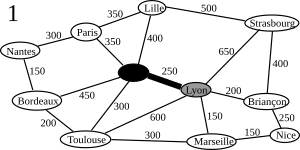
\includegraphics[width=0.5\textwidth]{Prim1.png}}
\framebox{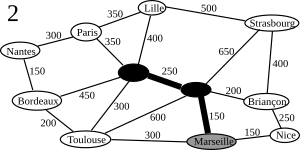
\includegraphics[width=0.5\textwidth]{Prim2.png}}
\framebox{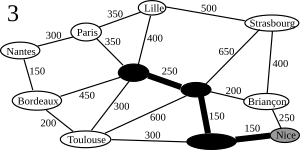
\includegraphics[width=0.5\textwidth]{Prim3.png}}
\framebox{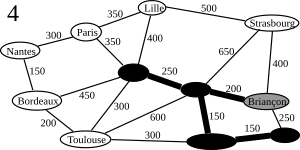
\includegraphics[width=0.5\textwidth]{Prim4.png}}
\framebox{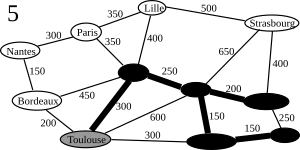
\includegraphics[width=0.5\textwidth]{Prim5.png}}
\framebox{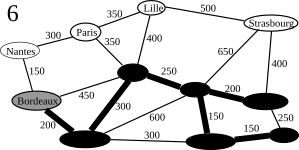
\includegraphics[width=0.5\textwidth]{Prim6.png}}
\framebox{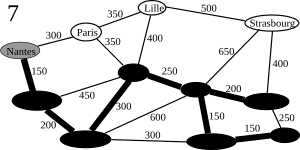
\includegraphics[width=0.5\textwidth]{Prim7.png}}
\framebox{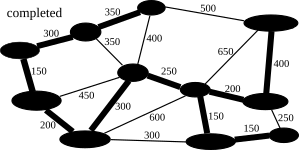
\includegraphics[width=0.5\textwidth]{Prim8.png}}

\caption{The stages of Prim's minimal connecting edge set algorithm. Heavy
lines indicate edges that have been (irrevocably) added to the set.}
\label{prim}
\end{custommargins}
\end{figure}

\afterpage{\clearpage}

And so it goes. In successive frames, we add Marseille, Nice, and Brian\c{c}on
to the set of connected nodes, since we can do no better than 150 km, 150 km,
and 200 km, respectively. Note carefully that in frame 4 we connect
Brian\c{c}on to Lyon -- \textit{not} to Nice -- because $200 <
250$.\footnote{It's very easy to fall into a trance and always add nodes only
to the ends of the growing snake. In fact, I originally did that with this very
example!} Note also that
the algorithm can jump around from side to side --- we aren't looking for the
shortest edge from the most recently added node, but from \textit{any}
connected node.

The final result is shown in the last frame. This is the best way to connect
all the cities to each other, if ``best" means ``least total supply line
distance," which in this case works out to 2450 total kilometers. But if you
look carefully, you'll notice a fascinating thing. \textit{This network of
edges does \textbf{not} contain the shortest path from Bordeaux to Strasbourg!}
I find that result dumbfounding. Wouldn't you think that the shortest path
between any two nodes would land right on this Prim network? Yet if you compare
Figure~\ref{prim} with Figure~\ref{fig:dijkstra} you'll see that the quickest
way from Bordeaux to Strasbourg is through Marseille, not Vichy.

So we end up with the remarkable fact that the shortest route between two
points has nothing whatsoever to do with the shortest \textit{total}
distance between \textit{all} points. Who knew?






\section{Trees}

\index{trees}
A tree is really nothing but a simplification of a graph. There are two
kinds of trees in the world: free trees, and rooted trees.\footnote{There
appears to be no consensus as to which of these concepts is the most basic.
Some authors refer to a free tree simply as a ``tree" --- as though this
were the ``normal" kind of tree --- and use the term rooted tree for the
other kind. Other authors do the opposite. To avoid confusion, I'll try to
always use the full term (although I admit I'm one who considers rooted
trees to be the more important, default concept).}

\subsection{Free trees}

\index{free trees}
A \textbf{free tree} is just a connected graph with no cycles. Every node
is reachable from the others, and there's only one way to get anywhere.
Take a look at Figure~\ref{freetree}. It looks just like a graph (and it
is) but unlike the WWII France graph, it's more skeletal. This is because
in some sense, a free tree doesn't contain anything ``extra."

\begin{figure}[ht]
\centering
\begin{custommargins}{-2.1cm}{-3cm}
  \begin{tikzpicture}
  \node[circle,draw] (C) at (0,0) {C};
  \node[circle,draw] (B) at (-0.3,2) {B};
  \node[circle,draw] (D) at (2,2) {D};
  \node[circle,draw] (E) at (2,-2) {E};
  \node[circle,draw] (A) at (-3,1.7) {A};
  \node[circle,draw] (F) at (-2,-2) {F};
  \draw (F) -- (A) -- (B) -- (C) -- (D);
  \draw (C) -- (E);
  \end{tikzpicture}
\caption{A free tree.}
\label{freetree}
\end{custommargins}
\end{figure}

If you have a free tree, the following interesting facts are true:

\begin{compactenum}
\item There's exactly one path between any two nodes. (Check it!)
\item If you remove any edge, the graph becomes disconnected. (Try it!)
\item If you add any new edge, you end up adding a cycle. (Try it!)
\item \label{onelessedge} If there are $n$ nodes, there are $n-1$ edges. (Think about it!)
\end{compactenum}

So basically, if your goal is connecting all the nodes, and you have a free
tree, you're all set. Adding anything is redundant, and taking away
anything breaks it.

If this reminds you of Prim's algorithm, it should. Prim's algorithm
produced exactly this: a \textit{free tree} connecting all the nodes ---
and specifically the free tree with shortest possible total length. Go back
and look at the final frame of Figure~\ref{prim} and convince yourself that
the darkened edges form a free tree.

\index{Prim's algorithm}
\index{minimal spanning tree}
For this reason, the algorithm is often called \textbf{Prim's minimal
spanning tree algorithm}. A ``spanning tree" just means ``a free tree that
spans (connects) all the graph's nodes." 

Keep in mind that there are many free trees one can make with the same set
of vertices. For instance, if you remove the edge from A to F, and add one
from anything else to F, you have a different free tree.

\subsection{Rooted trees}

\index{trees}
\index{rooted trees}
\index{root (of a tree)}
Now a \textbf{rooted tree} is the same thing as a free tree, except that we
elevate one node to become the \textbf{root}. It turns out this makes all
the difference. Suppose we chose A as the root of Figure~\ref{freetree}.
Then we would have the rooted tree in the left half of
Figure~\ref{rootedtree}. The A vertex has been positioned at the top, and
everything else is flowing under it. I think of it as reaching into the
free tree, carefully grasping a node, and then lifting up your hand so the
rest of the free tree dangles from there. Had we chosen (say) C as the root
instead, we would have a different rooted tree, depicted in the right half
of the figure. Both of these rooted trees have all the same edges as the
free tree did: B is connected to both A and C, F is connected only to A,
\textit{etc.} The only difference is which node is designated the root.

\begin{figure}[ht]
\centering
\begin{custommargins}{-2.1cm}{-3cm}

  \tikz [nodes={circle,draw}]
  \node {A}
  child { node {F} }
  child { node {B}
    child { node {C}
      child { node {D} }
      child { node {E} }
    }
  };
  \quad\quad\quad
  \tikz [nodes={circle,draw}]
  \node {C}
  child { node {B}
    child { node {A}
      child { node {F} } } }
  child { node {D} }
  child { node {E} };

\caption{Two different rooted trees with the same vertices and edges.}
\label{rootedtree}
\end{custommargins}
\label{page:rootedtree}
\end{figure}

\index{spatial positioning}
Up to now we've said that the spatial positioning on graphs is irrelevant.
But this changes a bit with rooted trees. Vertical positioning is our only
way of showing which nodes are ``above" others, and the word ``above" does
indeed have meaning here: it means closer to the root. The altitude of a
node shows how many steps it is away from the root. In the right rooted
tree, nodes B, D, and E are all one step away from the root (C), while node
F is three steps away.

\index{paths (in a graph)}
The key aspect to rooted trees --- which is both their greatest advantage
and greatest limitation --- is that \textit{every node has one and only one
path to the root.} This behavior is inherited from free trees: as we noted,
every node has only one path to every other.

\index{filesystems}
Trees have a myriad of applications. Think of the files and folders on your
hard drive: at the top is the root of the filesystem (perhaps ``\texttt{/}"
on Linux/Mac or ``\texttt{C:}\textbackslash\textbackslash" on Windows) and
underneath that are named folders. Each folder can contain files as well as
other named folders, and so on down the hierarchy. The result is that each
file has one, and only one, distinct path to it from the top of the
filesystem.  The file can be stored, and later retrieved, in exactly one
way.

\index{org charts}
An ``org chart" is like this: the CEO is at the top, then underneath her
are the VP's, the Directors, the Managers, and finally the rank-and-file
employees. So is a military organization: the Commander in Chief directs
generals, who command colonels, who command majors, who command captains,
who command lieutenants, who command sergeants, who command privates.

\index{human body}
The human body is even a rooted tree of sorts: it contains skeletal,
cardiovascular, digestive, and other systems, each of which is comprised of
organs, then tissues, then cells, molecules, and atoms. In fact, anything
that has this sort of part-whole containment hierarchy is just asking to be
represented as a tree.

\index{compilers}
\index{HTML}
\index{chess}
\index{object-oriented design}
In computer programming, the applications are too numerous to name.
Compilers scan code and build a ``parse tree" of its underlying meaning.
HTML is a way of structuring plain text into a tree-like hierarchy of
displayable elements. AI chess programs build trees representing their
possible future moves and their opponent's probable responses, in order to
``see many moves ahead" and evaluate their best options. Object-oriented
designs involve ``inheritance hierarchies" of classes, each one specialized
from a specific other. \textit{Etc.} Other than a simple sequence (like an
array), trees are probably the most common data structure in all of
computer science.

\subsubsection{Rooted tree terminology}

\index{rooted trees}
Rooted trees carry with them a number of terms. I'll use the tree on the
left side of Figure~\ref{rootedtree} as an illustration of each:

\begin{description}
\index{root (of a tree)}
\item[root.] The node at the top of the tree, which is A in our example.
Note that unlike trees in the real world, computer science trees have their
root at the top and grow down. Every tree has a root except the
\textbf{empty tree}, which is the ``tree" that has no nodes at all in it.
(It's kind of weird thinking of ``nothing" as a tree, but it's kind of like
the empty set $\varnothing$, which is still a set.) \index{empty set}

\index{parent (of a node)}
\item[parent.] Every node except the root has one parent: the node
immediately above it. D's parent is C, C's parent is B, F's parent is A,
and A has no parent.

\index{child (of a node)}
\item[child.] Some nodes have children, which are nodes connected directly
below it. A's children are F and B, C's are D and E, B's only child is C,
and E has no children.

\index{sibling (of a node)}
\item[sibling.] A node with the same parent. E's sibling is D, B's is F,
and none of the other nodes have siblings.

\index{ancestor (of a node)}
\item[ancestor.] Your parent, grandparent, great-grandparent,
\textit{etc.}, all the way back to the root. B's only ancestor is A, while
E's ancestors are C, B, and A. Note that F is \textit{not} C's ancestor,
even though it's above it on the diagram: there's no connection from C to
F, except back through the root (which doesn't count).

\index{descendant (of a node)}
\item[descendant.] Your children, grandchildren, great-grandchildren,
\textit{etc.}, all the way to the leaves. B's descendants are C, D and E,
while A's are F, B, C, D, and E. 

\index{leaves}
\item[leaf.] A node with no children. F, D, and E are leaves. Note that in
a (very) small tree, the root could itself be a leaf.

\index{internal nodes}
\item[internal node.] Any node that's not a leaf. A, B, and C are the
internal nodes in our example.

\index{depth (of a node)}
\item[depth (of a node).] A node's depth is the distance (in number of
nodes) from it to the root. The root itself has depth zero. In our example,
B is of depth 1, E is of depth 3, and A is of depth 0.

\index{height (of a tree)}
\item[height (of a tree).] A rooted tree's height is the maximum depth of
any of its nodes; \textit{i.e.}, the maximum distance from the root to any
node. Our example has a height of 3, since the ``deepest" nodes are D and
E, each with a depth of 3. A tree with just one node is considered to have
a height of 0. Bizarrely, but to be consistent, we'll say that the empty
tree has height -1! Strange, but what else could it be? To say it has
height 0 seems inconsistent with a one-node tree also having height 0. At
any rate, this won't come up much.

\index{level (in a tree)}
\item[level.] All the nodes with the same depth are considered on the same
``level." B and F are on level 1, and D and E are on level 3. Nodes on the
same level are \textit{not} necessarily siblings. If F had a child named G
in the example diagram, then G and C would be on the same level (2), but
would \textit{not} be siblings because they have different parents. (We
might call them ``cousins" to continue the family analogy.)

\index{subtree (of a node)}
\index{recursion}
\item[subtree.] \label{recursion} Finally, much of what gives trees their
expressive power is their \textbf{recursive} nature. This means that a tree
is made up of \textit{other (smaller) trees.} Consider our example. It is a
tree with a root of A. But the two children of A are each trees in their
own right! F itself is a tree with only one node. B and its descendants
make another tree with four nodes. We consider these two trees to be
subtrees of the original tree. The notion of ``root" shifts somewhat as we
consider subtrees --- A is the root of the original tree, but B is the root
of the second subtree. When we consider B's children, we see that there is
yet another subtree, which is rooted at C. And so on. It's easy to see that
any subtree fulfills all the properties of trees, and so everything we've
said above applies also to it.

\end{description}

\subsection{Binary trees (BT's)}

\index{binary trees}
\index{left child}
\index{right child}
The nodes in a rooted tree can have any number of children. There's a
special type of rooted tree, though, called a \textbf{binary tree} which we
restrict by simply saying that \textit{each node can have at most two
children.} Furthermore, we'll label each of these two children as the
``left child" and ``right child." (Note that a particular node might well
have \textit{only} a left child, or \textit{only} a right child, but it's
still important to know which direction that child is.)

The left half of Figure~\ref{rootedtree} is a binary tree, but the right
half is not (C has three children). A larger binary tree (of height 4) is
shown in Figure~\ref{binarytree}.

\begin{figure}[ht]
  \centering
    \tikz [grow=down,binary tree layout,nodes={circle,draw}]
    \node {G}
    child { node {K}
      child { node {D}
        child[missing]
        child { node {O}
          child[missing]
          child { node {I} }
        }
      }
      child { node {M}
        child { node {C} }
        child { node {E} }
      }
    }
    child { node {H}
      child { node {A} }
      child { node {B}
        child { node {F} }
        child { node {N}
          child { node {L} }
          child[missing]
        }
      }
    };

\caption{A binary tree.}
\label{binarytree}
\end{figure}

\subsubsection{Traversing binary trees}

\index{traversal}
There were two ways of traversing a graph: breadth-first, and depth-first.
Curiously, there are three ways of traversing a tree: \textbf{pre-order},
\textbf{post-order}, and \textbf{in-order}. All three begin at the root,
and all three consider each of the root's children as subtrees. The
difference is in the order of visitation.

\index{pre-order traversal}

\begin{framed}
To traverse a tree \textbf{pre-order}, we:
\begin{compactenum}
\item Visit the root.
\item Treat the left child and all its descendants as a subtree, and
traverse it in its entirety.
\item Do the same with the right child.
\end{compactenum}
\end{framed}

It's tricky because you have to remember that each time you ``treat a child
as a subtree" you do \textit{the whole traversal process} on that subtree.
This involves remembering where you were once you finish.

Follow this example carefully. For the tree in Figure~\ref{binarytree}, we
begin by visiting G. Then, we traverse the whole ``K subtree." This
involves visiting K itself, and then traversing \textit{its} whole left
subtree (anchored at D). After we visit the D node, we discover that it
actually \textit{has} no left subtree, so we go ahead and traverse its
right subtree. This visits O followed by I (since O has no left subtree
either) which finally returns back up the ladder.

It's at this point where it's easy to get lost. We finish visiting I, and
then we have to ask ``okay, where the heck were we? How did we get here?"
The answer is that we had just been at the K node, where we had traversed
its left (D) subtree. So now what is it time to do? Traverse the
\textit{right} subtree, of course, which is M. This involves visiting M, C,
and E (in that order) before returning to the very top, G. 

Now we're in the same sort of situation where we could have gotten lost
before: we've spent a lot of time in the tangled mess of G's left subtree,
and we just have to remember that it's now time to do G's right subtree.
Follow this same procedure, and the entire order of visitation ends up
being: G, K, D, O, I, M, C, E, H, A, B, F, N, L. (See Figure~\ref{preorder}
for a visual.)

\begin{figure}[ht]
\centering
  \tikz [grow=down,binary tree layout,nodes={circle,draw}, every label/.style={above,draw=none,inner sep=0pt,font=\tiny}]
  \node[label=1] {G}
  child { node[label=2] {K}
    child { node[label=3] {D}
      child[missing]
      child { node[label=4] {O}
        child[missing]
        child { node[label=5] {I} }
      }
    }
    child { node[label=6] {M}
      child { node[label=7] {C} }
      child { node[label=8] {E} }
    }
  }
  child { node[label=9] {H}
    child { node[label=10] {A} }
    child { node[label=11] {B}
      child { node[label=12] {F} }
      child { node[label=13] {N}
        child { node[label=14] {L} }
        child[missing]
      }
    }
  };
\caption{The order of node visitation in \textbf{pre-order} traversal.}
\label{preorder}
\end{figure}

\index{post-order traversal}

\begin{framed}
To traverse a tree \textbf{post-order}, we:
\begin{compactenum}
\item Treat the left child and all its descendants as a subtree, and
traverse it in its entirety.
\item Do the same with the right child.
\item Visit the root.
\end{compactenum}
\end{framed}

It's the same as pre-order, except that we visit the root after the
children instead of before. Still, despite its similarity, this has always
been the trickiest one for me. Everything seems postponed, and you have to
remember what order to do it in later.

For our sample tree, the first node visited turns out to be I. This is
because we have to postpone visiting G until we finish its left (and right)
subtree; then we postpone K until we finish its left (and right) subtree;
postpone D until we're done with O's subtree, and postpone O until we do I.
Then finally, the thing begins to unwind...all the way back up to K. But we
can't actually visit K itself yet, because we have to do its right subtree.
This results in C, E, and M, in that order. \textit{Then} we can do K, but
we still can't do G because we have its whole right subtree's world to
contend with. The entire order ends up being: I, O, D, C, E, M, K, A, F, L,
N, B, H, and finally G. (See Figure~\ref{postorder} for a visual.) 

Note that this is not remotely the reverse of the pre-order visitation, as
you might expect. G is last instead of first, but the rest is all jumbled
up. 

\begin{figure}[ht]
\centering
  \tikz [grow=down,binary tree layout,nodes={circle,draw},every label/.style={above,draw=none,inner sep=0pt,font=\tiny}]
  \node[label=14] {G}
  child { node[label=7] {K}
    child { node[label=3] {D}
      child[missing]
      child { node[label=2] {O}
        child[missing]
        child { node[label=1] {I} }
      }
    }
    child { node[label=6] {M}
      child { node[label=4] {C} }
      child { node[label=5] {E} }
    }
  }
  child { node[label=13] {H}
    child { node[label=8] {A} }
    child { node[label=12] {B}
      child { node[label=9] {F} }
      child { node[label=11] {N}
        child { node[label=10] {L} }
        child[missing]
      }
    }
  };
\caption{The order of node visitation in \textbf{post-order} traversal.}
\label{postorder}
\end{figure}

\index{in-order traversal}

\begin{framed}
Finally, to traverse a tree \textbf{in-order}, we:
\begin{compactenum}
\item \label{inorder:left} Treat the left child and all its descendants as
a subtree, and traverse it in its entirety.
\item Visit the root.
\item Traverse the right subtree in its entirety.
\end{compactenum}
\end{framed}

So instead of visiting the root first (pre-order) or last (post-order) we
treat it in between our left and right children. This might seem to be a
strange thing to do, but there's a method to the madness which will become
clear in the next section.

For the sample tree, the first visited node is D. This is because it's the
first node encountered that doesn't have a left subtree, which means
step~\ref{inorder:left} doesn't need to do anything. This is followed by O
and I, for the same reason. We then visit K before its right subtree, which
in turn visits C, M, and E, in that order. The final order is: D, O, I, K,
C, M, E, G, A, H, F, B, L, N. (See Figure~\ref{inorder}.)

If your nodes are spaced out evenly, you can read the in-order traversal
off the diagram by moving your eyes left to right. Be careful about this,
though, because ultimately the spatial position doesn't matter, but rather
the relationships between nodes. For instance, if I had drawn node I
further to the right, in order to make the lines between D--O--I less
steep, that I node might have been pushed physically to the right of K. But
that wouldn't change the order and have K visited earlier.

\begin{figure}[ht]
\centering
  \tikz [grow=down,binary tree layout,nodes={circle,draw},every label/.style={above,draw=none,inner sep=0pt,font=\tiny}]
  \node[label=8] {G}
  child { node[label=4] {K}
    child { node[label=1] {D}
      child[missing]
      child { node[label=2] {O}
        child[missing]
        child { node[label=3] {I} }
      }
    }
    child { node[label=6] {M}
      child { node[label=5] {C} }
      child { node[label=7] {E} }
    }
  }
  child { node[label=10] {H}
    child { node[label=9] {A} }
    child { node[label=12] {B}
      child { node[label=11] {F} }
      child { node[label=14] {N}
        child { node[label=13] {L} }
        child[missing]
      }
    }
  };
\caption{The order of node visitation in \textbf{in-order} traversal.}
\label{inorder}
\end{figure}

\index{recursion}
Finally, it's worth mentioning that all of these traversal methods make
elegant use of \textbf{recursion}. Recursion is a way of taking a large
problem and breaking it up into similar, but smaller, subproblems. Then,
each of those subproblems can be attacked in the same way as you attacked
the larger problem: by breaking \textit{them} up into subproblems. All you
need is a rule for eventually stopping the ``breaking up" process by
actually doing something.

Every time one of these traversal processes treats a left or right child as
a subtree, they are ``recursing" by re-initiating the whole traversal
process on a smaller tree. Pre-order traversal, for instance, after
visiting the root, says, ``okay, let's pretend we started this whole
traversal thing with the smaller tree rooted at my left child. Once that's
finished, wake me up so I can similarly start it with my right child."
Recursion is a very common and useful way to solve certain complex
problems, and trees are rife with opportunities.

% AI traversal

\subsubsection{Sizes of binary trees}

Binary trees can be any ragged old shape, like our Figure~\ref{binarytree}
example. Sometimes, though, we want to talk about binary trees with a more
regular shape, that satisfy certain conditions. In particular, we'll talk
about three special kinds:

\begin{description}
\index{full binary tree}
\item [full binary tree.] A full binary tree is one in which every node
(except the leaves) has two children. Put another way, every node has
either two children or none: no stringiness allowed.
Figure~\ref{binarytree} is not full, but it would be if we added the three
blank nodes in Figure~\ref{fullbinarytree}.

\begin{figure}[ht]
\centering
  \tikz [grow=down,binary tree layout,nodes={circle,draw}]
  \node {G}
  child { node {K}
    child { node {D}
      child { node {}}
      child { node {O}
        child { node {}}
        child { node {I} }
      }
    }
    child { node {M}
      child { node {C} }
      child { node {E} }
    }
  }
  child { node {H}
    child { node {A} }
    child { node {B}
      child { node {F} }
      child { node {N}
        child { node {L} }
        child { node {} }
      }
    }
  };
\caption{A full binary tree.}
\label{fullbinarytree}
\end{figure}

By the way, it isn't always possible to have a full binary tree with a
particular number of nodes. For instance, a binary tree with two nodes,
can't be full, since it inevitably will have a root with only one child.

\index{complete binary tree}
\item [complete binary tree.] A complete binary tree is one in which every
level has all possible nodes present, except perhaps for the deepest level,
which is filled all the way from the left. Figure~\ref{fullbinarytree} is
not complete, but it would be if we fixed it up as in
Figure~\ref{completebinarytree}.

\begin{figure}[ht]
\centering
  \tikz [grow=down,binary tree layout,nodes={circle,draw}]
  \node {G}
  child { node {K}
    child { node {D}
      child { node {}
        child { node {} }
        child { node {} }
      }
      child { node {O}
        child { node {}}
        child { node {I} }
      }
    }
    child { node {M}
      child { node {C}
        child { node {} }
        child { node {} }
      }
      child { node {E} }
    }
  }
  child { node {H}
    child { node {A}
      child { node {} }
      child { node {L} }
    }
    child { node {B}
      child { node {F} }
      child { node {N} }
    }
  };
\caption{A complete binary tree.}
\label{completebinarytree}
\end{figure}

Unlike full binary trees, it \textit{is} always possible to have a complete
binary tree no matter how many nodes it contains. You just keep filling in
from left to right, level after level.

\index{perfect binary tree}
\item [perfect binary tree.] Our last special type has a rather audacious
title, but a ``perfect" tree is simply one that is exactly balanced: every
level is completely filled. 
Figure~\ref{completebinarytree} is
not perfect, but it would be if we either added nodes to fill out level 4,
or deleted the unfinished part of level 3 (as in
Figure~\ref{perfectbinarytree}.)

\begin{figure}[ht]
\centering
  \tikz [grow=down,binary tree layout,nodes={circle,draw}]
  \node {G}
  child { node {K}
    child { node {D}
      child { node {} }
      child { node {O} }
    }
    child { node {M}
      child { node {C} }
      child { node {E} }
    }
  }
  child { node {H}
    child { node {A}
      child { node {} }
      child { node {I} }
    }
    child { node {B}
      child { node {F} }
      child { node {N} }
    }
  };
\caption{A ``perfect" binary tree.}
\label{perfectbinarytree}
\end{figure}

Perfect binary trees obviously have the strictest size restrictions. It's
only possible, in fact, to have perfect binary trees with $2^{h+1}-1$
nodes, if $h$ is the height of the tree. So there are perfect binary trees
with 1, 3, 7, 15, 31, ... nodes, but none in between. In each such tree,
$2^h$ of the nodes (almost exactly half) are leaves.

\end{description}

\index{heap}
\index{binary search trees}
Now as we'll see, binary trees can possess some pretty amazing powers if
the nodes within them are organized in certain ways. Specifically, a binary
search tree and a heap are two special kinds of binary trees that conform
to specific constraints. In both cases, what makes them so powerful is the
rate at which a tree grows as nodes are added to it.

Suppose we have a perfect binary tree. To make it concrete, let's say it
has height 3, which would give it 1+2+4+8=15 nodes, 8 of which are leaves.
Now what happens if you increase the height of this tree to 4? If it's
still a ``perfect" tree, you will have added 16 more nodes (all leaves).
Thus you have \textit{doubled} the number of leaves by simply adding one
more level. This cascades the more levels you add. A tree of height 5
doubles the number of leaves again (to 32), and height 6 doubles it again
(to 64).

\index{exponential growth}
If this doesn't seem amazing to you, it's probably because you don't fully
appreciate how quickly this kind of \textbf{exponential growth} can
accumulate. Suppose you had a perfect binary tree of height 30 ---
certainly not an awe-inspiring figure. One could imagine it fitting on a
piece of paper...height-wise, that is. But run the numbers and you'll
discover that such a tree would have over \text{half a billion leaves}, more
than one for every person in the United States. Increase the tree's height
to a mere 34 --- just 4 additional levels --- and suddenly you have over 8
billion leaves, easily greater than the population of planet Earth.

The power of exponential growth is only \textit{fully} reached when the
binary tree is perfect, since a tree with some ``missing" internal nodes
does not carry the maximum capacity that it's capable of. It's got some
holes in it. Still, as long as the tree is fairly bushy (\textit{i.e.},
it's not horribly lopsided in just a few areas) the enormous growth
predicted for perfect trees is still approximately the case.

The reason this is called ``exponential" growth is that the quantity we're
varying --- the height --- appears as an \textit{exponent} in the number of
leaves, which is $2^h$. Every time we add just \textit{one} level, we
\textit{double} the number of leaves. 

\index{logarithm}
\index{lg (logarithm base 2)}
So the number of leaves (call it $l$) is $2^h$, if $h$ is the height of the
tree. Flipping this around, we say that $h = \lg(l)$. The function ``lg" is
a logarithm, specifically a logarithm with base-2. This is what computer
scientists often use, rather than a base of 10 (which is written ``log") or
a base of $e$ (which is written ``ln"). Since $2^h$ grows very, very
quickly, it follows that $\lg(l)$ grows very, very slowly. After our tree
reaches a few million nodes, we can add more and more nodes without growing
the height of the tree significantly at all.

The takeaway message here is simply that an incredibly large number of
nodes can be accommodated in a tree with a very modest height. This makes
it possible to, among other things, search a huge amount of information
astonishingly quickly...provided the tree's contents are arranged properly.

\subsection{Binary search trees (BST's)}

\index{binary search trees}
\index{BST property}
Okay, then let's talk about how to arrange those contents. A \textbf{binary
search tree} (BST) is any binary tree that satisfies one additional
property: \textit{every node is ``greater than" all of the nodes in its
left subtree, and ``less than (or equal to)" all of the nodes in its right
subtree.} We'll call this \textbf{the BST property}. The phrases ``greater
than" and ``less than" are in quotes here because their meaning is somewhat
flexible, depending on what we're storing in the tree.  If we're storing
numbers, we'll use numerical order. If we're storing names, we'll use
alphabetical order. Whatever it is we're storing, we simply need a way to
compare two nodes to determine which one ``goes before" the other.

An example of a BST containing people is given in Figure~\ref{bst}. Imagine
that each of these nodes contains a good deal of information about a
particular person --- an employee record, medical history, account
information, what have you. The nodes themselves are indexed by the
person's name, and the nodes are organized according to the BST rule. Mitch
comes after Ben/Jessica/Jim and before Randi/Owen/Molly/Xander in
alphabetical order, and this ordering relationship between parents and
children repeats itself all the way down the tree. (Check it!)

\begin{figure}[ht]
\centering
  \tikz [grow=down,binary tree layout,nodes={circle,draw}]
  \node {Mitch} {
    child { node {Jessica}
      child { node {Ben} }
      child { node {Jim} }
    }
    child { node {Randi}
      child { node {Owen}
        child { node {Molly} }
        child[missing]
      }
      child { node {Xander} }
    }
  };
\caption{A binary search tree.}
\label{bst}
\end{figure}

Be careful to observe that the ordering rule applies between a node and the
\textit{entire} contents of its subtrees, not merely to its immediate
children. This is a rookie mistake that you want to avoid. Your first
inclincation, when glancing at Figure~\ref{falsebst}, below, is to judge it
a BST. It is \textit{not} a binary search tree, however! Jessica is to the
left of Mitch, as she should be, and Nancy is to the right of Jessica, as
she should be. It seems to check out. But the problem is that Nancy is a
descendant of Mitch's \textit{left} subtree, whereas she must properly be
placed somewhere in his \textit{right} subtree. And yes, this matters. So
be sure to check your BST's all the way up and down.

\begin{figure}[ht]
\centering
  \tikz [grow=down,binary tree layout,nodes={circle,draw}]
  \node[fill=gray] {Mitch} {
    child { node {Jessica}
      child { node {Ben} }
      child { node[fill=gray] {Nancy} }
    }
    child { node {Randi}
      child { node {Owen}
        child { node {Molly} }
        child[missing]
      }
      child { node {Xander} }
    }
  };
\caption{\textbf{NOT} a binary search tree, though
it looks like one at first glance. (Notice Nancy and Mitch)}
\label{falsebst}
\end{figure}

\subsubsection{The power of BST's}

All right, so what's all the buzz about BST's, anyway? The key insight is
to realize that if you're looking for a node, all you have to do is start
at the root and go \textit{the height of the tree down} making one
comparison at each level. Let's say we're searching Figure~\ref{bst} for
Molly. By looking at Mitch (the root), we know right away that Molly must
be in the right subtree, not the left, because she comes \textit{after}
Mitch in alphabetical order. So we look at Randi. This time, we find that
Molly comes \textit{before} Randi, so she must be somewhere in Randi's left
branch. Owen sends us left again, at which point we find Molly.

\index{New York City}
With a tree this size, it doesn't seem that amazing. But suppose its height
were 10. This would mean about 2000 nodes in the tree --- customers, users,
friends, whatever. With a BST, you'd only have to examine \textit{ten} of
those 2000 nodes to find whatever you're looking for, whereas if the nodes
were just in an ordinary list, you'd have to compare against 1000 or so of
them before you stumbled on the one you were looking for. And as the size
of the tree grows, this discrepancy grows (much) larger. If you wanted to
find a single person's records in New York City, would you rather search 7
million names, or 24 names?? Because that's the difference you're looking
at.

It seems almost too good to be true. How is such a speedup possible? The
trick is to realize that with every node you look at, you effectively
eliminate \textit{half of the remaining tree} from consideration. For
instance, if we're looking for Molly, we can disregard Mitch's entire left
half without even looking at it, then the same for Randi's entire right
half. If you discard half of something, then half of the remaining half,
then half again, it doesn't take you long before you've eliminated almost
every false lead.

\index{Big-O notation}
\index{O(n) algorithm}
\index{algorithm}
There's a formal way to describe this speedup, called ``Big-O notation."
The subtleties are a bit complex, but the basic idea is this. When we say
that an algorithm is ``O(n)" (pronounced ``oh--of--n"), it means that the
time it takes to execute the algorithm is \textit{proportional to the
number of nodes.} This doesn't imply any specific number of milliseconds or
anything --- that is highly dependent on the type of computer hardware, you
have, the programming language, and a myriad of other things. But what we
\textit{can} say about an O(n) algorithm is that if you double the number
of nodes, you're going to approximately double the running time. If you
quadruple the number of nodes, you're going to quadruple the running time.
This is what you'd expect.

Searching for ``Molly" in a simple unsorted list of names is an O(n)
prospect. If there's a thousand nodes in the list, on average you'll find
Molly after scanning through 500 of them. (You might get lucky and find
Molly at the beginning, but then of course you might get really unlucky and
not find her until the end. This averages out to about half the size of the
list in the normal case.) If there's a \textit{million} nodes, however,
it'll take you 500,000 traversals on average before finding Molly. Ten
times as many nodes means ten times as long to find Molly, and a thousand
times as many means a thousand times as long. Bummer.

\index{O(lg n) algorithm}
\index{algorithm}
Looking up Molly in a BST, however, is an O(lg n) process. Recall that
``lg" means the logarithm (base-2). This means that doubling the number of
nodes gives you a \textit{miniscule} increase in the running time. Suppose
there were a thousand nodes in your tree, as above. You wouldn't have to
look through 500 to find Molly: you'd only have to look through
\textit{ten} (because $\lg(1000) \approx 10$). Now increase it to a million
nodes. You wouldn't have to look through 500,000 to find Molly: you'd only
have to look through \textit{twenty}. Suppose you had 6 billion nodes in
your tree (approximately the population of the earth). You wouldn't have to
look through 3 billion nodes: you'd only have to look through
\textit{thirty-three}. Absolutely mind-boggling.

\subsubsection{Adding nodes to a BST}

Finding things in a BST is lightning fast. Turns out, so is adding things
to it. Suppose we acquire a new customer named Jennifer, and we need to add
her to our BST so we can retrieve her account information in the future.
All we do is follow the same process we would if we were \textit{looking}
for Jennifer, but as soon as we find the spot where she would be, we add
her there. In this case, Jennifer comes before Mitch (go left), and before
Jessica (go left again), and after Ben (go right). Ben has no right child,
so we put Jessica in the tree right at that point. (See
Figure~\ref{bstadd1}.)

\begin{figure}[ht]
\centering
\begin{custommargins}{-2.1cm}{-3cm}

  \tikz [grow=down,binary tree layout,nodes={circle,draw}]
  \node {Mitch} {
    child { node {Jessica}
      child { node {Ben} }
      child { node {Jim} }
    }
    child { node {Randi}
      child { node {Owen}
        child { node {Molly} }
        child[missing]
      }
      child { node {Xander} }
    }
  };
  \quad
  \tikz [grow=down,binary tree layout,nodes={circle,draw}]
  \node {Mitch} {
    child { node {Jessica}
      child { node {Ben}
        child[missing]
        child { node[fill=gray] {Jennifer} }
      }
      child { node {Jim} }
    }
    child { node {Randi}
      child { node {Owen}
        child { node {Molly} }
        child[missing]
      }
      child { node {Xander} }
    }
  };
\caption{The BST after adding Jennifer.}
\label{bstadd1}
\end{custommargins}
\end{figure}

\index{O(lg n) algorithm}
\index{algorithm}
This adding process is also an O(lg n) algorithm, since we only need look
at a small number of nodes equal to the height of the tree.

\index{leaves}
Note that a new entry always becomes a \textit{leaf} when added. In fact,
this allows us to look at the tree and reconstruct some of what came
before. For instance, we know that Mitch must have been the first node
originally inserted, and that Randi was inserted before Owen, Xander, or
Molly. As an exercise, add your own name to this tree (and a few of your
friends' names) to make sure you get the hang of it. When you're done the
tree must of course obey the BST property.

\subsubsection{Removing nodes from a BST}

Removing nodes is a bit trickier than adding them. How do we delete an
entry without messing up the structure of the tree? It's easy to see how to
delete Molly: since she's just a leaf, just remove her and be done with it.
But how to delete Jessica? Or for that matter, Mitch?

Your first inclination might be to eliminate the node and promote one of its
children to go up in its place. For instance, if we delete Jessica, you might
think we could just elevate Ben up to where Jessica was, and then move Jennifer
up under Ben as well. This doesn't work, though. The result would look like
Figure~\ref{bstremovewrong}, with Jennifer in the wrong place. The next time we
look for Jennifer in the tree, we'll search to the \textit{right} of Ben (as we
should), completely missing her. Jennifer has effectively been lost.

\begin{figure}[ht]
\centering
  \begin{custommargins}{-2.1cm}{-3cm}
  \tikz [grow=down,binary tree layout,nodes={circle,draw}]
  \node {Mitch} {
    child { node[dashed] {Jessica}
      child { node {Ben}
        child[missing]
        child { node {Jennifer} }
      }
      child { node {Jim} }
    }
    child { node {Randi}
      child { node {Owen}
        child { node {Molly} }
        child[missing]
      }
      child { node {Xander} }
    }
  };
  \quad
  \tikz [grow=down,binary tree layout,nodes={circle,draw}]
  \node {Mitch} {
    child { node[fill=gray] {Ben}
      child { node[fill=gray] {Jennifer}
        edge from parent
        node[above,sloped,loosely dotted] {!}
      }
      child { node {Jim} }
    }
    child { node {Randi}
      child { node {Owen}
        child { node {Molly} }
        child[missing]
      }
      child { node {Xander} }
    }
  };
\caption{A \textbf{wrong} (non)-BST after removing Jessica incorrectly.}
\label{bstremovewrong}
\end{custommargins}
\end{figure}

One correct way (there are others) to do a node removal is to replace the node
with \textit{the left-most descendant of its right subtree}. (Or, equivalently,
the right-most descendant of its left subtree). Let's be careful to define
this: to get the left-most descendant of a node's right subtree, we (1) go to
the \textit{right} child of the node, and then (2) go
as-left-as-we-possibly-can from there, until we come to a node that has no
left child. That node (the one without a left child) is officially the
left-most descendent of the original node's right subtree.

Example: flip back to Figure~\ref{binarytree} (p.~\pageref{binarytree}). What
is the left-most descendent of G's right subtree? Answer: A. We start by going
right from G down to H, and then we go as-left-as-possible...which turns out to
be only one node's worth of ``left,'' because we hit A, and A has no left child
(or right child, for that matter.) Work these additional examples out for
yourself: what is the left-most descendent of K's right subtree? Of D's? Of
H's?\footnote{Answers: The left-most descendent of K's right subtree is
\textbf{C}, of D's right subtree is \textbf{O}, and of H's, \textbf{F}.}

Okay, let's return to Figure~\ref{bstadd1} (p.~\pageref{bstadd1}) and remove
Jessica the \textit{correct} way. We simply find the left-most descendent of
her right subtree -- namely, Jim -- and promote him in place of her.
Figure~\ref{bstremoveright} shows the result. Note that we replaced her with
Jim \textit{not} because it's okay to blindly promote her right child, but
because \textit{Jim had no left descendants}, and hence he was the left-most
node in her right subtree. (If he \textit{had} left descendents, promoting him
would have been just as wrong as promoting Ben. Instead, we would have gone
left from Jim until we couldn't go left anymore, and promoted \textit{that}
node.)

\begin{figure}[ht]
\centering
\begin{custommargins}{-2.1cm}{-3cm}

  \tikz [grow=down,binary tree layout,nodes={circle,draw}]
  \node {Mitch} {
    child { node[dashed] {Jessica}
      child { node {Ben}
        child[missing]
        child { node {Jennifer} }
      }
      child { node {Jim} }
    }
    child { node {Randi}
      child { node {Owen}
        child { node {Molly} }
        child[missing]
      }
      child { node {Xander} }
    }
  };
  \quad
  \tikz [grow=down,binary tree layout,nodes={circle,draw}]
  \node {Mitch} {
    child { node[fill=gray] {Jim}
      child { node {Ben}
        child[missing]
        child { node {Jennifer} }
      }
      child[missing]
    }
    child { node {Randi}
      child { node {Owen}
        child { node {Molly} }
        child[missing]
      }
      child { node {Xander} }
    }
  };
\caption{The BST after removing Jessica correctly.}
\label{bstremoveright}
\end{custommargins}
\end{figure}

As another example, let's go whole-hog and remove the root node, Mitch. The
result is as shown in Figure~\ref{bstremoveright2}. It's rags-to-riches for
Molly: she got promoted from a leaf all the way to the top. Why Molly?
Because she was the left-most descendant of Mitch's right subtree.

\begin{figure}[ht]
\centering
  \begin{custommargins}{-2.1cm}{-3cm}
  \tikz [grow=down,binary tree layout,nodes={circle,draw}]
  \node[dashed] {Mitch} {
    child { node {Jim}
      child { node {Ben}
        child[missing]
        child { node {Jennifer} }
      }
      child[missing]
    }
    child { node {Randi}
      child { node {Owen}
        child { node {Molly} }
        child[missing]
      }
      child { node {Xander} }
    }
  };
  \quad
  \tikz [grow=down,binary tree layout,nodes={circle,draw}]
  \node[fill=gray] {Molly} {
    child { node {Jim}
      child { node {Ben}
        child[missing]
        child { node {Jennifer} }
      }
      child[missing]
    }
    child { node {Randi}
      child { node {Owen} }
      child { node {Xander} }
    }
  };
\caption{The BST after removing Mitch.}
\label{bstremoveright2}
\end{custommargins}
\end{figure}

\index{in-order traversal}
\index{BST property}
To see why this works, just consider that \textit{Molly was immediately
after Mitch in alphabetical order.} The fact that he was a king and she a
peasant was misleading. The two of them were actually very close:
consecutive, in fact, with in-order traversal. So replacing Mitch with
Molly avoids shuffling anybody out of alphabetical order, and preserves the
all-important BST property.

\subsection{Balancedness}
\index{balancedness (of a tree)}

\index{O(n) algorithm}
\index{algorithm}
Finally, recall that this amazingly fast lookup is critically dependent on
the tree being ``bushy." Otherwise, the approximation that $h=\lg(l)$
breaks down. As a laughably extreme example, consider
Figure~\ref{bstunbalanced}, which contains the same nodes we've been using.
This is a legitimate binary search tree! (Check it!) Yet looking up a node
in this monstrosity is obviously not going to be any faster than looking it
up in a plain-old list. We're back to O(n) performance.

\begin{figure}[ht]
\centering
  \tikz [grow=down,binary tree layout,nodes={circle,draw}]
  \node {Ben} {
    child[missing]
    child { node {Jennifer} {
        child[missing]
        child { node {Jim} {
            child[missing]
            child { node {Molly} {
                child[missing]
                child { node {Owen} {
                    child[missing]
                    child { node {Randi} {
                        child[missing]
                        child { node {Xander} }
                      }
                    }
                  }
                }
              }
            }
          }
        }
      }
    }
  };
\caption{An incredibly bad, but still technically legit, BST.}
\label{bstunbalanced}
\end{figure}

In practice, there are three ways of dealing with this. One approach is to
simply not worry about it. After all, as long as we're inserting and
removing nodes randomly, with no discernable pattern, the chances of
obtaining a tree as lopsided as Figure~\ref{bstunbalanced} are
astronomically small. It's as likely as throwing a deck of cards up in the
air and having it land all in a neat stack. The law of entropy tells us
that we're going to get a mix of short branches and long branches, and that
in a large tree, the unbalancedness will be minimal.

\index{rebalancing (a tree)}
A second approach is to periodically rebalance the tree. If our website
goes offline for maintenance every once in a while anyway, we could rebuild
our tree from the ground up by inserting the nodes into a fresh tree in a
beneficial order. What order should we insert them in? Well, remember that
whichever node is inserted first will be the root. This suggests that we'd
want to insert the \textit{middle} node first into our tree, so that Molly
becomes the new root. This leaves half the nodes for her left subtree and
half for her right. If you follow this process logically (and recursively)
you'll realize that we'd next want to insert the middle nodes \textit{of
each half.} This would equate to Jennifer and Randi (in either order). I
think of it like the markings on a ruler: first you insert half an inch,
then $\frac{1}{4}$ and $\frac{3}{4}$ inches, then $\frac{1}{8}$,
$\frac{3}{8}$, $\frac{5}{8}$, and $\frac{7}{8}$ inches, \textit{etc.} This
restores to us a perfectly balanced tree at regular intervals, making any
large imbalances even more improbable (and short-lived).

\index{AVL trees}
\index{red-black trees}
Thirdly, there are specialized data structures you may learn about in
future courses, such as AVL trees and red-black trees, which are binary
search trees that add extra rules to prevent imbalancing. Basically, the
idea is that when a node is inserted (or removed), certain metrics are
checked to make sure that the change didn't cause too great an imbalance.
If it did, the tree is adjusted so as to minimize the imbalance. This comes
at a slight cost every time the tree is changed, but prevents any
possibility of a lopsided tree that would cause slow lookups in the long
run.

\section{Final word}

Whew, that was a lot of information about structures. Before we continue
our walk in the next chapter with a completely different topic, I'll leave
you with this summary thought. Let $BST$ be the set of Binary Search Trees,
and $BT$ be the set of Binary Trees. Let $RT$ be the set of rooted trees,
and $T$ be the set of trees (free or rooted). Finally, let $CG$ be the set
of connected graphs, and $G$ the set of all graphs. Then we have:

\[
BST \subset BT \subset RT \subset T \subset CG \subset G.
\]

It's a beautiful thing.


\section{Exercises}

\begin{small}
\begin{enumerate}
\newcolumntype{Q}{>{\arraybackslash}m{.45\textwidth}}
\newcolumntype{A}{>{\arraybackslash}m{.5\textwidth}}
%\begin{longtable}{m{0.3\textwidth} || m{0.6\textwidth}}
\begin{longtable}{Q || A}
\hline
\vspace{-.2in}
\item How many vertices are there in the graph below?
\begin{center}
  \resizebox{0.4\textwidth}{!}{
    \begin{tikzpicture}
      \graph [grow=down,layered layout,nodes={circle,draw,fill=lightgray},edges={bend left}] {
        D --[bend right] C;
        A --[bend right] F;
        A -- { E, B };
        F -- E -- B -- F;
      };
    \end{tikzpicture}
  }
\end{center}
&
6.\\
\hline
\item How many edges are there?
&
7.\\
\hline
\item What's the degree of vertex \textsl{B}?
&
3.\\
\hline
\item Is this graph directed?
&
No. (No arrowheads on the lines.)\\
\hline
\item Is this graph connected?
&
No -- there is no path from \textsl{A}, \textsl{B}, \textsl{E}, or \textsl{F}
to either \textsl{C} or \textsl{D}.\\
\hline
\item Is this graph weighted?
&
No. (No numbers annotating the edges.)\\
\hline
\item Is it a tree?
&
No. (A tree must be connected, and must also have no cycles, which this graph
clearly does: \textit{e.g.},
\textsl{B}--to--\textsl{A}--to--\textsl{E}--to--\textsl{B}.)\\
\hline
\item Is it a DAG?
&
Not remotely: it is neither directed nor acyclic.\\
\hline
\item If this graph represented an endorelation, how many ordered pairs would
it have?
&
14. (If you said 7, remember that since there are no arrowheads on the lines,
this is an undirected graph, which corresponds to a symmetric relation, and
hence both (\textsl{A}, \textsl{E}) and (\textsl{E}, \textsl{A}) will be
present.)\\


\hline
\vspace{-.2in}
\item How many vertices and edges are there in the graph below?
\begin{center}
  \resizebox{0.4\textwidth}{!}{
    \begin{tikzpicture}
      \graph [grow'=down,layered layout,nodes={draw,circle,fill=lightgray},node sep=4em,sibling distance=4em,edges={-latex,bend right}] {
        M --[bend left] K --[bend left] J;
        H -- {G -- L -- I -- J, L, I};
        I -- G --[bend left] M;
      };
    \end{tikzpicture}
  }
\end{center}
&
7 and 10, respectively.\\
\hline
\vspace{-.2in}
\item What's the degree of vertex \textsl{L}?
&
\footnotesize
It has an in-degree of 2, and an out-degree of 1.\\
\hline
\normalsize
\vspace{-.2in}
\item Is this graph directed?
&
\footnotesize
Yes.\\
\hline
\normalsize
\item Is this graph connected?
&
\scriptsize
Depends on what we mean. There are two different notions of ``connectedness''
for directed graphs. One is \textbf{strongly connected}, which means every
vertex is reachable from any other by following the arrows in their specified
directions. By that definition, this graph is not connected: there's no way to
get to \textsl{H} from \textsl{J}, for example. It is \textbf{weakly
connected}, however, which means that if you \textit{ignore} the arrowheads and
consider it like an unidirected graph, it would be connected.\\
\hline
\normalsize
\item Is it a tree?
&
\scriptsize
No. For one thing, a tree can't have any ``extra'' edges beyond what's
necessary to make it connected, and there's redundancy galore here.\\
\hline
\normalsize
\item Is it a DAG?
&
\scriptsize
Allllmost. If you look very carefully, you'll see that there is indeed a cycle:
\textsl{I}--to--\textsl{G}--to--\textsl{L}. So if this graph were to represent
a recipe or project workflow, it would be impossible to complete.\\
\hline
\normalsize
\vspace{-.2in}
\item If we reversed the direction of the \textsl{I}--to--\textsl{G} edge,
would it be a DAG?
&
\footnotesize
Yes. The steps could now be completed in this order: \textsl{H}, \textsl{G},
\textsl{L}, \textsl{I}, \textsl{M}, \textsl{K}, and finally \textsl{J}.\\
\hline
\normalsize
\vspace{-.2in}
\item If this graph represented an endorelation, how many ordered pairs would
it have?
&
\footnotesize
10.\\
\hline
\vspace{-.2in}
\item Suppose we traversed the graph below in depth-first fashion, starting
with node \textsl{P}. In what order would we visit the nodes?
\begin{center}
  \resizebox{0.4\textwidth}{!}{
    \begin{tikzpicture}
      \graph [grow'=down,simple necklace layout,nodes={draw,circle,fill=lightgray},node sep=3em,edges={bend left}] {
        N -- O -- P -- Q -- R -- S -- T -- N;
      };
    \end{tikzpicture}
  }
\end{center}
&
There are two possible answers: \textsl{P}, \textsl{Q}, \textsl{R}, \textsl{S}, \textsl{T}, \textsl{N}, \textsl{O}, or else \textsl{P}, \textsl{O}, \textsl{N}, \textsl{T}, \textsl{S}, \textsl{R},
\textsl{Q}. (The choice just depends on whether we go ``left'' or ``right''
initially.) Note in particular that either \textsl{O} or \textsl{Q} is at the very end of the
list.\\
\hline
\vspace{-.2in}
\item Now we traverse the same graph breadth-first fashion, starting
with node \textsl{P}. Now in what order would we visit the nodes?
&
Again, two possible answers: \textsl{P}, \textsl{O}, \textsl{Q}, \textsl{N}, \textsl{R}, \textsl{T}, \textsl{S}, or else \textsl{P}, \textsl{Q}, \textsl{O}, \textsl{R}, \textsl{N}, \textsl{S},
\textsl{T}. Note in particular that both \textsl{O} and \textsl{Q} are visited
very early.\\
\hline
\item If we traversed the tree below in pre-order fashion, in what order would
we visit the nodes?
\begin{center}
  \resizebox{0.4\textwidth}{!}{
    \begin{tikzpicture}
      \graph [grow=down,binary tree layout,nodes={draw,circle,fill=lightgray}] {
        G -- { S -- {Y -- {H, E}, }, W -- {D -- {, P -- {, U}}, A }};
      };
    \end{tikzpicture}
  }
\end{center}
&
\textsl{G}, \textsl{S}, \textsl{Y}, \textsl{H}, \textsl{E}, \textsl{W},
\textsl{D}, \textsl{P}, \textsl{U}, \textsl{A}.\\
\hline
\vspace{-.2in}
\item What if we traversed it in in-order fashion?
&
\textsl{H}, \textsl{Y}, \textsl{E}, \textsl{S}, \textsl{G}, \textsl{D},
\textsl{P}, \textsl{U}, \textsl{W}, \textsl{A}.\\
\hline
\vspace{-.2in}
\item What if we traversed it in post-order fashion?
&
\textsl{H}, \textsl{E}, \textsl{Y},\ \ \textsl{S}, \textsl{U}, \textsl{P},
\ \textsl{D}, \textsl{A}, \textsl{W}, \textsl{G}.\\
\hline
\item Is the graph below a tree?
\begin{center}
  \resizebox{0.4\textwidth}{!}{
    \begin{tikzpicture}
      \graph [grow=down,binary tree layout,nodes={draw,circle,fill=lightgray},sibling distance=5em,level distance=1em] {
        Mal -- { Jayne -- {Inara, Kaylee}, Wash -- {River -- {, Simon -- {, Zoe}}, }};
      };
    \end{tikzpicture}
  }
\end{center}
&
Yes. (Every node has one and only one path to the root, and to every other node
for that matter.)\\
\hline
\item Is it a binary tree?
&
Yes. (Every node has at most two children, and they are clearly pictured as
being a ``left'' child and/or a ``right'' child.)\\
\hline
\item Is it a binary search tree?
&
No. Although nearly every node does satisfy the BST property (all the nodes in
its left subtree come before it alphabetically, and all the nodes in its right
subtree come after it), there is a single exception: \textsl{Zoe} is in
\textsl{Wash}'s left subtree, whereas she should be to his right.\\
\hline
\item How could we fix it?
&
Many ways; one would be to swap \textsl{Zoe}'s and \textsl{Wash}'s positions.
If we do that, the fixed tree would be:
\begin{center}
  \resizebox{0.4\textwidth}{!}{
    \begin{tikzpicture}
      \graph [grow=down,binary tree layout,nodes={draw,circle,fill=lightgray}] {
        Mal -- { Jayne -- {Inara, Kaylee}, Zoe -- {River -- {, Simon -- {, Wash}}, }};
      };
    \end{tikzpicture}
  }
\end{center} Take a moment and convince yourself that every node of this new
tree does in fact satisfy the BST property.\\
\hline
\item Is the tree balanced?
&
It's not too bad, but it does have one too many levels in it (it has a height
of 4, whereas all its nodes would fit in a tree of height 3).\\
\hline
\item How could we make it more balanced?
&
Many ways; one would be to rotate the
\textsl{River}--\textsl{Simon}--\textsl{Wash} threesome so that \textsl{Simon}
becomes \textsl{Zoe}'s left child. \textsl{Simon} would then be the parent of
\textsl{River} (on his left) and \textsl{Wash} (on his right).\\
\hline
\item If we wanted to add a new node called ``\textsl{Shepherd}'' to this tree,
where would he go?
&
To \textsl{Simon}'s left.\\
\hline
\item If we wanted to remove the ``\textsl{Mal}'' node from this tree, how
would we do that?
&
We can put the left-most node of \textsl{Mal}'s right subtree (that would be
\textsl{River}) in \textsl{Mal}'s place, and then make \textsl{Simon} (and
everything under him) become \textsl{Wash}'s left child. The result would look
like this:
\begin{center}
  \resizebox{0.4\textwidth}{!}{
    \begin{tikzpicture}
      \graph [grow=down,binary tree layout,nodes={draw,circle,fill=lightgray}] {
        River -- { Jayne -- {Inara, Kaylee}, Zoe -- {Simon -- {, Wash}, }};
      };
    \end{tikzpicture}
  }
\end{center}
Take a moment and convince yourself that this \textsl{Mal}-less
tree does in fact satisfy the BST property.\\
\hline
\end{longtable}
\end{enumerate}
\end{small}


\chapter{Counting}

If the title of this chapter seems less than inspiring, it's only because
the kind of counting we learned as children was mostly of a straightforward
kind. In this chapter, we're going to learn to answer some more difficult
questions like ``how many different semester schedules could a college
student possibly have?" and ``how many different passwords can a
customer choose for this e-commerce website?" and ``how likely is this
network buffer to overflow, given that its packets are addressed to three
different destinations?"

\index{combinatorics}
\index{enumerating}
\smallskip
The more impressive-sounding name for this topic is \textbf{combinatorics}.
In combinatorics, we focus on two tasks: counting things (to find out how
many there are), and enumerating things (to systematically list them as
individuals). Some things turn out to be hard to count but easy to
enumerate, and vice versa.
\bigskip
\bigskip
\bigskip

\pagebreak
\section{The Fundamental Theorem}

\index{Fundamental Theorem of Counting}
We start with a basic rule that goes by the audacious name of \textbf{The
Fundamental Theorem of Counting}.\footnote{How many other ``Fundamental
Theorems" of math do you know? Here are a few: the Fundamental Theorem of
Arithmetic says that any natural number can be broken down into its prime
factors in only one way. The Fundamental Theorem of Algebra says that the
highest power of a polynomial is how many roots (zeroes) it has. The
Fundamental Theorem of \textit{Linear} Algebra says that the row space and the
column space of a matrix have the same dimension. The Fundamental Theorem of
Calculus says that integration and differentiation are the inverse of each
other.} It goes like this:

\begin{framed}
If a whole can be divided into $k$ parts, and
there's $n_i$ choices for the $i^{\text{th}}$ part, then there's $n_1
\times n_2 \times n_3 \times \cdots \times n_k$ ways of doing the whole
thing.
\end{framed}


Example: Jane is ordering a new Lamborghini. She has twelve different
paint colors to choose from (including Luscious Red and Sassy Yellow),
three different interiors (Premium Leather, Bonded Leather, or Vinyl), and
three different stereo systems. She must also choose between automatic and
manual transmission, and she can get power locks \& windows (or not). How
many different configurations does Jane have to choose from? Put another
way, how many different kinds of cars could come off the line for her?

The key is that every one of her choices is independent of all the others.
Choosing an Envious Green exterior doesn't constrain her choice of
transmission, stereo, or anything else. So no matter which of the 12 paint
colors she chooses, she can independently choose any of the three
interiors, and no matter what these first two choices were, she can freely
choose any of the stereos, \textit{etc.} It's a mix-and-match. Therefore
the answer is:

\[
12 \times 3 \times 3 \times 2 \times 2 = 432\ \text{choices}.
\]

Here's an alternate notation you'll run into for this, by the way:

\index{product operator ($\Pi$)}
\[
\prod_{i=1}^k{n_i}
\]
which is just a shorter way of writing
\[
n_1 \times n_2 \times n_3 \times \cdots \times n_k.
\]

\index{summation operator ($\Sigma$)}
As mentioned in section~\ref{totalprob}, the $\Sigma$ notation is
essentially a loop with a counter, and it says to add up the expression to
the right of it for each value of the counter. The $\Pi$ notation is
exactly the same, only instead of adding the expressions together for each
value of the counter, we're multiplying them. (The reason mathematicians
chose the symbols $\Sigma$ (sigma) and $\Pi$ (pi) for this, by the way, is
that ``sigma" and ``pi" start with the same letter as ``sum" and
``product," respectively.)

\index{ATM machines}
\index{PINs}
We can actually get a lot of leverage just with the fundamental theorem.
How many different PINs are possible for an ATM card? There are four
digits, each of which can be any value from 0 to 9 (ten total values), so
the answer is:

\[
10 \times 10 \times 10 \times 10 = 10,000\ \text{different PINs}.
\]

So a thief at an ATM machine frantically entering PINs at random (hoping to
break your account before you call and stop your debit card) would have to
try about 5,000 of them on average before cracking the code.

\index{locker combinations}
What about middle school bullies who are trying to break into your locker?
Well, most combination locks are opened by a three-number sequence, each
number of which is anything from 0 to 39. So there are:

\[
40 \times 40 \times 40 = 64,000\ \text{different combinations}.
\]

That's probably slightly overstated, since I'll bet consecutive repeat
numbers are not allowed (Master probably doesn't manufacture a lock with a
combination of 17--17--23, for example.) But it does seem at least as
secure as a PIN number.

\index{license plates}
\label{license plates}
Every car in the state of Virginia must be issued its own license plate
number. That's a lot of cars. How many different license plate combinations
are available?

This one requires a bit more thought, since not all licenses numbers have
the same number of characters. In addition to ``\texttt{SED4756}" and
``\texttt{PXY1927}" you can also have ``\texttt{DAWG}" or ``\texttt{LUVME}"
or even ``\texttt{U2}". How can we incorporate these?

\index{mutually exclusive}
The trick is to divide up our set into mutually exclusive subsets, and then
add up the cardinalities of the subsets. If only 7 characters fit on a
license plate, then clearly every license plate number has either 1, 2, 3,
4, 5, 6, or 7 characters. And no license plate has \textit{two} of these
(\textit{i.e.}, there is no plate that is both 5 characters long
\textit{and} 6 characters long). Therefore they're mutually exclusive
subsets, and safe to add. This last point is often not fully appreciated,
leading to errors. Be careful not to cavalierly add the cardinalities of
non-mutually-exclusive sets! You'll end up double-counting items.

So we know that the number of possible license plates is equal to:
\begin{center}
the \# of 7-character plates + \\
the \# of 6-character plates + \\
the \# of 5-character plates + \\
$\cdots$ + \\
the \# of 1-character plates.
\end{center}

Very well. We can now figure out each one separately. How do we know how
many 7-character plates there are? Well, if every character must be either
a letter or a digit, then we have 26 + 10 = 36 choices for each character.
This implies $36^7$ different possible 7-character license plates. The
total number of plates is therefore:
\[
36^7 + 36^6 + 36^5 + 36^4 + 36^3 + 36^2 + 36 = \text{80,603,140,212 plates}
\]

which is about ten times the population of the earth, so I think we're
safe for now.

Here's an interesting thought experiment to test your intuition about
numbers. Look at the above calculation, and ask yourself: ``what if the
state of Virginia decided, for purposes of consistency, that all license
plates \textit{had} to have the full 7 characters? Would that significantly
reduce the total number of possible plates?" My first inclination would be
to say ``yes," because we're adding seven things in that equation, and if
we mandated 7-character plates for everyone we'd eliminate 6 out of the 7.
Surely we'd be in danger of running out of license plates to give to all
the cars! But in fact the new total number of plates would turn out to be:
\[
36^7 = \text{78,364,164,096 plates}.
\]

\index{exponential growth}
Wow. We've hardly lost \textit{anything} by scrapping all the
less-than-7-character plates. Turns out that in comparison with the
7-character plates, all the other lengths were a drop in the bucket. This
is a powerful illustration of exponential growth. When you modify the
exponent, going from something like $36^6$ to $36^7$, you get
astronomically larger very, very quickly. This is a good thing to know when
all you want is an approximation of some quantity. How many passwords are
possible in a system that mandates 6-10 characters per password? Well, you
can pretty much ignore all the 6-9 character passwords and just count the
10-character passwords, because there are so many more of those.

One last tweak to the license plate example before we move on. Suppose
(again, for the sake of consistency) that Virginia outlawed personalized
plates and gave everyone a randomly generated 7-character plate.
Furthermore, the last four characters of the plate had to be
\textit{digits} instead of letters, so that something like
``\text{RFP-6YQ7}" would be impossible. Now how many possible plates would
there be?

In this case, not each of the $k$ parts of $n$ have an equal number of
choices. $n_1$ through $n_3$ are still 36, but now $n_4$ through $n_7$ are
just 10. So this gives us:
\[
36 \times 36 \times 36 \times 10 \times 10 \times 10 \times 10 =\ 
\text{466,560,000 plates}
\]

or only about .006 times as many as before. Better stick with alphanumeric
characters for all seven positions.


\subsubsection{A simple trick}
\label{one minus trick}

\index{complement, total (of sets)}
Sometimes we have something difficult to count, but we can turn it around
in terms of something much easier. Often this involves counting the
\textit{complement} of something, then subtracting from the total.

\index{passwords}
For instance, suppose a certain website mandated that user passwords be
between 6-10 characters in length --- every character being an uppercase
letter, lowercase letter, digit, or special character (\texttt{*},
\texttt{\#}, \texttt{@}, \texttt{\%} or \texttt{\&}) --- but it also
required each password to have \textit{at least one digit or special
character.} How many passwords are possible?

Without the ``at least one digit or special character" part, it's pretty
easy: there are 26 + 26 + 10 + 5 = 67 different choices for each character,
so we have
\[
67^{10} + 67^9 + 67^8 + 67^7 + 67^6 = \text{1,850,456,557,795,600,384
strings}.
\]

But how do we handle the ``at least one" part?

One way would be to list all the possible ways of having a password with at
least one non-alpha character. The non-alpha could appear in the first
position, or the second, or the third, $\dots$, or the tenth, but of course
this only works for 10-digit passwords, and in any event it's not like the
\textit{other} characters couldn't \textit{also} be non-alpha. It gets
messy really fast.

There's a simple trick, though, once you realize that it's easy to count
the passwords that \textit{don't} satisfy the extra constraint. Ask
yourself this question: out of all the possible strings of 6-10 characters,
how many of them \textit{don't} have at least one non-alpha character? (and
are therefore illegal, according to the website rules?)

It turns out that's the same as asking ``how many strings are there with
6-10 alphabetic (only) characters?" which is of course:
\footnotesize
\[
52^{10} + 52^9 + 52^8 + 52^7 + 52^6 = \text{147,389,519,403,536,384
(illegal) passwords}.
\]
\normalsize

Now, all we have to do is subtract to get
{\footnotesize
\begin{align*}
\text{total \# of strings -- \# of illegal passwords} & = \text{\# of legit passwords} \\
\text{1,850,456,557,795,600,384 -- 147,389,519,403,536,384} &= \text{1,708,735,865,301,022,720}
\end{align*}
}
\vspace{-.15in}

legitimate passwords. Looks like we don't lose much by requiring the
non-alpha character.

The lesson learned is that if counting the elements in some set involves
accounting for a lot of different sticky scenarios, it's worth a try to
count the elements \textit{not} in the set instead, and see if that's
easier.


\section{Permutations}

\index{permutations}
\index{Davies family}
When we're counting things, we often run into permutations. A
\textbf{permutation} of $n$ distinct objects is an arrangement of them in a
sequence. For instance, suppose all three Davies kids need to brush their
teeth, but only one of them can use the sink at a time. What order will
they brush in? One possibility is Lizzy, then T.J., then Johnny. Another
possibility is T.J., then Lizzy, then Johnny. Another is Johnny, then
Lizzy, then T.J. These are all different permutations of the Davies kids.
Turns out there are six of them (find all 6 for yourself!)

\index{Fundamental Theorem of Counting}
Counting the number of permutations is just a special application of the
Fundamental Theorem of Counting. For the teeth brushing example, we have
$n=3$ different ``parts" to the problem, each of which has $n_i$ choices to
allocate to it. There are three different Davies kids who could brush their
teeth first, so $n_1=3$. Once that child is chosen, there are then
\textit{two} remaining children who could brush second, so $n_2=2$. Then,
once we've selected a first-brusher and a second-brusher, there's only one
remaining choice for the third-brusher, so $n_3=1$. This means the total
number of possible brushing orders is:
\[
3 \times 2 \times 1 = 6.
\]

\index{factorial}
This pattern comes up so much that mathematicians have established a
special notation for it:
\[
n \times (n-1) \times (n-2) \times \cdots \times 1 = n!\
\text{(``$n$-factorial")}
\]

We say there are ``3-factorial" different brushing orders for the Davies
kids. For our purposes the notion of factorial will only apply for
integers, so there's no such thing as 23.46!~or $\pi$!. (In advanced
computer science applications, however, mathematicians sometimes do define
factorial for non-integers.) We also define 0!~to be 1, which might
surprise you.

\index{Jumble\textsuperscript{\textregistered}}
This comes up a heck of a lot. If I give you a jumbled set of letters to
unscramble, like ``\texttt{KRIBS}" (think of the
Jumble\textsuperscript{\textregistered} word game in the newspaper), how
many different unscramblings are there? The answer is 5!, or 120, one of
which is \texttt{BRISK}. Let's say I shuffle a deck of cards before playing
War.\footnote{``War" is a mindless card game which involves no strategy or
decision-making on the part of the players. Once you shuffle the initial
deck, the entire outcome of the game is fixed.} How many different games of
War are there? The answer is 52!, since any of the cards in the deck might
be shuffled on top, then any \textit{but} that top card could be second,
then any \textit{but} those two could be third, \textit{etc.} Ten packets
arrive near-simultaneously at a network router.  How many ways can they be
queued up for transmission? 10!~ways, just like a larger Davies family.

The factorial function grows really, really fast, by the way, even faster
than exponential functions. A five letter word like ``\texttt{BRISK}" has
120 permutations, but ``\texttt{AMBIDEXTROUSLY}" has 87,178,291,200, ten
times the population of the earth. The number of ways to shuffle a deck is

{\tiny
\begin{center}
80,658,175,170,944,942,408,940,349,866,698,506,766,127,860,028,660,283,290,685,487,972,352
\end{center}
}
so I don't think my boys will end up playing the same War game twice any
time soon, nor my wife and I the same bridge hand.


\subsection{Enumerating permutations}
\index{enumerating}

We've discovered that there are 120 permutations of \texttt{BRISK}, but how
would we go about listing them all? You can play around with the Davies
kids and stumble upon all 6 permutations, but for larger numbers it's 
harder. We need a systematic way.

\index{recursion}
Two of the easiest ways to enumerate permutations involve recursion. Here's
one:

\index{algorithm}
\begin{nobreak}
\textbf{Algorithm \#1 for enumerating permutations}
\begin{enumerate}
\item Begin with a set of $n$ objects.
    \begin{enumerate}
    \item If $n=1$, there is only one permutation; namely, the object itself.
    \item Otherwise, remove one of the objects, and find the
    permutations of the remaining $n-1$ objects. Then, insert the removed
    object at every possible position, creating another permutation each time.
    \end{enumerate}
\end{enumerate}
\end{nobreak}

As always with recursion, solving a bigger problem depends on solving
smaller problems. Let's start with \texttt{RISK}. We've already discovered
from the toothbrushing example that the permutations of \texttt{ISK} are
\texttt{ISK}, \texttt{IKS}, \texttt{SIK}, \texttt{SKI}, \texttt{KIS}, and
\texttt{KSI}. So to find the permutations of \texttt{RISK}, we insert an
\texttt{R} into \textit{each} possible location for \textit{each} of these
\texttt{ISK}-permutations. This gives us:
\begin{center}
\texttt{\framebox[.1in]{R}ISK} \\
\texttt{I\framebox[.1in]{R}SK} \\
\texttt{IS\framebox[.1in]{R}K} \\
\texttt{ISK\framebox[.1in]{R}} \\
\texttt{\framebox[.1in]{R}IKS} \\
\texttt{I\framebox[.1in]{R}KS} \\
\texttt{IK\framebox[.1in]{R}S} \\
\texttt{IKS\framebox[.1in]{R}} \\
\texttt{\framebox[.1in]{R}SIK} \\
$\cdots$
\end{center}
and so on. Once we have the \texttt{RISK} permutations, we can generate the
\texttt{BRISK} permutations in the same way:
\begin{center}
\texttt{\framebox[.1in]{B}RISK} \\
\texttt{R\framebox[.1in]{B}ISK} \\
\texttt{RI\framebox[.1in]{B}SK} \\
\texttt{RIS\framebox[.1in]{B}K} \\
\texttt{RISK\framebox[.1in]{B}} \\
\texttt{\framebox[.1in]{B}IRSK} \\
\texttt{I\framebox[.1in]{B}RSK} \\
\texttt{IR\framebox[.1in]{B}SK} \\
\texttt{IRS\framebox[.1in]{B}K} \\
\texttt{IRSK\framebox[.1in]{B}} \\
\texttt{\framebox[.1in]{B}RSIK} \\
$\cdots$
\end{center}

Another algorithm to achieve the same goal (though in a different order) is
as follows:

\index{algorithm}
\begin{nobreak}
\textbf{Algorithm \#2 for enumerating permutations}
\begin{enumerate}
\item Begin with a set of $n$ objects.
    \begin{enumerate}
    \item If $n=1$, there is only one permutation; namely, the object itself.
    \item Otherwise, remove each of the objects in turn, and prepend that
    object to the permutations of all the others, creating another permutation
    each time.
    \end{enumerate}
\end{enumerate}
\end{nobreak}

I find this one a little easier to get my head around, but in the end it's
personal preference. The permutations of \texttt{BRISK} are: ``\texttt{B}
followed by all the permutations of \texttt{RISK}, plus \texttt{R} followed
by all the permutations of \texttt{BISK}, plus \texttt{I} followed by all
the permutations of \texttt{BRSK}, \textit{etc.}" So the first few
permutations of a 4-letter word are:
\begin{center}
\texttt{R \ovalbox{I S K}} \\
\texttt{R \ovalbox{I K S}} \\
\texttt{R \ovalbox{S I K}} \\
\texttt{R \ovalbox{S K I}} \\
\texttt{R \ovalbox{K I S}} \\
\texttt{R \ovalbox{K S I}} \\
\texttt{I \ovalbox{R S K}} \\
\texttt{I \ovalbox{R K S}} \\
\texttt{I \ovalbox{S R K}} \\
\texttt{I \ovalbox{S K R}} \\
\texttt{I \ovalbox{K R S}} \\
\texttt{I \ovalbox{K S R}} \\
\texttt{S \ovalbox{R I K}} \\
$\cdots$
\end{center}

Then, for the 5-letter word:
\begin{center}
\texttt{B \ovalbox{R I S K}} \\
\texttt{B \ovalbox{R I K S}} \\
\texttt{B \ovalbox{R S I K}} \\
\texttt{B \ovalbox{R S K I}} \\
\texttt{B \ovalbox{R K I S}} \\
\texttt{B \ovalbox{R K S I}} \\
\texttt{B \ovalbox{I R S K}} \\
\texttt{B \ovalbox{I R K S}} \\
$\cdots$
\end{center}


\subsection{Partial permutations}

\index{partial permutations}
\index{golf}
Sometimes we want to count the permutations of a set, but only want to
choose \textit{some} of the items each time, not all of them. For example,
consider a golf tournament in which the top ten finishers (out of 45) all
receive prize money, with the first place winner receiving the most, the
second place finisher a lesser amount, and so on down to tenth place, who
receives a nominal prize. How many different finishes are possible to the
tournament?

In this case, we want to know how many different orderings of golfers there
are, but it turns out that past tenth place, we don't care what order they
finished in. All that matters is the first ten places. If the top ten are
1.Tiger, 2.Phil, 3.Lee, 4.Rory, $\dots$, and 10.Bubba, then it doesn't
matter whether Jason finished $11^{\text{th}}$ or $45^{\text{th}}$.

It's easy to see that there are 45 possible winners, then for each winner
there are 44 possible second-placers, \textit{etc.}, so that this total
turns out to be:
{\small
\[
45 \times 44 \times 43 \times 42 \times 41 \times 40 \times 39 \times 38
\times 37 \times 36 = \text{11,576,551,623,436,800 finishes}.
\]
}

Each of the finishes is called a \textbf{partial permutation}. It's a
permutation of $k$ items chosen from $n$ total, and is denoted $p_{n,k}$.
The number of such permutations works out to
\[
n \times (n-1) \times (n-2) \times \cdots \times (n-k+1).
\]
The ``$n-k+1$" bit can be confusing, so take your time and think it
through. For the golf tournament case, our highest term was 45 and our
lowest term was 36. This is because $n$ was 45 and $k$ was 10, and so we
only wanted to carry out the multiplication to 36 (not 35), and 36 is
45-10+1.

\index{factorial}
This can be expressed more compactly in a few different ways. First,
we can use factorials to represent it:
\begin{align*}
& n \times (n-1) \times (n-2) \times \cdots \times (n-k+1) \\
&= \dfrac{n \times (n-1) \times (n-2) \times \cdots \times 1}{(n-k) \times (n-k-1) \times (n-k-2) \times \cdots \times 1} \\
&= \dfrac{n!}{(n-k)!}
\end{align*}
\index{product operator ($\Pi$)}
Also, we could use our compact product notation:
\begin{align*}
n \times (n-1) \times (n-2) \times \cdots \times (n-k+1) &= 
\prod_{i=0}^{k-1}{(n-i)}.
\end{align*}
\index{$n$-to-the-$k$-falling operator}

Finally, as with (non-partial) permutations, this comes up so much that
the professionals have invented a special notation for it. It looks like a
power, but has an underline under the exponent:
\begin{align*}
n \times (n-1) \times (n-2) \times \cdots \times (n-k+1) &= 
n^{\underline{k}}.
\end{align*}
\index{Knuth, Donald}

This is pronounced ``$n$-to-the-$k$-falling," and was invented by one of
the most brilliant computer scientists in history, Donald Knuth.

To keep straight what $n^{\underline{k}}$ means, think of it as the same as
plain exponentiation, except that the product diminishes instead of staying
the same. For example, ``17-to-the-$6^{\text{th}}$" is
\[
17^6 = 17 \cdot 17 \cdot 17 \cdot 17 \cdot 17 \cdot 17
\]
but ``17-to-the-$6^{\text{th}}$-falling" is
\[
17^{\underline{6}} = 17 \cdot 16 \cdot 15 \cdot 14 \cdot 13 \cdot 12.
\]
In both cases, you're multiplying the same number of terms, it's just that
in the second case, these terms are ``falling."

\index{movie channel}
Anyway, notation aside, partial permutations abound in practice. A late
night movie channel might show four classic films back to back every
evening. If there are 500 films in the studio's library, how many nightly
TV schedules are possible? Answer: $500^{\underline{4}}$, since there are
500 choices of what to show at 7pm, then 499 choices for 9pm, 498 for 11pm,
and 497 for the 1am late show.

\index{NASCAR}
The fastest 41 auto racers will qualify for Sunday's race, and will be
placed from Pole Position on down depending on their qualifying time. If 60
cars participate in the qualifying heat, then there are
$60^{\underline{41}}$ different possible starting configurations for
Sunday.

\index{middle school}
Middle schoolers entering sixth grade will be assigned a semester schedule
that consists of five ``blocks" (periods), each of which will have one of
thirteen classes (science, math, orchestra, study hall, \textit{etc.}) How
many schedules are possible? You guessed it, $13^{\underline{5}}$. Notice
that this is the correct answer only because no repeats are allowed: we
don't want to schedule any student for American History more than once.  If
a student \textit{could} take the same class more than once in a day, then
there would be $13^5$ (not ``falling") different possible schedules.


\section{Combinations}
\index{combinations}

All the stuff with permutations has emphasized \textit{order}. Somebody
gets first place in the golf tournament, and somebody else gets second, and
you bet your bottom dollar that it matters which is which. What if it turns
out we don't care about the order, though? Maybe we don't care who got what
place, but just \textit{which} golfers were in the top ten. Maybe we don't
care which film is showing in which time slot, but only \textit{which}
films are in tonight's movie lineup.

\index{Davies family}
This counting scenario involves something called \textit{combinations}
rather than permutations. A \textbf{combination} of $k$ objects out of a
possible $n$ is a choice of any set of $k$ of them, without regard to
order. For instance, suppose all three Davies kids want to play on the Wii,
but only two can play at a time. Who will get to play first after school?
One possibility is Lizzy and T.J., another is Lizzy and Johnny, and the
last one is T.J. and Johnny. These are the three (and only three)
combinations of 2 objects out of 3.

\index{golf}
To see how to count these in general, let's return to the golf tournament
example. Suppose that in addition to winning money, the top three finishers
of our local tournament will also advance to the regional tournament. This
is a great honor, and brings with it far greater additional winning
potential than the local money did. Question: how many different possible
trios might we send to regional competition?

At first glance, this seems just like the ``how many prize money
allocations" problem from before, except that we're taking 3 instead of 10.
But there is a twist. In the former problem, it mattered who was first vs.
second vs. third. Now \textit{the order is irrelevant.} If you finish in
the top three, you advance, period. You don't ``advance more forcefully"
for finishing first locally instead of third.

\index{partial permutations}
It's not as obvious how to count this, but of course there is a trick. The
trick is to count the partial permutations, \textit{but then realize how
much we overcounted, and then compensate for it accordingly.}

If we count the partial permutations of 3 out of 45 golfers, we have
$45^{\underline{3}}$ such permutations. One of those partial permutations
is:
\begin{center}
1.Phil \ 2.Bubba \ 3.Tiger
\end{center}
Another one is:
\begin{center}
1.Phil \ 2.Tiger \ 3.Bubba
\end{center}
and yet another is:
\begin{center}
1.Tiger \ 2.Phil \ 3.Bubba
\end{center}
Now the important thing to recognize is that in our present problem ---
counting the possible number of regional-bound golf trios --- all
three of these \textit{different} partial permutations represent the
\textit{same} combination. In all three cases, it's Bubba, Phil, and Tiger
who will represent our local golf association in the regional competition.
So by counting all three of them as separate partial permutations, we've
overcounted the combinations.

Obviously we want to count Bubba/Phil/Tiger only once. Okay then. How many
times did we overcount it when we counted partial permutations? The answer
is that we counted this trio \textit{once for every way it can be
permuted.} The three permutations, above, were examples of this, and so are
these three:
\begin{center}
1.Tiger \ 2.Bubba \ 3.Phil \\
1.Bubba \ 2.Tiger \ 3.Phil \\
1.Bubba \ 2.Phil \ 3.Tiger 
\end{center}
This makes a total of six times that we (redundantly) counted the same
combination when we counted the partial permutations. Why 6? Because that's
the value of 3!, of course. There are 3!~different ways to arrange Bubba,
Phil, and Tiger, since that's just a straight permutation of three
elements. And so we find that every threesome we want to account for, we
have counted 6 times.

The way to get the correct answer, then, is obviously to correct for this
overcounting by dividing by 6:
\[
\dfrac{45^{\underline{3}}}{3!} = \dfrac{45 \times 44 \times 43}{6} =
\text{14,190 different threesomes}.
\]
And in general, that's all we have to do. To find the number of
combinations of $k$ things taken from a total of $n$ things we have:
\[
\dfrac{n^{\underline{k}}}{k!} = \dfrac{n!}{(n-k)!k!}\ \text{combinations}.
\]
\index{$n$-choose-$k$ notation}

This pattern, too, comes up so often that mathematicians have invented
(yet) another special notation for it. It looks a bit strange at first,
almost like a fraction without a horizontal bar:
\[
\binom{n}{k} = \dfrac{n!}{(n-k)!k!}.
\]
This is pronounced ``$n$-choose-$k$".

\index{poker}
\index{movie channel}
\index{disk sectors}
Again, examples abound. How many different 5-card poker hands are there?
Answer: $\binom{52}{5}$, since it doesn't matter what order you're dealt
the cards, only which five cards you get. If there are 1024 sectors on our
disk, but only 256 cache blocks in memory to hold them, how many different
combinations of sectors can be in memory at one time? $\binom{1024}{256}$.
If we want to choose 4 or 5 of our top 10 customers to participate in a
focus group, how many different combinations of participants could we have?
$\binom{10}{4}+\binom{10}{5}$, since we want the number of ways to pick 4
of them plus the number of ways to pick 5 of them. And for our late night
movie channel, of course, there are $\binom{500}{4}$ possible movie lineups
to attract audiences, if we don't care which film is aired at which time.


\subsection{Binomial coefficients}
\index{binomial coefficients}

\index{$n$-choose-$k$ notation}
The ``n-choose-k" notation $\binom{n}{k}$ has another name: values of this
sort are called \textbf{binomial coefficients}. This is because one way to
generate them, believe it or not, is to repeatedly multiply a binomial
times itself (or, equivalently, take a binomial to a power.)

A binomial, recall, is a polynomial with just two terms:
\[
x+y.
\]
The coefficients for this binomial are of course 1 and 1, since ``$x$"
really means ``$1\cdot x$." Now if we multiply this by itself, we get:
\begin{align*}
(x+y)\cdot(x+y) = x^2 + 2xy + y^2,
\end{align*}
the coefficients of the terms being 1, 2, and 1. We do it again:
\begin{align*}
(x^2+2xy+y^2)\cdot(x+y) = x^3 + 3x^2y + 3xy^2 + y^3
\end{align*}
to get 1, 3, 3, and 1, and do it again:
\begin{align*}
(x^3+3x^2y+3xy^2+y^3)\cdot(x+y) = x^4 + 4x^3y + 6x^2y^2 + 4xy^3 + y^4
\end{align*}
\index{Pascal's triangle}
to get 1, 4, 6, 4, and 1. At this point you might be having flashbacks to
Pascal's triangle, which perhaps you learned about in grade school, in
which each entry in a row is the sum of the two entries immediately above
it (to the left and right), as in Figure~\ref{pascal}. (If you never
learned that, don't worry about it.)

\begin{figure}[ht]
\centering
  \tikz
  \path[x=0.75cm,y=0.5cm]
  \foreach \n in {0,...,5} { % row
    \foreach \k in {0,...,\n} { % column
      (-\n/2+\k,-\n) node[font=\Large\bfseries] {
        \tikzmath{
          integer \p;
          \p = \n!/((\n-\k)!*\k!);
        }
        \p
      }
    }
  };
\caption{The first six rows of Pascal's triangle.}
\label{pascal}
\end{figure}

Now you might be wondering where I'm going with this. What do fun algebra
tricks have to do with counting combinations of items? The answer is that
the values of $\binom{n}{k}$ are \textit{precisely the coefficients of
these multiplied polynomials.} Let $n$ be 4, which corresponds to the last
polynomial we multiplied out. We can then compute all the combinations of
items taken from a group of four:
\[
\binom{4}{0}=1,
\binom{4}{1}=4,
\binom{4}{2}=6,
\binom{4}{3}=4,
\text{and}\ \binom{4}{4}=1.
\]
In other words, there is exactly \textit{one} way of taking no items out of
4 (you simply don't take any). There are \textit{four} ways of taking one
item out of 4 --- you could take the first, or the second, or the third, or
the fourth. There are \textit{six} ways of taking two items out of four;
namely:
\begin{center}
1. the first and second \\
2. the first and third \\
3. the first and fourth \\
4. the second and third \\
5. the second and fourth \\
6. the third and fourth
\end{center}
And so on.

Now in some ways we're on a bit of a tangent, since the fact that the
``n-choose-k" values happen to work out to be the same as the binomial
coefficients is mostly just an interesting coincidence. But what I really
want you to take notice of here --- and what Pascal's triangle makes plain
--- is the \textit{symmetry} of the coefficients. This surprises a lot of
students. What if I asked you which of the following numbers was greater:
$\binom{1000}{18}$ or $\binom{1000}{982}$? Most students guess that the
second of these numbers is far greater. In actual fact, though, they both
work out to $\frac{1000!}{18!982!}$ and are thus exactly the same. And in
the above example, we see that $\binom{4}{0}$ is equal to $\binom{4}{4}$,
and that $\binom{4}{1}$ is equal to $\binom{4}{3}$.

Why is this? Well, you can look back at the formula for $\binom{n}{k}$ and
see how it works out algebraically. But it's good to have an intuitive feel
for it as well. Here's how I think of it. Go back to the Davies kids and
the Wii. We said there were three different ways to choose 2 kids to play
on the Wii first after school. In other words, $\binom{3}{2} = 3.$ Very
well. But if you think about it, there must then also be three different
ways to \textit{leave out} exactly \textit{one} kid. If we change what
we're counting from ``combinations of players" to ``combinations of
non-players" --- both of which must be equal, since no matter what happens,
we'll be partitioning the Davies kids into players and non-players --- then
we see that $\binom{3}{1}$ must also be 3. 

And this is true across the board. If there are $\binom{500}{4}$ different
lineups of four movies, then there are the same number of lineups of 496
movies, since $\binom{500}{4} = \binom{500}{496}$. Conceptually, in the
first case we choose a group of four and show them, and in the second case
we choose a group of four and show \textit{everything but them.} 

Also notice that the way to get the greatest number of combinations of $n$
items is for $k$ to be half of $n$. If we have 100 books in our library,
there are a lot more ways to check out 50 of them then there are to check
out only 5, or to check out 95. Strange but true.

Lastly, make sure you understand the extreme endpoints of this phenomenon.
$\binom{n}{0}$ and $\binom{n}{n}$ are both always 1, no matter what
$n$ is. That's because if you're picking \textit{no} items, you have no
choices at all: there's only one way to come up empty. And if you're
picking \textit{all} the items, you also have no choices: you're forced to
pick everything.

\section{Summary}

Most of the time, counting problems all boil down to a variation of one of
the following three basic situations:

\begin{itemize}
\item $n^k$ --- this is when we have $k$ different things, each of which
is free to take on one of $n$ completely independent choices.
\item $n^{\underline{k}}$ --- this is when we're taking a sequence of $k$
different things from a set of $n$, but no repeats are allowed. (A special
case of this is $n!$, when $k=n$.)
\item $\binom{n}{k}$ --- this is when we're taking $k$ different things
from a set of $n$, but the order doesn't matter.
\end{itemize}

Sometimes it's tricky to deduce exactly which of these three situations
apply. You have to think carefully about the problem, and ask yourself
whether repeated values would be allowed, and whether it matters what order
the values appear in. This is often subtle.

\index{weightlifting}
As an example, suppose my friend and I work out at the same gym. This gym
has 18 different weight machines to choose from, each of which exercises a
different muscle group. Each morning, we each do a quick 30-minute workout
session divided into six 5-minute blocks, and we work with one of the
machines during each block, taking turns spotting each other. One day my
friend asks me, ``hey Stephen, have you ever wondered: how many different
workout routines are possible for us?"

I was, of course, wondering exactly that. But the correct answer turns out
to hinge very delicately on exactly what ``a workout routine" is. If we
could select any weight machine for any 5-minute block, then the answer is
$18^6$, since we have 18 choices for our first block, 18 choices for our
second, and so on. (This comes to 34,012,224 different routines, if you're
interested).

However, on further inspection, we might change our mind about this. Does
it make sense to choose the same machine more than once in a 30-minute
workout? Would we really complete a workout that consisted of ``1.Biceps
2.Abs, 3.Pecs, 4.Biceps, 5.Biceps, 6.Biceps?" If not (and most trainers
would probably recommend against such monomaniacal approaches to excercise)
then the real answer is only $18^{\underline{6}}$, since we have 18 choices
for our first block, and then only 17 for the second, 16 for the third,
\textit{etc.} (This reduces the total to 13,366,080.)

But perhaps the phrase ``a workout routine" means something different even
than that. If I tell my physical therapist what ``my workout routine"
consisted of this morning, does he really care whether I did triceps first,
last, or in the middle? He probably only cares about \textit{which}
machines (and therefore which muscle groups) I worked out that morning, not
what order I did them in. If this is true, then our definition of a workout
routine is somewhat different than the above. It's no longer a consecutive
sequence of machine choices, but rather a \textit{set} of six machine
choices. There would only be $\binom{18}{6}$ of those, or a mere 18,564. So
as you can see, the answer radically depends on the precise interpretation
of the concepts, which means that to successfully do combinatorics, you
have to slow down and think very carefully.


\section{Exercises}

\begin{small}
\begin{enumerate}
\newcolumntype{Q}{>{\arraybackslash}m{.45\textwidth}}
\newcolumntype{A}{>{\arraybackslash}m{.5\textwidth}}
%\begin{longtable}{m{0.3\textwidth} || m{0.6\textwidth}}
\begin{longtable}{Q || A}
\hline
\vspace{-.2in}
\item Inside a dusty chest marked ``Halloween costumes'' in the family attic,
there are four different outfits (a wizard's cape, army fatigues, and two
others), five different headgears (a batman helmet, a headband, a tiara,
\textit{etc.}), and nine different accessories (a wand, a lightsaber, a pipe,
and many others). If a child were to choose a costume by selecting one outfit,
one headgear, and one accessory, how many costume choices would he/she have?
&
$4 \times 5 \times 9 = 180$.\\
\hline
\item What if the child were permitted to skip one or more of the items (for
instance, choosing a costume with an outfit and accessory, but no headgear)?
&
$5 \times 6 \times 10 = 300$, since now ``no choice at all'' is effectively
another choice for each of the categories.\footnote{Note, by the way, that
this approach does \textit{not} work for situations like the license plate
example on p.\pageref{license plates}. Namely, you can't say ``if a license
plate can have fewer than 7 characters, we can just add `no character at this
position' as one of the options for that position,'' and calculate $37^7 =$
94,931,877,133 possible plates. That number is too high. Why? (Hint: for some
of those choices, you can get the same license plate in more than one way. Hint
2: if we choose 'A' for the first license plate character, `no character' for
the second, followed by 'NTMAN' we get the license plate 'ANTMAN'. But what other
choices could we have made, that would also have resulted in 'ANTMAN'?
\index{license plates}} Kind of amazing how much that increases the total!\\
\hline
\item Go back to when the child did have to choose something from each
category, but now say they can have \textit{any} number of accessories (so they
could have the wizard's cape, a batman helmet, plus a lightsaber, pipe, and
scepter). Now how many costumes are there?
&
This is $4 \times 5 \times 2^9$, or a whopping 10,240 for those of you keeping
score. The 9 changed to a $2^9$ because now for \textit{each} accessory, a
costume might include it, or exclude it. That's two independent choices for
each accessory.\\ \hline \item Okay, that's overkill. A kid only has two hands,
after all, so handling nine accessories would be a dextrous challenge. Let's
say instead that a child can choose \textit{up to three} accessories (but must
have at least one). Now how many costume choices are there?
&
Now it's $4 \times 5 \times (\binom{9}{1} + \binom{9}{2} + \binom{9}{3})$,
which is equal to $4 \times 5 \times (9 + 36 + 84)$, or 2,580 possible costumes.\\
\hline
\item When it's finally time to go trick-or-treating, we join up with our
next-door neighbors and split up the families into somewhat haphazard groups.
There are eleven total children, and six adults. Now let's say each group must
have between 3 and 5 members, and must have at least one adult (to stay safe)
and at least one kid (otherwise what's the point?) How many different groups
are possible?
&
\index{complement, total (of sets)} Ignoring the at-least-one-child-and-adult
constraint for the moment, the total number of groups would seem to be
$\binom{17}{3} + \binom{17}{4} + \binom{17}{5} = 680 + 2380 + 6188 = 9,248$
possible groups. But of course this is an overcount, since it includes groups
with no children and groups with no adults. We'll use the trick from
p.~\pageref{one minus trick} to subtract those out. How many size-3-to-5 groups
with no adults (all kids) are there? $\binom{11}{3} + \binom{11}{4} +
\binom{11}{5} = 957$. And how many size-3-to-5 groups with no kids (all
adults)? $\binom{6}{3} + \binom{6}{4} + \binom{6}{5} = 41$. Therefore, by the
p.~\pageref{one minus trick} trick, the total number of legal groups is $9248 -
957 - 41 = 8,250$. Final answer.
\\
\hline
\vspace{-.2in}
\item To encourage rivalry and gluttony, we're going to give a special
certificate to the child who collects the most candy at the end of the night.
And while we're at it, we'll give 2nd-place and 3rd-place certificates as well.
How many different ways could our 1st-2nd-3rd contest turn out?
&
This is a partial permutation: there are eleven possible winners, and ten
possible runners-up for each possible winner, and nine possible 3rd-placers for
each of those top-twos. The answer is therefore $11^{\underline{3}}$, or 990.
Wow! I wouldn't have guessed that high.\\
\hline
\vspace{-.2in}
\item Finally, what if we want \textit{every} kid to get a certificate with
their name and place-of-finish on it. How many possibilities? (Assume no ties.)
&
This is now a full-blown permutation: $11!$. It comes to 39,916,800 different
orders-of-finish, believe it or not. I told you: this counting stuff can
explode fast.\\
\hline
\end{longtable}
\end{enumerate}
\end{small}


\chapter{Numbers}

\index{decimal numbers}
Wow, last chapter was about ``counting," and this one is about ``numbers."
It sure seems like we're regressing back to first grade or earlier. And
indeed, this chapter will contain a repeat of some elementary school
concepts! But this is so we can re-examine the foundations and generalize
them somewhat. The mechanical processes you've always used with numbers ---
adding, subtracting, comparing, checking whether something divides evenly,
working with place value --- are all correct, but they're all hard-coded
for \textit{decimal} numbers. The word ``decimal," in this chapter, won't
mean ``a number with a decimal point, like 5.62" but rather a number
\textit{expressed in base 10}. And what does ``expressed in base 10" mean?
It means that the digits, from right to left, represent a ``one's place," a
``ten's place," a ``hundred's place," and so on. This is what we all
learned in grade school, and perhaps you thought that's just how numbers
``were." But it turns out that 1, 10, 100, 1000, $\dots$, is just one
choice of place values, and that we could equally as well choose many other
things, like 1, 2, 4, 8, $\dots$, or 1, 16, 256, 4096, $\dots$, or even 1,
23, 529, 12167, $\dots$, as long as those values are of a certain type
(successive powers of the base).

It's the concept of bases, and specifically bases other than 10, that will
cause us to rethink some things. It'll feel unnatural at first, but soon
you'll discover that there are aspects of how you work with numbers that
are unnecessarily specific, and that it's freeing to treat them in a more
general way.

\section{What is a ``number?"}

\index{bases (of number systems)}
Before we do anything with bases, let's talk about the concept of
\textbf{number}, generally. The question ``what is a number?" sounds like
the dumbest question I could possibly ask you. Yet I predict that unless
you've studied this material before, you have a whole bunch of tangled
thoughts in your head regarding what ``numbers" are, and those tangled
thoughts are of two kinds. Some of them are about numbers \textit{per se}.
Others are about \textit{base-10 numbers}. If you're like most people, you
think of these two sets of concepts as equally ``primary," to the point
where a number seems to \textit{be} a base-10 number. It's hard to conceive
of it in any other way.  It's this prejudice that I want to expose and root
out at the beginning.

Most people, if I asked them to name a number, would come up with something
like ``seventeen." This much is correct. But if I asked them what their
mental image was of the number ``seventeen," they would immediately form
the following unalterable picture:
\begin{center}
{\LARGE 
17
}
\end{center}
To them, the number ``seventeen" is intrinsically a two-character-long
entity: the digit 1 followed by the digit 7. That \textit{is} the number.
If I were to tell them that there are other, equally valid ways of
representing the number seventeen --- using more, less, or the same number
of digits --- they'd be very confused. Yet this is in fact the case. And
the only reason that the particular two-digit image ``17" is so baked into
our brains is that we were hard-wired from an early age to think in
decimal numbers. We cranked through our times tables and did all our
carrying and borrowing in base 10, and in the process we built up an
incredible amount of inertia that is hard to overcome. A big part of your
job this chapter will be to ``unlearn" this dependence on decimal numbers,
so that you can work with numbers in other bases, particularly those used
in the design of computers.

When you think of a number, I want you to try to erase the sequence of
digits from your mind. Think of a number as what is is: a
\textbf{quantity}. Here's what the number seventeen \textit{really} looks
like:
\begin{center}
\begin{pgfpicture}
  \pgfmathsetseed{39}
   \foreach \x in {1,...,17}{
      \pgfmathrandominteger{\a}{1}{10}
      \pgfmathrandominteger{\b}{1}{10}
      \pgfpathcircle{\pgfpoint{+\a mm}{+\b mm}}{0.5mm}
      \color{white}
      \pgfsetstrokecolor{black}
      \pgfusepath{stroke}
   };
\end{pgfpicture}
\end{center}
It's just an \textit{amount}. There are more circles in that picture than
in some pictures, and less than in others. But in no way is it ``two
digits," nor do the particular digits ``1" and ``7" come into play any more
or less than any other digits. 

Let's keep thinking about this. Consider this number, which I'll label
``A":
\begin{center}
  {\large (A)} \quad\quad \raisebox{-0.25cm}{
    \begin{pgfpicture}
      \pgfmathsetseed{8234}
      \foreach \x in {1,...,8}{
        \pgfmathrandominteger{\a}{1}{10}
        \pgfmathrandominteger{\b}{1}{10}
        \pgfpathcircle{\pgfpoint{+\a mm}{+\b mm}}{0.5mm}
        \color{white}
        \pgfsetstrokecolor{black}
        \pgfusepath{stroke}
      };
    \end{pgfpicture}
  }
\end{center}
Now let's add another circle to it, creating a different number I'll call
``B":
\begin{center}
{\large (B)} \quad\quad
\raisebox{-0.25cm}{
  \begin{pgfpicture}
    \pgfmathsetseed{8234}
    \foreach \x in {1,...,9}{
      \pgfmathrandominteger{\a}{1}{10}
      \pgfmathrandominteger{\b}{1}{10}
      \pgfpathcircle{\pgfpoint{+\a mm}{+\b mm}}{0.5mm}
      \color{white}
      \pgfsetstrokecolor{black}
      \pgfusepath{stroke}
    };
  \end{pgfpicture}
}
\end{center}
And finally, we'll do it one more time to get ``C":
\begin{center}
{\large (C)} \quad\quad
\raisebox{-0.25cm}{
  \begin{pgfpicture}
    \pgfmathsetseed{8234}
    \foreach \x in {1,...,10}{
      \pgfmathrandominteger{\a}{1}{10}
      \pgfmathrandominteger{\b}{1}{10}
      \pgfpathcircle{\pgfpoint{+\a mm}{+\b mm}}{0.5mm}
      \color{white}
      \pgfsetstrokecolor{black}
      \pgfusepath{stroke}
    };
  \end{pgfpicture}
}
\end{center}
(Look carefully at those images and convince yourself that I added one
circle each time.)

When going from A to B, I added one circle. When going from B to C, I also
added one circle. Now I ask you: was going from B to C any more
``significant" than going from A to B? Did anything qualitatively different
happen? 

The answer is obviously no. Adding a circle is adding a circle; there's
nothing more to it than that. But if you had been writing these numbers out
as base-10 representations, like you're used to doing, you might have
thought differently. You'd have gone from:
\begin{center}
{\large (A)} \quad\quad \raisebox{-.6mm}{\LARGE 8}
\end{center}
to
\begin{center}
{\large (B)} \quad\quad \raisebox{-.6mm}{\LARGE 9}
\end{center}
to
\begin{center}
{\large (C)} \quad\quad \raisebox{-.6mm}{\LARGE 10}
\end{center}
When going from B to C, your ``odometer" wrapped around. You had to go from
a one-digit number to a two-digit number, simply because you ran out of
room in one digit. This can lead to the \textit{illusion} that something
fundamentally different happens when you go from B to C. \textit{This is
completely an illusion.} Nothing different happens to the \textit{number}
just because the way we write it down changes.

\index{odometer rollovers}
Human beings have a curious habit of thinking that odometer changes are
significant. When the temperature breaks 100, it suddenly feels ``more
hotter" than it did when it merely rose from 98 to 99. When the Dow Jones
Industrial Average first reached 10,000, and when Pete Rose eclipsed 4,000
career hits, and when the year 2000 dawned, we tended to think that
something truly important had taken place. But as we'll see, the point at
which these milestones occur is utterly and even laughably aribitrary: it
simply has to do with what number we've chosen as our \textit{base}. And we
quite honestly could have chosen any number at all.

\section{Bases}

\index{bases (of number systems)}
As I mentioned, a \textbf{base} is simply a number that's an anchor for our
place value system. It represents \textit{how many distinct symbols we
will use to represent numbers.} This implicitly sets the value of the
largest quantity we can hold in one digit, before we'd need to ``roll over"
to two digits.

\index{decimal numbers}
In base 10 (decimal), we use ten symbols: 0, 1, 2, 3, 4, 5, 6, 7, 8, and 9.
Consequently, the number nine is the highest value we can hold in a single
digit. Once we add another element to a set of nine, we have no choice but
to add another digit to express it. This makes a ``ten's place" because it
will represent the number of sets-of-10 (which we couldn't hold in the 1's
place) that the value contains.

Now why is the next place over called the ``hundred's place" instead of,
say, the ``twenty's place"? Simply because twenty --- as well as every
other number less than a hundred --- comfortably fits in two digits. We can
have up to 9 in the one's place, and also \textit{up to 9 in the ten's
place}, giving us a total of ninety-nine before we ever have to cave in to
using three digits. The number one hundred is exactly the point at which we
\textit{must} roll over to three digits; therefore, the sequence of digits
1-0-0 represents one hundred.

If the chosen base isn't obvious from context (as it often won't be in this
chapter) then when we write out a sequence of digits we'll append the base
as a subscript to the end of the number. So the number ``four hundred and
thirty-seven" will be written as $437_{10}$.

The way we interpret a decimal number, then, is by counting the right-most
digits as a number of \textit{individuals}, the digit to its left as the
number of \textit{groups of ten} individuals, the digit to \textit{its}
left as the number of groups of hundred individuals, and so on. $5472_{10}$
is just a way of writing $5 \times 1000 + 4 \times 100 + 7 \times 10 + 2
\times 1$.

\index{exponential notation}
If we use exponential notation (remember that anything to the
$0^{\text{th}}$ power is 1), this is equivalent to:
\[
5472_{10} = 5 \times 10^3 + 4 \times 10^2 + 7 \times 10^1 + 2 \times 10^0.
\]

\index{least significant digit}
\index{most significant digit}
By the way, we will often use the term \textbf{least significant digit} to
refer to the right-most digit (2, in the above example), and \textbf{most
significant digit} to refer to the left-most (5). ``Significant" simply
refers to how much that digit is ``worth" in the overall magnitude of the
number. Obviously 239 is less than 932, so we say that the hundreds place
is more significant than the other digits.

\index{bases (of number systems)}
All of this probably seems pretty obvious to you. All right then. Let's
use a base other than ten and see how you do. Let's write out a number
\textit{in base 7}. We have seven symbols at our disposal: 0, 1, 2, 3, 4,
5, and 6. Wait, you ask --- why not 7? Because there is no digit for seven
in a base 7 system, just like there is no digit for ten in a base 10
system. Ten is the point where we need \textit{two} digits in a decimal
system, and analogously, seven is the point where we'll need two digits in
our base 7 system. How will we write the value seven? Just like this:
\textbf{10}. Now stare at those two digits and practice saying ``seven" as
you look at them.  All your life you've been trained to say the number
``ten" when you see the digits 1 and 0 printed like that. But those two
digits only represent the number ten \textit{if you're using a base 10
system.} If you're using a base 34 system, ``10" is how you write
``thirty-four."

Very well, we have our seven symbols. Now how do we interpret a number like
$6153_7$? It's this:
\[
6153_{7} = 6 \times 7^3 + 1 \times 7^2 + 5 \times 7^1 + 3 \times 7^0.
\]
That doesn't look so strange: it's very parallel to the decimal string we
expanded, above. It looks weirder when we actually multiply out the place
values:
\[
6153_{7} = 6 \times 343 + 1 \times 49 + 5 \times 7 + 3 \times 1.
\]
So in base 7, we have a ``one's place," a ``seven's place," a
``forty-nine's place," and a ``three hundred forty-three's place." This
seems unbelievably bizarre --- how could a number system possibly hold
together with such place values? --- but I'll bet it wouldn't look funny at
all if we had been born with 7 fingers. Keep in mind that in the equation
above, we wrote out the place values as decimal numbers! Had we written
them as base-7 numbers (as we certainly would have if base 7 was our
natural numbering system), we would have written:
\[
6153_{7} = 6 \times 1000_7 + 1 \times 100_7 + 5 \times 10_7 + 3 \times 1_7.
\]
This is exactly equivalent numerically. Because after all, $1000_7$
\textit{is} $343_{10}$. A quantity that looks like an oddball in one base
system looks like the roundest possible number in another.


\section{Hexadecimal (base 16)}
\index{hexadecimal numbers}

Now objectively speaking, it turns out that ten is a pretty weird base too.
I know it doesn't seem like it, but that's only because we're so used to
it. Really, if you're repeatedly adding little circles to a drawing, ten is
a funny place to decide to draw the line and go to more digits. It's only
divisible by 2 and 5 (of all things), it's not a perfect square, and all
this makes it kind of an awkward choice.

\index{octal numbers}
In computer science, it turns out to be very (very) convenient to use a
base that is \textit{a power of two}. This means a base that is
``two-to-the-something." In earlier computing days, octal (base 8) was a
common choice. But for various reasons, that turns out to be less
convenient than using base 16, or \textbf{hexadecimal}.\footnote{Sometimes
numbers written in base 16 are called ``\textbf{hex numbers}."} Any time
you're working with hardware, operating systems, device drivers, bit masks,
or anything else low level, you'll encounter numbers written in base 16 a
heck of a lot. So let's study this particular base in some detail.

Base 16 will need sixteen digits, of course. Unfortunately, we
ten-fingered people have only invented ten symbols that are obviously
numerical: the digits 0 through 9. So what do we do for the other six?
It turns out that the originators of this system took perhaps the most
obvious approach: repurposing the letters of the alphabet. So we add the
``digits" A through F (sometimes written as capitals, sometimes in
lower-case) to our set of symbols. These, then, are the quantities that
each individual digit represents:
\begin{center}
\begin{tabular}{c l}
\texttt{0} & zero \\
\texttt{1} & one \\
\texttt{2} & two \\
\texttt{3} & three \\
\texttt{4} & four \\
\texttt{5} & five \\
\texttt{6} & six \\
\texttt{7} & seven \\
\texttt{8} & eight \\
\texttt{9} & nine \\
\texttt{A} & ten \\
\texttt{B} & eleven \\
\texttt{C} & twelve \\
\texttt{D} & thirteen \\
\texttt{E} & fourteen \\
\texttt{F} & fifteen \\
\end{tabular}
\end{center}
The inventors of hexadecimal notation didn't have to use the alphabet, of
course; they could have chosen a star for ten, a square for eleven, a happy
face for twelve, \textit{etc.}, but that wouldn't have been very easy to
type. So we're stuck with the letters, for better or for worse. Practice
staring at that letter \texttt{A} and saying the word ``ten." Because
that's what it means. In hexadecimal, the sequence of digits \texttt{10}
does \textit{not} mean ``ten." It means ``sixteen."

Those are the symbols. What are the place values? Well, they are (from the
right) the $16^0$'s place, the $16^1$'s place, the $16^2$'s place, and so
on. Written decimally, those work out to be the 1's place, the 16's place,
the 256's place, the 4096's place, and so on. Again, those numbers seem
strange only because when they are \textit{written decimally} they don't
come out very ``round."

The value of a number like 72E3 is computed as:
\[
\text{72E3}_{16} = 7 \times \text{4096}_{10} + 2 \times 256_{10} + 14 \times 16_{10} + 3
\times 1_{10} = \text{29,411}_{10}.
\]
Notice we treated the ``E" just like another digit, which it is. We also
called 72E3 ``a number," which it is. Get used to the idea that numbers ---
totally legitimate numbers --- can have letters for some of their digits.

In hexadecimal, what's the highest value that can fit in one digit?
Answer: \texttt{F} (which is fifteen.) What's the highest that can fit in
two digits? \texttt{FF} (which is two hundred fifty-five.) What about three
digits? \texttt{FFF} (which is sixty-five thousand five hundred
thirty-five.) And so on. If you count in hexadecimal, you do the same thing
as in decimal, only you ``roll over the odometer" when you get to F, not
when you get to 9.

\subsection{Converting to and from decimal}
\index{hexadecimal numbers}
\index{decimal numbers}

So we know how to take a hexadecimal number (like $\text{72E3}_{16}$) and
find its decimal equivalent: we just interpret each place's value as 1, 16,
256, 4096, and so on. What about going the other way? If we had a decimal
number, how would we write its value hexadecimally?

\index{modulo operator (mod)}
\index{remainder}
\index{quotient}
First, let's learn two operations (if you don't already know them) that
come in handy when working with integers. The first is called the
\textbf{modulo operator} (written ``\textbf{mod}"), and simply gives the
\textit{remainder} when dividing two numbers. This is a concept you
probably learned in elementary school but might not have used since then.
As we get older (and use calculators), we tend to think of a division
operation like $13 \div 3$ as being $4.333\dots$. But that's when we want a
real-valued (instead of integer-valued) answer. If we only want integers,
then we say that $13 \div 3$ is ``4 with a remainder of 1." (The ``4" is
called the \textbf{quotient}.) This means that if you have 13 objects, you
can take four groups of 3's out of them, and then have 1 object left over.
The way we write this operation mathematically is ``13 mod 3." In this
case, it turns out that 13 mod 3 = 1.

\index{congruent}
Let's think through what the mod operator yields for different values. We
know that 13 mod 3 = 1. What about 14 mod 3? That is equal to 2, since we
can (again) take out four groups of 3's, but then we'd have \textit{two}
left over. What about 15 mod 3? That yields 0, since 3 goes in to 15
evenly, leaving no remainder at all. 16 mod 3 again gives us 1, just like
13 did.  If you think it through, you'll realize that 19 mod 3 will also be
1, as will 22 mod 3 and 25 mod 3. These numbers that give the same
remainder are said to be ``\textbf{congruent} mod 3." The numbers 2, 5, 8,
11, 14, \textit{etc.} are also all congruent (to each other) mod 3, since
they all give remainder 2.

Another observation is that the value of $n$ mod $k$ always gives a value
between 0 and $k-1$. We may not know at a glance what 407,332,117 mod 3 is,
but we know it can't be 12, or 4, or even 3, because if we had that many
elements left after taking out groups of 3's, we could still take out
\textit{another} group of 3. The remainder only gives us what's left after
taking out groups, so by definition there cannot be an entire group (or
more) left in the remainder.

\index{floor operator ($\lfloor \ \rfloor$)}
The other operation we need is simply a ``round down" operation,
traditionally called ``\textbf{floor}" and written with brackets:
``$\lfloor \ \rfloor$". The floor of an integer is itself. The floor of a
non-integer is the integer just below it. So $\lfloor 7 \rfloor = 7$ and
$\lfloor 4.81 \rfloor = 4$. It's that simple.

\index{quotient}
\index{remainder}
The reason we use the floor operator is just to get the whole number of
times one number goes into another. $\lfloor 13 \div 3 \rfloor = 4$, for
example. By using mod and floor, we get the quotient and remainder of a
division, both integers. If our numbers are 25 and 7, we have $\lfloor 25
\div 7 \rfloor = 3$ and 25 mod 7 = 4. Notice that this is equivalent to
saying that $25 = 3 \times 7 + 4$. We're asking ``how many groups of 7 are
in 25?" and the answer is that 25 is equal to \textit{3} groups of 7, plus
4 extra.

The general procedure for converting from one base to another is to
repeatedly use mod and floor to strip out the digits from right to left. 
Here's how you do it:

\index{floor operator ($\lfloor \ \rfloor$)}
\index{modulo operator (mod)}
\vspace{.1in}
\begin{framed}
\begin{samepage}
\textbf{Express a numeric value in a base}
\label{convertalgorithm}
\begin{enumerate}
\item \label{modstep} Take the number mod the base. Write that digit down.
\item \label{divstep} Divide the number by the base and take the floor:
    \begin{enumerate}
    \item \label{zerostep} If you get zero, you're done.
    \item \label{notzerostep} If you get non-zero, then make this non-zero
number your new value, move your pencil to the left of the digit(s) you've
already written down, and return to step~\ref{modstep}.
    \end{enumerate}
\end{enumerate}
\end{samepage}
\end{framed}
\vspace{.2in}

As an example, let's go backwards to the hex number 72E3 as in our example
above, which we already computed was equal to 29,411 in decimal. Starting
with 29,411, then, we follow our algorithm:

\begin{enumerate}

\item (Step~\ref{modstep}) We first compute 29,411 mod 16. This turns out
to be 3. Many scientific calculators can perform this operation, as can
programming languages like Java and data analysis languages like R. Or, you
could do long division (459,494 $\div$ 16) by hand and see what the
remainder is. Or, you could divide on an ordinary calculator and see
whether the part after the decimal point is 0, or $\frac{1}{16}^\text{th}$,
or $\frac{2}{16}^\text{ths}$, \textit{etc.} Or, you could sit there and
subtract 16 after 16 after 16 from 29,411 until there are no more 16's to
take out, and see what the answer is. At any rate, the answer is 3. So we
write down 3:

{\Large
\begin{center}
3
\end{center}
}

\item (Step~\ref{divstep}) We now divide 29,411 by 16 and take the floor.
This produces $\lfloor \text{29,411} \div 16 \rfloor = 1838$. Since this is
not zero, we perform step~\ref{notzerostep}: make 1838 our new value, move
our pencil to the left of the 3, and go back to step~\ref{modstep}.

\item (Step~\ref{modstep}) Now compute 1838 mod 16. This gives us the value
14, which is of course a base 10 number. The equivalent hex digit is E. So
we now write down E to the left of the 3:

{\Large
\begin{center}
E3
\end{center}
}

\item (Step~\ref{divstep}) Dividing 1838 by 16 and taking the floor gives
us 114. Since this is again not zero, we perform step~\ref{notzerostep}:
make 114 our new value, move our pencil to the left of the E, and go back
to step~\ref{modstep}.

\item (Step~\ref{modstep}) Next we compute 114 mod 16. This turns out to be
2, so we write down a 2:

{\Large
\begin{center}
2E3
\end{center}
}

\item (Step~\ref{divstep}) Computing $\lfloor 114 \div 16 \rfloor$ produces
7, which is again not zero, so 7 becomes our new value and we go back once
again to step~\ref{notzerostep}.

\item (Step~\ref{modstep}) 7 mod 16 is simply 7, so we write it down:

{\Large
\begin{center}
72E3
\end{center}
}

\item (Step~\ref{divstep}) Finally, $\lfloor 7 \div 16 \rfloor$ is zero, so
we go to step~\ref{zerostep} and we're done. The page has 72E3 written on
it in big bold letters, which is the correct answer.
\end{enumerate}

\subsection{Adding hex numbers}
\index{hexadecimal numbers}

Suppose we have two hexadecimal numbers, and we want to add them together
to get a hexadecimal result. How do we do it? One way is to first convert
them both to decimal, then add them like you learned in first grade, then
convert the answer back to hex. But we can stay ``natively hex" as long as
we add each pair of digits correctly.

Let's try it. Suppose we want to compute this sum:
\[
\begin{array}{*{5}{c@{\hspace{0pt}}}}
   &        4 &        8 & \text{D} & 4_{16} \\
 + &        5 &        9 &        2 & 5_{16} \\
\hline
   &          &          &          & ?_{16} \\
\end{array}
\]
We proceed in the first-grade way from right to left. Adding the
one's-place values, we get 4 + 5 = 9:
\[
\begin{array}{*{5}{c@{\hspace{0pt}}}}
   &        4 &        8 & \text{D} & 4_{16} \\
 + &        5 &        9 &        2 & 5_{16} \\
\hline
   &          &          &          & 9_{16} \\
\end{array}
\]
Easy enough. Now we add the next digit to the left (the sixteen's-place,
mind you, not the ten's place) and we find D + 2. Now what in the world is
``D+2"? It's actually easy: all you have to do is the same thing you did
when you were a child and you had to add something like 4 + 5. You hadn't
memorized the answer yet, and so you started with four fingers held up, and
counted off ``1\dots 2\dots 3\dots 4\dots 5," sticking up another finger
each time. Then, you looked at your hands, and behold! nine fingers.

We'll do the same thing here: start with the number ``D," and count two
additional places: ``E\dots F." The answer is F. That is the number that's
two greater than D. Lucky for us, it still fits in one digit. So now we
have:
\[
\begin{array}{*{5}{c@{\hspace{0pt}}}}
   &        4 &        8 & \text{D} & 4_{16} \\
 + &        5 &        9 &        2 & 5_{16} \\
\hline
   &          &          &        F & 9_{16} \\
\end{array}
\]
So far so good. The next pair of digits is 8 + 9. Here's where you want to
be careful. You're liable to look at ``8+9" and immediately say ``17!" But
8 + 9 is \textit{not} 17 in hexadecimal. To figure out
what it is, we start with the number 8, and count: ``9\dots A\dots B\dots
C\dots D\dots E\dots F\dots 10\dots 11\dots". The answer is ``11," which of
course is how you write ``seventeen" in hex. So just like in grade school,
we write down 1 and carry the 1:
\[
\begin{array}{*{5}{c@{\hspace{0pt}}}}
   &        \text{{\footnotesize 1}}  &          & & \\
   &        4 &        8 & \text{D} & 4_{16} \\
 + &        5 &        9 &        2 & 5_{16} \\
\hline
   &          &        1 &        F & 9_{16} \\
\end{array}
\]
Finally, our last digit is 4 + 5, plus the carried 1. We start with four
and count off five: ``5\dots 6\dots 7\dots 8\dots 9." Then we add the
carry, and count ``\dots A." The answer is A, with no carry, and so we have
our final answer:
\[
\begin{array}{*{5}{c@{\hspace{0pt}}}}
   &        \text{{\footnotesize 1}}  &          & & \\
   &        4 &        8 & \text{D} & 4_{16} \\
 + &        5 &        9 &        2 & 5_{16} \\
\hline
   & \textbf{A} & \textbf{1} & \textbf{F} & \textbf{9}_{\textbf{16}} \\
\end{array}
\]


\section{Binary (base 2)}
\index{binary numbers}
\index{bit}

The other base we commonly use in computer science is base 2, or
\textbf{binary}. This is because the basic unit of information in a
computer is called a \textbf{bit}, which has only two values,
conventionally called either ``true" and ``false" or ``1" and ``0". Numbers
(as well as everything else) are ultimately represented as colossal
sequences of 1's and 0's, which are of course binary numbers.

The rules for interpreting place value are the same:
\begin{align*}
\text{110101}_{2} &= 
1 \times 2^5 + 
1 \times 2^4 + 
0 \times 2^3 + 
1 \times 2^2 + 
0 \times 2^1 + 
1 \times 2^0 \\
&= 1 \times 32 + 
1 \times 16 + 
0 \times 8 + 
1 \times 4 + 
0 \times 2 + 
1 \times 1 \\
&= \text{53}_{10}.
\end{align*}
\index{least significant bit (LSB)}
\index{most significant bit (MSB)}
So in binary we have a one's-place, a two's-place, a four's-place, an
eight's-place, and so on. We call the right-most place the \textbf{least
significant bit (LSB)} and the left-most the \textbf{most significant bit
(MSB)}.

Counting up from zero is really just the same as any other base, although
it feels a little strange in binary because you ``roll over" so often:
\begin{center}
\begin{tabular}{r l}
$\texttt{0}_2$ & zero \\
$\texttt{1}_2$ & one \\
$\texttt{10}_2$ & two \\
$\texttt{11}_2$ & three \\
$\texttt{100}_2$ & four \\
$\texttt{101}_2$ & five \\
$\texttt{110}_2$ & six \\
$\texttt{111}_2$ & seven \\
$\texttt{1000}_2$ & eight \\
$\texttt{1001}_2$ & nine \\
\vdots & \vdots
\end{tabular}
\end{center}


\subsection{Converting to and from decimal}
\index{decimal numbers}
\index{binary numbers}

Converting from binary to decimal was demonstrated above (with
$110101_2=53_{10}$.) To go the other way, we follow the algorithm from
page~\pageref{convertalgorithm}. Let's try it for the decimal number 49:

\begin{enumerate}
\item (Step~\ref{modstep}) We first compute 49 mod 2. Doing ``mod 2" is
easy: you just see whether the number is even or odd. In this case, it's
odd, so the remainder is a 1:

{\Large
\begin{center}
1
\end{center}
}

\item (Step~\ref{divstep}) Now divide 49 by 2 and take the floor, which
gives $\lfloor \text{49} \div 2 \rfloor = 24$. It's not zero, so
we perform step~\ref{notzerostep}: make 24 our new value, move
our pencil to the left of the 1, and go back to step~\ref{modstep}.

\item (Step~\ref{modstep}) Compute 24 mod 2. Since 24 is even, this is
zero, which we write down to the left of the 1:

{\Large
\begin{center}
01
\end{center}
}

\item (Step~\ref{divstep}) Divide 24 by 2 and take the floor, which gives
$\lfloor \text{24} \div 2 \rfloor = 12$.  Make 12 our new value, move our
pencil to the left of the 0, and go back to step~\ref{modstep}.

\item (Step~\ref{modstep}) Compute 12 mod 2. Since 12 is even, this is
zero, which we write down:

{\Large
\begin{center}
001
\end{center}
}

\item (Step~\ref{divstep}) Divide 12 by 2 and take the floor, which gives
$\lfloor \text{12} \div 2 \rfloor = 6$.  Make 6 our new value, move our
pencil to the left of the 0, and go back to step~\ref{modstep}.

\item (Step~\ref{modstep}) Compute 6 mod 2. Since 6 is even, this is
zero, which we write down:

{\Large
\begin{center}
0001
\end{center}
}

\item (Step~\ref{divstep}) Divide 6 by 2 and take the floor, which gives
$\lfloor \text{6} \div 2 \rfloor = 3$.  Make 3 our new value, move our
pencil to the left of the 0, and go back to step~\ref{modstep}.

\item (Step~\ref{modstep}) Compute 3 mod 2. Since 3 is odd, this is
one, which we write down:

{\Large
\begin{center}
10001
\end{center}
}

\item (Step~\ref{divstep}) Divide 3 by 2 and take the floor, which gives
$\lfloor \text{3} \div 2 \rfloor = 1$.  This still isn't zero, so make 1
our new value, move our pencil to the left of the 0, and go back to
step~\ref{modstep}.

\item (Step~\ref{modstep}) Compute 1 mod 2. Since 1 is odd, this is
one, which we write down:

{\Large
\begin{center}
110001
\end{center}
}

\item (Step~\ref{divstep}) Divide 1 by 2 and take the floor, which gives
$\lfloor \text{1} \div 2 \rfloor = 0$.  We're done. The final answer is
$110001_2$. Double-checking our work, we verify that indeed one 32 plus one
16 plus one 1 gives 49, which is what we started with.
\end{enumerate}


\subsection{Converting to and from hex}
\index{hexadecimal numbers}
\index{binary numbers}

That was pretty tedious. But converting back and forth from binary to
\textit{hex} is a snap. That's because 16 is exactly $2^4$, and so one hex
digit is exactly equal to four binary digits. This isn't the case with base
10, where one decimal digit is equal to three binary digits\dots
\textit{plus} a little extra. This ``not quite a whole number of digits"
thing is what makes converting from decimal to binary (or decimal to hex,
for that matter) so awkward.

\index{byte}
We most commonly deal with sets of eight bits at a time, which is called a
\textbf{byte}. (This is the fundamental unit of storage on pretty much
every computer on earth.) Suppose I had the following byte:
\begin{center}
{\large
$\texttt{10000110}_2$
}
\end{center}
Because one hex digit is exactly equal to four bits, this byte is exactly
equal to:
\begin{center}
{\large
$\texttt{86}_{16}$
}
\end{center}
\index{nibble}
This is because the byte can be neatly split into two parts: \texttt{1000},
which corresponds to the hex digit 8, and 0110, which corresponds to the
hex digit 6. These two halves are called \textbf{nibbles} --- one byte has
two nibbles, and each nibble is one hex digit. At a glance, therefore, with
no multiplying or adding, we can convert from binary to hex.

Going the other direction is just as easy. If we have:
\begin{center}
{\large
$\texttt{3E}_{16}$
}
\end{center}
we just convert each hex digit into the corresponding nibble:
\begin{center}
{\large
$\texttt{00111110}_2$
}
\end{center}
After you do this a while, you get to the point where you can instantly
recognize which hex digit goes with which nibble value. Until then, though,
here's a handy table:
\label{nibbletable}
\begin{center}
\begin{tabular}{|c|c|}
\hline
nibble & hex digit \\
\hline
\texttt{0000} & \texttt{0} \\
\texttt{0001} & \texttt{1} \\
\texttt{0010} & \texttt{2} \\
\texttt{0011} & \texttt{3} \\
\texttt{0100} & \texttt{4} \\
\texttt{0101} & \texttt{5} \\
\texttt{0110} & \texttt{6} \\
\texttt{0111} & \texttt{7} \\
\texttt{1000} & \texttt{8} \\
\texttt{1001} & \texttt{9} \\
\texttt{1010} & \texttt{A} \\
\texttt{1011} & \texttt{B} \\
\texttt{1100} & \texttt{C} \\
\texttt{1101} & \texttt{D} \\
\texttt{1110} & \texttt{E} \\
\texttt{1111} & \texttt{F} \\
\hline
\end{tabular}
\end{center}
In case you're wondering, yes this is worth memorizing.


\subsection{Adding binary numbers}
\index{binary numbers}

Adding two binary numbers is the same as adding in decimal, hexadecimal, or
any other base: you just have to know when to ``roll over the odometer,"
which in this case is almost instantly, since the highest value a bit can
hold is 1! Let's give it a shot:
\[
\begin{array}{*{7}{c@{\hspace{0pt}}}}
%   & \text{{\footnotesize 1}}  &          & & \\
   & \texttt{1} & \texttt{1} & \texttt{1} & \texttt{0} & \texttt{0} & \texttt{1}_2 \\
 + & \texttt{0} & \texttt{1} & \texttt{1} & \texttt{0} & \texttt{1} & \texttt{0}_2 \\
\hline
   & \texttt{ } & \texttt{ } & \texttt{ } & \texttt{ } & \texttt{ } & \texttt{?}_2 \\
\end{array}
\]
A child could follow the rules: when we add two zeroes, we get zero. Adding
a one to a zero gives one. Adding two ones gives zero, and a carry to the
next significant digit. And adding two ones plus a carry gives a one and a
carry. See if you can follow the flow:
\[
\begin{array}{*{7}{c@{\hspace{0pt}}}}
   & \texttt{{\footnotesize 1}}  & \texttt{{\footnotesize 1}}         & & \\
   & \texttt{1} & \texttt{1} & \texttt{1} & \texttt{0} & \texttt{0} & \texttt{1}_2 \\
 + & \texttt{0} & \texttt{1} & \texttt{1} & \texttt{0} & \texttt{1} & \texttt{0}_2 \\
\hline
 \texttt{1} & \texttt{0} & \texttt{1} & \texttt{0} & \texttt{0} & \texttt{1} & \texttt{1}_2 \\
\end{array}
\]

\subsection{Capacity}
\index{capacity (of a byte)}

How large a value can a byte store? There are 8 bits, and each one can
independently have either of two values (0 or 1), so by the Fundamental
Theorem of Counting, there are $2^8$ different combinations. This works out
to 256, but we can't actually store the number 256 in a byte if we're using
the bit pattern $\texttt{00000000}_2$ (or $\texttt{00}_{16}$) to represent
zero. The highest value would be$\texttt{11111111}_2$ (or
$\texttt{FF}_{16}$), which is $256_{10}$.

How do we store a number larger than that? Simply use more than one byte,
of course. If we used two bytes of memory, and treated them as concatenated
one after the other, that would give us 16 bits, allowing us to store up to
the number $\texttt{0000000000000000}_2$ = $\texttt{FFFF}_{16}$ =
$\text{65,535}_{10}$. We'd call one of these bytes --- the one representing
the $2^0$'s place up to the $2^7$'s place --- the least significant
\textit{byte}, and the other one --- containing places $2^8$ through
$2^{15}$ --- the most significant byte. Extending to more than two bytes to
accommodate even larger numbers is done in the obvious way.


\subsection{Binary representation schemes}
\index{negative numbers (in binary)}

That's mostly all there is to it. But there's one thing we haven't
discussed yet, and that's \textit{negative} numbers. We know how to
represent any positive number (or zero) with an ordinary place value
scheme. But how do we store a number like $-5$?

There are three different schemes for treating negative numbers, each with
its strengths and weaknesses.

\subsubsection{Unsigned}
\index{unsigned binary numbers}

The simplest scheme is called \textbf{unsigned}, and it simply means that
we don't \textit{allow} negative numbers. For one byte, we have 256
different bit patterns at our disposal, and we might just choose to
allocate them all to represent positive numbers, so as to get the widest
range. This makes sense for, say, a C++ program variable called
\texttt{heightInInches} which we know can never meaningfully be negative
(no one has a negative height).

The advantage of this scheme is simply that we can represent the greatest
possible range of positive numbers, which is sometimes the goal. Each of
the alternative schemes carves off a chunk of these available bit patterns
and devotes them to representing negative numbers, leaving fewer left over
for positive numbers. There's no free lunch: you have to decide how you
want to ``spend" your available bit patterns depending on what values you
need to represent.

\subsubsection{Sign-magnitude}
\index{sign-magnitude binary numbers}

The \textbf{sign-magnitude} scheme is probably the first thing you'd think
of to solve the negative number representation problem. We need to store
the sign of the number somehow, and a sign is inherently a two-valued thing
(either positive or negative), so why not peel off one of the bits and use
it to represent the sign? The remaining bits can then be used in the
ordinary way to represent the magnitude of the number.

The way this is most often done is to take the left-most bit and use it as
the \textbf{sign bit}. This bit now has \textit{no other meaning}. It can't
``double" as the 128's place, because then there'd be no way to distinguish
between, say, 129 and $-129$ (each would be represented with
\texttt{10000001}.) No, the sign bit must be considered ``spent money," and
its expressive power cannot be reclaimed to also represent part of the
magnitude. By convention, if the sign bit is 0 this represents a
\textit{positive} number, and a sign bit of 1 represents a
\textit{negative} number. (That might seem counterintuitive, but hey,
that's the way it is.)

So this number in sign-magnitude:
\begin{center}
{\large
\textbf{0}0100110
}
\end{center}
represents the decimal number 38. That's because the sign bit (bolded, on
the far left) is 0, which means the number is positive. The magnitude of
the number is contained in the other 7 bits, which gives 32 + 4 + 2 = 38.
This number, on the other hand:
\begin{center}
{\large
\textbf{1}0100110
}
\end{center}
represents $-38$. The magnitude is the same, but the sign bit is 1 so this
pattern now ``means" a negative number.

Clearly we have reduced our range of positive numbers in exchange for the
ability to also store negatives. We have 7 bits of range instead of 8, so
instead of 255, our highest possible value is merely 127. On the other end,
the lowest possible value is $-127$. 

If you have sharp eyes, you may have noticed a discrepancy in the counting.
With the sign-magnitude approach, we can hold numbers in the range $-127$
to 127. But wait: that's only 255 different values, not 256! Why did we
lose one value of expressive power? The answer is that the sign-magnitude
scheme has \textit{two ways} of representing \textit{zero}. The bit
pattern \texttt{00000000} is obviously zero, but so is \texttt{10000000}
(which you might call ``negative zero.") Using two different patterns to
represent the same value is a little wasteful, but the situation is
actually worse than that. Having to account for both patterns means that
computer hardware using the sign-magnitude scheme is inevitably more
complicated. To compare two bytes to see if they're equal, you'd think we'd
just compare each bit position, and if they were all the same, the bytes
would be declared equal, otherwise no. Alas, this is no longer quite that
simple. The two zero patterns must be considered numerically equal, so our
digital logic now has to contain a special case. ``To be equal, all the
bits have to be the same\dots oh, but actually not if the right-most seven
are all zeroes in both bytes. In that case, it doesn't matter what the
left-most bit contains." Maddening.

\subsubsection{Two's-complement}
\index{two's-complement binary numbers}

This shortcoming in the sign-magnitude scheme is remedied with the
\textbf{two's-complement} scheme, which is the one actually used most often
in practice. It'll seem weird at first --- certainly not as intuitive as
the first two --- but it leads to a critically important feature that we'll
look at shortly.

First, the rules. To interpret a two's-complement number, you:
\begin{enumerate}
\item Look at the left-most bit (just like in sign-magnitude). If it's a 0,
you have a positive number. If it's a 1, you have a negative number.
\item If it's a positive number, the other 7 bits give you the magnitude
(just like in sign-magnitude).
\item If, however, it's a negative number, then to discover the magnitude
of that negative number you must \textit{flip all the bits and add one}.
This will give you a positive number which is the absolute value of your
negative number.
\end{enumerate}
Easy example: take the byte \texttt{00100110}. The left-most bit is a 0,
which means it's a positive number, and as we discovered above, the
remaining 7 bits give a magnitude of 38. So this is the number 38.

Harder example: take the byte \texttt{10100110}. The left-most bit is a 1,
which means it's negative. Okay: negative \textit{what}? How do we find the
magnitude? Well, we ``flip" all the bits (\textit{i.e.}, invert each one
from 0 to 1 or vice versa) to get:
\[
\begin{array}{*{8}{c@{\hspace{0pt}}}}
 \texttt{0} & \texttt{1} & \texttt{0} & \texttt{1} & \texttt{1} & \texttt{0} & \texttt{0} & \texttt{1} \\
\end{array}
\]
and then add one to the result:
\[
\begin{array}{*{9}{c@{\hspace{0pt}}}}
&  & & & & & & \texttt{{\footnotesize 1}} & \\
 & \texttt{0}  & \texttt{1} & \texttt{0} & \texttt{1} & \texttt{1} & \texttt{0} & \texttt{0} & \texttt{1} \\
 + & & \texttt{ } & \texttt{ } & \texttt{ } & \texttt{ } & \texttt{ } & \texttt{ } & \texttt{1} \\
\hline
 & \texttt{0} &  \texttt{1} & \texttt{0} & \texttt{1} & \texttt{1} & \texttt{0} & \texttt{1} & \texttt{0} \\
\end{array}
\]
This black magic produces the value $\texttt{01011010}_2$, which converts to
$90_{10}$. \textbf{This means that the original number, \texttt{10100110}, corresponds to the
value --90.}

``Flipping all the bits and adding one" is the cookbook procedure for
taking the complement (negative) of a number in the two's-complement
scheme. It works in reverse, too. Let's start with 90 this time and crank through
the process again, making sure we get --90.

Start with the binary representation of $90_{10}$:
\[
\begin{array}{*{8}{c@{\hspace{0pt}}}}
 \texttt{0} & \texttt{1} & \texttt{0} & \texttt{1} & \texttt{1} & \texttt{0} & \texttt{1} & \texttt{0} \\
\end{array}
\]
Flip all the bits to get:
\[
\begin{array}{*{8}{c@{\hspace{0pt}}}}
 \texttt{1} & \texttt{0} & \texttt{1} & \texttt{0} & \texttt{0} & \texttt{1} & \texttt{0} & \texttt{1} \\
\end{array}
\]
and finally add one to the result:
\[
\begin{array}{*{9}{c@{\hspace{0pt}}}}
&  & & & & & & \texttt{{\footnotesize 1}} & \\
 & \texttt{1}  & \texttt{0} & \texttt{1} & \texttt{0} & \texttt{0} & \texttt{1} & \texttt{0} & \texttt{1} \\
 + & & \texttt{ } & \texttt{ } & \texttt{ } & \texttt{ } & \texttt{ } & \texttt{ } & \texttt{1} \\
\hline
 & \texttt{1} &  \texttt{0} & \texttt{1} & \texttt{0} & \texttt{0} & \texttt{1} & \texttt{1} & \texttt{0} \\
\end{array}
\]
We get \texttt{10100110}, which was precisely the number we originally
began with, and which we have already determined represents --90.

Now you may ask what we gain from all this. Surely this scheme is
considerably more convoluted than the simple idea of reserving one bit as a
sign bit, and treating the rest as a magnitude. But it turns out there is
indeed a method to the madness. Strange as it sounds, a two's-complement
representation scheme allows us to \textit{perform addition and subtraction
with a single operation.}

In first grade (or so), you learned the procedure for adding multi-digit
numbers, which we've followed several times in this chapter. It involves
adding the digits right-to-left and possibly ``carrying." Then in second
grade (or so), you learned the procedure for \textit{subtracting}
multi-digit numbers. It involves subtracting the digits right-to-left and
possibly ``borrowing." If you're like me, you found adding easier than
subtracting. It's easy to just carry the one, but to borrow requires
looking at the digit to the left, making sure that you \textit{can} borrow
from it (\textit{i.e.}, that it's not already 0), borrowing from further
left until you actually find an available non-zero value, hoping the number
on the bottom is actually less than the one on the top (because otherwise
you have to switch the order and then add a negative sign to the result),
and keeping all of that straight as you march down the line. 

Even if you didn't find subtracting more difficult than adding, though, you
can't argue that it's still a completely \textit{different} algorithm, with
different rules to follow. In computer hardware, we have to implement
different circuitry to perform each operation, which is more difficult,
costly, error-prone, and power-draining.

The wonderful thing about two's-complement, however, is that with this
scheme we actually \textit{never need to use the subtraction algorithm.} If
we want to subtract two numbers --- say, $24 - 37$ --- we can instead take
the complement of the second number and then add them. Instead of $24-37$
we compute $24 + (-37)$. 

Let's see it in action. Using conversion procedures, we can figure out that
$24_{10}$ is:
\[
\begin{array}{*{8}{c@{\hspace{0pt}}}}
 \texttt{0} & \texttt{0} & \texttt{0} & \texttt{1} & \texttt{1} & \texttt{0} & \texttt{0} & \texttt{0} \\
\end{array}
\]
and that \textit{positive} $37_{10}$ is:
\[
\begin{array}{*{8}{c@{\hspace{0pt}}}}
 \texttt{0} & \texttt{0} & \texttt{1} & \texttt{0} & \texttt{0} & \texttt{1} & \texttt{0} & \texttt{1} \\
\end{array}
\]
If we wanted to compute $24+37$, we'd just add these. But instead
we're looking for $24-37$, so we'll take the complement of 37 to find
$-37$. Flip all the bits of 37:
\[
\begin{array}{*{8}{c@{\hspace{0pt}}}}
 \texttt{1} & \texttt{1} & \texttt{0} & \texttt{1} & \texttt{1} & \texttt{0} & \texttt{1} & \texttt{0} \\
\end{array}
\]
and add one:
\[
\begin{array}{*{9}{c@{\hspace{0pt}}}}
 \texttt{1} & \texttt{1} & \texttt{0} & \texttt{1} & \texttt{1} & \texttt{0} & \texttt{1} & \texttt{0} \\
 + & \texttt{ } & \texttt{ } & \texttt{ } & \texttt{ } & \texttt{ } & \texttt{ } & \texttt{1} \\
\hline
 \texttt{1} & \texttt{1} & \texttt{0} & \texttt{1} & \texttt{1} & \texttt{0} & \texttt{1} & \texttt{1} \\
\end{array}
\]
and so now we've determined that in the two's-complement scheme, $-37$ is
represented by $\texttt{11011011}_2$.

We're now ready to compute $24 + (-37)$:
\[
\begin{array}{*{9}{c@{\hspace{0pt}}}{l}}
& &   & \texttt{{\footnotesize 1}} & \texttt{{\footnotesize 1}} & & & & \\
   & \texttt{0} & \texttt{0} & \texttt{0} & \texttt{1} & \texttt{1} & \texttt{0} & \texttt{0} & \texttt{0} 
& \quad \textsl{$\leftarrow$ this is $24_{10}$}\\
 + & \texttt{1} & \texttt{1} & \texttt{0} & \texttt{1} & \texttt{1} & \texttt{0} & \texttt{1} & \texttt{1} 
& \quad \textsl{$\leftarrow$ this is $-37_{10}$}\\
\hline
   & \texttt{1} & \texttt{1} & \texttt{1} & \texttt{1} & \texttt{0} & \texttt{0} & \texttt{1} & \texttt{1} & \\
\end{array}
\]
%Notice that I put the left-most carried-over 1 of the answer in
%parentheses. More on that later. For now, the rule is ``we simply discard
%anything that carries over off the left end."

So we have our two's-complement answer, \texttt{11110011}. What value
does that correspond to? Well, the left-most bit is a 1, so it's a negative
number. To find out what it's the negative \textit{of}, flip all the bits
and add one:
\[
\begin{array}{*{8}{c@{\hspace{0pt}}}{l}}
 \texttt{0} & \texttt{0} & \texttt{0} & \texttt{0} & \texttt{1} & \texttt{1} & \texttt{0} & \texttt{0} 
& \quad \textsl{$\leftarrow$ flip the bits to get}\\
 + & \texttt{ } & \texttt{ } & \texttt{ } & \texttt{ } & \texttt{ } & \texttt{ } & \texttt{1} 
& \quad \textsl{$\leftarrow$ add one}\\
\hline
 \texttt{0} & \texttt{0} & \texttt{0} & \texttt{0} & \texttt{1} & \texttt{1} & \texttt{0} & \texttt{1} \\
\end{array}
\]
This is positive 13, which means the number we inverted to get it ---
\texttt{11110011} --- must represent $-13$. And that is indeed the
correct answer, for $24-37=-13$.

One last word on two's-complement: what is the \textit{range} of numbers we
can represent? It turns out to be -128 to 127. The highest value is
\texttt{01111111}, which is 127. You might think the lowest value would be
represented as \texttt{11111111}, but if you work it out, you'll find that
this is actually the number $-1$. The lowest number is actually the bit
pattern \texttt{10000000}, which is $-128$.

\subsection{Overflow}
\index{overflow}

One last sticky detail we need to cover has to do with \textbf{overflow}.
When we add two numbers, there is the possibility that the result will
contain one more digit than the original numbers did. You've probably seen
this on a hand calculator when you press ``=" and get an ``\texttt{E}" (for
``error") in the display. If there are only ten digits on your display,
adding two ten-digit numbers will (sometimes) result in an eleven-digit
number that your calculator can't display, and it's alerting you to that
fact so you don't misinterpret the result. Here, we might add two 8-bit
quantities and end up with a 9-bit quantity that can't fit in one byte.
This situation is called overflow, and we need to detect when it occurs.

\index{unsigned binary numbers}
The rules for detecting overflow are different depending on the scheme.
For \textit{unsigned} numbers, the rule is simple: if a 1 is carried out
from the MSB (far left-side), then we have overflow. So if I were to try to
add $155_{10}$ and $108_{10}$:
\[
\begin{array}{*{9}{c@{\hspace{0pt}}}{l}}
  & \texttt{{\footnotesize 1}} & \texttt{{\footnotesize 1}} & \texttt{{\footnotesize 1}} & \texttt{{\footnotesize 1}} & & & & \\
  & \texttt{1} & \texttt{0} & \texttt{0} & \texttt{1} & \texttt{1} & \texttt{0} & \texttt{1} & \texttt{1} 
& \quad \textsl{$\leftarrow$ $155_{10}$}\\
+ & \texttt{0} & \texttt{1} & \texttt{1} & \texttt{0} & \texttt{1} & \texttt{1} & \texttt{0} & \texttt{0} 
& \quad \textsl{$\leftarrow$ $108_{10}$}\\
\hline
\texttt{1} & \texttt{0} & \texttt{0} & \texttt{0} & \texttt{0} & \texttt{1} & \texttt{1} & \texttt{1} & \texttt{1} \\
\end{array}
\]
then I get a carry out left into the 9th digit. Since we can only hold eight
digits in our result, we would get a nonsensical answer ($15_{10}$), which
we can detect as bogus because the carry out indicated overflow.

\index{sign-magnitude binary numbers}
Sign-magnitude works the same way, except that I have one fewer bit when
I'm adding and storing results. (Instead of a byte's worth of bits
representing magnitude, the left-end bit has been reserved for a special
purpose: indicating the number's sign. Therefore, if I add the remaining
7-bit quantities and get a carry out left into the \textit{eighth} digit,
that would indicate overflow.)

\index{two's-complement binary numbers}
\index{carry-in}
\index{carry-out}
Now with two's-complement, things are (predictably) not that easy. But it
turns out they're \textit{almost} as easy. There's still a simple rule to
detect overflow, it's just a different rule. The rule is: if the carry
\textit{in to} the last (left-most) bit is \textit{different} than the
carry \textit{out from} the last bit, then we have overflow.

Let's try adding $103_{10}$ and $95_{10}$ in two's-complement, two numbers
which fit in our -128 to 127 range, but whose sum will not:
\[
\begin{array}{*{9}{c@{\hspace{0pt}}}{l}}
{\footnotesize \text{carry-in}} \rightarrow & \texttt{{\footnotesize 1}} & \texttt{{\footnotesize 1}} & \texttt{{\footnotesize 1}}  & \texttt{{\footnotesize 1}} & \texttt{{\footnotesize 1}} & \texttt{{\footnotesize 1}} & \texttt{{\footnotesize 1}} & \\
  & \texttt{0} & \texttt{1} & \texttt{1} & \texttt{0} & \texttt{0} & \texttt{1} & \texttt{1} & \texttt{1} 
& \quad \textsl{$\leftarrow$ $103_{10}$}\\
\quad + & \texttt{0} & \texttt{1} & \texttt{0} & \texttt{1} & \texttt{1} & \texttt{1} & \texttt{1} & \texttt{1} 
& \quad \textsl{$\leftarrow$ $95_{10}$}\\
\hline
{\footnotesize \text{carry-out}} \rightarrow \texttt{0} & \texttt{1} & \texttt{1} & \texttt{0} & \texttt{0} & \texttt{0} & \texttt{1} & \texttt{1} & \texttt{0} \\
\end{array}
\]
The carry-in to the last bit was 1, but the carry-out was 0, so for
two's-complement this means we detected overflow. It's a good thing, too,
since \texttt{11000110} in two's-complement represents $-57_{10}$, which is
certainly not 103 + 95.

Essentially, if the carry-in is not equal to the carry-out, that means we
added two positive numbers and came up with a negative number, or that we
added two negatives and got a positive. Clearly this is an erroneous
result, and the simple comparison tells us that. Just be careful to realize
that the rule for detecting overflow depends \textit{totally} on the
particular representation scheme we're using. A carry-out of 1 always means
overflow\dots \textit{in the unsigned scheme.} For two's-complement, we can
easily get a carry-out of 1 with no error at all, provided the carry-in is
\textit{also} 1.

\subsection{``It's all relative"}

Finally, if we come up for air out of all this mass of details, it's worth
emphasizing that there is no intrinsically ``right" way to interpret a
binary number. If I show you a bit pattern --- say, \texttt{11000100} ---
and ask you what value it represents, you can't tell me without knowing how
to interpret it.

If I say, ``oh, that's an unsigned number," then you'd treat each bit as a
digit in a simple base 2 numbering scheme. You'd add $2^7 + 2^6 + 2^2$ to
get 196, then respond, ``ah, then that's the number $196_{10}$." And you'd
be right.

But if I say, ``oh, that's a sign-magnitude number," you'd first look at
the leftmost bit, see that it's a 1, and realize you have a negative
number. Then you'd take the \textit{remaining} seven bits and treat them
as digits in a simple base 2 numbering scheme. You'd add $2^6 + 2^2$ to get
68, and then respond, ``ah, then that's the number $-68_{10}$." And you'd
be right.

But then again, if I say, ``oh, that's a two's-complement number," you'd
first look at the leftmost bit, see that it's a 1, and realize you're
dealing with a negative number. What is it the negative of? You'd flip all
the bits and add one to find out. This would give you $\texttt{00111100}$,
which you'd interpret as a base 2 number and get $60_{10}$. You'd then
respond, ``ah, then that's the number $-60_{10}$." And you'd be right.

So what does \texttt{11000100} represent then?? Is it 196, $-68$, or $-60$?
The answer is \textit{any of the three}, depending on what representation
scheme you're using. None of the data in computers or information systems
has intrinsic meaning: it all has to be interpreted according to the
syntactic and semantic rules that we invent. In math and computer science,
anything can be made to mean anything: after all, we invent the rules.


\section{Exercises}

\begin{small}
\begin{enumerate}
\newcolumntype{Q}{>{\arraybackslash}m{.45\textwidth}}
\newcolumntype{A}{>{\arraybackslash}m{.5\textwidth}}
%\begin{longtable}{m{0.3\textwidth} || m{0.6\textwidth}}
\begin{longtable}{Q || A}
\hline
\vspace{-.3in}
\item If I told you that the decimal number (\textit{i.e.}, base-10 number)
2022 was equal to $13621_6$, would you call me a liar without even having to
think too hard?
&
Yes, you should. A number in base-6 can't have any digits in it other than 0
through 5, and the ``number'' I tried to give you had a 6 in it.\\
\hline
\vspace{-.2in}
\item If I told you that the decimal number 2022 was
equal to $1413_6$, would you call me a liar without even having to think too
hard?
&
Yes, you should. Think about it: in base 6, each digit's place value (except
the one's place) is worth \textit{less} than it is in base 10. Instead of a
ten's place, hundred's place, and thousand's place, we have a woosy six's
place, thirty-six's place, and two-hundred-and-sixteen's place. So there's no
way that a number whose base-6 digits are 1, 4, 1, and 3 would be as large as a
number whose base-\textsl{10} digits are 2, something, something, and
something. Put another way, if the base is smaller, the number itself has to
``look bigger'' to have a chance of evening that out.\\
\hline
\vspace{-.2in}
\item If I told you that the decimal number 2022 was
equal to 8FA$8_{16}$, would you call me a liar without even having to think too
hard?
&
Yes, you should, because of the mirror reflection of the above logic.
Every digit of a hexadecimal number (again, except the one's place) is worth
\textit{more} than it is in base 10. So a four-digit hex number beginning with
an 8 is going to be way bigger than a wimpy four-digit decimal number beginning
with 2.\\
\hline
\vspace{-.2in}
\item If I told you that the decimal number 2022 was
equal to 1231$0_{6}$, would you call me a liar without even having to think too
hard?
&
No, you shouldn't, because you do have to think hard for this one. As it
happens, I \textit{am} a liar (the true answer is 1321$0_6$), but there's no
easy way to know that at a glance.\\
\hline
\vspace{-.2in}
\item If I told you that the decimal number 2022 was
equal to 7E$6_{16}$, would you call me a liar without even having to think too
hard?
&
No, you shouldn't, because you do have to think hard for this one. (And in
fact, it's correct! Work it out.)\\
\hline
\vspace{-.2in}
\item If I told you that 98,243,917,215 mod 7 was equal to 1, would you call me
a liar without even having to think too hard?
&
No, you shouldn't. It turns out that the answer is 3, not 1, but how would you
know that without working hard for it?\\
\hline
\vspace{-.2in}
\item If I told you that 273,111,999,214 mod 6 was equal to 6, would you call me
a liar without even having to think too hard?
&
Yes, you should. Any number mod 6 will be in the range 0 through 5, never 6 or
above. (Think in terms of repeatedly taking out groups of six from the big
number. The mod is the number of stones you have left when there are no more
whole groups of six to take. If towards the end of this process there are six
stones left, that's not a remainder, because you can get another whole
group!)\\
\hline
\vspace{-.2in}
\item Are the numbers 18 and 25 equal?
&
Of course not. Don't waste my time.\\
\hline
\item Are the numbers 18 and 25 congruent mod 7?
&
Yes. If we take groups of 7 out of 18 stones, we'll get two such groups (a
total of 14 stones) and have 4 left over. And then, if we do that same with 25
stones, we'll get three such groups (a total of 21 stones) and again have 4
left over. So they're not congruent mod 7.\\
\hline
\item Are the numbers 18 and 25 congruent mod 6?
&
No. If we take groups of \textit{6} out of 18 stones, we'll get three such
groups with nothing left over. But if we start with 25 stones, we'll take out 4
such groups (for a total of 24 stones) and have one left over. So they're not
congruent mod 6.\\
\hline
\vspace{-.2in}
\item Are the numbers 617,418 and 617,424 equal?
&
Of course not. Don't waste my time.\\
\hline
\item Are the numbers 617,418 and 617,424 congruent mod 3?
&
Yes. The number 617,418 is exactly 6 less than 617,424. Let's say there are $k$
stones left over after removing groups of three from 617,418. ($k$ must be 0,
1, or 2, of course.) Now if we did the same remove-groups-of-three thing but
starting with 617,424 instead, we'll have two more groups of three than we did
before, but then also have exactly $k$ stones left over.\\
\hline
\item Are the numbers 617,418 and 617,424 congruent mod 2?
&
Yes. The number 617,418 is exactly 6 less than 617,424. If there are $k$ stones
left over after removing pairs of stones from 617,418, we'd get three
additional pairs if we had instead started with 617,424, but then also have exactly
$k$ stones left over.\\
\hline
\vspace{-.2in}
\item Are the numbers 617,418 and 617,424 congruent mod 5?
&
No. Five doesn't go evenly into six.\\
\hline
\item Are the numbers 617,418 and 617,424 congruent mod 6?
&
Yes. The number 617,418 is exactly 6 less than 617,424. If there are $k$ stones
left over after removing groups of six from 617,418, we'd get one
additional group if we had instead started with 617,424, and then have exactly
$k$ stones left over.\\
\hline
\vspace{-.2in}
\item What's $1_{16} + 2_{16}$?
&
$3_{16}$.\\
\hline
\vspace{-.2in}
\item What's $1_{16} + 9_{16}$?
&
A$_{16}$.\\
\hline
\vspace{-.2in}
\item What's $1_{16} + \textrm{E}_{16}$?
&
F$_{16}$.\\
\hline
\vspace{-.2in}
\item \label{carryexample} What's $1_{16} + \textrm{F}_{16}$?
&
10$_{16}$. This is the first time we've had to ``carry.''\\
\hline
\vspace{-.2in}
\item What's $11_{16} + 22_{16}$?
&
$33_{16}$.\\
\hline
\vspace{-.2in}
\item What's $11_{16} + 99_{16}$?
&
AA$_{16}$.\\
\hline
\vspace{-.2in}
\item What's $11_{16} + \textrm{EE}_{16}$?
&
FF$_{16}$.\\
\hline
\vspace{-.2in}
\item What's $11_{16} + \textrm{EF}_{16}$?
&
100$_{16}$. (As in exercise~\ref{carryexample}, we must carry.)\\
\hline
\vspace{-.2in}
\item What's the binary number $1011001110101010_2$ in hexadecimal? Or is that
too hard a question to eyeball?
&
Naw, it's easy. By inspection, it's B3AA$_{16}$, since each of the four 4-bit
nibbles goes one-for-one with a hex digit. (You can look up nibble values on
p.~\pageref{nibbletable} if you want, but again it's definitely worth
memorizing.)\\
\hline
\vspace{-.2in}
\item What's the binary number $1011001110101010_2$ in decimal? Or is that
too hard a question to eyeball?
&
Ugh. Ain't nobody got time for that.\\
\hline
\vspace{-.2in}
\item What's the hex number F4CE$_{16}$ in decimal? Or is that
too hard a question to eyeball?
&
Too hard.\\
\hline
\vspace{-.2in}
\item What's the hex number F4CE$_{16}$ in binary? Or is that
too hard a question to eyeball?
&
Simple: $1111001011001110_{2}$. Read it right off the chart
(p.~\pageref{nibbletable}).\\
\hline
\item If I told you that the bit pattern \texttt{1010} was meant to represent an
unsigned number, what value would it represent?
&
Ten. ($8 + 2 = 10$).\\
\hline
\item If I told you that the bit pattern \texttt{1010} was meant to represent a
sign-magnitude number, what value would it represent?
&
Negative two. The left-most bit is 1, so it's negative; and the remaining bits
are \texttt{010}, which when interpreted in binary are the number 2.\\
\hline
\item If I told you that the bit pattern \texttt{1010} was meant to represent a
two's-complement number, what value would it represent?
&
Negative six. The left-most bit is 1, so it's negative. This means in order to
figure out the value, we have to flip all the bits and add one. Flipping them
yields \texttt{0101}, and adding one to that gives \texttt{0110} (we had to do
one carry). Since the binary number \texttt{0110} is positive six, that must
mean that what we started with -- \texttt{1010} -- must be negative six.\\
\hline
\end{longtable}
\end{enumerate}
\end{small}


% Add Barack Obama is ONLY example.

\chapter{Logic}

To a great extent, logic governs the way your mind works, even among
so-called ``irrational people." If we want to capture logical processes and
represent them in a computer program, we need a way to express these
thoughts in a form suitable for automated reasoning. This is primarily why
computer scientists study logic.

\index{artificial intelligence (AI)}
Interestingly, the material in this chapter covers the very bottom and the
very top of the technology stack. At the bottom, we have actual physical
hardware that consists of circuits turning bits on and off. The rules that
govern when we want to turn which bits on and off are based on ``logic
gates," or tiny physical devices that implement the logical principles of
this chapter on a micro scale. At the other end of the spectrum, we have
highly abstract programs aiming towards ``artificial intelligence." These
systems are centered around a ``knowledge base" of accumulated facts, and
regularly examine those known facts to make decisions and draw additional
conclusions. What does a knowledge base consist of? You guessed it: logical
statements that are described in this chapter.

\section{Propositional logic} 

\index{propositional logic}
\index{propositions}
\index{truth value (of a proposition)}
The simpler --- but less powerful --- of the two logic systems we'll study is
called \textbf{propositional logic}. It has this name because the core building
block is the \textbf{proposition}. A proposition is simply a statement that has
a ``truth value," which means that it is either true or false. The statement
``all plants are living beings" could be a proposition, as could ``Barack Obama
was the first African-American President" and ``Kim Kardashian will play the
title role in \textit{Thor: Love and Thunder}.'' By contrast, questions like
``are you okay?" cannot be propositions, nor can commands like ``hurry up and
answer already!" or phrases like ``Lynn's newborn schnauzer," because they are
not statements that can be true or false. (Linguistically speaking,
propositions have to be in the indicative mood.)

We normally use capital letters (what else?) to denote propositions, like:

\quad\quad Let A be the proposition that UMW is in Virginia.

\quad\quad Let B be the proposition that the King of England is female.

\quad\quad Let C be the proposition that dogs are carnivores.

Don't forget that a proposition doesn't have to be true in order to be a
valid proposition (B is still a proposition, for example). It just matters
that it is labeled and that it has the potential to be true or false. 

\index{atomic (propositions)}
Propositions are considered \textbf{atomic}. This means that they are
\textit{indivisible}: to the logic system itself, or to a computer program,
they are simply an opaque chunk of truth (or falsity) called ``A" or
whatever. When we humans read the description of A, we realize that it has
to do with the location of a particular institution of higher education,
and with the state of the union that it might reside (or not reside) in.
All this is invisible to an artificially intelligent agent, however, which
treats ``A" as nothing more than a stand-in label for a statement that has
no further discernible structure.

So things are pretty boring so far. We can define and label propositions,
but none of them have any connections to the others. We change that by
introducing \textbf{logical operators} (also called \textbf{logical
connectives}) with which we can build up compound constructions out of
multiple propositions. The six connectives we'll learn are:

\index{logical operators}
\begin{center}
\begin{tabular}{l l}
$\wedge$ --- ``and" & \quad $\neg$ --- ``not"  \\
$\vee$ --- ``or" & \quad $\Rightarrow$ --- ``implies" (or ``if\dots then \dots") \\
$\oplus$ --- ``xor" (exclusive ``or") & \quad $\Leftrightarrow$ --- ``equiv" (equivalent)\\
\end{tabular}
\end{center}

Just as the ordinary algebraic operators (+, -, \textit{etc.}) can be used
to join numbers and produce another number, and just as the set operators
can be used to join sets and produce another set, the logical operators can
be used to join propositions and produce another proposition. The
expression ``34 + 59" produces the number 93. The expression
``\{X,Y\}$\cup$\{Y,Z\}" produces the set \{X,Y,Z\}. And the expression
``A~$\wedge$~B" produces the value \textsl{false}, since although UMW is
located in Virginia, the King is not female.

Let's run through the six operators, some of which are intuitive and some
of which are not:

\begin{description}

\index{logical operators}
\index{and (logical operator)}
\index{conjunction}
\index{intersection (of sets)}
\item[$\wedge$ (``and")] The proposition X$\wedge$Y is true when both X and
Y are true propositions. ``A$\wedge$C" represents the proposition ``UMW is
in Virginia \textit{and} dogs are carnivores," which has a truth value of
\textsl{true} since both components are true. This operation is sometimes
called a \textbf{conjunction}. Notice that the ``$\wedge$"
sign somewhat resembles the ``$\cap$" sign for set intersection. This is
not an accident. An element is in the intersection of two sets if it is a
member of the first \textit{and} the second set. Hence mathematicians have
chosen symbols which reinforce this connection.

\index{or (logical operator)}
\index{inclusive or}
\index{disjunction}
\index{union (of sets)}
\item[$\vee$ (``or")] The proposition X$\vee$Y is true when either X or Y
(or both) are true propositions. ``B$\vee$C" represents the proposition
``The King of England is female \textit{or} dogs are carnivores," which has
a truth value of \textsl{true} since the second component is true. This
operation is sometimes called a \textbf{disjunction}. The
$\vee$ looks somewhat like the ``$\cup$" sign for set union, since an
element is in the union of two sets if it is an element of the first set
\textit{or} the second set (or both). This operator is sometimes called an
``inclusive or" since it is true if both propositions are true.

\index{xor (logical operator)}
\index{exclusive or}
\item[$\oplus$ (``xor")] The $\oplus$ operator is just like $\vee$ except
that it's \textit{exclusive}: the proposition X$\oplus$Y is true when
\textit{either} X \textit{or} Y (but not both) are true propositions. 
``B$\vee$C" and ``B$\oplus$C" are both true, but ``A$\oplus$C" is false,
since UMW is in Virginia \textit{and} dogs are carnivores.

\index{not (logical operator)}
\index{negation}
\index{unary operator}
\item[$\neg$ (``not")] This operator is different from the others in that
it's \textit{unary}, which means that it only operates on one proposition
instead of two. All it does is flip the value from true to false (or vice
versa.) The proposition ``A" is true, but the proposition ``$\neg$A" is
false. ``$\neg$B," on the other hand, is true. This operation is sometimes
called a \textbf{negation}.

\index{implies (logical operator)}
\item[$\Rightarrow$ (``implies")] Okay, now for the toughest one. We're
going to spend significant time thinking through this one carefully,
because it's both important (in some ways, the most important of the
operators) and also potentially baffling. I've studied this stuff for
years, and I still sometimes get stuck when trying to figure out
$\Rightarrow$.

\index{premise (of implication)}
\index{conclusion (of implication)}
If we say ``X$\Rightarrow$Y," we're claiming that ``\textit{if} X is true,
\textit{then} Y is true." Note carefully that \textit{we are not claiming
that X itself is true.} We're simply asserting that \textit{if} it's true,
then Y must necessarily also be true. We call the first part of a
$\Rightarrow$ proposition the \textbf{premise}, and the second part the
\textbf{conclusion}. Here, X is the premise and Y the conclusion.

So far, it seems easy. It gets tougher when you realize that
X$\Rightarrow$Y is true \textit{whenever either X is false or Y is true
(or both).} For example, A$\Rightarrow$C is a true proposition, believe
it or not. In English, it says ``UMW being in Virginia implies that dogs
are carnivores." The proposition B$\Rightarrow$A is also true: ``The
King of England being female implies that UMW is in Virginia." What possible
sense can we make out of these nonsensical claims?

The key to understanding it, for me at least, is twofold. First, remember
that to a computer (or a logic system), there is no \textit{meaning} to the
propositions: they're simply atomic building blocks, each of which is true
or false. So the fact that to a human, the content of the propositions
might have nothing to do with each other --- English Kings and dogs --- is
irrelevant to a computer: it just thinks indifferently in terms of ``X" and
``Y," and has no idea what real-world entities any of this refers to.
Second, think in terms of ruling out counterexamples. When I assert
X$\Rightarrow$Y, what I'm saying is ``it's impossible for X to be true
and Y false, because X's truthfulness would imply Y's truthfulness." Just
as when I assert X$\vee$Y I'm promising that either X or Y is true (or
both), when I assert X$\Rightarrow$Y I'm promising that either X is false
or Y is true (or both).

In this way, it starts to make sense when someone says, ``Iowa being in
the Southern hemisphere implies that Batman's cape is red." That assertion
is like a promise: ``\textit{if} it turns out that Iowa is in the Southern
hemisphere, then I guarantee Batman's cape is red." But since Iowa
\textit{isn't} in the Southern hemisphere, all bets are off. The
conclusion was conditional on the premise.

\index{artificial intelligence (AI)}
\index{\textit{modus ponens}}
The reason this operator is so important is that in artificial
intelligence, the name of the game is concluding new facts from known
existing facts, so that knowledge is increased. Every time a 'bot learns
that X$\Rightarrow$Y is true, and then also learns that the premise (X) is
true, it can conclude that the conclusion (Y) is true, even if it was
never explicitly told that Y was true. This rule of logic is called
\textit{modus ponens}, and is the workhorse of automated knowledge bases.

\index{equiv (logical operator)}
\item[$\Leftrightarrow$ (``equiv")] Finally, the proposition
X$\Leftrightarrow$Y is true whenever X and Y have the same value: they're
either both true, or both false. This can be seen as ``implies in both
directions," since X$\Leftrightarrow$Y means ``if X is true, then Y is
true; and if Y is true, then X is true." This operator is also the inverse
of $\oplus$, since X$\oplus$Y is true only if X and Y are different, and
X$\Leftrightarrow$Y is true only if they're the same.

\end{description}

These operators, which each produce another proposition (called a
\textbf{compound proposition}) from the proposition(s) they operate on, can
be combined to form complex expressions. For instance:

\begin{itemize}
\item $\neg$B is the proposition that the King of England is not female.
(This is true.)
\item A $\wedge$ $\neg$B is the proposition that UMW is in Virginia and also
the King of England is not female. (This is also true.)
\item C $\oplus$ (A $\wedge$ $\neg$ B) is the proposition that \textit{either}
dogs are carnivores \textit{or} UMW is in Virginia and the King of England
is not female. (This is false, because both halves of the xor are true.)
\item (C $\oplus$ (A $\wedge \neg$ B)) $\Rightarrow$ $\neg$A is the
proposition that if \textit{either} dogs are carnivores \textit{or} UMW
resides in Virginia and the King of England is not female, then UMW must not
reside in Virginia. (This is true, since dogs are carnivores \textit{and}
UMW resides in Virginia and the King of England is not female, so the
left-hand side of the $\Rightarrow$ is false, which means that the entire
expression is true regardless of the truth value of the right-hand side
(which is also false, since UMW doesn't \textit{not} reside in Virginia.)
\item \textit{Etc.}

\end{itemize}


\subsection{Truth tables}

\index{intensional}
\index{extensional}
Several times in this book, we've drawn the distinction between
\textit{intension} --- the inner, conceptual meaning --- and
\textit{extension} --- the exhaustive list of examples. A set can have both
an intension like ``the prime numbers less than ten" and an extension like
\{2,3,5,7\}. A relation can have an intension like ``\textsl{isDaughterOf}"
and an extension like ``\{(Lisa,Homer), (Lisa,Marge), (Maggie,Homer),
(Maggie,Marge)\}." So, too, with the logical connectives. When we say that
the ``$\wedge$" operator means ``both propositions must be true," we're
specifying the conceptual meaning of the ``and" operator. Another way to
describe it, however, would be to just list its value for all the possible
inputs.

\index{truth tables}
Such an exhaustive list is called a \textbf{truth table}. We specify every
possible combination of inputs, and list the output for each one of them.
Here's the truth table for ``$\wedge$":
\index{and (logical operator)}
\begin{nobreak}
\begin{center}
\begin{tabular}{c|c c}
X & Y & X$\wedge$Y \\
\hline
0 & 0 & 0 \\
0 & 1 & 0 \\
1 & 0 & 0 \\
1 & 1 & 1 \\
\end{tabular}
\end{center}
\end{nobreak}
We use ``1" to represent true and ``0" for false, just to make the table
more compact. The ``$\wedge$" operator works on two propositions, either of
which can have a truth value or 0 or 1. There are therefore, by the
Fundamental Theorem of Counting, four different combinations of inputs, and
so our truth table has four rows. The right-most column shows the output
for each of these sets of inputs. It indicates that X$\wedge$Y is 1 only
when both inputs are 1, and 0 otherwise. Even if we didn't grasp the simple
concept that ``$\wedge$" is supposed to represent the concept of ``and," we
could just look up the value of X$\wedge$Y if we knew the truth values of X
and Y.

Sometimes we show more than one output in a truth table. For instance, this
truth table shows the values for the other five operators:
\index{or (logical operator)}
\index{xor (logical operator)}
\index{implies (logical operator)}
\index{equiv (logical operator)}
\index{not (logical operator)}
\begin{nobreak}
\begin{center}
\begin{tabular}{c c|c c c c c}
X & Y & X$\vee$Y & X$\oplus$Y & $\neg$X & X$\Rightarrow$Y &
X$\Leftrightarrow$Y \\
\hline
0 & 0 & 0 & 0 & 1 & 1 & 1 \\
0 & 1 & 1 & 1 & 1 & 1 & 0 \\
1 & 0 & 1 & 1 & 0 & 0 & 0 \\
1 & 1 & 1 & 0 & 0 & 1 & 1 \\
\end{tabular}
\end{center}
\end{nobreak}
\index{unary operator}
Take a moment and look carefully through the entries in that table, and
make sure you agree that this correctly represents the outputs for the five
operators. (Note that ``$\neg$", being a unary operator, only has X as an
input, which means that the value of Y is effectively ignored for that
column.)

Now sometimes we have a more complex expression (like the (C $\oplus$ (A
$\wedge \neg$B)) $\Rightarrow$ $\neg$A example from above) and we want to
know the truth value of the entire expression. Under what circumstances ---
\textit{i.e.}, for what truth values of A, B, and C --- is that expression
true? We can use truth tables to calculate this piece by piece.

Let's work through that example in its entirety. First, we set up the
inputs for our truth table:
\begin{nobreak}
\begin{center}
\begin{tabular}{c c c|}
A & B & C \\
\hline
0 & 0 & 0 \\
0 & 0 & 1 \\
0 & 1 & 0 \\
0 & 1 & 1 \\
1 & 0 & 0 \\
1 & 0 & 1 \\
1 & 1 & 0 \\
1 & 1 & 1 \\
\end{tabular}
\end{center}
\end{nobreak}
In this case, there are three inputs to the expression (A, B, and C) and so
we have $2^3$, or eight, rows in the truth table.

Now we work our way through the expression inside out, writing down the
values of intermediate parts of the expression. We need to know the value
of $\neg$B to figure some other things out, so let's start with that one:
\begin{nobreak}
\begin{center}
\begin{tabular}{c c c|c}
A & B & C & $\neg$B \\
\hline
0 & 0 & 0 & 1 \\
0 & 0 & 1 & 1 \\
0 & 1 & 0 & 0 \\
0 & 1 & 1 & 0 \\
1 & 0 & 0 & 1 \\
1 & 0 & 1 & 1 \\
1 & 1 & 0 & 0 \\
1 & 1 & 1 & 0 \\
\end{tabular}
\end{center}
\end{nobreak}
\pagebreak
\begin{nobreak}
Now we can compute A $\wedge \neg$B, a component of the expression:
\begin{center}
\begin{tabular}{c c c|c c}
A & B & C & $\neg$B & A$\wedge \neg$B\\
\hline
0 & 0 & 0 & 1 & 0 \\
0 & 0 & 1 & 1 & 0 \\
0 & 1 & 0 & 0 & 0 \\
0 & 1 & 1 & 0 & 0 \\
1 & 0 & 0 & 1 & 1 \\
1 & 0 & 1 & 1 & 1 \\
1 & 1 & 0 & 0 & 0 \\
1 & 1 & 1 & 0 & 0 \\
\end{tabular}
\end{center}
\end{nobreak}
This produces a 1 only for rows where A is true \textit{and} B is false.
Knowing this allows us to compute the value of (C $\oplus$ (A $\wedge
\neg$B)):
\begin{nobreak}
\begin{center}
\begin{tabular}{c c c|c c c}
A & B & C & $\neg$B & A$\wedge \neg$B & (C$\oplus$(A$\wedge \neg$B)) \\
\hline
0 & 0 & 0 & 1 & 0 & 0 \\
0 & 0 & 1 & 1 & 0 & 1 \\
0 & 1 & 0 & 0 & 0 & 0 \\
0 & 1 & 1 & 0 & 0 & 1 \\
1 & 0 & 0 & 1 & 1 & 1 \\
1 & 0 & 1 & 1 & 1 & 0 \\
1 & 1 & 0 & 0 & 0 & 0 \\
1 & 1 & 1 & 0 & 0 & 1 \\
\end{tabular}
\end{center}
\end{nobreak}
which is true only when the value of C is different than the value of (A
$\wedge \neg$B). We're almost there now. All we need is $\neg$A:
\begin{nobreak}
\begin{center}
\begin{tabular}{c c c|c c c c}
A & B & C & $\neg$B & A$\wedge \neg$B & (C$\oplus$(A$\wedge \neg$B)) &
$\neg$A \\
\hline
0 & 0 & 0 & 1 & 0 & 0 & 1 \\
0 & 0 & 1 & 1 & 0 & 1 & 1 \\
0 & 1 & 0 & 0 & 0 & 0 & 1 \\
0 & 1 & 1 & 0 & 0 & 1 & 1 \\
1 & 0 & 0 & 1 & 1 & 1 & 0 \\
1 & 0 & 1 & 1 & 1 & 0 & 0 \\
1 & 1 & 0 & 0 & 0 & 0 & 0 \\
1 & 1 & 1 & 0 & 0 & 1 & 0 \\
\end{tabular}
\end{center}
\end{nobreak}
and we can finally obtain our answer:
\footnotesize
\begin{nobreak}
\begin{center}
\begin{tabular}{c c c|c c c c c}
A & B & C & $\neg$B & A$\wedge \neg$B & (C$\oplus$(A$\wedge \neg$B)) & $\neg$A & (C$\oplus$(A$\wedge \neg$B))$\Rightarrow$$\neg$A \\
\hline
0 & 0 & 0 & 1 & 0 & 0 & 1 & \textbf{1} \\
0 & 0 & 1 & 1 & 0 & 1 & 1 & \textbf{1} \\
0 & 1 & 0 & 0 & 0 & 0 & 1 & \textbf{1} \\
0 & 1 & 1 & 0 & 0 & 1 & 1 & \textbf{1} \\
1 & 0 & 0 & 1 & 1 & 1 & 0 & \textbf{0} \\
1 & 0 & 1 & 1 & 1 & 0 & 0 & \textbf{1} \\
1 & 1 & 0 & 0 & 0 & 0 & 0 & \textbf{1} \\
1 & 1 & 1 & 0 & 0 & 1 & 0 & \textbf{0} \\
\end{tabular}
\end{center}
\end{nobreak}
\normalsize
\index{implies (logical operator)}
That last step is the hardest one. We look at the third output column
(C$\oplus$(A$\wedge \neg$B) and the fourth ($\neg$A) and mark down a 1 for
each row in which the third is 0 or the fourth is 1. (Review the truth
table for the ``$\Rightarrow$" operator if you have doubts about this.) The
final result is that our complex expression is true for all possible values
of A, B, and C, except when they have the values 1, 0, and 0, or else 1, 1,
and 1, respectively. In our original example, we know that UMW \textit{is}
in Virginia, the King is \textit{not} female, and dogs \textit{are}
carnivores, so our input values are 1, 0, and 1 for A, B, and C. Therefore,
for those inputs, this expression is true.


\subsection{Tautologies}

Let's work through this process for a different example. Suppose I want to
know under what circumstances the expression $\neg$Z $\wedge$ (X
$\Leftrightarrow$ Y) $\wedge$ (X $\oplus$ Z) $\Rightarrow$ (X $\wedge$
$\neg$ Z) evaluates to true. When we follow the above procedure, it yields
the following truth table:
\index{truth tables}
\begin{nobreak}
\begin{center}
\begin{tabular}{c c c|c c c c c c c}
\footnotesize
X & Y & Z & $\neg$Z & X$\Leftrightarrow$Y &
$\neg$Z$\wedge$(X$\Leftrightarrow$Y) & X$\oplus$Z &
$A^\textrm{1}$ &
(X$\wedge\neg$Z) &
$B$\footnote{Here, ``$A$'' stands for
$\neg$Z$\wedge$(X$\Leftrightarrow$Y)$\wedge$(X$\oplus$Z) 
and ``$B$'' is
``$\neg$Z$\wedge$(X$\Leftrightarrow$Y)$\wedge$(X$\oplus$Y)$\Rightarrow$(X$\wedge\neg$Z),'' which were too long to fit in the table heading.} \\
\hline
0 & 0 & 0 & 1 & 1 & 1 & 0 & 0 & 0 & \textbf{1} \\
0 & 0 & 1 & 0 & 1 & 0 & 1 & 0 & 0 & \textbf{1} \\
0 & 1 & 0 & 1 & 0 & 0 & 0 & 0 & 0 & \textbf{1} \\
0 & 1 & 1 & 0 & 0 & 0 & 1 & 0 & 0 & \textbf{1} \\
1 & 0 & 0 & 1 & 0 & 0 & 1 & 0 & 1 & \textbf{1} \\
1 & 0 & 1 & 0 & 0 & 0 & 0 & 0 & 0 & \textbf{1} \\
1 & 1 & 0 & 1 & 1 & 1 & 1 & 1 & 1 & \textbf{1} \\
1 & 1 & 1 & 0 & 1 & 0 & 0 & 0 & 0 & \textbf{1} \\
\end{tabular}
\end{center}
\end{nobreak}
\normalsize

(If you're looking for some practice, cranking through this example on your
own and then comparing your answers to the above truth table isn't a bad
idea at all.)

\index{tautologies}
You'll notice that the ``answer" column has \textit{all} 1's. This means
that the expression is always true, no matter what the values of the
individual propositions are. Such an expression is called a
\textbf{tautology}: it's always true. The word ``tautology" has a 
negative connotation in regular English usage: it refers to a statement so
obvious as to not tell you anything, like ``all triangles have three
sides," or ``the fatal overdose was deadly." But in logic, tautologies are
quite useful, since they represent reliable identities.

The tautology above was a contrived example, and not useful in practice.
Here are some important others, though:
\index{Law of the Excluded Middle}
\begin{nobreak}
\begin{center}
\begin{tabular}{c|c c}
X & $\neg$X & \textbf{X$\vee\neg$X} \\
\hline
0 & 1 & \textbf{1} \\
1 & 0 & \textbf{1} \\
\end{tabular}
\end{center}
\end{nobreak}
Sometimes called \textbf{the law of the excluded middle}, this identity
states that either a proposition or its negative will always be true.
(There is no third option.)

\index{De Morgan's laws}
\scriptsize
\begin{nobreak}
\begin{center}
\begin{tabular}{c c|c c c c c c c}
X & Y & X$\vee$Y & $\neg$(X$\vee$Y) & $\neg$X & $\neg$Y & $\neg$X$\wedge\neg$Y
& \textbf{$\neg$(X$\vee$Y)$\Leftrightarrow$($\neg$X$\wedge\neg$Y)} \\
\hline
0 & 0 & 0 & 1 & 1 & 1 & 1 & \textbf{1} \\
0 & 1 & 1 & 0 & 1 & 0 & 0 & \textbf{1} \\
1 & 0 & 1 & 0 & 0 & 1 & 0 & \textbf{1} \\
1 & 1 & 1 & 0 & 0 & 0 & 0 & \textbf{1} \\
\end{tabular}
\end{center}
\end{nobreak}
\normalsize
This is one of \textbf{De Morgan's Laws}, which we've seen previously with
regards to sets (p.~\pageref{demorganslaws}). Here is the other:
\index{De Morgan's laws}
\scriptsize
\begin{nobreak}
\begin{center}
\begin{tabular}{c c|c c c c c c c}
X & Y & X$\wedge$Y & $\neg$(X$\wedge$Y) & $\neg$X & $\neg$Y & $\neg$X$\vee\neg$Y
& \textbf{$\neg$(X$\wedge$Y)$\Leftrightarrow$($\neg$X$\vee\neg$Y)} \\
\hline
0 & 0 & 0 & 1 & 1 & 1 & 1 & \textbf{1} \\
0 & 1 & 0 & 1 & 1 & 0 & 1 & \textbf{1} \\
1 & 0 & 0 & 1 & 0 & 1 & 1 & \textbf{1} \\
1 & 1 & 1 & 0 & 0 & 0 & 0 & \textbf{1} \\
\end{tabular}
\end{center}
\end{nobreak}
\normalsize
\index{negation}
\index{disjunction}
\index{conjunction}
The first can be expressed as ``the negation of the disjunction is equal to
the conjunction of the negations," and the second as ``the negation of the
conjunction is equal to the disjunction of the negations." If that helps at
all.

One last identity is this one:
\footnotesize
\index{distributive}
\begin{nobreak}
\begin{center}
\begin{tabular}{c c|c c c c c c c}
X & Y & Z & Y$\vee$Z & X$\wedge$(Y$\vee$Z) & X$\wedge$Y & X$\wedge$Z & 
(X$\wedge$Y)$\vee$(X$\wedge$Z) &
$A$\footnote{Here, ``$A$'' is
X$\wedge$(Y$\vee$Z)$\Leftrightarrow$(X$\wedge$Y)$\vee$(X$\wedge$Z).} \\
\hline
0 & 0 & 0 & 0 & 0 & 0 & 0 & 0 & \textbf{1} \\
0 & 0 & 1 & 1 & 0 & 0 & 0 & 0 & \textbf{1} \\
0 & 1 & 0 & 1 & 0 & 0 & 0 & 0 & \textbf{1} \\
0 & 1 & 1 & 1 & 0 & 0 & 0 & 0 & \textbf{1} \\
1 & 0 & 0 & 0 & 0 & 0 & 0 & 0 & \textbf{1} \\
1 & 0 & 1 & 1 & 1 & 0 & 1 & 1 & \textbf{1} \\
1 & 1 & 0 & 1 & 1 & 1 & 0 & 1 & \textbf{1} \\
1 & 1 & 1 & 1 & 1 & 1 & 1 & 1 & \textbf{1} \\
\end{tabular}
\end{center}
\end{nobreak}
\normalsize
\index{union (of sets)}
\index{intersection (of sets)}
This is none other than the distributive law, which we also saw for set
union and intersection (p.~\pageref{distributivelaw}) and which you should
also remember from introductory algebra: $x\cdot(y+z)=x\cdot y+x\cdot z$.

It's interesting, actually, when you compare the distributive law from
algebra to the distributive law for logic:
\begin{align*}
x\cdot(y+z) &= x\cdot y+x\cdot z \\
X\wedge(Y\vee Z) & \Leftrightarrow(X\wedge Y)\vee(X\wedge Z)
\end{align*}
The ``$\wedge$" operator is analogous to ``$\cdot$" (times), while ``$\vee$"
corresponds to ``+" (plus). In fact, if you look at the truth tables for
these two operators again, you'll see an uncanny resemblance:
\begin{nobreak}
\begin{center}
\begin{tabular}{c c|c c}
X & Y & X$\wedge$Y & X$\vee$Y \\
\hline
0 & 0 & 0 & 0 \\
0 & 1 & 0 & 1 \\
1 & 0 & 0 & 1 \\
1 & 1 & 1 & \textit{(1)} \\
\end{tabular}
\end{center}
\end{nobreak}
\index{truth tables}
Except for the \textit{(1)} that I put in parentheses, this truth table is
exactly what you'd get if you mathematically \textit{multiplied} ($\wedge$)
and \textit{added} ($\vee$) the inputs! At some level, logically ``and-ing"
\textit{is} multiplying, while ``or-ing" is adding. Fascinating.


\section{Predicate logic}

Propositional logic can represent a lot of things, but it turns out to be
too limiting to be practically useful. And that has to do with the atomic
nature of propositions. Every proposition is its own opaque chunk of
truthhood or falsity, with no way to break it down into constituent parts.
Suppose I wanted to claim that every state in the union had a governor. To
state this in propositional logic, I'd have to create a brand new
proposition for each state:

\quad\quad Let G1 be the proposition that Alabama has a governor.

\quad\quad Let G2 be the proposition that Alaska has a governor.

\quad\quad Let G3 be the proposition that Arizona has a governor.

\quad\quad \dots

and then, finally, I could assert:
\begin{center}
G1 $\wedge$ G2 $\wedge$ G3 $\wedge \cdots \wedge$ G50.
\end{center}

That's a lot of work just to create a whole bunch of individual
propositions that are essentially the same. What we need is some kind of 
proposition \textit{template}, with which we can ``mint" new propositions
of a similar form by plugging in new values.

\index{predicate logic}
\index{predicates}
\index{propositions}
This is exactly what a \textbf{predicate} is, which forms the basis for
\textbf{predicate logic}, or ``\textit{first-order} predicate logic," to be
more exact.\footnote{Or, if you want to sound really nerdy, you can call it
\textbf{first-order predicate calculus}, which is a synonym.} A predicate
is a formula that yields a proposition for each value of its inputs. For
instance, I can define a predicate called ``\textsc{HasGovernor}" as
follows:
\begin{center}
Let \textsc{HasGovernor}($x$) be the proposition that $x$ is a state that
has a governor.
\end{center}
Then I can assert:
\begin{center}
\textsc{HasGovernor}(Virginia)
\end{center}
to state that Virginia has a governor. This mechanism alleviates the need
to define fifty nearly-identical propositions. Instead, we define one
predicate.

\index{functions}
\index{propositions}
If you're a programmer, you can think of a predicate as a function that
returns a boolean. Whether you're a programmer or not, you can think of a
predicate as a function (in the chapter~\ref{chap:relations} sense) mapping
objects to propositions:
\[
\textsc{HasGovernor} : \Omega \rightarrow P,
\]
\index{domain of discourse ($\Omega$)}
where $P$ is the set of all propositions. Note that the domain of this
function is $\Omega$, the entire domain of discourse. This means that you
can give any input at all to the predicate. For instance, we can assert:
\begin{center}
$\neg$\textsc{HasGovernor}(mayonnaise)
\end{center}
which is perfectly true.\footnote{By the way, when I say you can give any
input at all to a predicate, I mean any individual element from the domain
of discourse. I don't mean that a \textit{set} of elements can be an input.
This limitation is why it's called ``first-order" predicate logic.  If you
allow sets to be inputs to predicates, it's called ``second-order predicate
logic," and can get quite messy.} 

\index{predicates}
You may recall the word ``predicate" from your middle school grammar class.
Every sentence, remember, has a subject and a predicate. In ``Billy jumps,"
``Billy" is the subject, and ``jumps" the predicate. In ``The lonely boy ate
spaghetti with gusto," we have ``the lonely boy" as the subject and ``ate
spaghetti with gusto" as the predicate. Basically, a predicate is anything that
can describe or affirm something about a subject. Imagine asserting
``\textsc{Jumps}(Billy)" and ``\textsc{AteSpaghettiWithGusto}(lonely boy)."

A predicate can have more than one input. Suppose we define the predicate
\textsc{IsFanOf} as follows:

\quad\quad Let \textsc{IsFanOf}($x,y$) be the proposition that $x$ digs the music of rock band $y$.

Then I can assert:
\begin{center}
\textsc{IsFanOf}(Stephen, Led Zeppelin)

\textsc{IsFanOf}(Rachel, The Beatles)

\textsc{IsFanOf}(Stephen, The Beatles)

$\neg$\textsc{IsFanOf}(Stephen, The Rolling Stones)
\end{center}
We could even define \textsc{TraveledToByModeInYear} with a bunch of inputs:

\quad\quad Let \textsc{TraveledToByModeInYear}($p,d,m,y$) be the
proposition that person $p$ traveled to destination $d$ by mode $m$ in year
$y$.

The following statements are then true:
\begin{center}
\textsc{TraveledToByModeInYear}(Stephen, Richmond, car, 2017) 

\textsc{TraveledToByModeInYear}(Rachel, Germany, plane, 2014) 

$\neg$\textsc{TraveledToByModeInYear}(Johnny, Mars, spaceship, 1776) 
\end{center}

Defining multiple inputs gives us more precision in defining relationships.
Imagine creating the predicate ``\textsc{AteWithAttitude}" and then
asserting:
\begin{center}
\textsc{AteWithAttitude}(lonely boy, spaghetti, gusto)

$\neg$\textsc{AteWithAttitude}(Johnny, broccoli, gusto)

\textsc{AteWithAttitude}(Johnny, broccoli, trepidation)
\end{center}


\subsection{Predicates and relations}
\index{relations}

The astute reader may have noticed that the \textsc{IsFanOf} predicate,
above, seems awfully similar to an \textsl{isFanOf} relation defined
between sets $P$ (the set of people) and $R$ (the set of rock bands), where
isFanOf $\subseteq P \times R$. In both cases, we have pairs of people/bands
for which it's true, and pairs for which it's false.

\index{ordered pairs}
\index{tuples}
Indeed these concepts are identical. In fact, a relation can be defined as
\textit{the set of ordered pairs (or tuples) for which a predicate is
true.} Saying ``\textsc{IsFanOf}(Rachel, The Beatles)" and
``$\neg$\textsc{IsFanOf}(Stephen, The Rolling Stones)" is really just
another way of saying ``Rachel isFanOf The Beatles" and ``Stephen
\sout{isFanOf} The Rolling Stones."
 

\subsection{Quantifiers}
\index{quantifiers}

One powerful feature of predicate logic is the ability to make grandiose
statements about many things at once. Suppose we did want to claim that
every state had a governor. How can we do it?

\index{universal quantifier ($\forall$)}
We'll add to our repertoire the notion of \textbf{quantifiers}. There are
two kinds of quantifiers in predicate logic, the first of which is called
the \textbf{universal quantifier}. It's written ``$\forall$" and pronounced
``for all." Here's an example:
\[
\forall x\ \textsc{HasGovernor}(x).
\]
This asserts that for \textit{every} x, \textsc{HasGovernor} is true.
Actually, this isn't quite right, for although Michigan and California have
governors, mayonnaise does not. To be precise, we should say:
\[
\forall x\in S\ \textsc{HasGovernor}(x),
\]
where $S$ is the set of all fifty states in the U.S.

We can use a quantifier for any complex expression, not just a simple
predicate. For instance, if $H$ is the set of all humans, then:
\[
\forall h\in H\ \textsc{Adult}(h) \oplus \textsc{Child}(h)
\]
states that every human is either an adult or a child, but not both. (Imagine
drawing an arbitrary line at a person's 18th birthday.) Another
(more common) way to write this is to dispense with sets and define another
predicate \textsc{Human}. Then we can say:
\[
\forall h\ \textsc{Human}(h) \Rightarrow \textsc{Adult}(h) \oplus
\textsc{Child}(h).
\]
Think this through carefully. We're now asserting that this expression is
true for \textit{all} objects, whether they be Duchess Kate Middleton, little
Prince Louis, or a
bowl of oatmeal. To see that it's true for all three, let $h$ first be
equal to Kate Middleton. We substitute Kate for $h$ and get:
\begin{align*}
\textsc{Human}(\text{Kate}) & \Rightarrow \textsc{Adult}(\text{Kate}) \oplus \textsc{Child}(\text{Kate}) \\
\text{true} & \Rightarrow \text{true} \oplus \text{false} \\
\text{true} & \Rightarrow \text{true} \\
\text{true} & \ \checkmark
\end{align*}
\index{implies (logical operator)}
Remember that ``implies" ($\Rightarrow$) is true as long as the premise
(left-hand side) is false and/or the conclusion (right-hand side) is true.
In this case, they're both true, so we have a true end result. Something
similar happens for Prince Louis:
\begin{align*}
\textsc{Human}(\text{Louis}) & \Rightarrow \textsc{Adult}(\text{Louis}) \oplus \textsc{Child}(\text{Louis}) \\
\text{true} & \Rightarrow \text{false} \oplus \text{true} \\
\text{true} & \Rightarrow \text{true} \\
\text{true} & \ \checkmark
\end{align*}
So these two cases both result in true. But perhaps surprisingly, we also
get true for oatmeal:
\begin{align*}
\textsc{Human}(\text{oatmeal}) & \Rightarrow \textsc{Adult}(\text{oatmeal})
\oplus \textsc{Child}(\text{oatmeal}) \\
\text{false} & \Rightarrow \text{false} \oplus \text{false} \\
\text{false} & \Rightarrow \text{false} \\
\text{true} & \ \checkmark
\end{align*}
Whoa, how did \textit{true} pop out of that? Simply because the premise was
false, and so all bets were off. We effectively said ``\textit{if} a bowl
of oatmeal is human, \textit{then} it will either be an adult or a child. But
it's not, so never mind." Put another way, the bowl of oatmeal did
\textit{not} turn out to be a counterexample, and so we're confident
claiming that this expression is true ``for \textit{all} h": $\forall$h.

\index{existential quantifier ($\exists$)}
The other kind of quantifier is called the \textbf{existential quantifier}.
As its name suggests, it asserts the \textit{existence} of something. We
write it ``$\exists$" and pronounce it ``there exists." For example,
\[
\exists x\ \textsc{HasGovernor}(x)
\]
asserts that there is \textit{at least one} state that has a governor. This
doesn't tell us how \textit{many} states this is true for, and in fact
despite their name, quantifiers really aren't very good at ``quantifying"
things for us, at least numerically. As of 2008, the statement
\[
\exists x\ \textsc{President}(x) \wedge \textsc{African-American}(x)
\]
is true, and always will be, no matter how many more African-American U.S.
presidents we have. Note that in compound expressions like this, a variable
(like $x$) always stands for a \textit{single} entity wherever it appears.
For hundreds of years there have existed African-Americans, and there have
existed Presidents, so the expression above would be ridiculously obvious
if it meant only ``there have been Presidents, and there have been
African-Americans." But the same variable $x$ being used as inputs to
\textit{both} predicates is what seals the deal and makes it represent the
much stronger statement ``there is at least one individual who is
personally \textit{both} African-American \textit{and} President of the
United States at the same time."

\index{negation}
\index{universal quantifier ($\forall$)}
\index{existential quantifier ($\exists$)}
It's common practice to negate quantifiers, both universal and existential. 
As of 2022, the following statement is still true:
\[
\neg \exists p\ \textsc{President}(p) \wedge \textsc{Female}(p).
\]
This conveys that there does \textit{not} exist a female president. As
another example, if one day Missouri overhauls its government structure and
replaces it with a mobocracy, perhaps we'll state:
\[
\neg \forall x\ \textsc{HasGovernor}(x).
\]


\subsection{Interchanging quantifiers}
\index{quantifiers}

Some illuminating themes can be seen when we examine the relationship that
the two types of quantifiers have to each other. Consider this one first:
\begin{align}
\forall x \ P(x) \Leftrightarrow \neg \exists x\ \neg P(x), \label{inter1}
\end{align}
where P is any predicate (or for that matter, any expression involving many
predicates). That's sensible. It states: ``if $P$ is true of all things,
then there does \textit{not} exist anything that it \textit{isn't} true
for." Three other equivalences come to light:
\begin{align}
\neg \forall x \ P(x) & \Leftrightarrow \exists x\ \neg P(x)    \label{inter2}\\
     \forall x \ \neg P(x) & \Leftrightarrow \neg \exists x\ P(x)
\label{inter3}\\
\neg \forall x \ \neg P(x) & \Leftrightarrow \exists x\ P(x)
\label{inter4}
\end{align}

In words, identity~\ref{inter2} says ``if it's not true for everything,
then it must be false for something." Identity~\ref{inter3} says ``if it's
false for everything, then there's nothing it's true for." And
identity~\ref{inter4} says ``if it's not false for everything, then it must
be true for something." All of these are eminently logical, I think you'll
agree. They also imply that there are nearly always multiple correct ways
to state something. In our apocalyptic vision of Missouri, for example, we
stated ``$\neg \forall x$\ \textsc{HasGovernor}$(x)$," but we could just as
well have stated ``$\exists x\ \neg$\textsc{HasGovernor}$(x)$," which
amounts to the same thing.

\subsection{Order matters}

When you're facing an intimidating morass of $\forall$'s and $\exists$'s
and $\vee$'s and $\Rightarrow$'s and God knows what else, it's easy to get
lost in the sauce. But you have to be very careful to dissect the
expression to find out what it means. Consider this one:
\begin{align}
\forall x \in \mathbb{R} \exists y \in \mathbb{R} \ x+1=y.
\end{align}
This statement is \textit{true}. It says that for every single real number
(call it $x$), it's true that you can find some other number (call it $y$)
that's one greater than it. If you generate some examples it's easy to see
this is true. Suppose we have the real number $x=5$. Is there some other
number $y$ that's equal to $x+1$? Of course, the number 6. What if
$x=-32.4$? Is there a number $y$ that satisfies this equation? Of course,
$y=-31.4$. Obviously no matter what number $x$ we choose, we can find the
desired number $y$ just by adding one. Hence this statement is true
\textit{for all} $x$, just like it says.

What happens, though, if we innocently switch the order of the quantifiers?
Let's try asserting this:
\begin{align}
\exists y \in \mathbb{R} \forall x \in \mathbb{R} \ x+1=y.
\end{align}
Is this also true? Look carefully. It says ``there exists some magic number
$y$ that has the following amazing property: no matter what value of $x$
you choose, this $y$ is one greater than $x$!" Obviously this is not true.
There \textit{is} no such number $y$. If I choose $y=13$, that works great
as long as I choose $x=12$, but for any other choice of $x$, it's dead in
the water.

The lesson learned here is that the order of quantifiers matters. You have
to take each quantifier/variable pair in turn, and think to yourself,
``okay, this statement is asserting that \textit{once I choose} the first
variable, the rest of the expression is true for that choice."

\subsection{The value of precision}

This fluency with the basic syntax and meaning of predicate logic was our
only goal in this chapter. There are all kinds of logical rules that can be
applied to predicate logic statements in order to deduce further
statements, and you'll learn about them when you study artificial
intelligence later on. Most of them are formalized versions of common
sense. ``If you know A is true, and you know A$\Rightarrow$B is true, then
you can conclude B is true." Or ``if you know X$\wedge$Y is false, and then
you discover that Y is true, you can then conclude that X is false."
\textit{Etc.} The power to produce new truth from existing truth is the
hallmark of AI systems, and why this stuff really matters.

If you can imagine a program doing this sort of automated reasoning, it
will become clear why the precision of something like predicate logic ---
instead of the sloppiness of English --- becomes important. English is a
beautiful and poetic language, but its ambiguity is notorious. For example,
back in chapter~\ref{chap:relations} we used the phrase ``some employee
belongs to every department" when describing relations. Now consider that
English sentence. What does ``some employee belongs to every department"
actually mean? Does it mean that there is some special employee who happens
to hold membership in every department in the company? Or does it mean that
no department is empty: all departments have at least \textit{one} person
in them, for crying out loud? The English could mean either. In predicate
logic, we're either asserting:
\[
\exists x\ \textsc{Employee}(x) \wedge \forall y\ \textsc{BelongsTo}(x,y)
\]
or
\[
\forall y\ \exists x\ \textsc{Employee}(x) \wedge \textsc{BelongsTo}(x,y)
\]
These are two very different things. A human being would realize that it's
the second one the speaker means, drawing from a whole range of experience
and common sense and context clues. But a 'bot has available none of these,
and so it demands that the language clearly and unambiguously state exactly
what's meant.

English is rife with these ambiguities, especially involving pronouns.
``\textbf{After John hit George he ran away.}" What happened? Did John run away
after striking George, fearing that George would retaliate? Or did George
run away after getting hit, fearing additional abuse? It's unclear what
``he" refers to, so we can't say from the sentence alone. 

Here's a funny one I'll end with. Consider the sentence ``\textbf{He made her
duck}." What is intended here? Did some guy reach out with his hand and
forcefully push a woman's head down out of the way of a screaming projectile?
Or did he prepare a succulent dish of roasted fowl to celebrate her birthday?
Oh, if the computer could only know. If we'd used predicate logic instead of
English, it could!



% common pitfalls
%   forall x jedimaster(x) *and* jedi(x)
%   thereexists x jedi(x) *implies* not jedimaster(x)
%   forall x virginia(x) *xor* alabama(x)


\section{Exercises}

\begin{small}
\begin{enumerate}
\newcolumntype{Q}{>{\arraybackslash}m{.45\textwidth}}
\newcolumntype{A}{>{\arraybackslash}m{.5\textwidth}}
%\begin{longtable}{m{0.3\textwidth} || m{0.6\textwidth}}
\begin{longtable}{Q || A}
\hline
\vspace{-.1in}

Let $B$ be the proposition that Joe Biden was elected president in 2020, $C$ be
the proposition that Covid-19 was completely eradicated from the earth in 2021,
and $R$ be the proposition that \textit{Roe v.~Wade} was overturned in 2022.
\item What's $B \vee C$?
&
True.\\
\hline
\vspace{-.15in}
\item What's $B \wedge C$?
&
False.\\
\hline
\vspace{-.15in}
\item What's $B \wedge R$?
&
True.\\
\hline
\vspace{-.15in}
\item What's $B \wedge \neg R$?
&
False.\\
\hline
\vspace{-.15in}
\item What's $\neg C \vee \neg R$?
&
True.\\
\hline
\vspace{-.15in}
\item What's $\neg (C \vee \neg R)$?
&
True.\\
\hline
\vspace{-.15in}
\item What's $\neg (\neg C \vee R)$?
&
False.\\
\hline
\vspace{-.15in}
\item What's $\neg C \vee B$?
&
True.\\
\hline
\vspace{-.15in}
\item What's $\neg C \oplus B$?
&
False.\\
\hline
\vspace{-.15in}
\item What's $\neg C \oplus \neg B$?
&
True.\\
\hline
\vspace{-.15in}
\item What's $\neg \neg \neg \neg B$?
&
True.\\
\hline
\vspace{-.15in}
\item What's $\neg \neg \neg \neg \neg B$?
&
False.\\
\hline
\vspace{-.15in}
\item What's $\neg \neg \neg \neg \neg C$?
&
True.\\
\hline
\vspace{-.15in}
\item What's $B \vee C \vee R$?
&
True.\\
\hline
\vspace{-.15in}
\item What's $B \wedge C \wedge R$?
&
False.\\
\hline
\vspace{-.15in}
\item What's $B \wedge \neg C \wedge R$?
&
True.\\
\hline
\vspace{-.15in}
\item What's $B \Rightarrow R$?
&
True. (Even though there is plainly no causality there.)\\
\hline
\vspace{-.15in}
\item What's $R \Rightarrow B$?
&
True. (Ditto.)\\
\hline
\vspace{-.15in}
\item What's $B \Rightarrow C$?
&
False. (The premise is true, so the conclusion must also be true for this
sentence to be true.)\\
\hline
\vspace{-.15in}
\item What's $C \Rightarrow B$?
&
\textbf{True}. (The premise is false, so all bets are off and the sentence is true.)\\
\hline
\vspace{-.15in}
\item What's $C \Rightarrow \neg R$?
&
\textbf{True}. (The premise is false, so all bets are off and the sentence is true.)\\
\hline
\vspace{-.15in}
\item What's $C \Leftrightarrow B$?
&
False. (The truth values of the left and right sides are not the same.)\\
\hline
\vspace{-.15in}
\item What's $C \Leftrightarrow \neg B$?
&
True. (The truth values of the left and right sides \textit{are} the same.)\\
\hline
\item \label{assertion} I make this assertion:

\begin{center}
``$X \wedge \neg Y \wedge \neg(Z \Rightarrow Q)$.''
\end{center}

And since I'm the professor, you can assume I'm correct about this. From
this information alone, can you determine a unique set of values for the four
variables? Or is there more than one possibility for them?
&
\scriptsize
There is actually only one solution. Here's one way to tell. We know that $X$
must be true, since it's being ``and-ed'' in to another expression. We know
that $Y$ must be false, since its \textit{opposite} is similarly being
``and-ed'' in. Finally, we also know that $Z$ must be true and $Q$ must be
false, since the only way an implication ($\Rightarrow$) can be false is if its
premise is true and its conclusion is false. And the implication here
\textit{must} be false if the professor is telling the truth, because its
\textit{opposite} is being ``and-ed'' in to the three other things. So the one
and only answer is: $X=1, Y=0, Z=1, Q=0$. (You can figure this all out with truth tables too, of course, and for most examples you would. I just wanted to make an exercise that you could figure out in your head without pencil and paper.)
\\
\hline
\item What if I get rid of $Q$ and replace it with $X$, thus making my
assertion:

\begin{center}
``$X \wedge \neg Y \wedge \neg(Z \Rightarrow X)$.''
\end{center}

Now what is/are
the solutions?
&
\scriptsize
Now it's impossible, and if you study the previous item, you'll see why. The
only way that item \ref{assertion} could be true was if the conclusion of the
implication (namely, $Q$) was false. But $X$ had to be true. So whether $X$ is
true or false in this new assertion, something will go haywire: either it'll be
true and the third and-ed thing will be false, or else it'll be false and the
first and-ed thing will be false. There's no way the professor could be telling
the truth here.
\\
\hline
\medskip

At the time of this writing, all professors are human, and that's what
I'll be assuming in these exercises.
\smallskip
\item True or false: $\forall x\ \textsc{Professor}(x)$.
&
False. This says ``everyone and everything is a professor,'' which is clearly
not true. (Consider what you ate for lunch as a counterexample.)\\
\hline
\item True or false: $\forall x\ \textsc{Human}(x)$.
&
False. This says ``everyone and everything is human,'' which is clearly
not true. (Consider the book in front of you as a counterexample.)\\
\hline
\item True or false: $\neg \forall x\ \textsc{Human}(x)$.
&
True. This says ``it's \textit{not} the case that everyone and everything is
human.'' And that certainly is not the case.\\
\hline
\item \label{nothingishuman} True or false: $\forall x\ \neg \textsc{Human}(x)$.
&
False. This says ``nothing is human,'' which is clearly not true. (Consider
yourself as a counterexample.) \\
\hline
\item True or false: $\exists x\ \neg \textsc{Human}(x)$.
&
True. This says ``there's at least one thing in the universe which is not
human.'' (Consider your lunch.)\\
\hline
\item True or false: $\neg \exists x\ \textsc{Human}(x)$.
&
False. This says ``nothing is human,'' just like item~\ref{nothingishuman}
did.\\
\hline
\item True or false: $\forall x\ \textsc{Human}(x) \wedge \textsc{Professor}(x)$.
&
\footnotesize
Not even close. This says ``everything in the universe is a human
professor.'' (Even though I would exist in such a world, what a sad, limited
place it would be.)\\
\hline
\item \footnotesize True or false: $\forall x\ \textsc{Human}(x) \Rightarrow \textsc{Professor}(x)$.
&
\footnotesize
False. This says ``every person is a professor.'' (Consider LeBron James.) Keep
in mind: ``$\forall$'' and ``$\wedge$'' don't really play well together.\\
\hline
\item \footnotesize True or false: $\exists x\ \textsc{Professor}(x) \Rightarrow
\textsc{Human}(x)$.
&
\footnotesize
This is technically true, but for a stupid reason, and whoever wrote it almost
certainly didn't intend what they wrote. It says, ``there's at least one thing
in the universe which either (a) isn't a professor, or (b) if it \textit{is} a
professor, is also human.'' Keep in mind: ``$\exists$'' and ``$\Rightarrow$''
don't really play well together. To drill this lesson home, realize that you
could substitute almost \textit{any} predicates for \textsc{Professor}() and
\textsc{Human}() in that statement and it would still be true. (Try swapping
out \textsc{Professor}() for \textsc{Condiment}() and \textsc{Human}() for
\textsc{AstrologicalSign}(). Now try $x$=EuropeanUnion and voila! the statement
is true. The EU is not a condiment, nor is it an astrological sign, so both
sides of the implication are false, and never forget: false $\Rightarrow$ false
= \textbf{true}.)\\
\hline
\item \label{trueatlast} \footnotesize True or false: $\forall x\ \textsc{Professor}(x) \Rightarrow
\textsc{Human}(x)$.
&
\footnotesize
True at last! This is what we were trying to say all along. Every professor is a
person.\\
\hline
\item \scriptsize True or false: $\neg \exists x\ \textsc{Professor}(x)
\Rightarrow \neg \textsc{Human}(x)$.
&
\footnotesize
True! This is an equivalent statement to item \ref{trueatlast}. There's nothing
in the universe that is a professor yet not a human. (At least, at the time of
this writing.)\\
\hline
\end{longtable}
\end{enumerate}
\end{small}


\chapter{Proof}

We've seen a lot of pretty sights on our cool brisk walk. We've caught a
glimpse of the simple elegance of sets and relations, the precision of
probabilistic reasoning, the recursive structure of trees, the explosive
nature of combinatorics, and much more. None of these things have we
plumbed to the depths, but we've appreciated their beauty and taken note of
where they stood along our blazed trail. You'll remember this hike when you
run into such concepts again and again in future computer science and
math courses, and in your career beyond academics.

Now we have one more stop to make before returning to the trailhead, and
that deals with the notion of \textit{proof}. As we've studied these
various mathematical entities, I've pointed out certain of their
properties. A free tree has one more vertex than edge, for example. The
cardinality of the union of two sets is at least as big as each of their
individual unions. If you flip-all-the-bits-and-add-one in a two's
complement scheme, and then perform that flip-and-add operation again,
you'll return to the original number. But with a few exceptions, we haven't
\textit{proven} any of these things. I've just stated them, and you've
taken them on faith.

\index{proof}
In order to establish reliable truth, of course, professional
mathematicians aren't satisfied with unsubstantiated statements. They need
to be convinced that the claims we make do truly hold, and provably so, in
all circumstances. What they seek is a \textbf{proof} of a claim: an
irrefutable sequence of logical steps that leads inescapably from our
premises to our conclusion. There are several ways to construct a
convincing proof, and this chapter will highlight some of them.

Most authors of discrete math texts, by the way, interweave the concept of
proof throughout the entire book. I'm taking a radical departure by
deferring this fundamental idea until the very end. Why did I make this
choice? A couple of reasons. First, as I said at the very beginning, my
target audience for this book is future practitioners, not theoretical
researchers. I think most practicing computer scientists need fluency with
the tools of discrete math, not the ability to devise new fundamental
theorems about them. We mostly need to use, not to prove. The second reason
is that I've found that interspersing proofs throughout the presentation
often distracts the reader from the concepts at hand, since the focus
shifts slightly from the concept being discussed (the function, the
directed graph, what have you) to the proof \textit{about} the concept.
When the proof itself takes center stage, it forces the actual subject
matter to share the limelight. And with technical material like this, we
need all the light we can get.

\section{Proof concepts}

A proof is essentially a chain of reasoning, in which each step can be
logically deduced from the ones that preceded it. It's a way of putting
your thought process on display so it can be scrutinized to make sure it
holds water. Any step of your reasoning which was unwarranted will be
exposed, and perhaps reveal that the conclusion you thought was true isn't
necessarily dependable after all.

Here's an example from everyday life. I'm driving home from work one
afternoon, and I believe that my wife and children will be gone when I
arrive. I'll be coming home to an empty house. 

Now why do I believe this? Well, if I unravel my reasoning, it goes like
this. First, today is Wednesday. On Wednesday nights, my wife and children
normally go to church for dinner and service. Second, my wife likes to call
me ahead of time if this plan changes. My cell phone is in my pocket, and
has not rung, and so I conclude that the plan has not changed. I look at my
watch, and it reads 5:17pm, which is after the time they normally leave, so
I know I'm not going to catch them walking out the door. This is, roughly
speaking, my thought process that justifies the conclusion that the house
will be empty when I pull into the garage.

Notice, however, that this prediction depends precariously on several
facts. What if I spaced out the day of the week, and this is actually
Thursday? All bets are off. What if my cell phone battery has run out of
charge? Then perhaps she \textit{did} try to call me but couldn't reach me.
What if I set my watch wrong and it's actually 4:17pm? \textit{Etc.} Just
like a chain is only as strong as its weakest link, a whole proof falls
apart if even one step isn't reliable.

\index{artificial intelligence (AI)}
Knowledge bases in artificial intelligence systems are designed to support
these chains of reasoning. They contain statements expressed in formal
logic that can be examined to deduce \textit{only} the new facts that
logically follow from the old. Suppose, for instance, that we had a
knowledge base that currently contained the following facts:
\begin{center}
\begin{enumerate}
\item A$\Rightarrow$C
\item $\neg$(C$\wedge $D)
\item (F$\vee \neg$E)$\Rightarrow$D
\item A$\vee$B
\end{enumerate}
\end{center}
\index{propositional logic}
These facts are stated in propositional logic, and we have no idea what any
of the propositions really \textit{mean}, but then neither does the
computer, so hey. Fact \#1 tells us that if proposition A (whatever that
may mean) is true, then we know C is true as well. Fact \#2 tells us that
we know C$\wedge$D is false, which means at least one of the two must be
false. And so on. Large knowledge bases can contain thousands or even
millions of such expressions.  It's a complete record of everything the
system ``knows."

Now suppose we learn an additional fact: $\neg$B. In other words, the
system interacts with its environment and comes to the conclusion that
proposition B must be false. What else, if anything, can now be safely
concluded from this?

It turns out that we can now conclude that \textit{F is also false.} How
do we know this? Here's how:
\begin{enumerate}
\index{disjunctive syllogism}
\item Fact \#4 says that either A or B (or both) is true. But we just
discovered that B was false. So if it ain't B, it must be A, and therefore
we conclude that \textbf{A must be true}. (For the curious, this rule of
common sense is called a ``disjunctive syllogism.")
\index{\textit{modus ponens}}
\item Now if A is true, we know that C must also be true, because fact \#1
says that A implies C. So we conclude that \textbf{C is true.} (This one
goes by the Latin phrase ``\textit{modus ponens}.")
\index{\textit{modus tollens}}
\index{disjunction}
\item Fact \#2 says that C$\wedge$D must be \textit{false}. But we just
found out that C was true, so it must be D that's false in order to make
the conjunction false. So we conclude that \textbf{D is false.} (This is a
disjunctive syllogism in disguise, combined with De Morgan's law.)
\item Finally, fact \#3 tells us that if either F were true or E were false,
then that would imply that D would be true. But we just found out that D is
false. Therefore, neither F nor $\neg$E can be true. (This step combines
``\textit{modus tollens}" with ``disjunction elimination.")
So we conclude that \textbf{F must be false}. \textit{Q.E.D.}
\end{enumerate}
\index{\textit{quod erat demonstrandum (Q.E.D.)}}
(The letters ``\textit{Q.E.D.}" at the end of a proof stand for a Latin
phrase meaning, ``we just proved what we set out to prove." It's kind of a
way to flex your muscles as you announce that you're done.)

Not all proofs are performed in formal logic like this; some use algebra,
set theory, or just plain English. But the idea is the same: start with
what you know, proceed to derive new knowledge using only legal operations,
and end with your conclusion.

\index{axioms}
\index{postulates}
The things we're allowed to start with are called \textbf{axioms} (or
\textbf{postulates}). An axiom is a presupposition or definition that is
\textit{given} to be true, and so it is legal grounds from which to start.
A proof can't even get off the ground without axioms. For instance, in
step~1 of the above proof, we noted that either A or B must be true, and so
if B isn't true, then A must be.  But we couldn't have taken this step
without knowing that disjunctive syllogism is a valid form of reasoning.
It's not important to know all the technical names of the rules that I
included in parentheses. But it is important to see that we made use of an
axiom of reasoning on every step, and that if any of those axioms were
incorrect, it could lead to a faulty conclusion.

\index{theorems}
\index{distributive}
\index{Venn diagrams}
\index{union (of sets)}
\index{intersection (of sets)}
When you create a valid proof, the result is a new bit of knowledge called
a \textbf{theorem} which can be used in future proofs. Think of a theorem
like a subroutine in programming: a separate bit of code that does a job and
can be invoked at will in the course of doing other things. One theorem we
learned in chapter~\ref{chap:sets} was the distributive property of sets;
that is, that X $\cap$ (Y $\cup$ Z) = (X $\cap$ Y) $\cup$ (X $\cap$ Z).
This can be proven through the use of Venn diagrams, but once you've proven
it, it's accepted to be true, and can be used as a ``given" in future
proofs.

\section{Types of proof}

There are a number of accepted ``styles" of doing proofs. Here are some
important ones:

\subsection{Direct proof}
\index{direct proof}

The examples we've used up to now have been \textbf{direct proof}s. This is
where you start from what's known and proceed directly by positive steps
towards your conclusion.

\index{word ladders}
\index{Carroll, Lewis}
Direct proofs remind me of a game called ``word ladders," invented by Lewis
Carroll, that you might have played as a child:

\begin{center}
\texttt{WARM} \\
\texttt{||||} \\
\texttt{????} \\
\texttt{||||} \\
\texttt{COLD}
\end{center}
You start with one word (like \texttt{WARM}) and you have to come up with a
sequence of words, \textit{each of which differs from the previous by only
one letter}, such that you eventually reach the ending word (like
\texttt{COLD}). It's sort of like feeling around in the dark:
\begin{center}
\texttt{WARM} \\
\texttt{WAR\underline{T}} \\
\texttt{WA\underline{L}T} \\
\texttt{W\underline{I}LT} \\
\texttt{WIL\underline{D}} \\
\texttt{||||} \\
\texttt{....}
\end{center}
This attempt seemed promising at first, but now it looks like it's going
nowhere.  (``\texttt{WOLD}?" ``\texttt{CILD}?" Hmm....) After starting over
and playing around with it for a while, you might stumble upon:
\begin{center}
\texttt{WARM} \\
\texttt{W\underline{O}RM} \\
\texttt{WOR\underline{D}} \\
\texttt{\underline{C}ORD} \\
\texttt{CO\underline{L}D}
\end{center}
This turned out to be a pretty direct path: for each step, the letter we
changed was exactly what we needed it to be for the target word
\texttt{COLD}. Sometimes, though, you have to meander away from the target
a little bit to find a solution, like going from \texttt{BLACK} to
\texttt{WHITE}:
\begin{nobreak}
\begin{center}
\texttt{BLACK} \\
\texttt{\underline{C}LACK} \\
\texttt{C\underline{R}ACK} \\
\texttt{\underline{T}RACK} \\
\texttt{TR\underline{I}CK} \\
\texttt{TRIC\underline{E}} \\
\texttt{TRI\underline{T}E} \\
\texttt{\underline{W}RITE} \\
\texttt{W\underline{H}ITE}
\end{center}
\end{nobreak}
Here, we had to temporarily change our first letter three different times
--- two of which seemingly brought us no nearer to \texttt{WHITE} --- in
order to successfully forge a path through the tangled forest.

\index{axioms}
Knowing which direction to set out on is a matter of intuition plus trial
and error. Given the axioms of any system (whether algebra, predicate
logic, sets, \textit{etc.}) there are an unfathomable number of different
ways to proceed. The vast majority of them are bound to lead to dead ends.
This is why a valid proof, when it is finished, is often an elegant and
beautiful thing. It's a thin braid of jewels glistening in the midst of a
whole lot of mud.

\subsection{Indirect proof}
\index{indirect proof}
\index{proof by contradiction}
\index{\textit{reductio ad absurdum}}

Also known as a \textbf{proof by contradiction} or \textbf{\textit{reductio
ad absurdum}}, the \textbf{indirect proof} starts in a completely opposite
way. It says, ``okay, I'm trying to prove X. Well, suppose for the sake of
argument I assume that the opposite --- \textit{not} X --- is true. Where
would that lead me?" If you follow all the rules and it leads you to a
contradiction, this tells you that the original assumption of $\neg$X must
have been false. And this in turn proves that X must be true.

We do this all the time in our thinking. Say you're driving down the
highway. How do you \textit{know} that the alternator in your car engine is
working? A direct proof would require that you open the hood and examine
the part, testing to ensure it works properly. An indirect proof simply
says, ``well, suppose it \textit{weren't} working properly. Then, my car
engine wouldn't operate. But here I am, driving down the road, and the
engine obviously \textit{does} operate, so that tells me that the
alternator must be working properly."

\index{Euclid}
One of the most famous indirect proofs dates from Euclid's
\textit{Elements} in 300 B.C. It proves that the square root of 2 is an
irrational number, a great surprise to mathematicians at the time (most of
whom doubted the very existence of irrational numbers). Remember that an
irrational number is one that \textit{cannot} be expressed as the ratio of
two integers, no matter what the integers are.

Proving this directly seems pretty hard, since how do you prove that there
\textit{aren't} any two integers whose ratio is $\sqrt{2}$, no matter how
hard you looked? I mean, 534,927 and 378,250 are pretty dang close:
\[
\Bigg(\frac{534,927}{378,250}\Bigg)^2 = 2.000005.
\]
How could we possibly prove that no matter how hard we look, we can never
find a pair that will give it to us exactly?

One way is to assume that $\sqrt{2}$ \textit{is} a rational number, and
then prove that down that path lies madness. It goes like this. Suppose
$\sqrt{2}$ is rational, after all. That means that there must be two
integers, call them $a$ and $b$, whose ratio is exactly equal to
$\sqrt{2}$:
\[
\frac{a}{b} = \sqrt{2}.
\]
This, then, is the starting point for our indirect proof. We're going to
proceed under this assumption and see where it leads us.

By the way, it's clear that we could always reduce this fraction to lowest
terms in case it's not already. For instance, if $a=6$ and $b=4$, then our
fraction would be $\frac{6}{4}$, which is the same as $\frac{3}{2}$, so we
could just say $a=3$ and $b=2$ and start over. Bottom line: if $\sqrt{2}$
is rational, then we can find two integers $a$ and $b$ that have no common
factor (if they do have a common factor, we'll just divide it out of both
of them and go with the new numbers) whose ratio is $\sqrt{2}$.

Okay then. But now look what happens. Suppose we square both sides of the
equation (a perfectly legal thing to do):
\begin{align*}
\frac{a}{b} &= \sqrt{2} \\
\Bigg(\frac{a}{b}\Bigg)^2 &= (\sqrt{2})^2 \\
\frac{a^2}{b^2} &= 2 \\
a^2 &= 2{b^2}. \\
\end{align*}
Now if $a^2$ equals 2 times something, then $a^2$ is an even number. But
$a^2$ can't be even unless $a$ itself is even. (Think hard about that one.)
This proves, then, that $a$ is even. Very well. It must be equal to twice
some other integer. Let's call that $c$. We know that $a=2c$, where $c$ is
another integer. Substitute that into the last equation and we get:
\begin{align*}
(2c)^2 &= 2{b^2} \\
4c^2 &= 2{b^2} \\
2c^2 &= b^2. \\
\end{align*}
So it looks like $b^2$ must be an even number as well (since it's equal to
2 times something), and therefore $b$ is also even. But wait a minute. We
started by saying that $a$ and $b$ \textit{had no common factor}. And now
we've determined that they're both even numbers! This means they both have
a factor of 2, which contradicts what we started with. The only thing we
introduced that was questionable was the notion that there \textit{are} two
integers $a$ and $b$ whose ratio was equal to $\sqrt{2}$ to begin with.
That must be the part that's faulty then. Therefore, $\sqrt{2}$ is
\textit{not} an irrational number. \textit{Q.E.D.}

% DUH how about a DISCRETE MATH example???

\section{Proof by induction}
\index{mathematical induction}

\index{recursion}
\index{rooted trees}
One of the most powerful methods of proof --- and one of the most difficult
to wrap your head around --- is called \textbf{mathematical induction}, or
just ``induction" for short. I like to call it ``proof by recursion,"
because this is exactly what it is. Remember that we discussed recursion in
the context of rooted trees (see p.\pageref{recursion}). A tree can be thought
of as a node with several children --- each of which are, in turn, trees.
Each of \textit{them} is the root node of a tree comprised of yet
smaller trees, and so on and so forth. If you flip back to the left-hand
side of Figure~\ref{rootedtree} on p.\pageref{page:rootedtree}, you'll see that
A is the root of one tree, and its two children, F and B, are roots of
their own smaller trees in turn. If we were to traverse this tree in (say)
pre-order, we'd visit the root, then visit the left and right subtrees in
turn, treating each of them as their \textit{own} tree. In this way we've
broken up a larger problem (traversing the big tree) into smaller problems
(traversing the smaller trees F and B). The A node has very little to do:
it just visits itself, then defers all the rest of the work onto its
children. This idea of pawning off most of the work onto smaller
subproblems \textit{that you trust will work} is key to the idea of
inductive proofs.

Mathematical induction is hard to wrap your head around because it feels
like cheating. It seems like you never actually prove anything: you defer
all the work to someone else, and then declare victory. But the chain of
reasoning, though delicate, is strong as iron.

\subsection{Casting the problem in the right form}

\index{predicates}
\index{natural numbers ($\mathbb{N}$)}
Let's examine that chain. The first thing you have to be able to do is
express the thing you're trying to prove as \textit{a predicate about
natural numbers}. In other words, you need to form a predicate that has one
input, which is a natural number. You're setting yourself up to prove that
the predicate is true \textit{for all natural numbers.} (Or at least, all
natural numbers of at least a certain size.)

\index{drinking age}
\index{voting age}
Suppose I want to prove that in the state of Virginia, all legal drinkers
can vote. Then I could say ``let \textsc{Vote}($n$) be the proposition that
a citizen of age $n$ can vote."

If I want to prove an algebraic identity, like $\sum_{i=1}^x{i} =
\frac{x(x+1)}{2}$, then I have to figure out which variable is the one that
needs to vary across the natural numbers. In this case it's the $x$
variable in my equation. So I'll say ``let P($n$) be the proposition that
$\sum_{i=1}^n{i} = \frac{n(n+1)}{2}$." (The choice of the letter ``$n$"
isn't important here --- it just needs to be a letter that stands for a
number. We could have chosen anything, even sticking with $x$. Later, we'll
use ``$k$" as a stand-in, so keep your eyes peeled for that.)

If I want to prove that the number of leaves in a perfect binary tree is
one more than the number of internal nodes, I'd have to think about which
\textit{quantity} I can parameterize on (\textit{i.e.}, which quantity I
can use for my $n$.) In this case, I'd probably use the \textit{height} of
the tree. I'd say ``let P($n$) be the proposition that the number of leaves
in a perfect binary tree of height $n$ is one more than the number of
internal nodes."

These are just examples. In any case, you need to cast your proof in a form
that allows you to make statements in terms of the natural numbers. Then
you're ready to begin the process of proving by induction that your
predicate is true for \textit{all} the natural numbers.

\subsection{Proof by induction: weak form}
\index{weak form of induction}

There are actually two forms of induction, the weak form and the strong
form. Let's look at the \textbf{weak form} first. It says:
\begin{enumerate}
\item \label{basecaseweak} \textit{If} a predicate is true for a certain number,
\item \label{inductivestepweak} \textit{and} its being true for some number
would reliably mean that it's also true for the next number (\textit{i.e.},
one number greater), 
\item \textit{then} it's true for all numbers.
\end{enumerate}
All you have to do is prove those two things, and you've effectively proven
it for every case.

\index{base case (of a proof)}
\index{inductive step}
The first step is called the \textbf{base case}, and the ``certain number"
we pick is normally either 0 or 1. The second step, called the
\textbf{inductive step}, is where all the trouble lies. You have to look
really, really carefully at how it's worded, above. We are \textit{not}
assuming that the predicate is true for any old number! We are simply
considering, \textit{if} it's true for any old number, whether that would
necessarily imply it's also true for the next number. In terms of the
predicate, we're asking ``does P($k$) imply P($k+1$)?" In other words: ``we
aren't sure if P($k$) is true. But if it is --- a big ``if," of course
--- would that logically demand that P($k+1$) was also true?" If you can
prove that it does, then you're in business.

\index{dominos}
The whole thing is set up like a row of dominos. If one domino falls, then
the one after it will also fall. And if that one falls, then so will the
next. All that is needed is a base case to tip over the first domino, and
by this trail of causality, \textit{all} the dominos will fall.

\index{inductive hypothesis}
One terminology note: the entire second step is called the inductive step,
but the first half of it (the part where we assume that P($k$) is true) is
called the \textbf{inductive hypothesis}. We never prove the inductive
hypothesis; rather, we assume it, and then see if that allows us to deduce
that P($k+1$) would also be true.


\subsubsection{Example 1}

\index{drinking age}
\index{voting age}
Let's work this out for the drinking/voting example. Let \textsc{Vote}($n$)
be the proposition that a citizen of age $n$ can vote. Our proof goes like
this:
\begin{enumerate} 

\item \textbf{base case.} \textsc{Vote}(21) is true, because a 21-year old
is old enough to vote in the state and national elections.

\item \textbf{inductive step.}
\textsc{Vote}(k)$\Rightarrow$\textsc{Vote}(k+1). Why? Because nobody's
gettin' any younger. If you can vote in a particular year, then you're also
old enough to vote next year. Unless the laws change, there will never be a
case when someone old enough to vote this year turns out to be too young to
vote next year.

\item Wow. We're done. \textit{Q.E.D.} and all that.
\end{enumerate}
The only specific example we showed was true was \textsc{Vote}(21). And yet
we managed to prove \textsc{Vote}($n$) for \textit{any} number $n\geq21$.

\index{inductive step}
\index{inductive hypothesis}
Let's look back at that inductive step, because that's where all the action
is. It's crucial to understand what that step does \textit{not} say. It
doesn't say ``\textsc{Vote}($k$) is true for some number $k$." If it did,
then since $k$'s value is arbitrary at that point, we would basically be
assuming the very thing we were supposed to prove, which is circular
reasoning and extremely unconvincing. But that's not what we did. Instead,
we made the inductive hypothesis and said, ``okay then, let's assume for a
second a 40-year-old can vote. We don't know for sure, but let's say she
can. Now, if that's indeed true, can a 41-year-old also vote? The answer is
yes." We might have said, ``okay then, let's assume for a second a
7-year-old can vote. We don't know for sure, but let's say she can. Now, if
that's indeed true, can an 8-year-old also vote? The answer is yes." Note
carefully that we did \textit{not} say that 8-year-olds can vote! We merely
said that \textit{if} 7-year-olds can, why then 8-year-olds must be able to
as well. Remember that X$\Rightarrow$Y is true if either X is false or Y is
true (or both). In the 7/8-year-old example, the premise X turns out to be
false, so this doesn't rule out our implication.

The result is a row of falling dominos, up to whatever number we wish. Say
we want to verify that a \textbf{25-year-old} can vote. Can we be sure? Well:
\begin{enumerate}
\item If a 24-year-old can vote, then that would sure prove it (by the
inductive step).
\item So now we need to verify that a 24-year-old can vote. Can he? Well,
if a 23-year-old can vote, then that would sure prove it (by the inductive
step).
\item Now everything hinges on whether a 23-year-old can vote. Can he? Well,
if a 22-year-old can vote, then that would sure prove it (by the inductive
step).
\item So it comes down to whether a 22-year-old can vote. Can he? Well,
if a 21-year-old can vote, then that would sure prove it (by the inductive
step).
\item And now we need to verify whether a 21-year-old can vote. Can he? Yes
(by the base case).
\end{enumerate}

\subsubsection{Example 2}

\index{Gauss, Carl Friedrich}
A famous story tells of Carl Friedrich Gauss, perhaps the most brilliant
mathematician of all time, getting in trouble one day as a schoolboy. As
punishment, he was sentenced to tedious work: adding together all the
numbers from 1 to 100. To his teacher's astonishment, he came up with the
correct answer in a moment, not because he was quick at adding integers,
but because he recognized a trick. The first number on the list (1) and the
last (100) add up to 101. So do the second number (2) and the
second-to-last (99). So do 3 and 98, and so do 4 and 97, \textit{etc.}, all
the way up to 50 and 51. So really what you have here is 50 different sums
of 101 each, so the answer is $50\times 101 = 5050$. In general, if you add
the numbers from 1 to $x$, where $x$ is any integer at all, you'll get
$\frac{x}{2}$ sums of $x+1$ each, so the answer will be $\frac{x(x+1)}{2}$.

Now, use mathematical induction to prove that Gauss was right
(\textit{i.e.}, that $\sum_{i=1}^x{i} = \frac{x(x+1)}{2}$) for all numbers
$x$.

First we have to cast our problem as a predicate about natural numbers.
This is easy: we say ``let P($n$) be the proposition that $\sum_{i=1}^n{i}
= \frac{n(n+1)}{2}$."

Then, we satisfy the requirements of induction:

\begin{enumerate} 

\item \textbf{base case.} We prove that P(1) is true simply by plugging it
in. Setting $n=1$ we have
\begin{align*}
\sum_{i=1}^1{i} & \stackrel{?}{=} \frac{1(1+1)}{2} \\
1 & \stackrel{?}{=} \frac{1(2)}{2} \\
1 &= 1 \quad \checkmark
\end{align*}

\item \textbf{inductive step.}
We now must prove that P($k$)$\Rightarrow$P($k+1$). Put another way, we
\textit{assume} P($k$) is true, and then use that assumption to prove that
P($k+1$) is also true.

Let's be crystal clear where we're going with this. Assuming that P($k$) is
true means we can count on the fact that
\begin{align*}
1+2+3+\cdots+k = \frac{k(k+1)}{2}.
\end{align*}

What we need to do, then, is prove that P($k+1$) is true, which amounts to
proving that
\begin{align*}
1+2+3+\cdots+(k+1) = \frac{(k+1)((k+1)+1)}{2}.
\end{align*}

Very well. First we make the inductive hypothesis, which allows us to
assume:
\begin{align*}
1+2+3+\cdots+k = \frac{k(k+1)}{2}.
\end{align*}
The rest is just algebra. We add $k+1$ to both sides of the equation, then
multiply things out and factor it all together. Watch carefully:
\begin{align*}
1+2+3+\cdots+k+(k+1) &= \frac{k(k+1)}{2} + (k+1) \\
&= \frac{1}{2}k^2 + \frac{1}{2}k + k + 1 \\
&= \frac{1}{2}k^2 + \frac{3}{2}k + 1 \\
&= \frac{k^2+3k+2}{2} \\
&= \frac{(k+1)(k+2)}{2} \\
&= \frac{(k+1)((k+1)+1)}{2}. \quad \checkmark
\end{align*}

\end{enumerate}
Therefore, $\forall n\geq1 \ \text{P}(n)$.


\subsubsection{Example 3}

Another algebra one. You learned in middle school that $(ab)^n=a^n b^n$.
Prove this by mathematical induction.

Solution: Let P($n$) be the proposition that $(ab)^n=a^n b^n$. 

\begin{enumerate}
\item \textbf{base case.} We prove that P(1) is true simply by plugging it
in. Setting $n=1$ we have
\begin{align*}
(ab)^1 & \stackrel{?}{=} a^1 b^1 \\
ab &= ab \quad \checkmark
\end{align*}

\item \textbf{inductive step.}
We now must prove that P($k$)$\Rightarrow$P($k+1$). Put another way, we
\textit{assume} P($k$) is true, and then use that assumption to prove that
P($k+1$) is also true.

Let's be crystal clear where we're going with this. Assuming that P($k$) is
true means we can count on the fact that
\begin{align*}
(ab)^k = a^k b^k.
\end{align*}

What we need to do, then, is prove that P($k+1$) is true, which amounts to
proving that
\begin{align*}
(ab)^{k+1} = a^{k+1} b^{k+1}.
\end{align*}

Now we know by the very definition of exponents that:
\begin{align*}
(ab)^{k+1} &= ab(ab)^k. \\
\end{align*}

Adding in our inductive hypothesis then lets us determine:
\begin{align*}
(ab)^{k+1} &= ab(ab)^k \\
&= ab \cdot a^k b^k \\
&= a \cdot a^k \cdot b \cdot b^k \\
&= a^{k+1} b^{k+1} \quad \checkmark
\end{align*}
\end{enumerate}

Therefore, $\forall n\geq1 \ \text{P}(n)$.


\subsubsection{Example 4}

\index{perfect binary tree}
\index{leaves}
\index{internal nodes}
Let's switch gears and talk about structures. Prove that the number of
leaves in a perfect binary tree is one more than the number of internal
nodes.

Solution: let P($n$) be the proposition that a perfect binary tree of
height $n$ has one more leaf than internal node. That is, if $l_k$ is the
number of \textit{l}eaves in a tree of height $k$, and $i_k$ is the number of
\textit{i}nternal nodes in a tree of height $k$, let P($n$) be the
proposition that $l_n = i_n + 1$.

\begin{enumerate}
\item \textbf{base case.} We prove that P(0) is true simply by inspection.
If we have a tree of height 0, then it has only one node (the root). This
sole node is a leaf, and is not an internal node. So this tree has 1 leaf,
and 0 internal nodes, and so $l_0 = i_0 + 1$. \quad \checkmark

\item \textbf{inductive step.}
We now must prove that P($k$)$\Rightarrow$P($k+1$). Put another way, we
\textit{assume} P($k$) is true, and then use that assumption to prove that
P($k+1$) is also true.

Let's be crystal clear where we're going with this. Assuming that P($k$) is
true means we can count on the fact that
\begin{align*}
l_k = i_k + 1.
\end{align*}

What we need to do, then, is prove that P($k+1$) is true, which amounts to
proving that
\begin{align*}
l_{k+1} = i_{k+1} + 1.
\end{align*}

We begin by noting that the number of nodes \textit{on level $k$} of a perfect
binary tree is $2^k$. This is because the root is only one node, it has two
children (giving 2 nodes on level 1), both those children have two children
(giving 4 nodes on level 2), all four of those children have two children
(giving 8 nodes on level 3), \textit{etc.} Therefore, $l_k = 2^k$, and
$l_{k+1} = 2^{k+1}$.

Further, we observe that $i_{k+1} = i_k + l_k$: this is just how trees
work. In words, suppose we have a perfect binary tree of height $k$, and we
add another level of nodes to it, making it a perfect binary tree of height
$k+1$. Then \textit{all} of the first tree's nodes (whether internal or
leaves) become internal nodes of bigger tree.

Combining these two facts, we have $i_{k+1} = i_k + 2^k$. By the inductive
hypothesis, we assume that $2^k = i_k + 1$, and we now must prove that
$2^{k+1} = i_{k+1} + 1$. Here goes:
\begin{align*}
n_{k+1} &= n_k + 2^k &\textsl{(property of trees)} \\
n_{k+1} &= 2^k - 1 + 2^k &\textsl{(using inductive hypothesis)} \\
n_{k+1} + 1 &= 2^k + 2^k \\
n_{k+1} + 1 &= 2(2^k) \\
n_{k+1} + 1 &= 2^{k+1}. \quad \checkmark
\end{align*}

\end{enumerate}

Therefore, $\forall n\geq0 \ \text{P}(n)$.


\subsection{Proof by induction: strong form}
\index{strong form of induction}

Now sometimes we actually need to make a stronger assumption than just
``the single proposition P($k$) is true" in order to prove that P($k+1$) is
true. In all the examples above, the $k+1$ case flowed directly from the
$k$ case, and only the $k$ case. But sometimes, you need to know that
\textit{all} the cases less than $k+1$ are true in order to prove the $k+1$
case. In those situations, we use the \textbf{strong form} of mathematical
induction. It says:

\index{base case (of a proof)}
\index{inductive step}
\begin{enumerate}
\item \label{basecasestrong} \textit{If} a predicate is true for a certain number,
\item \label{inductivestepstrong} \textit{and} its being true for \textit{all
numbers up to and including some number} would reliably mean that it's also
true for the next number (\textit{i.e.}, one number greater), 
\item \textit{then} it's true for all numbers.
\end{enumerate}
\index{inductive hypothesis}
It's exactly the same as the weak form, except that the inductive
hypothesis is stronger. Instead of having to prove
\begin{center}
P($k$)$\Rightarrow$P($k+1$),
\end{center}
we get to prove
\begin{center}
($\forall i\leq k$ P($i$))$\Rightarrow$P($k+1$).
\end{center}
At first glance that might not seem any easier. But if you look carefully,
you can see that we've \textit{added information} to the left hand side of
the implication.  No longer do we need to rely on the single fact that P(5)
is true in order to prove P(6). Now we get to take advantage of the fact
that P(1), P(2), P(3), P(4), and P(5) are \textit{all} known to be true
when we try to prove P(6). And that can make a world of difference.


\subsubsection{Example 1}

The Fundamental Theorem of Arithmetic says that every natural number
(greater than 2) is expressible as the product of one or more primes.  For
instance, 6 can be written as ``$2 \cdot 3$", where 2 and 3 are primes. The
number 7 is itself prime, and so can be written as ``$7$." The number 9,180
can be written as ``$2 \cdot 2 \cdot 3 \cdot 3 \cdot 3 \cdot 5 \cdot 17$," all of
which are primes. How can we prove that this is always possible, no matter
what the number?

Let P($n$) be the proposition that the number $n$ can be expressed as a
product of prime numbers. Our proof goes like this:

\begin{enumerate} 

\item \textbf{base case.} P(2) is true, since 2 can be written as ``2," and
2 is a prime number. (Note we didn't use 0 or 1 as our base case here,
since actually neither of those numbers is expressible as a product of
primes. Fun fact.)

\item \textbf{inductive step.}
We now must prove that ($\forall i \leq k$ \ P($i$))$\Rightarrow$P($k+1$).
Put another way, we \textit{assume} that P($i$) is true for every number up
to $k$, and then use that assumption to prove that P($k+1$) is true as
well.

Regarding the number $k+1$, there are two possibilities: either it's prime,
or it's not. If it is, then we're done, because it can obviously be written
as just itself, which is the product of one prime. (23 can be written as
``23.") But suppose it's not.
Then, it can be broken down as the product of two numbers, each less than
itself. (21 can be broken down as $7 \cdot 3$; 24 can be broken down as $6
\cdot 4$ or $12 \cdot 2$ or $8 \cdot 3$, take your pick.) Now we know nothing
special about those two numbers\dots \textit{except} the fact that the
inductive hypothesis tells us that \textit{all} numbers less than $k+1$ are
expressible as the product of one or more primes! So these two numbers,
whatever they may be, are expressible as the product of primes, and so when
you multiply them together to get $k+1$, you will have a longer string of
primes multiplied together. Therefore, ($\forall i \leq k$ \
P($k$))$\Rightarrow$P($k+1$).

\end{enumerate}

Therefore, by the strong form of mathematical induction, $\forall n \geq 2$
\ P($n$).

You can see why we needed the strong form here. If we wanted to prove that
15 is expressible as the product of primes, knowing that 14 is expressible
as the product of primes doesn't do us a lick of good. What we needed to
know was that 5 and 3 were expressible in that way. In general, the strong
form of induction is useful when you have to break something into smaller
parts, but there's no guarantee that the parts will be ``one less" than the
original. You only know that they'll be \textit{smaller} than the original.
A similar example follows.

\subsubsection{Example 2}

\index{free trees}
\index{edges}
\index{nodes (of a graph)}
Earlier (p.\pageref{onelessedge}) we stated that every free tree has one less
edge than node. Prove it.

Let P($n$) be the proposition that a free tree with $n$ nodes has $n-1$
edges.

\begin{enumerate} 

\item \textbf{base case.} P(1) is true, since a free tree with 1 node is
just a single lonely node, and has no edges.

\item \textbf{inductive step.}
We now must prove that ($\forall i \leq k$ \ P($i$))$\Rightarrow$P($k+1$).
Put another way, we assume that all trees \textit{smaller} than the one
we're looking at have one more node than edge, and then use that
assumption to prove that the tree we're looking at also has one more node
than edge. 

We proceed as follows. Take any free tree with $k+1$ nodes. Removing any
edge gives you \textit{two} free trees, each with $k$ nodes or less. (Why?
Well, if you remove any edge from a free tree, the nodes will no longer be
connected, since a free tree is ``minimally connected" as it is. And we
can't break it into \textit{more} than two trees by removing a single edge,
since the edge connects exactly two nodes and each group of nodes on the
other side of the removed edge are still connected to each other.)

Now the sum of the nodes in these two smaller trees is still $k+1$. (This
is because we haven't removed any nodes from the original free tree ---
we've simply removed an edge.) If we let $k_1$ be the number of nodes in
the first tree, and $k_2$ the number of nodes in the second, we have $k_1 +
k_2 = k + 1$.

Okay, but how many \textit{edges} does the first tree have? Answer: $k_1 -
1$. How do we know that? \textit{By the inductive hypothesis.} We're
assuming that any tree smaller than $k+1$ nodes has one less edge than
node, and so we're taking advantage of that (legal) assumption here.
Similarly, the second tree has $k_2 - 1$ edges.

The total number of edges in these two trees is thus $k_1 - 1 + k_2 - 1$,
or $k_1 + k_2 - 2$. Remember that $k+1 = k_1 + k_2$ (no nodes removed), and
so this is a total of $k+1-2 = k-1$ edges.

Bingo. \textit{Removing} one edge from our original tree of $k+1$ nodes
gave us a total of $k-1$ edges. Therefore, that original tree must have had
$k$ edges. We have now proven that a tree of $k+1$ nodes has $k$ edges,
assuming that all smaller trees also have one less edge than node.

\end{enumerate}

Therefore, by the strong form of mathematical induction, $\forall n \geq 1$
\ P($n$).

\section{Final word}

Finding proofs is an art. In some ways, it's like programming: you have a
set of building blocks, each one defined very precisely, and your goal is
to figure out how to assemble those blocks into a structure that starts
with only axioms and ends with your conclusion. It takes skill, patience,
practice, and sometimes a little bit of luck. 

\index{Appel, Kenneth}
\index{Haken, Wolfgang}
\index{Wiles, Andrew}
\index{Goldbach, Christian}
\index{P=NP?}
Many mathematicians spend years pursuing one doggedly difficult proof, like
Appel and Haken who finally cracked the infamous four-color map problem in
1976, or Andrew Wiles who solved Fermat's Last Theorem in 1994. Some famous
mathematical properties may never have proofs, such as Christian Goldbach's
1742 conjecture that every even integer is the sum of two primes, or the
most elusive and important question in computing theory: does P=NP? (Put
very simply: does the class of problems where it's easy to verify a
solution once you have it but crazy hard to find one actually have an easy
algorithm for finding them we just haven't figured out yet? Most computer 
scientists think ``no," but despite a mind-boggling number of hours
invested by the brightest minds in the world, no one has ever been able to
prove it one way or the other.)

Most practicing computer scientists spend time taking advantage of the
known results about mathematical objects and structures, and rarely if ever
have to construct a water-tight proof about them. For the more
theoretically-minded student, however, who enjoys probing the basis behind
the tools and speculating about additional properties that might exist,
devising proofs is an essential skill that can also be very rewarding.


\backmatter
\printindex

\end{document}
